\documentclass[10pt]{report}
\usepackage{lmodern}
\usepackage{graphicx}
\usepackage{varwidth}
\usepackage{enumitem}
\usepackage{amsmath}
\usepackage{amssymb}
\usepackage{mathtools}
\usepackage{pifont}
\usepackage{arydshln}
\usepackage{tikz}
\usepackage{lscape}
\usepackage{bm}
\usepackage{nicefrac}
\usepackage{physics}
\usepackage{fontsize}
\usepackage[landscape]{geometry}
\geometry{a4paper, total={296mm,210mm}, left=-5mm, top=0mm}
\renewcommand{\labelenumi}{\bfseries(\alph{enumi})\phantom{x}}
\newcommand\omicron{o}
\hfuzz=50pt
\setlist[enumerate]{leftmargin=0pt,itemindent=34pt}
\pagenumbering{gobble}
\setlength{\tabcolsep}{0pt}
\begin{document}
\thispagestyle{empty}
\begin{tabular}{c:c}
\begin{minipage}[c][104.5mm][t]{0.5\linewidth}
\begin{center}
\vspace{7mm}
{\huge Odmocniny a limity, skupina \textit{Alpha $\alpha$} -\romannumeral1}\\[5mm]
\textit{Jméno:}\phantom{xxxxxxxxxxxxxxxxxxxxxxxxxxxxxxxxxxxxxxxxxxxxxxxxxxxxxxxxxxxxxxxxx}\\[5mm]
\begin{minipage}{0.95\linewidth}
\begin{center}
V \textbf{(a)} a \textbf{(b)} \textbf{uprav výrazy}, v \textbf{(c)} a \textbf{(d)} \textbf{vypočítaj limity}.\\Pokud se výsledky shodujú s tými za otazníky, tak napravo obarvi\\příslušející kroužek načerno. \textbf{Spolu odevzdejte výsledné slovo}.
\end{center}
\end{minipage}
\\[1mm]
\begin{minipage}{0.79\linewidth}
\begin{center}
\begin{varwidth}{\linewidth}
\begin{enumerate}
\small
\item $\sqrt[1]{\left(\cfrac{x^{1}\;x^{\nicefrac{5}{2}}}{x^{\nicefrac{-5}{3}}}\right)^{3}}$\quad \dotfill\; ???\;\dotfill \quad $x^{\nicefrac{31}{2}}$
\item {\footnotesize{\scriptsize$\big(\sqrt{3x-21y}+\sqrt{3x+21y}\big)^2-\big(\sqrt{3x-21y}-\sqrt{3x+21y}\big)^2$}\quad \dotfill\; ???\;\dotfill \quad $12\sqrt{x^2-49y^2}$}
\item $\lim\limits_{n\to\infty}\cfrac{n^{-1/2}}{\sqrt{n+6}-\sqrt{n+3}}$\quad \dotfill\; ???\;\dotfill \quad $\nicefrac{2}{3}$
\item $\lim\limits_{n\to\infty}9n\cfrac{\sqrt{16n^2-n+1}-\sqrt{16n^2-6}}{\sqrt{49n^2-3n+6}}$\quad \dotfill\; ???\;\dotfill \quad $\nicefrac{-9}{56}$
\item \quad \dotfill\; ???\;\dotfill \quad nebarvi
\item \quad \dotfill\; ???\;\dotfill \quad nebarvi
\end{enumerate}
\end{varwidth}
\end{center}
\end{minipage}
\begin{minipage}{0.20\linewidth}
\begin{center}
{\Huge\bfseries 1.} \\[2mm]
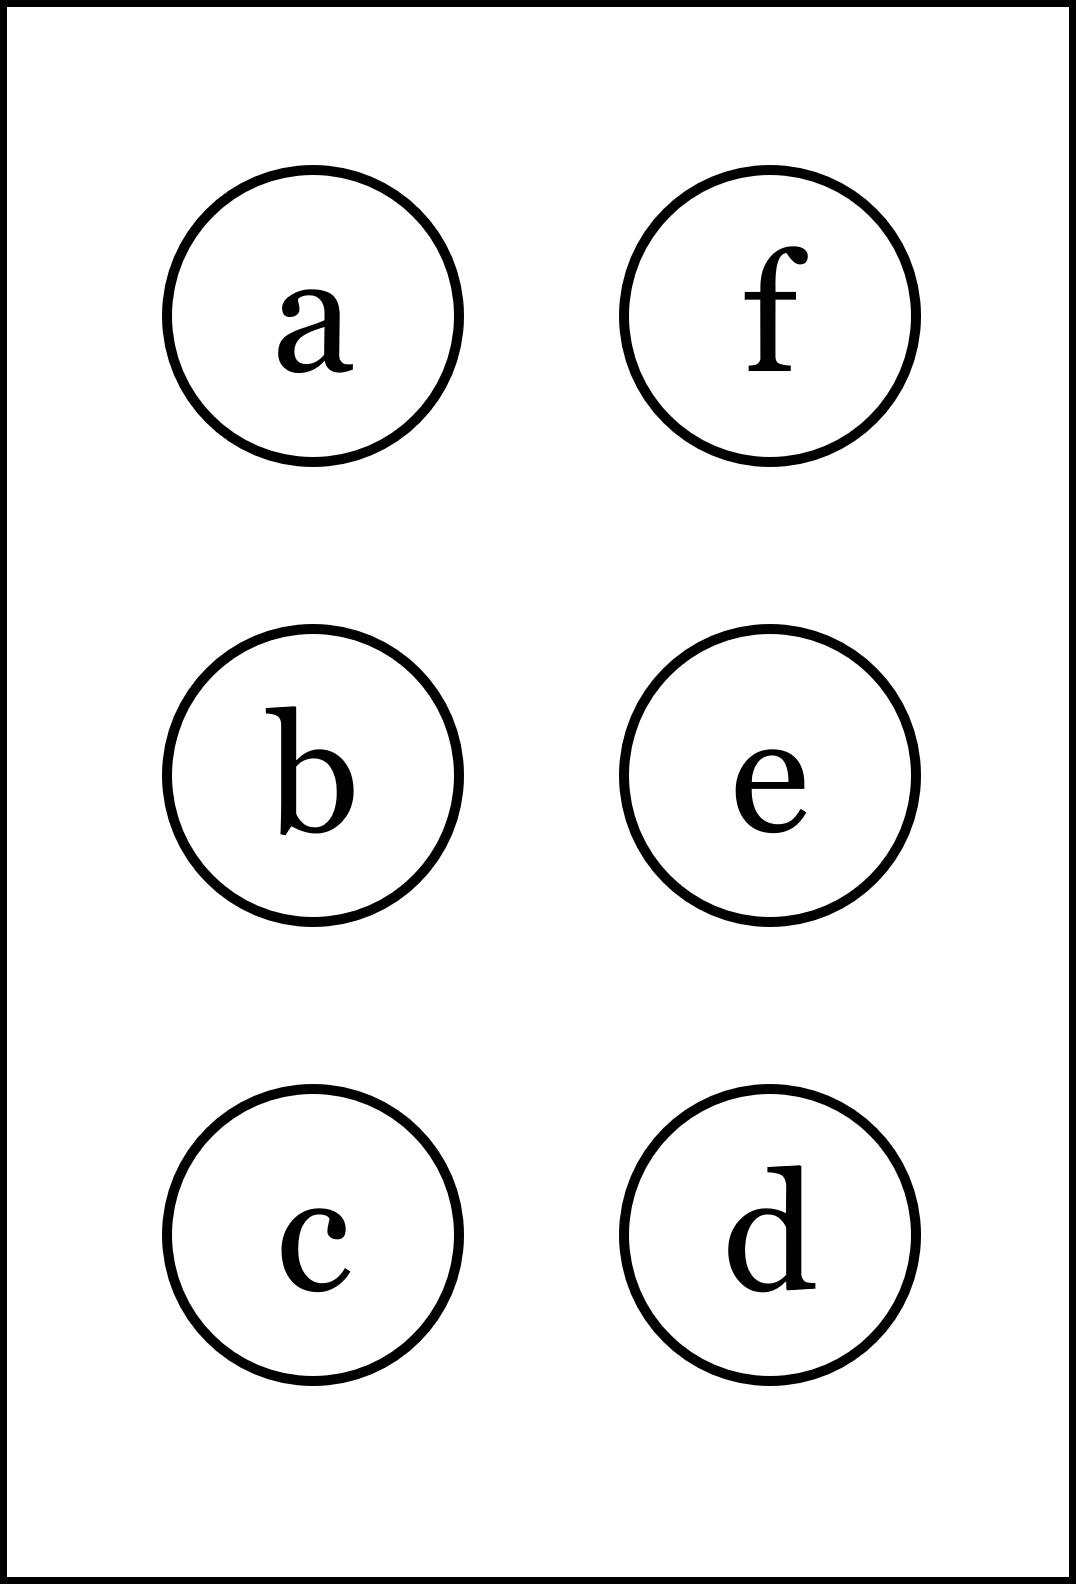
\includegraphics[height=40mm]{../images/braille.png}
{\small Písmeno Braillovej abecedy}
\end{center}
\end{minipage}
\end{center}
\end{minipage}
&
\begin{minipage}[c][104.5mm][t]{0.5\linewidth}
\begin{center}
\vspace{7mm}
{\huge Odmocniny a limity, skupina \textit{Alpha $\alpha$} -\romannumeral2}\\[5mm]
\textit{Jméno:}\phantom{xxxxxxxxxxxxxxxxxxxxxxxxxxxxxxxxxxxxxxxxxxxxxxxxxxxxxxxxxxxxxxxxx}\\[5mm]
\begin{minipage}{0.95\linewidth}
\begin{center}
V \textbf{(a)} a \textbf{(b)} \textbf{uprav výrazy}, v \textbf{(c)} a \textbf{(d)} \textbf{vypočítaj limity}.\\Pokud se výsledky shodujú s tými za otazníky, tak napravo obarvi\\příslušející kroužek načerno. \textbf{Spolu odevzdejte výsledné slovo}.
\end{center}
\end{minipage}
\\[1mm]
\begin{minipage}{0.79\linewidth}
\begin{center}
\begin{varwidth}{\linewidth}
\begin{enumerate}
\small
\item $\sqrt[1]{\left(\cfrac{x^{2}\;x^{\nicefrac{2}{3}}}{x^{-2}}\right)^{6}}$\quad \dotfill\; ???\;\dotfill \quad $x^{28}$
\item {\footnotesize{\scriptsize$\big(\sqrt{6x+6y}+\sqrt{6x-6y}\big)^2-\big(\sqrt{6x+6y}-\sqrt{6x-6y}\big)^2$}\quad \dotfill\; ???\;\dotfill \quad $24\sqrt{x^2-y^2}$}
\item $\lim\limits_{n\to\infty}\cfrac{n^{-1/2}}{\sqrt{9n-5}-\sqrt{9n-7}}$\quad \dotfill\; ???\;\dotfill \quad $3$
\item $\lim\limits_{n\to\infty}3n\cfrac{\sqrt{36n^2+2n-3}-\sqrt{36n^2-7}}{\sqrt{16n^2-4n+3}}$\quad \dotfill\; ???\;\dotfill \quad $\nicefrac{1}{4}$
\item \quad \dotfill\; ???\;\dotfill \quad nebarvi
\item \quad \dotfill\; ???\;\dotfill \quad nebarvi
\end{enumerate}
\end{varwidth}
\end{center}
\end{minipage}
\begin{minipage}{0.20\linewidth}
\begin{center}
{\Huge\bfseries 2.} \\[2mm]
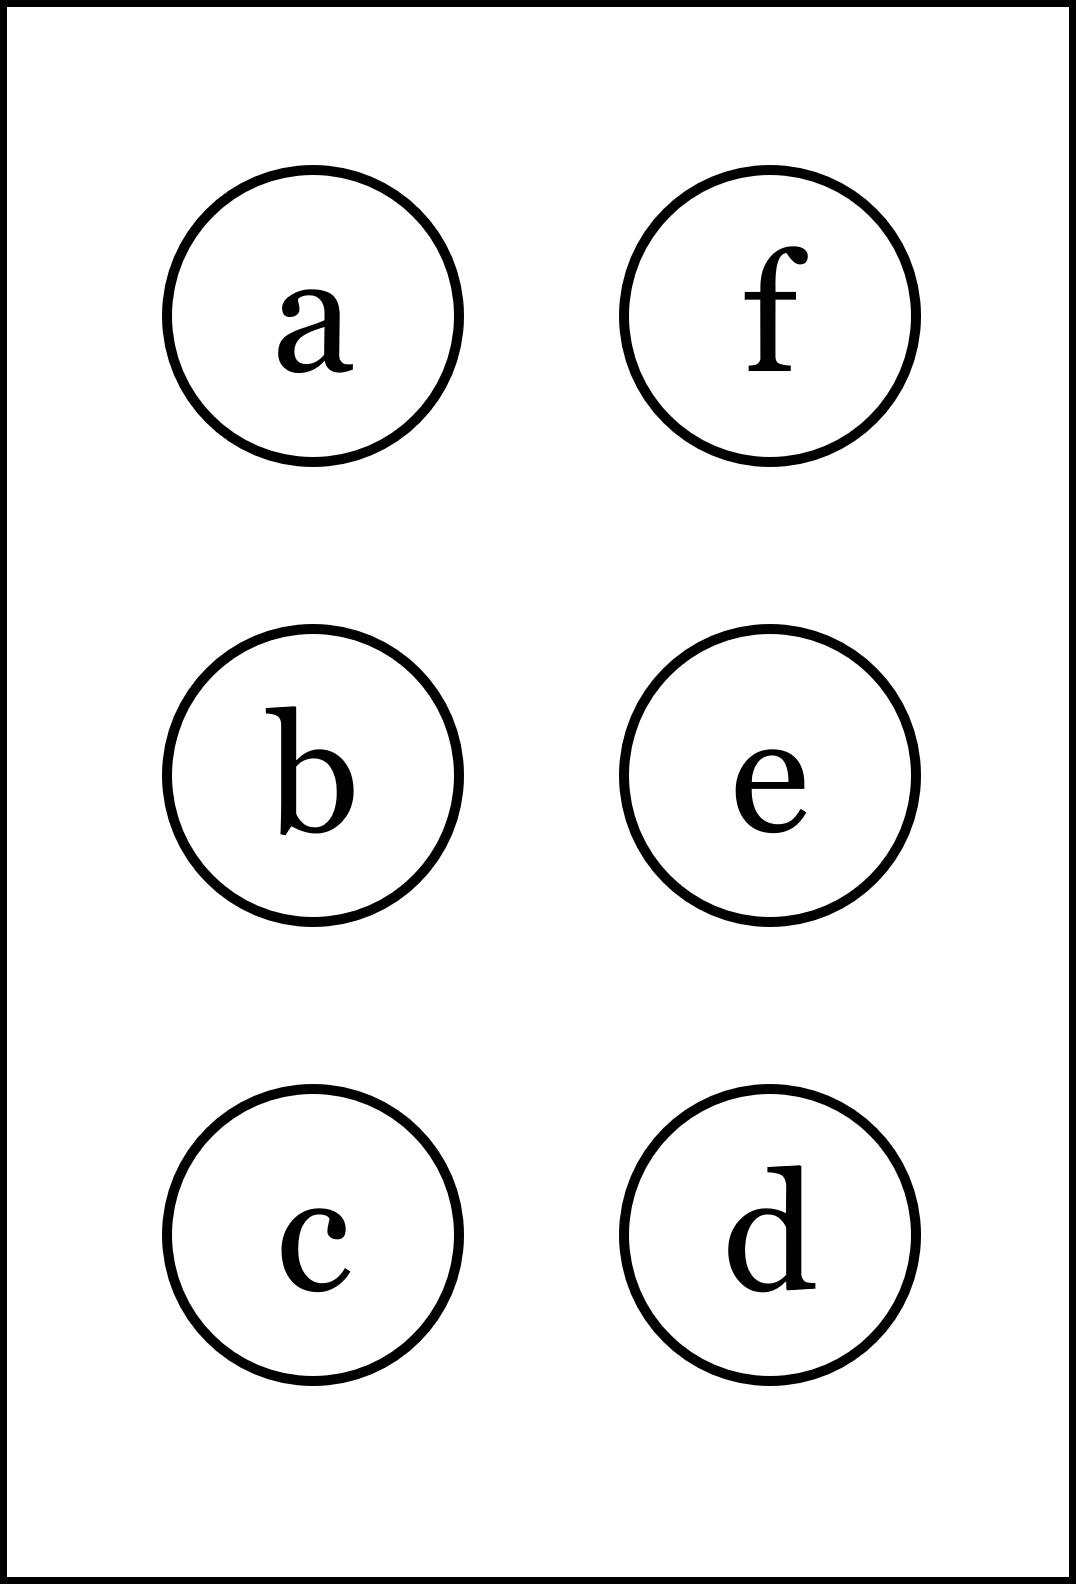
\includegraphics[height=40mm]{../images/braille.png}
{\small Písmeno Braillovej abecedy}
\end{center}
\end{minipage}
\end{center}
\end{minipage}
\\ \hdashline
\begin{minipage}[c][104.5mm][t]{0.5\linewidth}
\begin{center}
\vspace{7mm}
{\huge Odmocniny a limity, skupina \textit{Alpha $\alpha$} -\romannumeral3}\\[5mm]
\textit{Jméno:}\phantom{xxxxxxxxxxxxxxxxxxxxxxxxxxxxxxxxxxxxxxxxxxxxxxxxxxxxxxxxxxxxxxxxx}\\[5mm]
\begin{minipage}{0.95\linewidth}
\begin{center}
V \textbf{(a)} a \textbf{(b)} \textbf{uprav výrazy}, v \textbf{(c)} a \textbf{(d)} \textbf{vypočítaj limity}.\\Pokud se výsledky shodujú s tými za otazníky, tak napravo obarvi\\příslušející kroužek načerno. \textbf{Spolu odevzdejte výsledné slovo}.
\end{center}
\end{minipage}
\\[1mm]
\begin{minipage}{0.79\linewidth}
\begin{center}
\begin{varwidth}{\linewidth}
\begin{enumerate}
\small
\item $\sqrt[1]{\left(\cfrac{x^{-6}\;x^{3}}{x^{-5}}\right)^{2}}$\quad \dotfill\; ???\;\dotfill \quad $x^{4}$
\item {\footnotesize{\scriptsize$\big(\sqrt{x+y}+\sqrt{x-y}\big)^2-\big(\sqrt{x+y}-\sqrt{x-y}\big)^2$}\quad \dotfill\; ???\;\dotfill \quad $2\sqrt{x^2-y^2}$}
\item $\lim\limits_{n\to\infty}\cfrac{n^{-1/2}}{\sqrt{16n-3}-\sqrt{16n+5}}$\quad \dotfill\; ???\;\dotfill \quad $\nicefrac{-1}{2}$
\item $\lim\limits_{n\to\infty}6n\cfrac{\sqrt{4n^2-4n-1}-\sqrt{4n^2-2}}{\sqrt{n^2+3n+2}}$\quad \dotfill\; ???\;\dotfill \quad $-12$
\item \quad \dotfill\; ???\;\dotfill \quad nebarvi
\item \quad \dotfill\; ???\;\dotfill \quad nebarvi
\end{enumerate}
\end{varwidth}
\end{center}
\end{minipage}
\begin{minipage}{0.20\linewidth}
\begin{center}
{\Huge\bfseries 3.} \\[2mm]
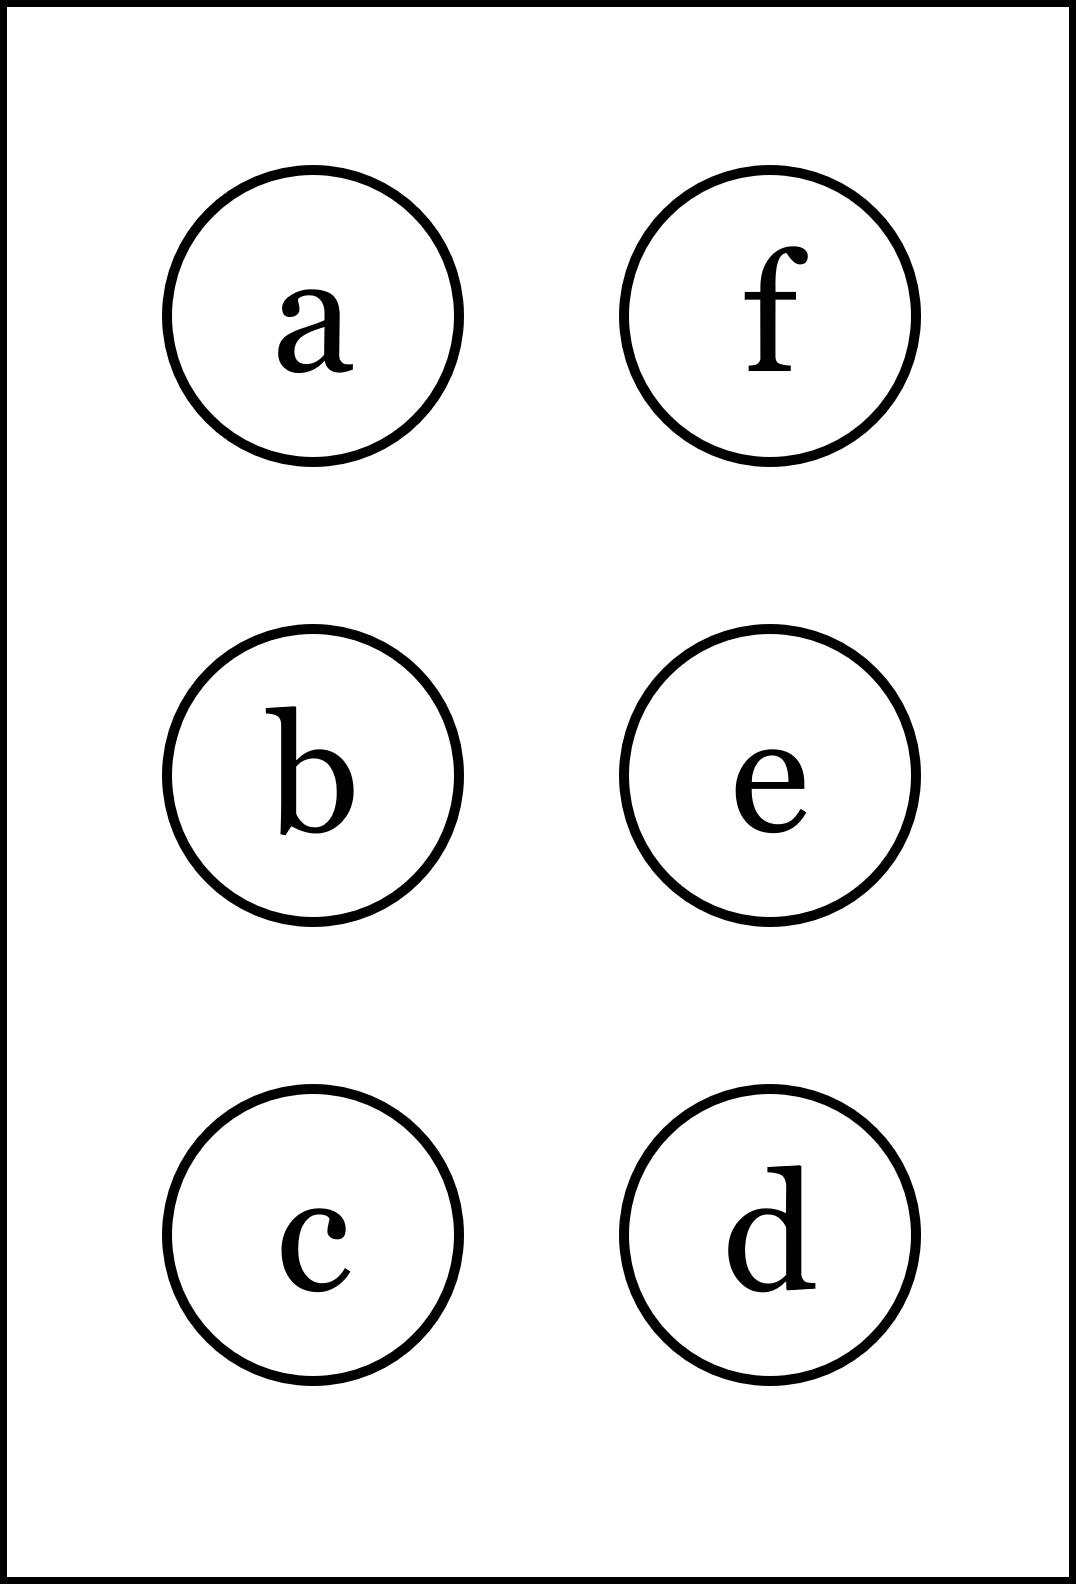
\includegraphics[height=40mm]{../images/braille.png}
{\small Písmeno Braillovej abecedy}
\end{center}
\end{minipage}
\end{center}
\end{minipage}
&
\begin{minipage}[c][104.5mm][t]{0.5\linewidth}
\begin{center}
\vspace{7mm}
{\huge Odmocniny a limity, skupina \textit{Alpha $\alpha$} -\romannumeral4}\\[5mm]
\textit{Jméno:}\phantom{xxxxxxxxxxxxxxxxxxxxxxxxxxxxxxxxxxxxxxxxxxxxxxxxxxxxxxxxxxxxxxxxx}\\[5mm]
\begin{minipage}{0.95\linewidth}
\begin{center}
V \textbf{(a)} a \textbf{(b)} \textbf{uprav výrazy}, v \textbf{(c)} a \textbf{(d)} \textbf{vypočítaj limity}.\\Pokud se výsledky shodujú s tými za otazníky, tak napravo obarvi\\příslušející kroužek načerno. \textbf{Spolu odevzdejte výsledné slovo}.
\end{center}
\end{minipage}
\\[1mm]
\begin{minipage}{0.79\linewidth}
\begin{center}
\begin{varwidth}{\linewidth}
\begin{enumerate}
\small
\item $\sqrt[6]{\left(\cfrac{x^{2}\;x^{\nicefrac{-3}{5}}}{x^{-1}}\right)^{3}}$\quad \dotfill\; ???\;\dotfill \quad $x^{\nicefrac{6}{5}}$
\item {\footnotesize{\scriptsize$\big(\sqrt{3x-9y}+\sqrt{3x+9y}\big)^2-\big(\sqrt{3x-9y}-\sqrt{3x+9y}\big)^2$}\quad \dotfill\; ???\;\dotfill \quad $12\sqrt{x^2+3y^2}$}
\item $\lim\limits_{n\to\infty}\cfrac{n^{-1/2}}{\sqrt{n+6}-\sqrt{n+4}}$\quad \dotfill\; ???\;\dotfill \quad $1$
\item $\lim\limits_{n\to\infty}4n\cfrac{\sqrt{16n^2+5n+2}-\sqrt{16n^2+4}}{\sqrt{n^2-n+1}}$\quad \dotfill\; ???\;\dotfill \quad $5$
\item \quad \dotfill\; ???\;\dotfill \quad nebarvi
\item \quad \dotfill\; ???\;\dotfill \quad nebarvi
\end{enumerate}
\end{varwidth}
\end{center}
\end{minipage}
\begin{minipage}{0.20\linewidth}
\begin{center}
{\Huge\bfseries 4.} \\[2mm]
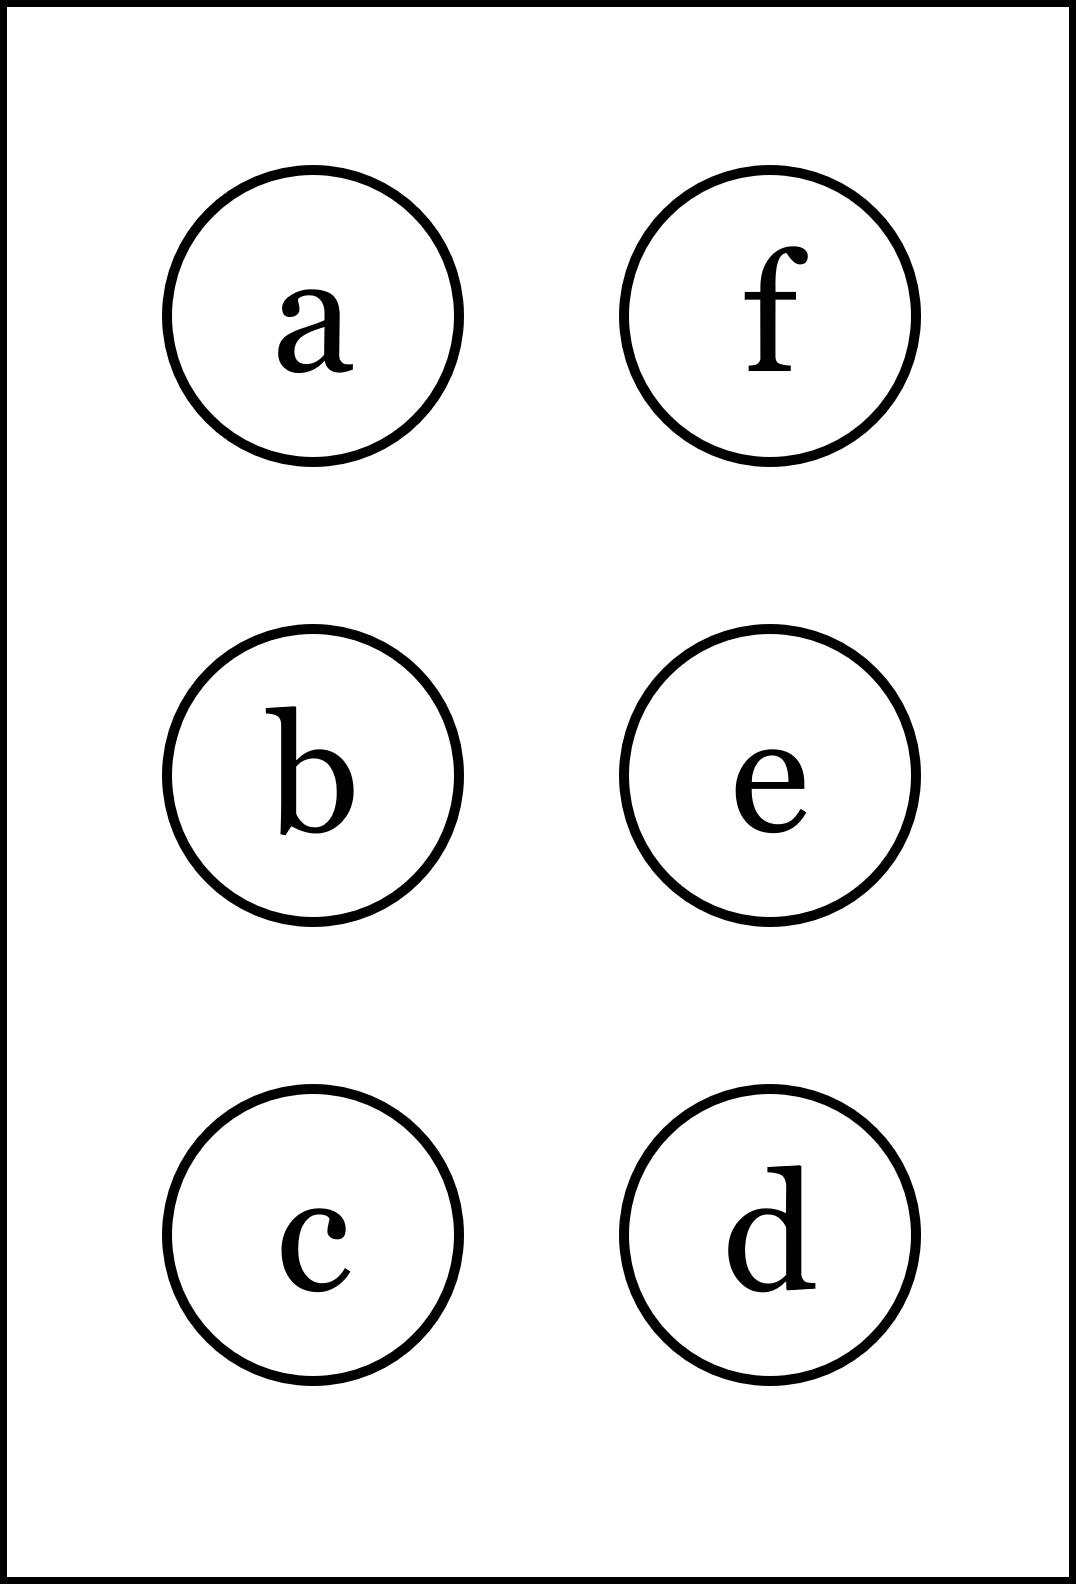
\includegraphics[height=40mm]{../images/braille.png}
{\small Písmeno Braillovej abecedy}
\end{center}
\end{minipage}
\end{center}
\end{minipage}
%
\end{tabular}
\newpage
\thispagestyle{empty}
\begin{tabular}{c:c}
\begin{minipage}[c][104.5mm][t]{0.5\linewidth}
\begin{center}
\vspace{7mm}
{\huge Odmocniny a limity, skupina \textit{Beta $\beta$} -\romannumeral1}\\[5mm]
\textit{Jméno:}\phantom{xxxxxxxxxxxxxxxxxxxxxxxxxxxxxxxxxxxxxxxxxxxxxxxxxxxxxxxxxxxxxxxxx}\\[5mm]
\begin{minipage}{0.95\linewidth}
\begin{center}
V \textbf{(a)} a \textbf{(b)} \textbf{uprav výrazy}, v \textbf{(c)} a \textbf{(d)} \textbf{vypočítaj limity}.\\Pokud se výsledky shodujú s tými za otazníky, tak napravo obarvi\\příslušející kroužek načerno. \textbf{Spolu odevzdejte výsledné slovo}.
\end{center}
\end{minipage}
\\[1mm]
\begin{minipage}{0.79\linewidth}
\begin{center}
\begin{varwidth}{\linewidth}
\begin{enumerate}
\small
\item $\sqrt[3]{\left(\cfrac{x^{1}\;x^{\nicefrac{-2}{5}}}{x^{\nicefrac{-1}{2}}}\right)^{4}}$\quad \dotfill\; ???\;\dotfill \quad $x^{\nicefrac{22}{15}}$
\item {\footnotesize{\scriptsize$\big(\sqrt{8x-8y}+\sqrt{8x+8y}\big)^2-\big(\sqrt{8x-8y}-\sqrt{8x+8y}\big)^2$}\quad \dotfill\; ???\;\dotfill \quad $32\sqrt{x^2+y^2}$}
\item $\lim\limits_{n\to\infty}\cfrac{n^{-1/2}}{\sqrt{36n+7}-\sqrt{36n-2}}$\quad \dotfill\; ???\;\dotfill \quad $\infty$
\item $\lim\limits_{n\to\infty}4n\cfrac{\sqrt{4n^2-5n+1}-\sqrt{4n^2+3}}{\sqrt{9n^2+2n+8}}$\quad \dotfill\; ???\;\dotfill \quad $\nicefrac{-10}{3}$
\item \quad \dotfill\; ???\;\dotfill \quad vybarvi
\item \quad \dotfill\; ???\;\dotfill \quad nebarvi
\end{enumerate}
\end{varwidth}
\end{center}
\end{minipage}
\begin{minipage}{0.20\linewidth}
\begin{center}
{\Huge\bfseries 1.} \\[2mm]
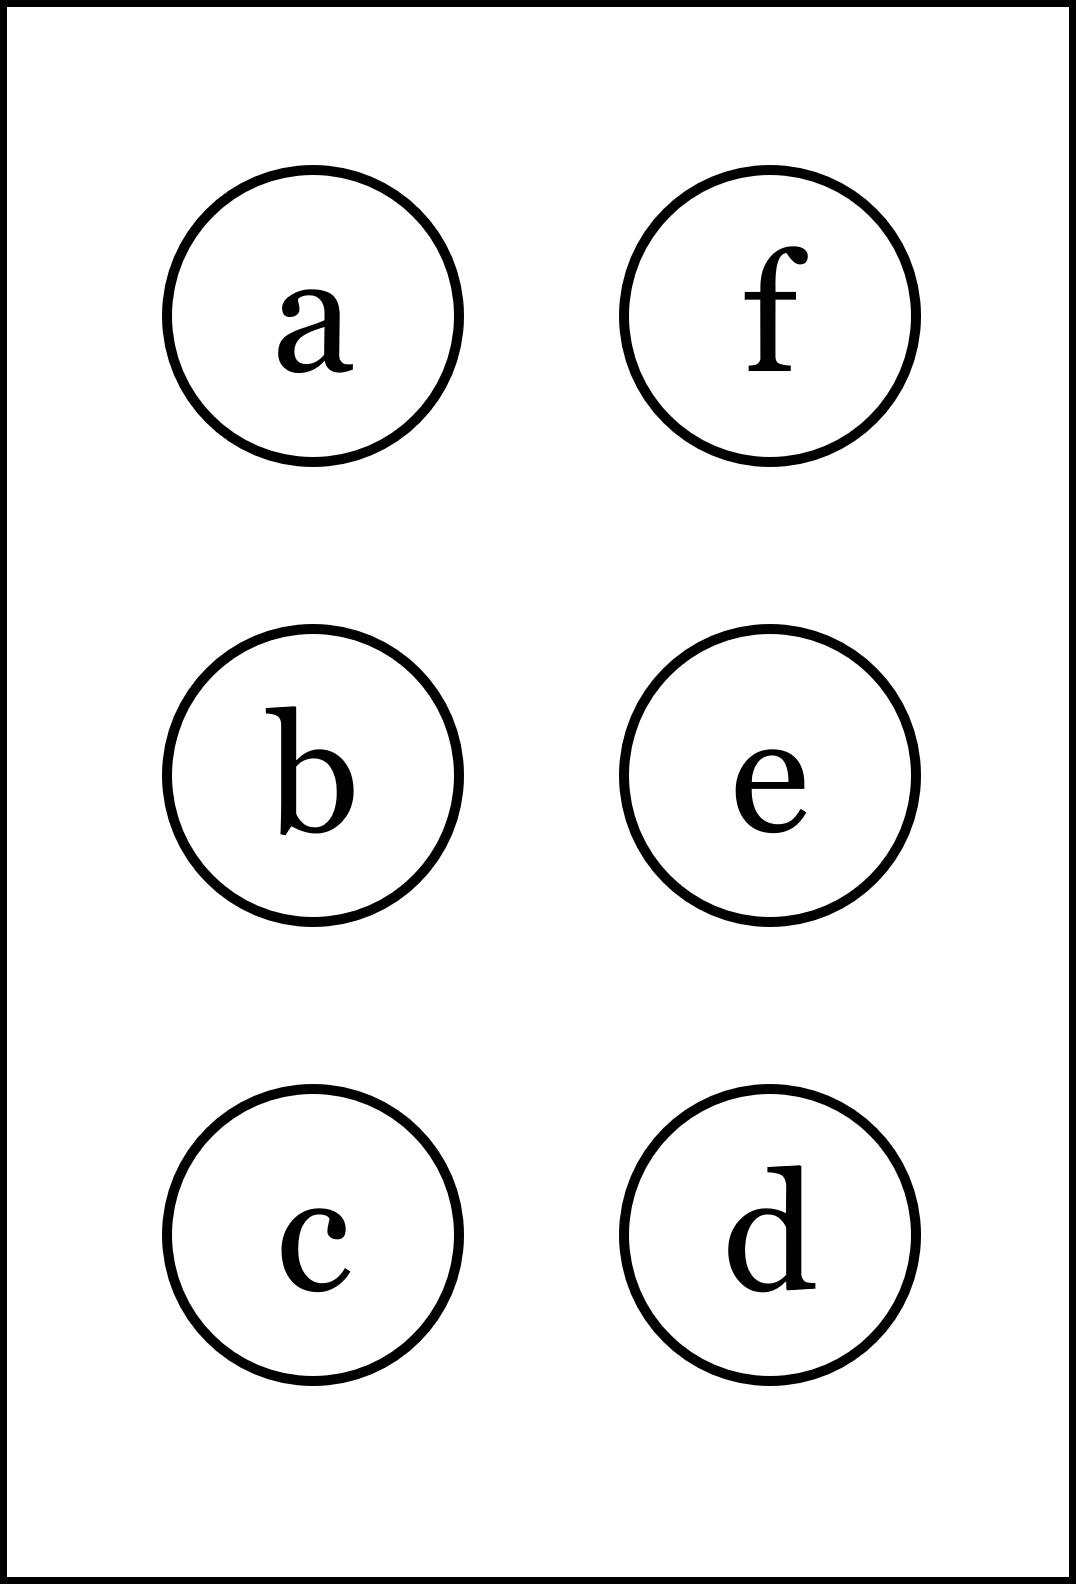
\includegraphics[height=40mm]{../images/braille.png}
{\small Písmeno Braillovej abecedy}
\end{center}
\end{minipage}
\end{center}
\end{minipage}
&
\begin{minipage}[c][104.5mm][t]{0.5\linewidth}
\begin{center}
\vspace{7mm}
{\huge Odmocniny a limity, skupina \textit{Beta $\beta$} -\romannumeral2}\\[5mm]
\textit{Jméno:}\phantom{xxxxxxxxxxxxxxxxxxxxxxxxxxxxxxxxxxxxxxxxxxxxxxxxxxxxxxxxxxxxxxxxx}\\[5mm]
\begin{minipage}{0.95\linewidth}
\begin{center}
V \textbf{(a)} a \textbf{(b)} \textbf{uprav výrazy}, v \textbf{(c)} a \textbf{(d)} \textbf{vypočítaj limity}.\\Pokud se výsledky shodujú s tými za otazníky, tak napravo obarvi\\příslušející kroužek načerno. \textbf{Spolu odevzdejte výsledné slovo}.
\end{center}
\end{minipage}
\\[1mm]
\begin{minipage}{0.79\linewidth}
\begin{center}
\begin{varwidth}{\linewidth}
\begin{enumerate}
\small
\item $\sqrt[6]{\left(\cfrac{x^{-5}\;x^{1}}{x^{4}}\right)^{2}}$\quad \dotfill\; ???\;\dotfill \quad $x^{\nicefrac{-8}{3}}$
\item {\footnotesize{\scriptsize$\big(\sqrt{9x-9y}+\sqrt{9x+9y}\big)^2-\big(\sqrt{9x-9y}-\sqrt{9x+9y}\big)^2$}\quad \dotfill\; ???\;\dotfill \quad $36\sqrt{x^2-y^2}$}
\item $\lim\limits_{n\to\infty}\cfrac{n^{-1/2}}{\sqrt{4n-1}-\sqrt{4n+6}}$\quad \dotfill\; ???\;\dotfill \quad $\nicefrac{-4}{7}$
\item $\lim\limits_{n\to\infty}5n\cfrac{\sqrt{81n^2-7n+1}-\sqrt{81n^2+9}}{\sqrt{64n^2+4n+2}}$\quad \dotfill\; ???\;\dotfill \quad $\nicefrac{-35}{72}$
\item \quad \dotfill\; ???\;\dotfill \quad vybarvi
\item \quad \dotfill\; ???\;\dotfill \quad nebarvi
\end{enumerate}
\end{varwidth}
\end{center}
\end{minipage}
\begin{minipage}{0.20\linewidth}
\begin{center}
{\Huge\bfseries 2.} \\[2mm]
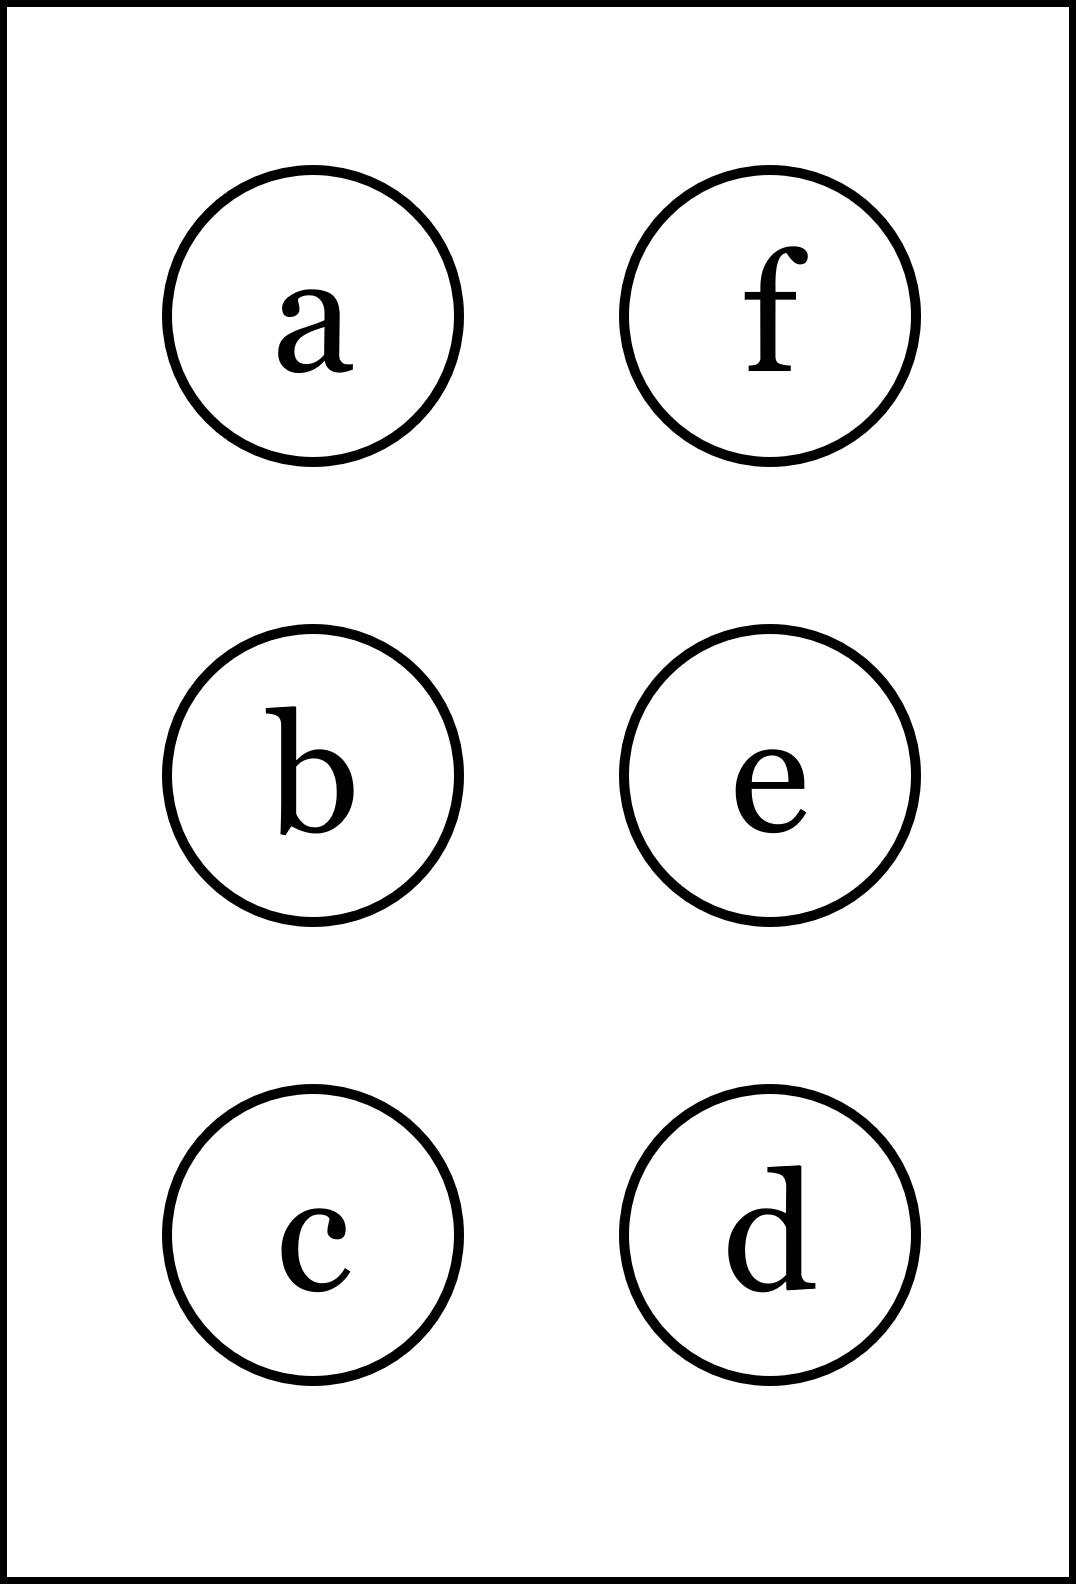
\includegraphics[height=40mm]{../images/braille.png}
{\small Písmeno Braillovej abecedy}
\end{center}
\end{minipage}
\end{center}
\end{minipage}
\\ \hdashline
\begin{minipage}[c][104.5mm][t]{0.5\linewidth}
\begin{center}
\vspace{7mm}
{\huge Odmocniny a limity, skupina \textit{Beta $\beta$} -\romannumeral3}\\[5mm]
\textit{Jméno:}\phantom{xxxxxxxxxxxxxxxxxxxxxxxxxxxxxxxxxxxxxxxxxxxxxxxxxxxxxxxxxxxxxxxxx}\\[5mm]
\begin{minipage}{0.95\linewidth}
\begin{center}
V \textbf{(a)} a \textbf{(b)} \textbf{uprav výrazy}, v \textbf{(c)} a \textbf{(d)} \textbf{vypočítaj limity}.\\Pokud se výsledky shodujú s tými za otazníky, tak napravo obarvi\\příslušející kroužek načerno. \textbf{Spolu odevzdejte výsledné slovo}.
\end{center}
\end{minipage}
\\[1mm]
\begin{minipage}{0.79\linewidth}
\begin{center}
\begin{varwidth}{\linewidth}
\begin{enumerate}
\small
\item $\sqrt[3]{\left(\cfrac{x^{-1}\;x^{\nicefrac{5}{6}}}{x^{-1}}\right)^{2}}$\quad \dotfill\; ???\;\dotfill \quad $x^{\nicefrac{-5}{9}}$
\item {\footnotesize{\scriptsize$\big(\sqrt{x-6y}+\sqrt{x+6y}\big)^2-\big(\sqrt{x-6y}-\sqrt{x+6y}\big)^2$}\quad \dotfill\; ???\;\dotfill \quad $4\sqrt{x^2-36y^2}$}
\item $\lim\limits_{n\to\infty}\cfrac{n^{-1/2}}{\sqrt{9n-3}-\sqrt{9n-4}}$\quad \dotfill\; ???\;\dotfill \quad $\infty$
\item $\lim\limits_{n\to\infty}2n\cfrac{\sqrt{9n^2+3n+8}-\sqrt{9n^2-1}}{\sqrt{64n^2-3n+3}}$\quad \dotfill\; ???\;\dotfill \quad $\nicefrac{1}{4}$
\item \quad \dotfill\; ???\;\dotfill \quad nebarvi
\item \quad \dotfill\; ???\;\dotfill \quad vybarvi
\end{enumerate}
\end{varwidth}
\end{center}
\end{minipage}
\begin{minipage}{0.20\linewidth}
\begin{center}
{\Huge\bfseries 3.} \\[2mm]
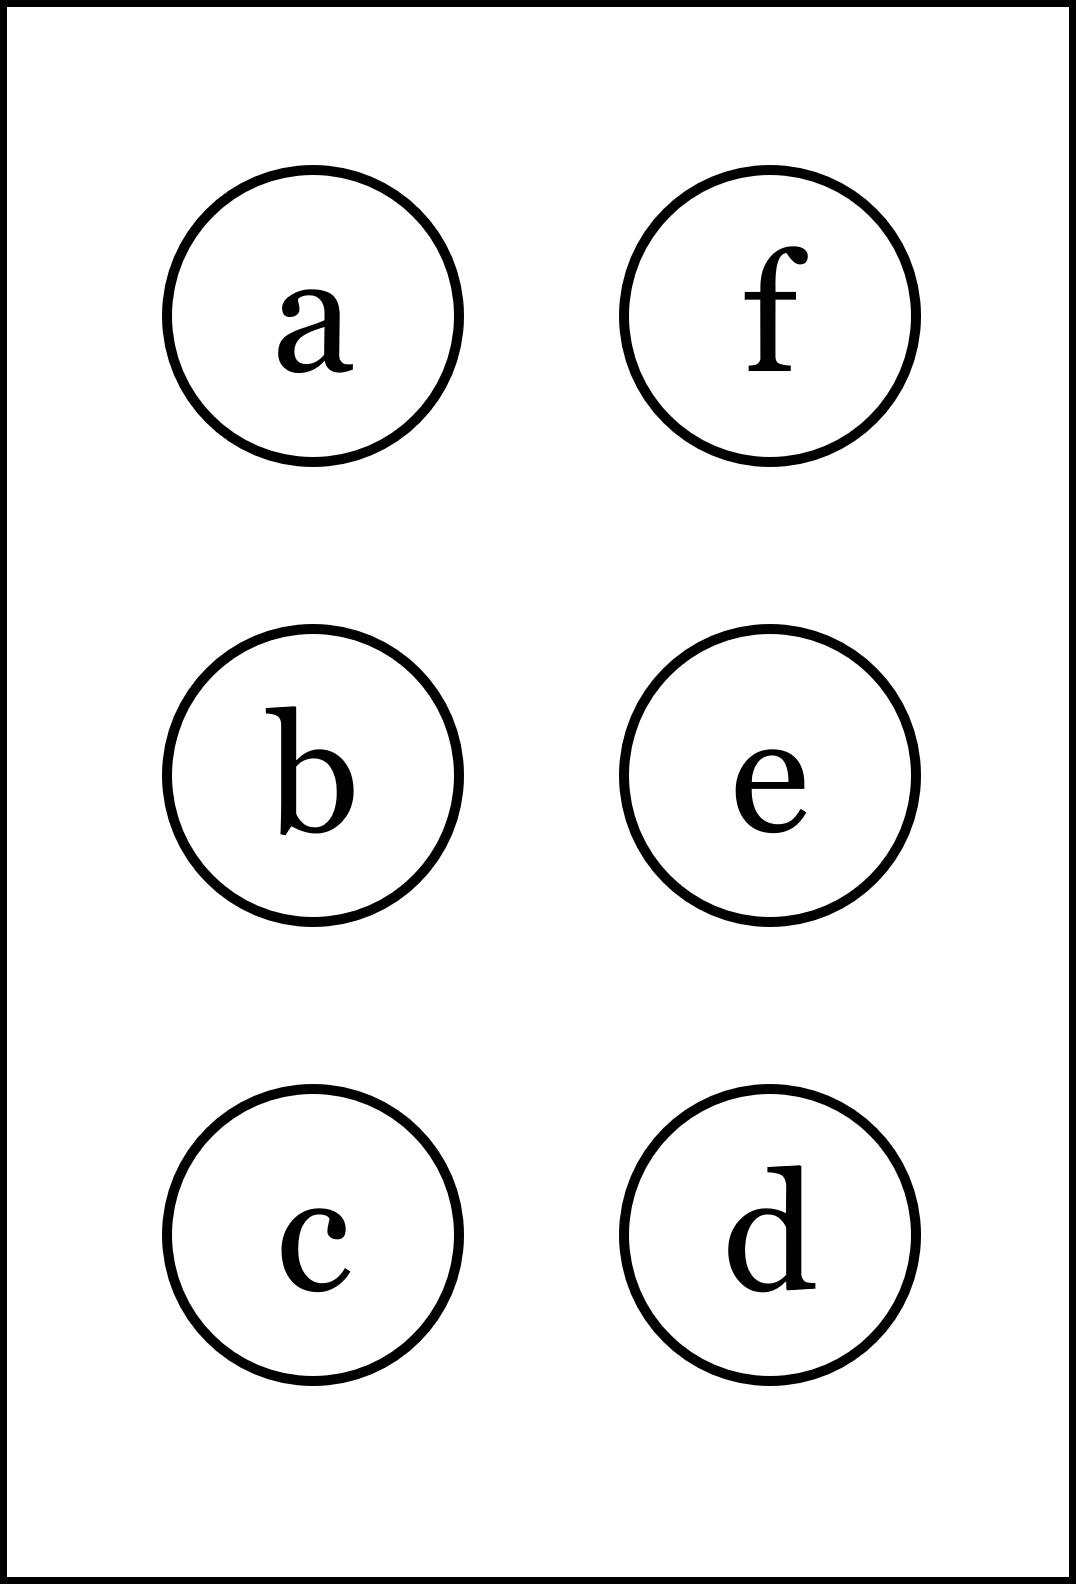
\includegraphics[height=40mm]{../images/braille.png}
{\small Písmeno Braillovej abecedy}
\end{center}
\end{minipage}
\end{center}
\end{minipage}
&
\begin{minipage}[c][104.5mm][t]{0.5\linewidth}
\begin{center}
\vspace{7mm}
{\huge Odmocniny a limity, skupina \textit{Beta $\beta$} -\romannumeral4}\\[5mm]
\textit{Jméno:}\phantom{xxxxxxxxxxxxxxxxxxxxxxxxxxxxxxxxxxxxxxxxxxxxxxxxxxxxxxxxxxxxxxxxx}\\[5mm]
\begin{minipage}{0.95\linewidth}
\begin{center}
V \textbf{(a)} a \textbf{(b)} \textbf{uprav výrazy}, v \textbf{(c)} a \textbf{(d)} \textbf{vypočítaj limity}.\\Pokud se výsledky shodujú s tými za otazníky, tak napravo obarvi\\příslušející kroužek načerno. \textbf{Spolu odevzdejte výsledné slovo}.
\end{center}
\end{minipage}
\\[1mm]
\begin{minipage}{0.79\linewidth}
\begin{center}
\begin{varwidth}{\linewidth}
\begin{enumerate}
\small
\item $\sqrt[1]{\left(\cfrac{x^{\nicefrac{-3}{2}}\;x^{-1}}{x^{\nicefrac{5}{7}}}\right)^{2}}$\quad \dotfill\; ???\;\dotfill \quad $x^{\nicefrac{-45}{7}}$
\item {\footnotesize{\scriptsize$\big(\sqrt{x-2y}+\sqrt{x+2y}\big)^2-\big(\sqrt{x-2y}-\sqrt{x+2y}\big)^2$}\quad \dotfill\; ???\;\dotfill \quad $4\sqrt{x^2+2y^2}$}
\item $\lim\limits_{n\to\infty}\cfrac{n^{-1/2}}{\sqrt{16n-2}-\sqrt{16n+3}}$\quad \dotfill\; ???\;\dotfill \quad $\nicefrac{-8}{5}$
\item $\lim\limits_{n\to\infty}7n\cfrac{\sqrt{49n^2-8n-2}-\sqrt{49n^2-7}}{\sqrt{n^2-6n+5}}$\quad \dotfill\; ???\;\dotfill \quad $-8$
\item \quad \dotfill\; ???\;\dotfill \quad nebarvi
\item \quad \dotfill\; ???\;\dotfill \quad nebarvi
\end{enumerate}
\end{varwidth}
\end{center}
\end{minipage}
\begin{minipage}{0.20\linewidth}
\begin{center}
{\Huge\bfseries 4.} \\[2mm]
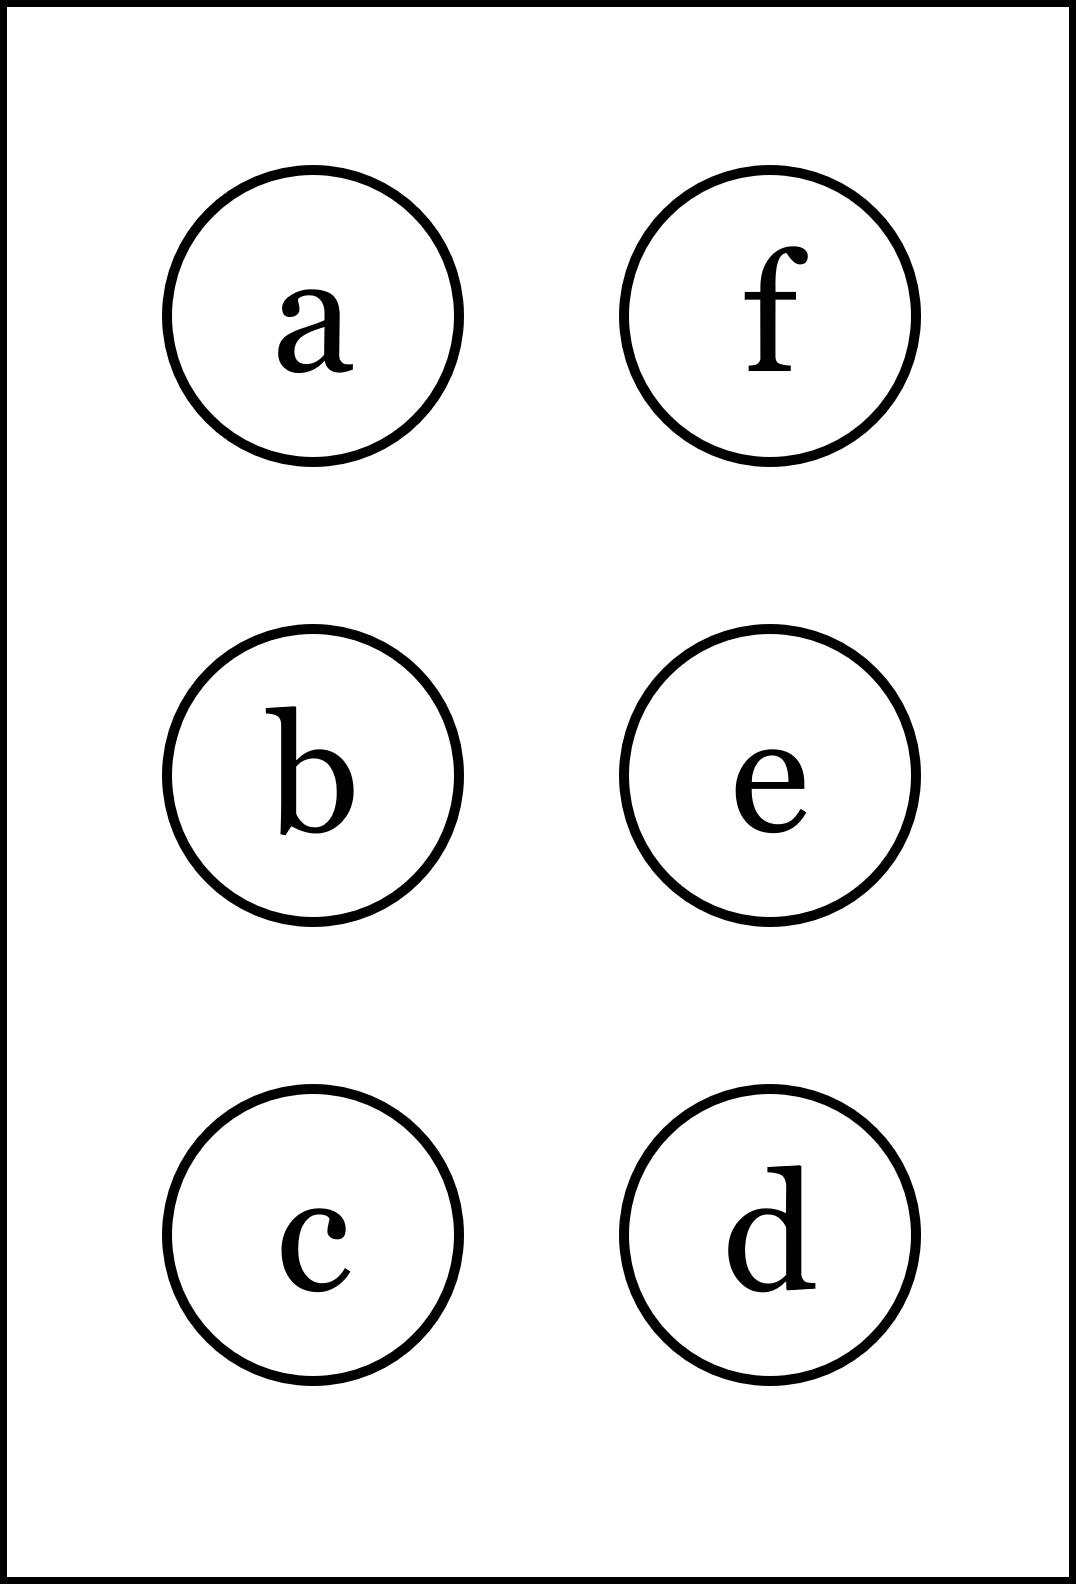
\includegraphics[height=40mm]{../images/braille.png}
{\small Písmeno Braillovej abecedy}
\end{center}
\end{minipage}
\end{center}
\end{minipage}
%
\end{tabular}
\newpage
\thispagestyle{empty}
\begin{tabular}{c:c}
\begin{minipage}[c][104.5mm][t]{0.5\linewidth}
\begin{center}
\vspace{7mm}
{\huge Odmocniny a limity, skupina \textit{Gamma $\gamma$} -\romannumeral1}\\[5mm]
\textit{Jméno:}\phantom{xxxxxxxxxxxxxxxxxxxxxxxxxxxxxxxxxxxxxxxxxxxxxxxxxxxxxxxxxxxxxxxxx}\\[5mm]
\begin{minipage}{0.95\linewidth}
\begin{center}
V \textbf{(a)} a \textbf{(b)} \textbf{uprav výrazy}, v \textbf{(c)} a \textbf{(d)} \textbf{vypočítaj limity}.\\Pokud se výsledky shodujú s tými za otazníky, tak napravo obarvi\\příslušející kroužek načerno. \textbf{Spolu odevzdejte výsledné slovo}.
\end{center}
\end{minipage}
\\[1mm]
\begin{minipage}{0.79\linewidth}
\begin{center}
\begin{varwidth}{\linewidth}
\begin{enumerate}
\small
\item $\sqrt[3]{\left(\cfrac{x^{-1}\;x^{\nicefrac{2}{3}}}{x^{-1}}\right)^{4}}$\quad \dotfill\; ???\;\dotfill \quad $x^{\nicefrac{-8}{9}}$
\item {\footnotesize{\scriptsize$\big(\sqrt{9x-54y}+\sqrt{9x+54y}\big)^2-\big(\sqrt{9x-54y}-\sqrt{9x+54y}\big)^2$}\quad \dotfill\; ???\;\dotfill \quad $36\sqrt{x^2-36y^2}$}
\item $\lim\limits_{n\to\infty}\cfrac{n^{-1/2}}{\sqrt{n+1}-\sqrt{n+4}}$\quad \dotfill\; ???\;\dotfill \quad $\nicefrac{2}{5}$
\item $\lim\limits_{n\to\infty}2n\cfrac{\sqrt{n^2-6n+5}-\sqrt{n^2+2}}{\sqrt{16n^2+3n-7}}$\quad \dotfill\; ???\;\dotfill \quad $-3$
\item \quad \dotfill\; ???\;\dotfill \quad vybarvi
\item \quad \dotfill\; ???\;\dotfill \quad vybarvi
\end{enumerate}
\end{varwidth}
\end{center}
\end{minipage}
\begin{minipage}{0.20\linewidth}
\begin{center}
{\Huge\bfseries 1.} \\[2mm]
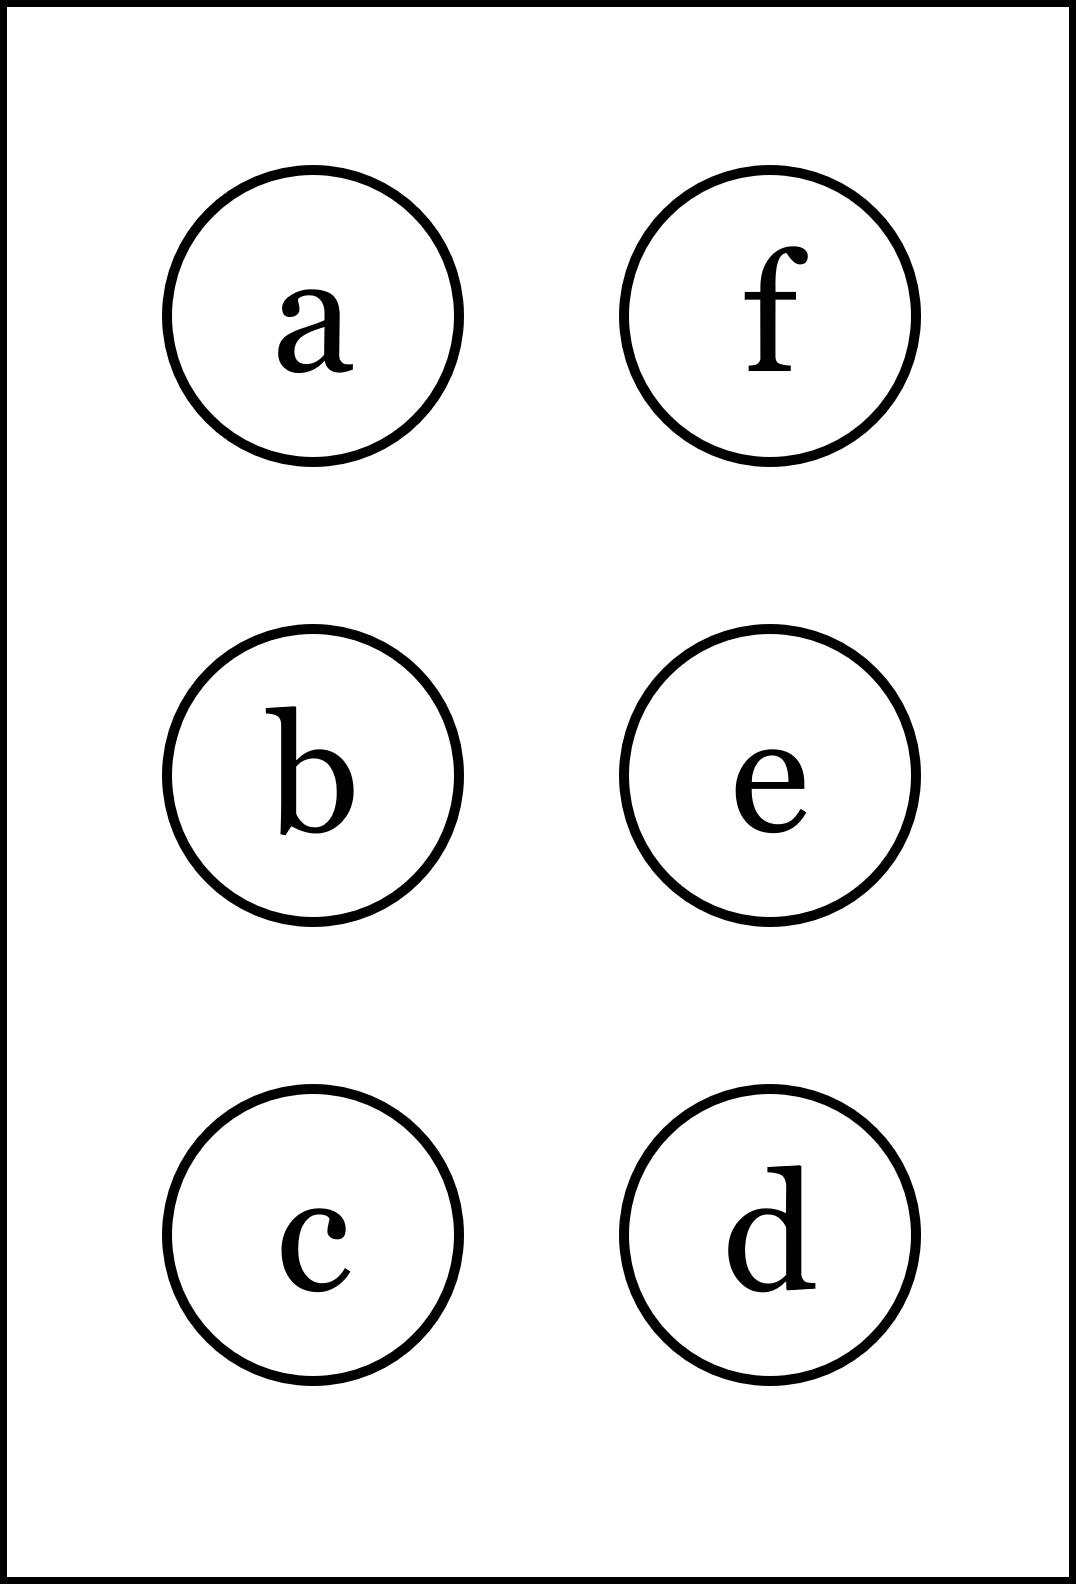
\includegraphics[height=40mm]{../images/braille.png}
{\small Písmeno Braillovej abecedy}
\end{center}
\end{minipage}
\end{center}
\end{minipage}
&
\begin{minipage}[c][104.5mm][t]{0.5\linewidth}
\begin{center}
\vspace{7mm}
{\huge Odmocniny a limity, skupina \textit{Gamma $\gamma$} -\romannumeral2}\\[5mm]
\textit{Jméno:}\phantom{xxxxxxxxxxxxxxxxxxxxxxxxxxxxxxxxxxxxxxxxxxxxxxxxxxxxxxxxxxxxxxxxx}\\[5mm]
\begin{minipage}{0.95\linewidth}
\begin{center}
V \textbf{(a)} a \textbf{(b)} \textbf{uprav výrazy}, v \textbf{(c)} a \textbf{(d)} \textbf{vypočítaj limity}.\\Pokud se výsledky shodujú s tými za otazníky, tak napravo obarvi\\příslušející kroužek načerno. \textbf{Spolu odevzdejte výsledné slovo}.
\end{center}
\end{minipage}
\\[1mm]
\begin{minipage}{0.79\linewidth}
\begin{center}
\begin{varwidth}{\linewidth}
\begin{enumerate}
\small
\item $\sqrt[7]{\left(\cfrac{x^{-4}\;x^{2}}{x^{2}}\right)^{6}}$\quad \dotfill\; ???\;\dotfill \quad $x^{\nicefrac{-24}{7}}$
\item {\footnotesize{\scriptsize$\big(\sqrt{x-2y}+\sqrt{x+2y}\big)^2-\big(\sqrt{x-2y}-\sqrt{x+2y}\big)^2$}\quad \dotfill\; ???\;\dotfill \quad $4\sqrt{x^2+2y^2}$}
\item $\lim\limits_{n\to\infty}\cfrac{n^{-1/2}}{\sqrt{9n+1}-\sqrt{9n-8}}$\quad \dotfill\; ???\;\dotfill \quad $-\infty$
\item $\lim\limits_{n\to\infty}3n\cfrac{\sqrt{9n^2+2n+5}-\sqrt{9n^2-3}}{\sqrt{36n^2-5n-1}}$\quad \dotfill\; ???\;\dotfill \quad $\nicefrac{1}{6}$
\item \quad \dotfill\; ???\;\dotfill \quad nebarvi
\item \quad \dotfill\; ???\;\dotfill \quad nebarvi
\end{enumerate}
\end{varwidth}
\end{center}
\end{minipage}
\begin{minipage}{0.20\linewidth}
\begin{center}
{\Huge\bfseries 2.} \\[2mm]
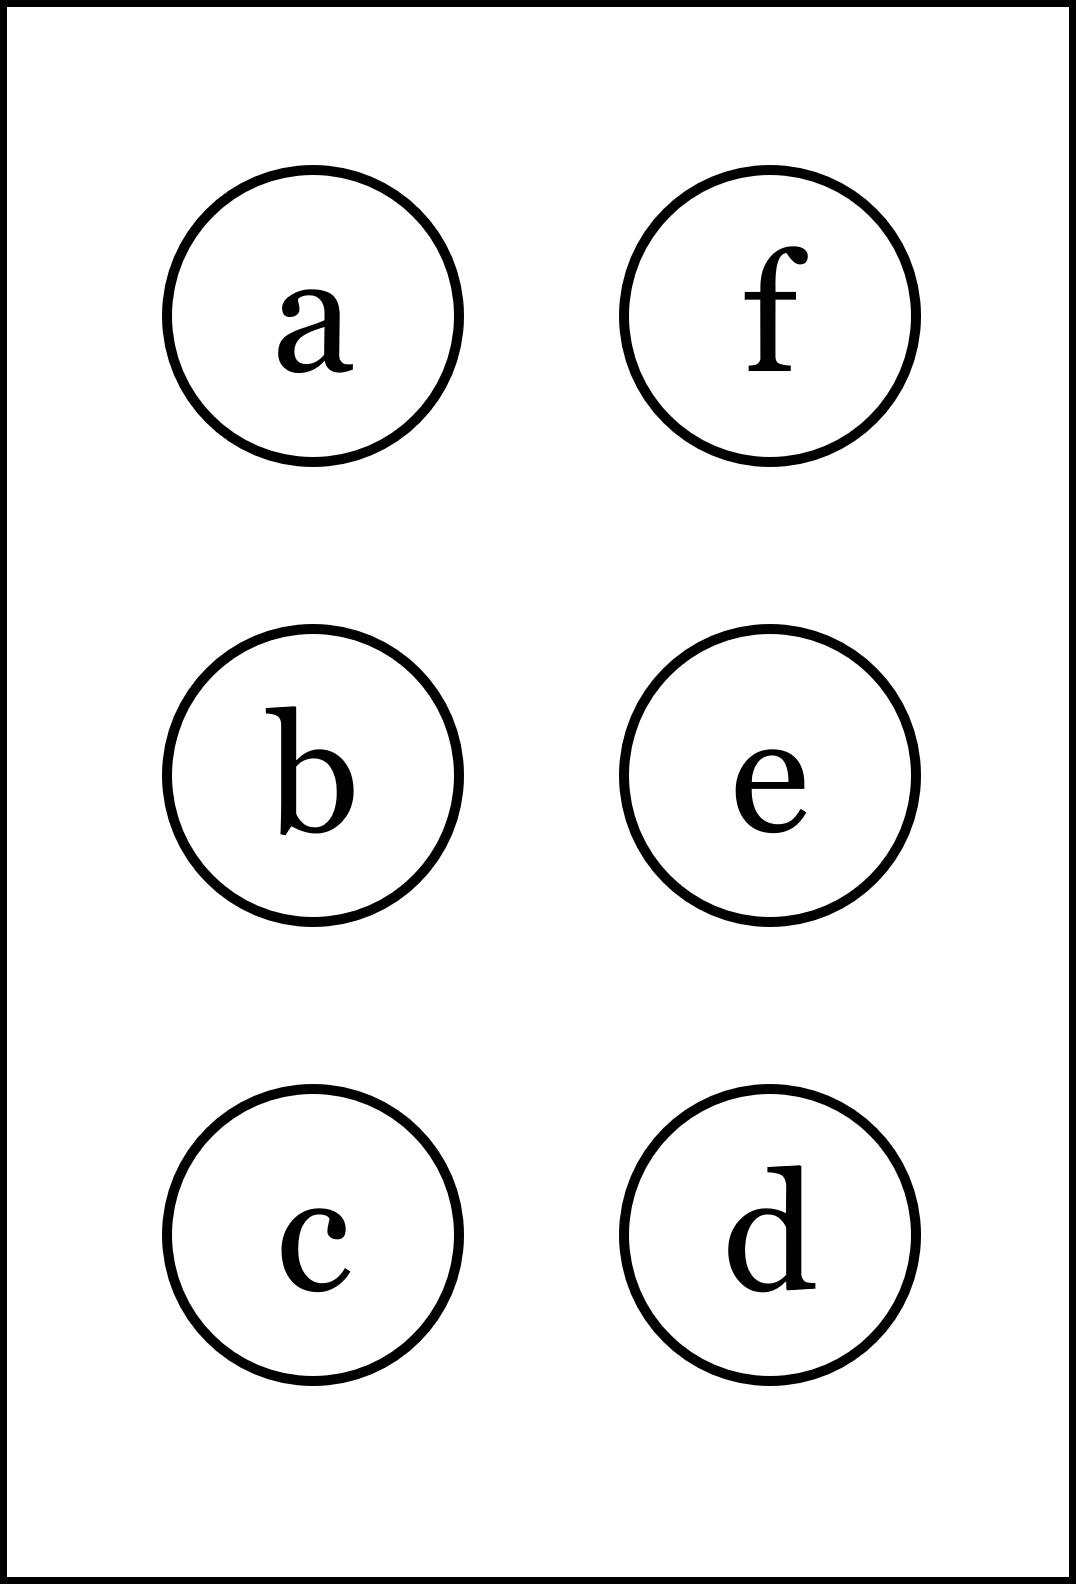
\includegraphics[height=40mm]{../images/braille.png}
{\small Písmeno Braillovej abecedy}
\end{center}
\end{minipage}
\end{center}
\end{minipage}
\\ \hdashline
\begin{minipage}[c][104.5mm][t]{0.5\linewidth}
\begin{center}
\vspace{7mm}
{\huge Odmocniny a limity, skupina \textit{Gamma $\gamma$} -\romannumeral3}\\[5mm]
\textit{Jméno:}\phantom{xxxxxxxxxxxxxxxxxxxxxxxxxxxxxxxxxxxxxxxxxxxxxxxxxxxxxxxxxxxxxxxxx}\\[5mm]
\begin{minipage}{0.95\linewidth}
\begin{center}
V \textbf{(a)} a \textbf{(b)} \textbf{uprav výrazy}, v \textbf{(c)} a \textbf{(d)} \textbf{vypočítaj limity}.\\Pokud se výsledky shodujú s tými za otazníky, tak napravo obarvi\\příslušející kroužek načerno. \textbf{Spolu odevzdejte výsledné slovo}.
\end{center}
\end{minipage}
\\[1mm]
\begin{minipage}{0.79\linewidth}
\begin{center}
\begin{varwidth}{\linewidth}
\begin{enumerate}
\small
\item $\sqrt[3]{\left(\cfrac{x^{-1}\;x^{-2}}{x^{\nicefrac{1}{2}}}\right)^{3}}$\quad \dotfill\; ???\;\dotfill \quad $x^{\nicefrac{-7}{2}}$
\item {\footnotesize{\scriptsize$\big(\sqrt{5x-20y}+\sqrt{5x+20y}\big)^2-\big(\sqrt{5x-20y}-\sqrt{5x+20y}\big)^2$}\quad \dotfill\; ???\;\dotfill \quad $20\sqrt{x^2+4y^2}$}
\item $\lim\limits_{n\to\infty}\cfrac{n^{-1/2}}{\sqrt{n+2}-\sqrt{n+8}}$\quad \dotfill\; ???\;\dotfill \quad $\nicefrac{-1}{3}$
\item $\lim\limits_{n\to\infty}3n\cfrac{\sqrt{16n^2-2n-6}-\sqrt{16n^2-7}}{\sqrt{n^2+2n-3}}$\quad \dotfill\; ???\;\dotfill \quad $\nicefrac{-3}{2}$
\item \quad \dotfill\; ???\;\dotfill \quad nebarvi
\item \quad \dotfill\; ???\;\dotfill \quad vybarvi
\end{enumerate}
\end{varwidth}
\end{center}
\end{minipage}
\begin{minipage}{0.20\linewidth}
\begin{center}
{\Huge\bfseries 3.} \\[2mm]
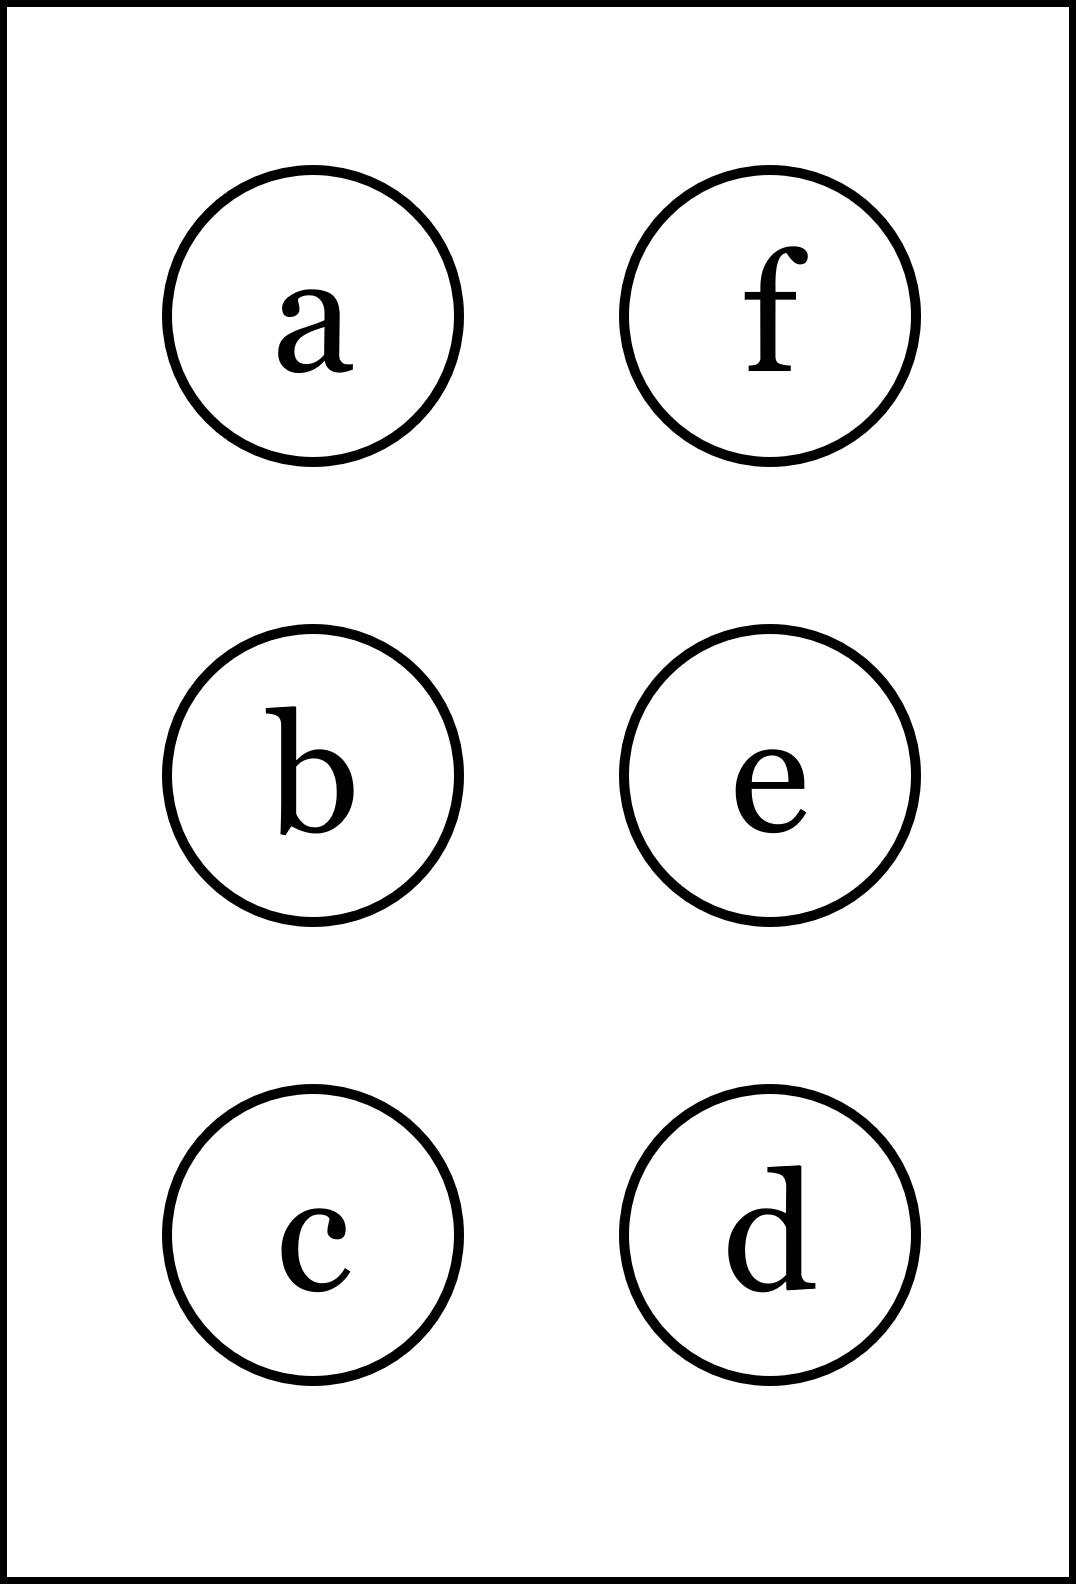
\includegraphics[height=40mm]{../images/braille.png}
{\small Písmeno Braillovej abecedy}
\end{center}
\end{minipage}
\end{center}
\end{minipage}
&
\begin{minipage}[c][104.5mm][t]{0.5\linewidth}
\begin{center}
\vspace{7mm}
{\huge Odmocniny a limity, skupina \textit{Gamma $\gamma$} -\romannumeral4}\\[5mm]
\textit{Jméno:}\phantom{xxxxxxxxxxxxxxxxxxxxxxxxxxxxxxxxxxxxxxxxxxxxxxxxxxxxxxxxxxxxxxxxx}\\[5mm]
\begin{minipage}{0.95\linewidth}
\begin{center}
V \textbf{(a)} a \textbf{(b)} \textbf{uprav výrazy}, v \textbf{(c)} a \textbf{(d)} \textbf{vypočítaj limity}.\\Pokud se výsledky shodujú s tými za otazníky, tak napravo obarvi\\příslušející kroužek načerno. \textbf{Spolu odevzdejte výsledné slovo}.
\end{center}
\end{minipage}
\\[1mm]
\begin{minipage}{0.79\linewidth}
\begin{center}
\begin{varwidth}{\linewidth}
\begin{enumerate}
\small
\item $\sqrt[1]{\left(\cfrac{x^{3}\;x^{\nicefrac{1}{2}}}{x^{6}}\right)^{3}}$\quad \dotfill\; ???\;\dotfill \quad $x^{\nicefrac{-15}{2}}$
\item {\footnotesize{\scriptsize$\big(\sqrt{5x-40y}+\sqrt{5x+40y}\big)^2-\big(\sqrt{5x-40y}-\sqrt{5x+40y}\big)^2$}\quad \dotfill\; ???\;\dotfill \quad $20\sqrt{x^2+8y^2}$}
\item $\lim\limits_{n\to\infty}\cfrac{n^{-1/2}}{\sqrt{n+2}-\sqrt{n-9}}$\quad \dotfill\; ???\;\dotfill \quad $0$
\item $\lim\limits_{n\to\infty}3n\cfrac{\sqrt{64n^2+n+2}-\sqrt{64n^2-9}}{\sqrt{36n^2-3n-2}}$\quad \dotfill\; ???\;\dotfill \quad $\nicefrac{1}{16}$
\item \quad \dotfill\; ???\;\dotfill \quad nebarvi
\item \quad \dotfill\; ???\;\dotfill \quad nebarvi
\end{enumerate}
\end{varwidth}
\end{center}
\end{minipage}
\begin{minipage}{0.20\linewidth}
\begin{center}
{\Huge\bfseries 4.} \\[2mm]
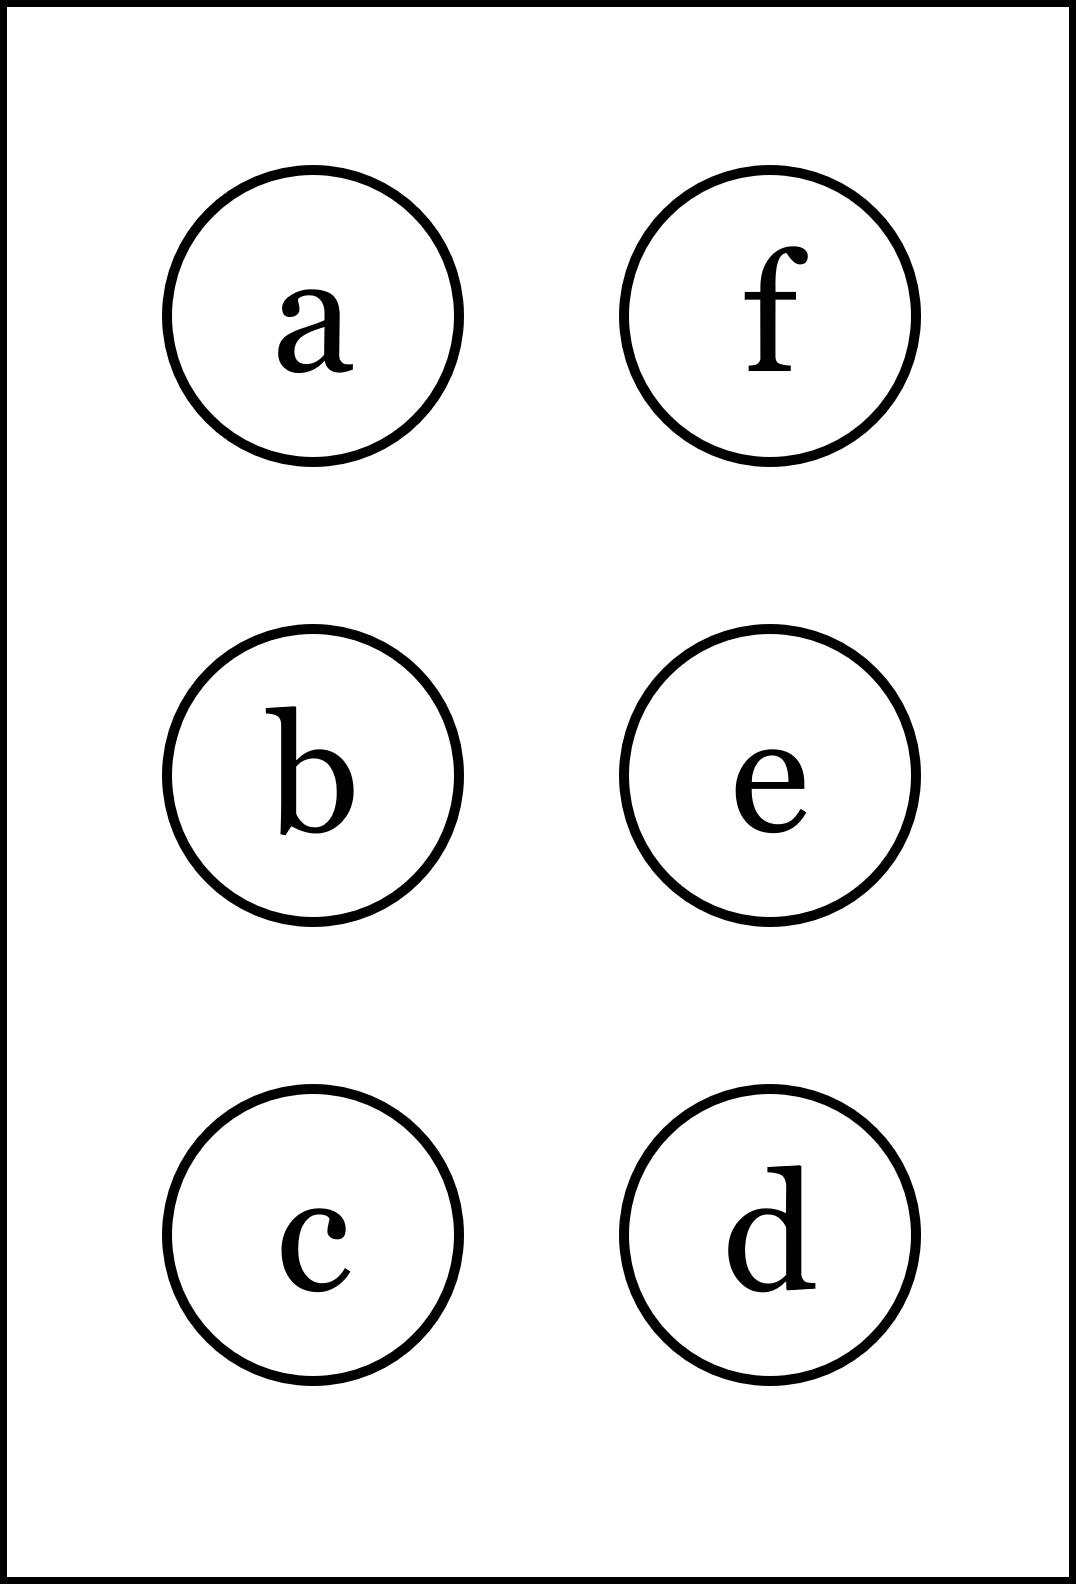
\includegraphics[height=40mm]{../images/braille.png}
{\small Písmeno Braillovej abecedy}
\end{center}
\end{minipage}
\end{center}
\end{minipage}
%
\end{tabular}
\newpage
\thispagestyle{empty}
\begin{tabular}{c:c}
\begin{minipage}[c][104.5mm][t]{0.5\linewidth}
\begin{center}
\vspace{7mm}
{\huge Odmocniny a limity, skupina \textit{Delta $\delta$} -\romannumeral1}\\[5mm]
\textit{Jméno:}\phantom{xxxxxxxxxxxxxxxxxxxxxxxxxxxxxxxxxxxxxxxxxxxxxxxxxxxxxxxxxxxxxxxxx}\\[5mm]
\begin{minipage}{0.95\linewidth}
\begin{center}
V \textbf{(a)} a \textbf{(b)} \textbf{uprav výrazy}, v \textbf{(c)} a \textbf{(d)} \textbf{vypočítaj limity}.\\Pokud se výsledky shodujú s tými za otazníky, tak napravo obarvi\\příslušející kroužek načerno. \textbf{Spolu odevzdejte výsledné slovo}.
\end{center}
\end{minipage}
\\[1mm]
\begin{minipage}{0.79\linewidth}
\begin{center}
\begin{varwidth}{\linewidth}
\begin{enumerate}
\small
\item $\sqrt[5]{\left(\cfrac{x^{\nicefrac{3}{4}}\;x^{\nicefrac{1}{2}}}{x^{2}}\right)^{2}}$\quad \dotfill\; ???\;\dotfill \quad $x^{\nicefrac{-7}{10}}$
\item {\footnotesize{\scriptsize$\big(\sqrt{7x+28y}+\sqrt{7x-28y}\big)^2-\big(\sqrt{7x+28y}-\sqrt{7x-28y}\big)^2$}\quad \dotfill\; ???\;\dotfill \quad $28\sqrt{x^2-16y^2}$}
\item $\lim\limits_{n\to\infty}\cfrac{n^{-1/2}}{\sqrt{25n+9}-\sqrt{25n+3}}$\quad \dotfill\; ???\;\dotfill \quad $\infty$
\item $\lim\limits_{n\to\infty}3n\cfrac{\sqrt{4n^2-n+1}-\sqrt{4n^2-3}}{\sqrt{n^2-n-3}}$\quad \dotfill\; ???\;\dotfill \quad $\nicefrac{-3}{2}$
\item \quad \dotfill\; ???\;\dotfill \quad vybarvi
\item \quad \dotfill\; ???\;\dotfill \quad vybarvi
\end{enumerate}
\end{varwidth}
\end{center}
\end{minipage}
\begin{minipage}{0.20\linewidth}
\begin{center}
{\Huge\bfseries 1.} \\[2mm]
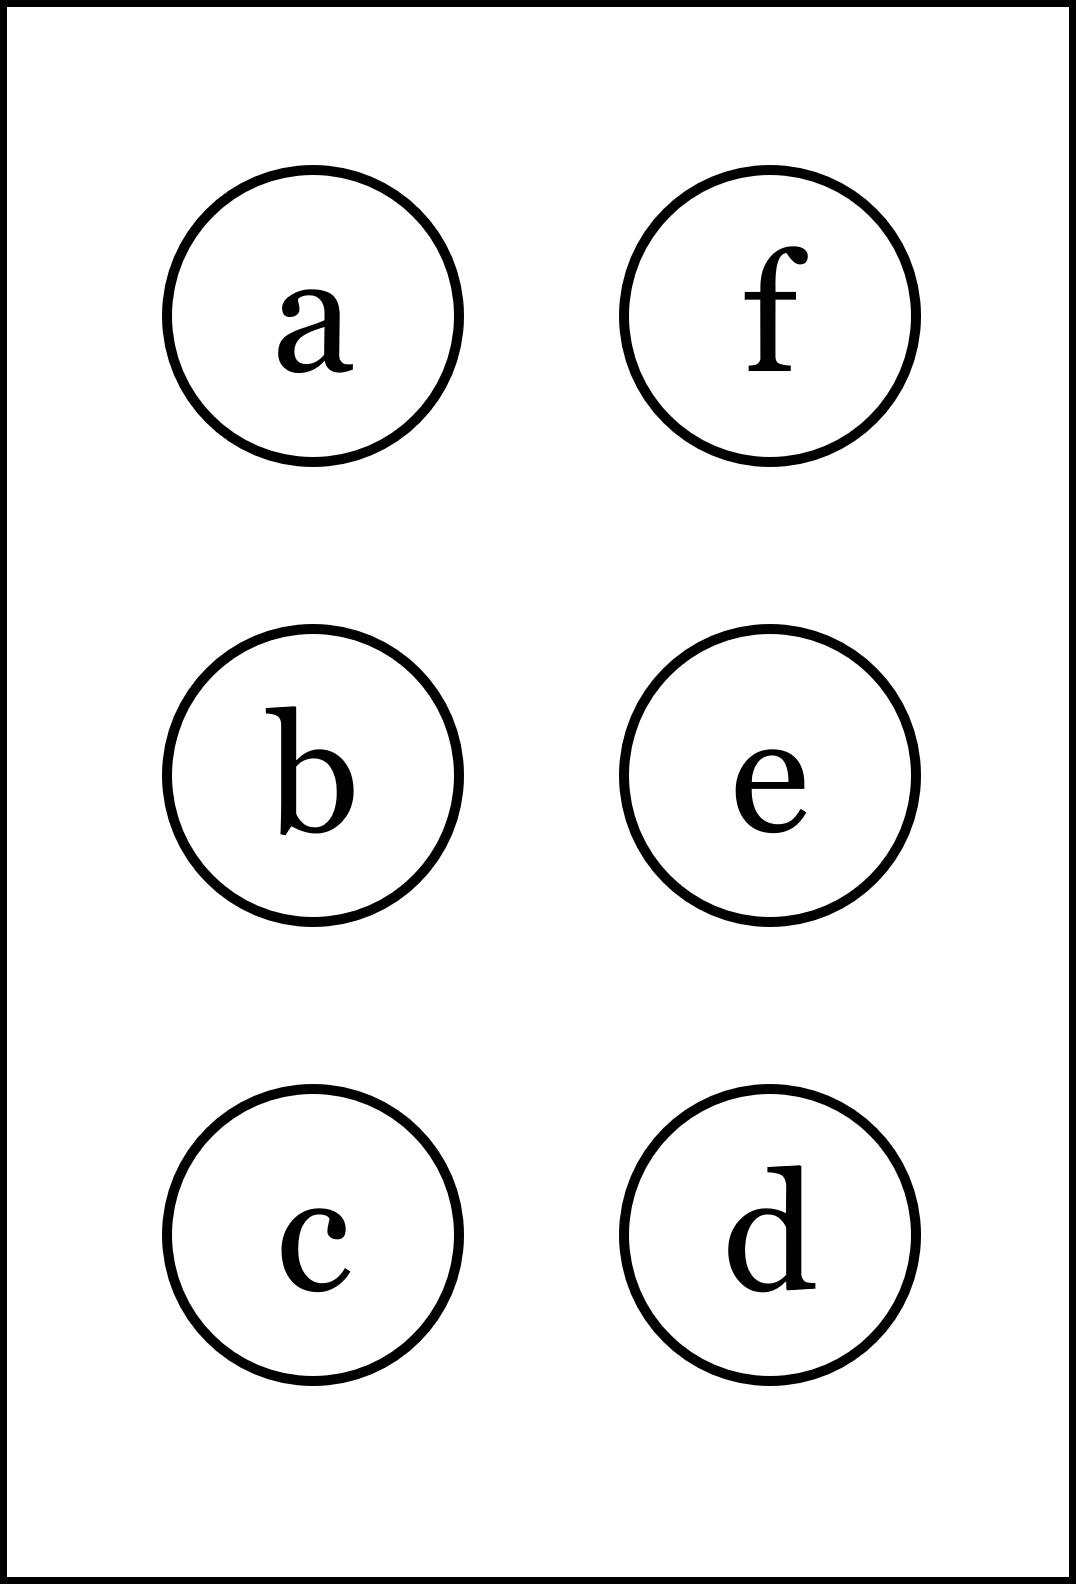
\includegraphics[height=40mm]{../images/braille.png}
{\small Písmeno Braillovej abecedy}
\end{center}
\end{minipage}
\end{center}
\end{minipage}
&
\begin{minipage}[c][104.5mm][t]{0.5\linewidth}
\begin{center}
\vspace{7mm}
{\huge Odmocniny a limity, skupina \textit{Delta $\delta$} -\romannumeral2}\\[5mm]
\textit{Jméno:}\phantom{xxxxxxxxxxxxxxxxxxxxxxxxxxxxxxxxxxxxxxxxxxxxxxxxxxxxxxxxxxxxxxxxx}\\[5mm]
\begin{minipage}{0.95\linewidth}
\begin{center}
V \textbf{(a)} a \textbf{(b)} \textbf{uprav výrazy}, v \textbf{(c)} a \textbf{(d)} \textbf{vypočítaj limity}.\\Pokud se výsledky shodujú s tými za otazníky, tak napravo obarvi\\příslušející kroužek načerno. \textbf{Spolu odevzdejte výsledné slovo}.
\end{center}
\end{minipage}
\\[1mm]
\begin{minipage}{0.79\linewidth}
\begin{center}
\begin{varwidth}{\linewidth}
\begin{enumerate}
\small
\item $\sqrt[5]{\left(\cfrac{x^{-2}\;x^{\nicefrac{3}{4}}}{x^{2}}\right)^{2}}$\quad \dotfill\; ???\;\dotfill \quad $x^{\nicefrac{-13}{10}}$
\item {\footnotesize{\scriptsize$\big(\sqrt{7x-7y}+\sqrt{7x+7y}\big)^2-\big(\sqrt{7x-7y}-\sqrt{7x+7y}\big)^2$}\quad \dotfill\; ???\;\dotfill \quad $28\sqrt{x^2+y^2}$}
\item $\lim\limits_{n\to\infty}\cfrac{n^{-1/2}}{\sqrt{4n+7}-\sqrt{4n-2}}$\quad \dotfill\; ???\;\dotfill \quad $-\infty$
\item $\lim\limits_{n\to\infty}2n\cfrac{\sqrt{81n^2+3n+1}-\sqrt{81n^2-6}}{\sqrt{64n^2+n-1}}$\quad \dotfill\; ???\;\dotfill \quad $\nicefrac{1}{12}$
\item \quad \dotfill\; ???\;\dotfill \quad nebarvi
\item \quad \dotfill\; ???\;\dotfill \quad nebarvi
\end{enumerate}
\end{varwidth}
\end{center}
\end{minipage}
\begin{minipage}{0.20\linewidth}
\begin{center}
{\Huge\bfseries 2.} \\[2mm]
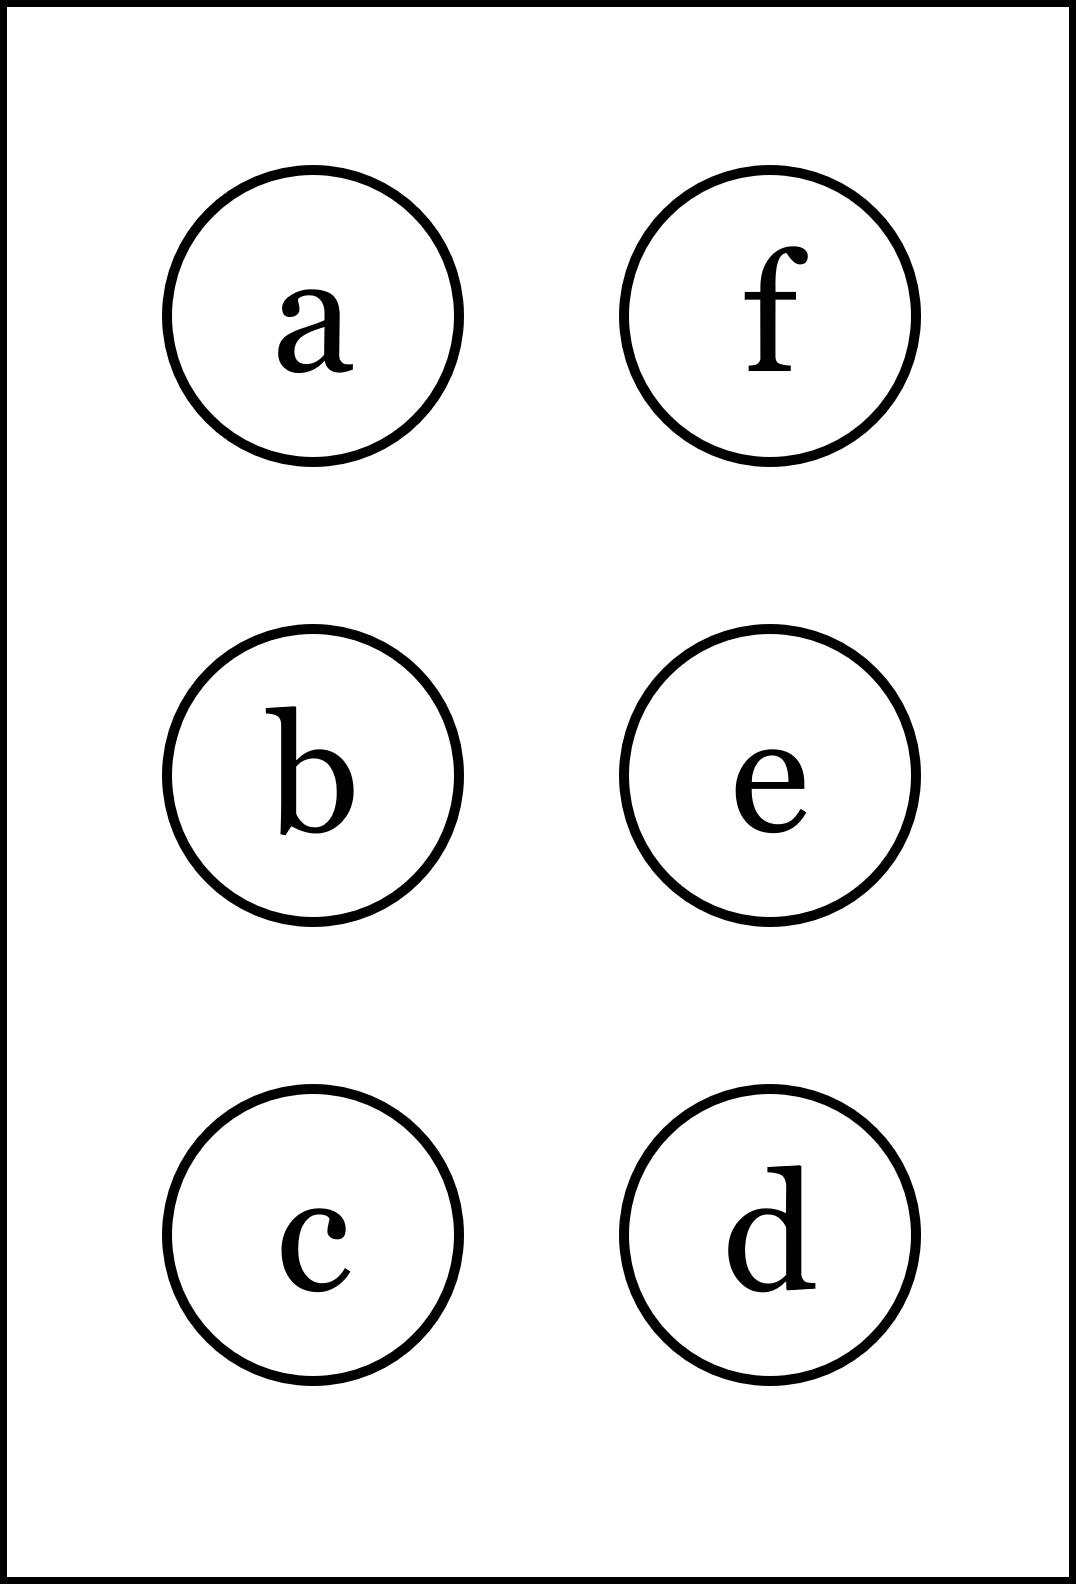
\includegraphics[height=40mm]{../images/braille.png}
{\small Písmeno Braillovej abecedy}
\end{center}
\end{minipage}
\end{center}
\end{minipage}
\\ \hdashline
\begin{minipage}[c][104.5mm][t]{0.5\linewidth}
\begin{center}
\vspace{7mm}
{\huge Odmocniny a limity, skupina \textit{Delta $\delta$} -\romannumeral3}\\[5mm]
\textit{Jméno:}\phantom{xxxxxxxxxxxxxxxxxxxxxxxxxxxxxxxxxxxxxxxxxxxxxxxxxxxxxxxxxxxxxxxxx}\\[5mm]
\begin{minipage}{0.95\linewidth}
\begin{center}
V \textbf{(a)} a \textbf{(b)} \textbf{uprav výrazy}, v \textbf{(c)} a \textbf{(d)} \textbf{vypočítaj limity}.\\Pokud se výsledky shodujú s tými za otazníky, tak napravo obarvi\\příslušející kroužek načerno. \textbf{Spolu odevzdejte výsledné slovo}.
\end{center}
\end{minipage}
\\[1mm]
\begin{minipage}{0.79\linewidth}
\begin{center}
\begin{varwidth}{\linewidth}
\begin{enumerate}
\small
\item $\sqrt[1]{\left(\cfrac{x^{-3}\;x^{2}}{x^{\nicefrac{-3}{4}}}\right)^{3}}$\quad \dotfill\; ???\;\dotfill \quad $x^{\nicefrac{-3}{4}}$
\item {\footnotesize{\scriptsize$\big(\sqrt{4x+32y}+\sqrt{4x-32y}\big)^2-\big(\sqrt{4x+32y}-\sqrt{4x-32y}\big)^2$}\quad \dotfill\; ???\;\dotfill \quad $16\sqrt{x^2-64y^2}$}
\item $\lim\limits_{n\to\infty}\cfrac{n^{-1/2}}{\sqrt{16n-2}-\sqrt{16n+7}}$\quad \dotfill\; ???\;\dotfill \quad $\nicefrac{-8}{9}$
\item $\lim\limits_{n\to\infty}8n\cfrac{\sqrt{4n^2-2n-4}-\sqrt{4n^2-5}}{\sqrt{9n^2-4n-9}}$\quad \dotfill\; ???\;\dotfill \quad $\nicefrac{-8}{3}$
\item \quad \dotfill\; ???\;\dotfill \quad vybarvi
\item \quad \dotfill\; ???\;\dotfill \quad nebarvi
\end{enumerate}
\end{varwidth}
\end{center}
\end{minipage}
\begin{minipage}{0.20\linewidth}
\begin{center}
{\Huge\bfseries 3.} \\[2mm]
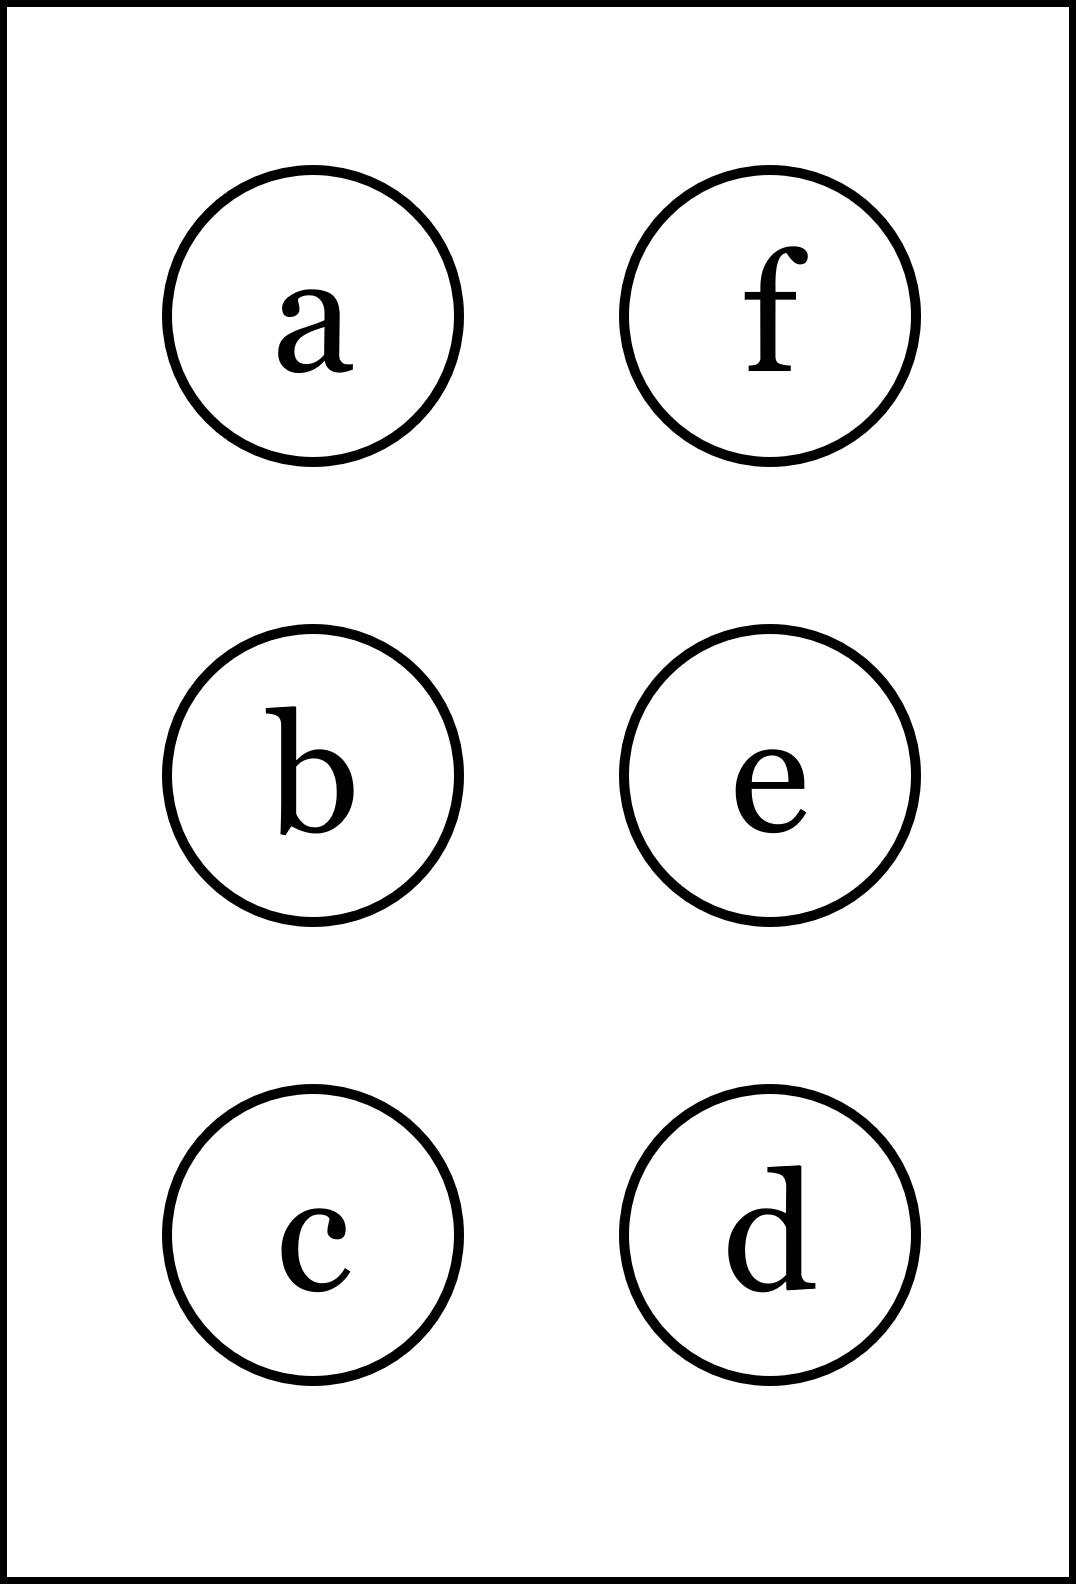
\includegraphics[height=40mm]{../images/braille.png}
{\small Písmeno Braillovej abecedy}
\end{center}
\end{minipage}
\end{center}
\end{minipage}
&
\begin{minipage}[c][104.5mm][t]{0.5\linewidth}
\begin{center}
\vspace{7mm}
{\huge Odmocniny a limity, skupina \textit{Delta $\delta$} -\romannumeral4}\\[5mm]
\textit{Jméno:}\phantom{xxxxxxxxxxxxxxxxxxxxxxxxxxxxxxxxxxxxxxxxxxxxxxxxxxxxxxxxxxxxxxxxx}\\[5mm]
\begin{minipage}{0.95\linewidth}
\begin{center}
V \textbf{(a)} a \textbf{(b)} \textbf{uprav výrazy}, v \textbf{(c)} a \textbf{(d)} \textbf{vypočítaj limity}.\\Pokud se výsledky shodujú s tými za otazníky, tak napravo obarvi\\příslušející kroužek načerno. \textbf{Spolu odevzdejte výsledné slovo}.
\end{center}
\end{minipage}
\\[1mm]
\begin{minipage}{0.79\linewidth}
\begin{center}
\begin{varwidth}{\linewidth}
\begin{enumerate}
\small
\item $\sqrt[4]{\left(\cfrac{x^{1}\;x^{3}}{x^{\nicefrac{-6}{7}}}\right)^{2}}$\quad \dotfill\; ???\;\dotfill \quad $x^{\nicefrac{17}{7}}$
\item {\footnotesize{\scriptsize$\big(\sqrt{4x-8y}+\sqrt{4x+8y}\big)^2-\big(\sqrt{4x-8y}-\sqrt{4x+8y}\big)^2$}\quad \dotfill\; ???\;\dotfill \quad $16\sqrt{x^2+2y^2}$}
\item $\lim\limits_{n\to\infty}\cfrac{n^{-1/2}}{\sqrt{n+6}-\sqrt{n+7}}$\quad \dotfill\; ???\;\dotfill \quad $-2$
\item $\lim\limits_{n\to\infty}6n\cfrac{\sqrt{n^2+2n+8}-\sqrt{n^2-4}}{\sqrt{36n^2+7n+6}}$\quad \dotfill\; ???\;\dotfill \quad $2$
\item \quad \dotfill\; ???\;\dotfill \quad vybarvi
\item \quad \dotfill\; ???\;\dotfill \quad nebarvi
\end{enumerate}
\end{varwidth}
\end{center}
\end{minipage}
\begin{minipage}{0.20\linewidth}
\begin{center}
{\Huge\bfseries 4.} \\[2mm]
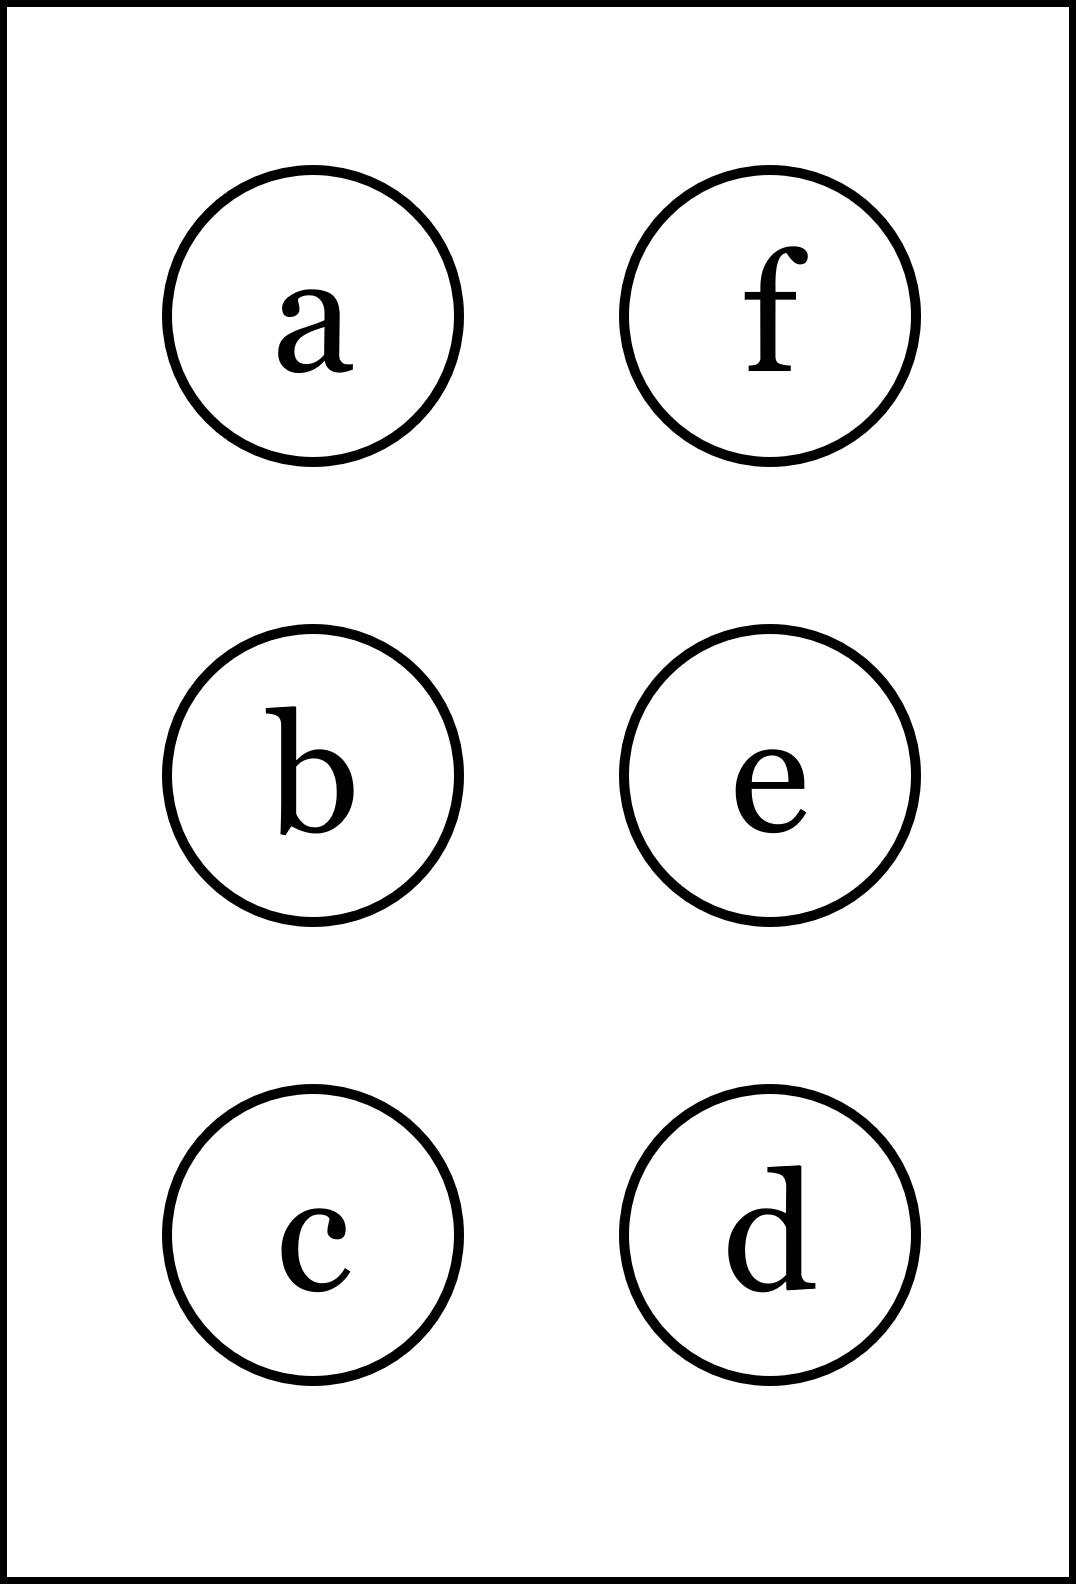
\includegraphics[height=40mm]{../images/braille.png}
{\small Písmeno Braillovej abecedy}
\end{center}
\end{minipage}
\end{center}
\end{minipage}
%
\end{tabular}
\newpage
\thispagestyle{empty}
\begin{tabular}{c:c}
\begin{minipage}[c][104.5mm][t]{0.5\linewidth}
\begin{center}
\vspace{7mm}
{\huge Odmocniny a limity, skupina \textit{Epsilon $\epsilon$} -\romannumeral1}\\[5mm]
\textit{Jméno:}\phantom{xxxxxxxxxxxxxxxxxxxxxxxxxxxxxxxxxxxxxxxxxxxxxxxxxxxxxxxxxxxxxxxxx}\\[5mm]
\begin{minipage}{0.95\linewidth}
\begin{center}
V \textbf{(a)} a \textbf{(b)} \textbf{uprav výrazy}, v \textbf{(c)} a \textbf{(d)} \textbf{vypočítaj limity}.\\Pokud se výsledky shodujú s tými za otazníky, tak napravo obarvi\\příslušející kroužek načerno. \textbf{Spolu odevzdejte výsledné slovo}.
\end{center}
\end{minipage}
\\[1mm]
\begin{minipage}{0.79\linewidth}
\begin{center}
\begin{varwidth}{\linewidth}
\begin{enumerate}
\small
\item $\sqrt[1]{\left(\cfrac{x^{8}\;x^{\nicefrac{1}{2}}}{x^{-2}}\right)^{2}}$\quad \dotfill\; ???\;\dotfill \quad $x^{21}$
\item {\footnotesize{\scriptsize$\big(\sqrt{x-y}+\sqrt{x+y}\big)^2-\big(\sqrt{x-y}-\sqrt{x+y}\big)^2$}\quad \dotfill\; ???\;\dotfill \quad $4\sqrt{x^2-y^2}$}
\item $\lim\limits_{n\to\infty}\cfrac{n^{-1/2}}{\sqrt{9n+6}-\sqrt{9n+4}}$\quad \dotfill\; ???\;\dotfill \quad $3$
\item $\lim\limits_{n\to\infty}2n\cfrac{\sqrt{64n^2+3n-9}-\sqrt{64n^2+4}}{\sqrt{n^2-3n-1}}$\quad \dotfill\; ???\;\dotfill \quad $\nicefrac{3}{8}$
\item \quad \dotfill\; ???\;\dotfill \quad vybarvi
\item \quad \dotfill\; ???\;\dotfill \quad nebarvi
\end{enumerate}
\end{varwidth}
\end{center}
\end{minipage}
\begin{minipage}{0.20\linewidth}
\begin{center}
{\Huge\bfseries 1.} \\[2mm]
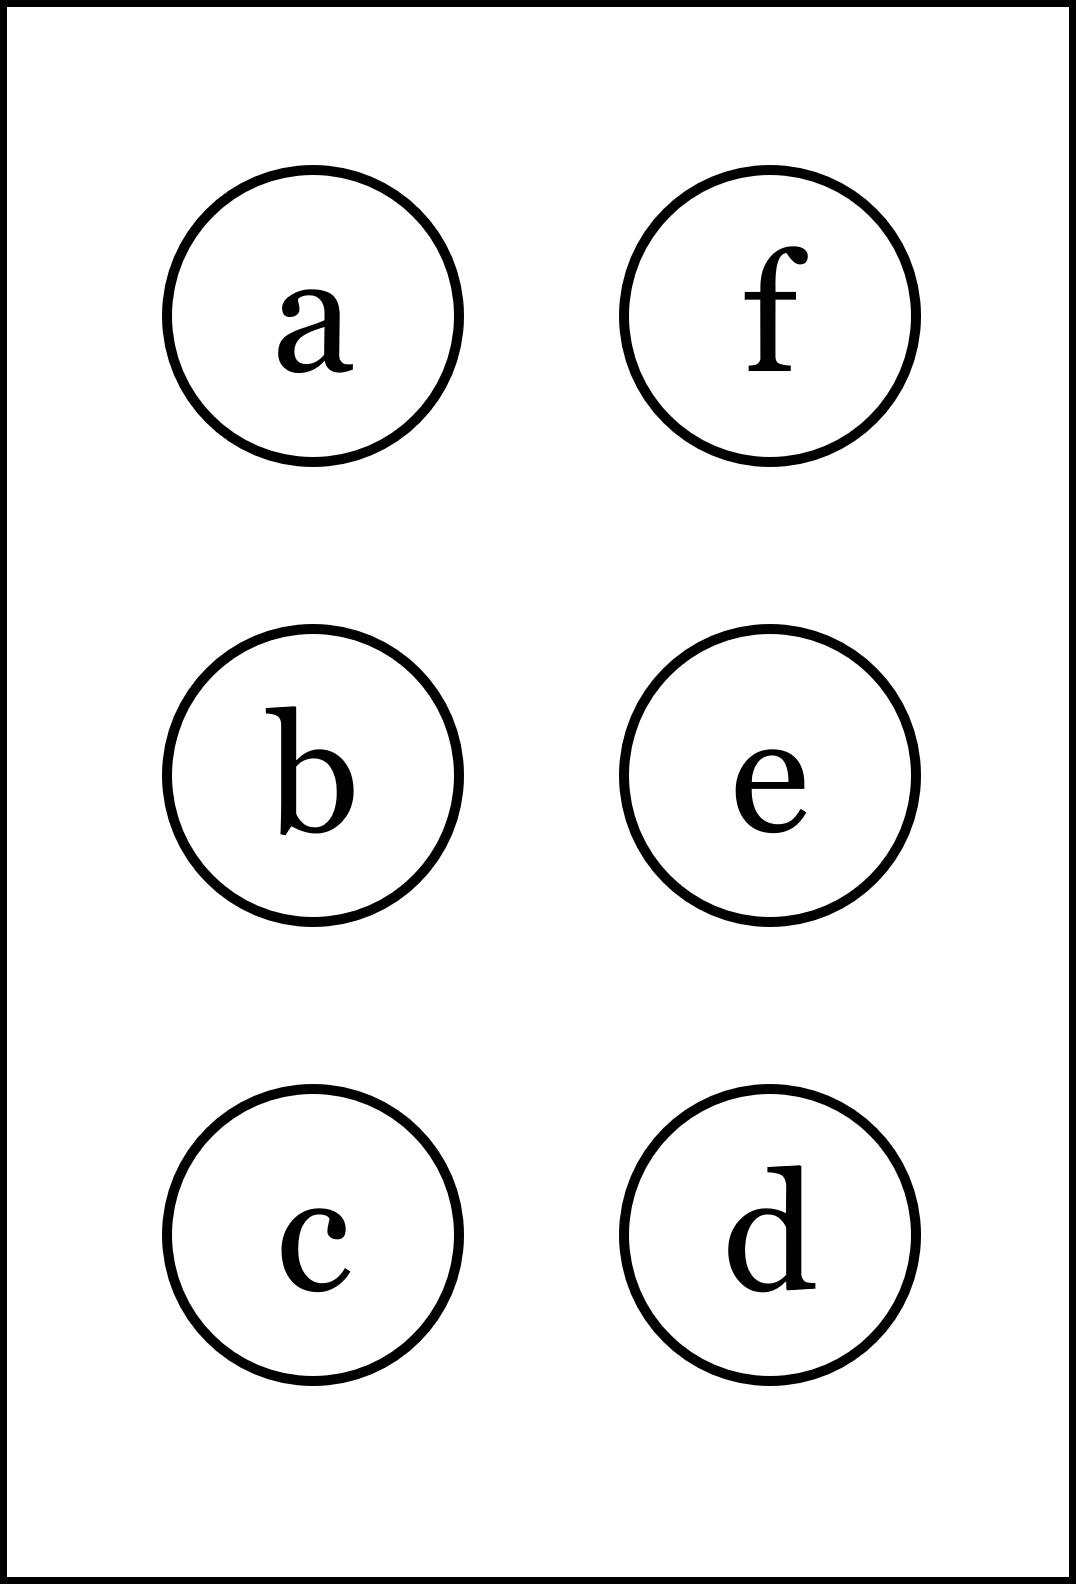
\includegraphics[height=40mm]{../images/braille.png}
{\small Písmeno Braillovej abecedy}
\end{center}
\end{minipage}
\end{center}
\end{minipage}
&
\begin{minipage}[c][104.5mm][t]{0.5\linewidth}
\begin{center}
\vspace{7mm}
{\huge Odmocniny a limity, skupina \textit{Epsilon $\epsilon$} -\romannumeral2}\\[5mm]
\textit{Jméno:}\phantom{xxxxxxxxxxxxxxxxxxxxxxxxxxxxxxxxxxxxxxxxxxxxxxxxxxxxxxxxxxxxxxxxx}\\[5mm]
\begin{minipage}{0.95\linewidth}
\begin{center}
V \textbf{(a)} a \textbf{(b)} \textbf{uprav výrazy}, v \textbf{(c)} a \textbf{(d)} \textbf{vypočítaj limity}.\\Pokud se výsledky shodujú s tými za otazníky, tak napravo obarvi\\příslušející kroužek načerno. \textbf{Spolu odevzdejte výsledné slovo}.
\end{center}
\end{minipage}
\\[1mm]
\begin{minipage}{0.79\linewidth}
\begin{center}
\begin{varwidth}{\linewidth}
\begin{enumerate}
\small
\item $\sqrt[6]{\left(\cfrac{x^{2}\;x^{2}}{x^{\nicefrac{-1}{3}}}\right)^{8}}$\quad \dotfill\; ???\;\dotfill \quad $x^{\nicefrac{52}{9}}$
\item {\footnotesize{\scriptsize$\big(\sqrt{2x+4y}+\sqrt{2x-4y}\big)^2-\big(\sqrt{2x+4y}-\sqrt{2x-4y}\big)^2$}\quad \dotfill\; ???\;\dotfill \quad $8\sqrt{x^2-2y^2}$}
\item $\lim\limits_{n\to\infty}\cfrac{n^{-1/2}}{\sqrt{64n+8}-\sqrt{64n-4}}$\quad \dotfill\; ???\;\dotfill \quad $\nicefrac{4}{3}$
\item $\lim\limits_{n\to\infty}2n\cfrac{\sqrt{n^2+n-1}-\sqrt{n^2+6}}{\sqrt{25n^2+9n-4}}$\quad \dotfill\; ???\;\dotfill \quad $\nicefrac{2}{5}$
\item \quad \dotfill\; ???\;\dotfill \quad vybarvi
\item \quad \dotfill\; ???\;\dotfill \quad nebarvi
\end{enumerate}
\end{varwidth}
\end{center}
\end{minipage}
\begin{minipage}{0.20\linewidth}
\begin{center}
{\Huge\bfseries 2.} \\[2mm]
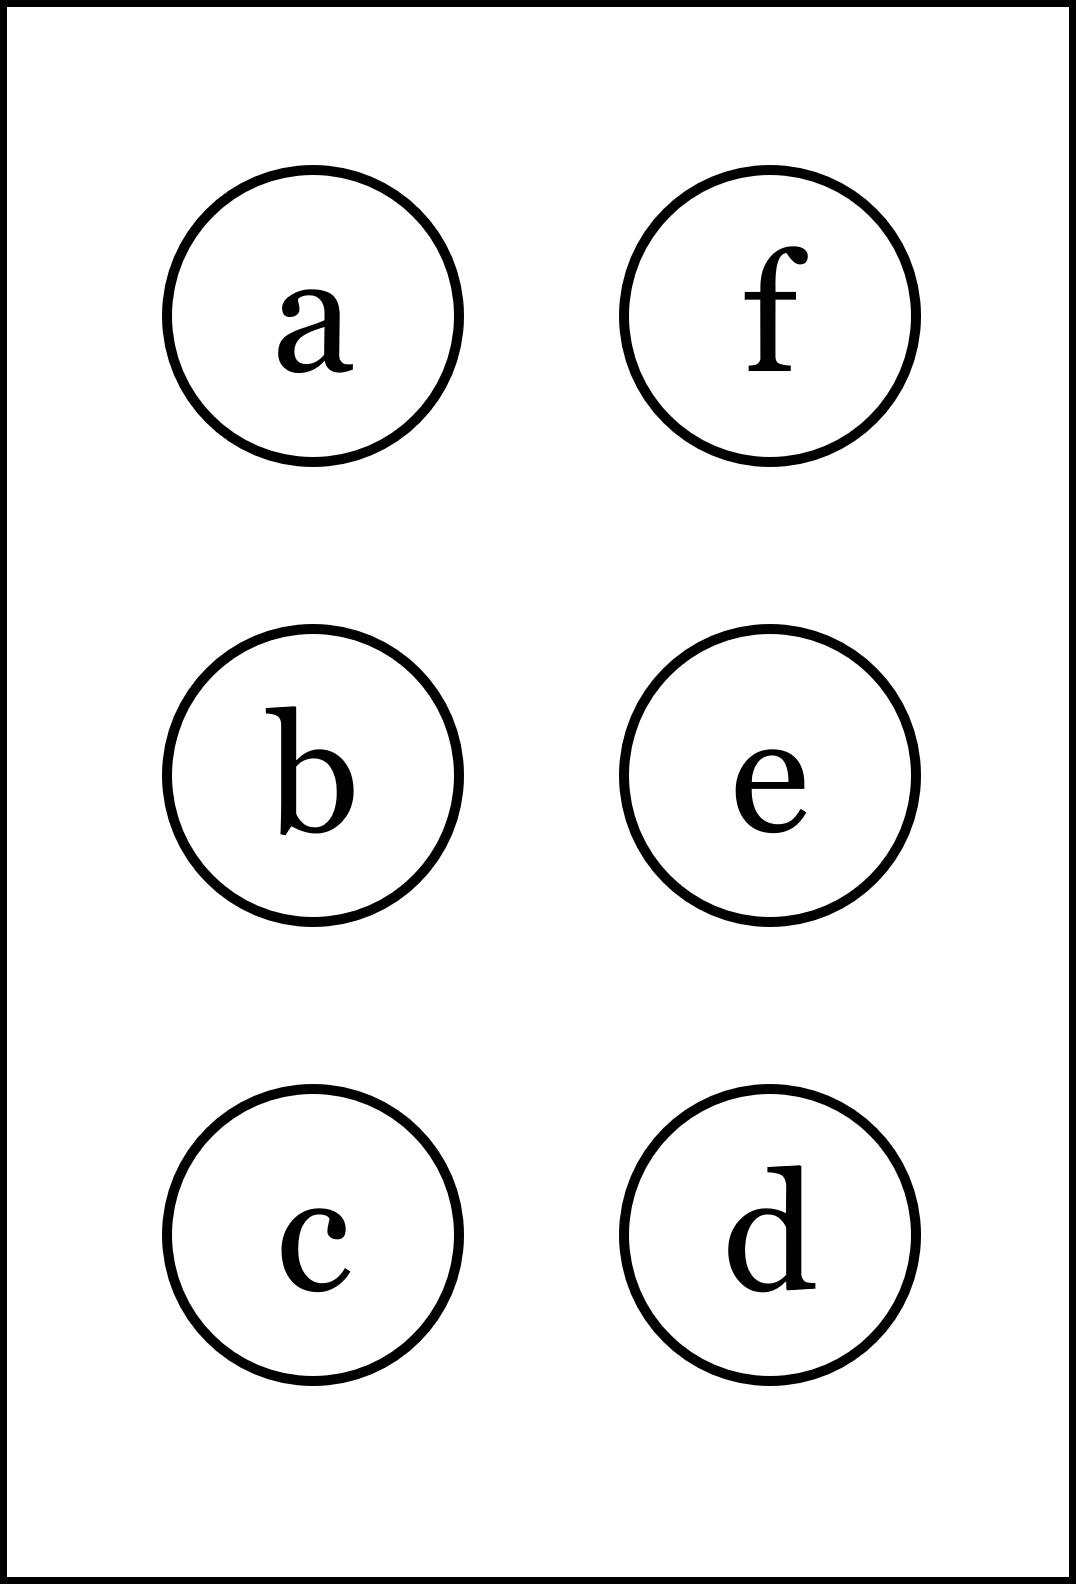
\includegraphics[height=40mm]{../images/braille.png}
{\small Písmeno Braillovej abecedy}
\end{center}
\end{minipage}
\end{center}
\end{minipage}
\\ \hdashline
\begin{minipage}[c][104.5mm][t]{0.5\linewidth}
\begin{center}
\vspace{7mm}
{\huge Odmocniny a limity, skupina \textit{Epsilon $\epsilon$} -\romannumeral3}\\[5mm]
\textit{Jméno:}\phantom{xxxxxxxxxxxxxxxxxxxxxxxxxxxxxxxxxxxxxxxxxxxxxxxxxxxxxxxxxxxxxxxxx}\\[5mm]
\begin{minipage}{0.95\linewidth}
\begin{center}
V \textbf{(a)} a \textbf{(b)} \textbf{uprav výrazy}, v \textbf{(c)} a \textbf{(d)} \textbf{vypočítaj limity}.\\Pokud se výsledky shodujú s tými za otazníky, tak napravo obarvi\\příslušející kroužek načerno. \textbf{Spolu odevzdejte výsledné slovo}.
\end{center}
\end{minipage}
\\[1mm]
\begin{minipage}{0.79\linewidth}
\begin{center}
\begin{varwidth}{\linewidth}
\begin{enumerate}
\small
\item $\sqrt[5]{\left(\cfrac{x^{2}\;x^{\nicefrac{-1}{5}}}{x^{-4}}\right)^{2}}$\quad \dotfill\; ???\;\dotfill \quad $x^{\nicefrac{58}{25}}$
\item {\footnotesize{\scriptsize$\big(\sqrt{x+4y}+\sqrt{x-4y}\big)^2-\big(\sqrt{x+4y}-\sqrt{x-4y}\big)^2$}\quad \dotfill\; ???\;\dotfill \quad $4\sqrt{x^2-16y^2}$}
\item $\lim\limits_{n\to\infty}\cfrac{n^{-1/2}}{\sqrt{25n+6}-\sqrt{25n+4}}$\quad \dotfill\; ???\;\dotfill \quad $5$
\item $\lim\limits_{n\to\infty}8n\cfrac{\sqrt{9n^2-n-2}-\sqrt{9n^2+2}}{\sqrt{4n^2-n-3}}$\quad \dotfill\; ???\;\dotfill \quad $\nicefrac{-4}{3}$
\item \quad \dotfill\; ???\;\dotfill \quad vybarvi
\item \quad \dotfill\; ???\;\dotfill \quad nebarvi
\end{enumerate}
\end{varwidth}
\end{center}
\end{minipage}
\begin{minipage}{0.20\linewidth}
\begin{center}
{\Huge\bfseries 3.} \\[2mm]
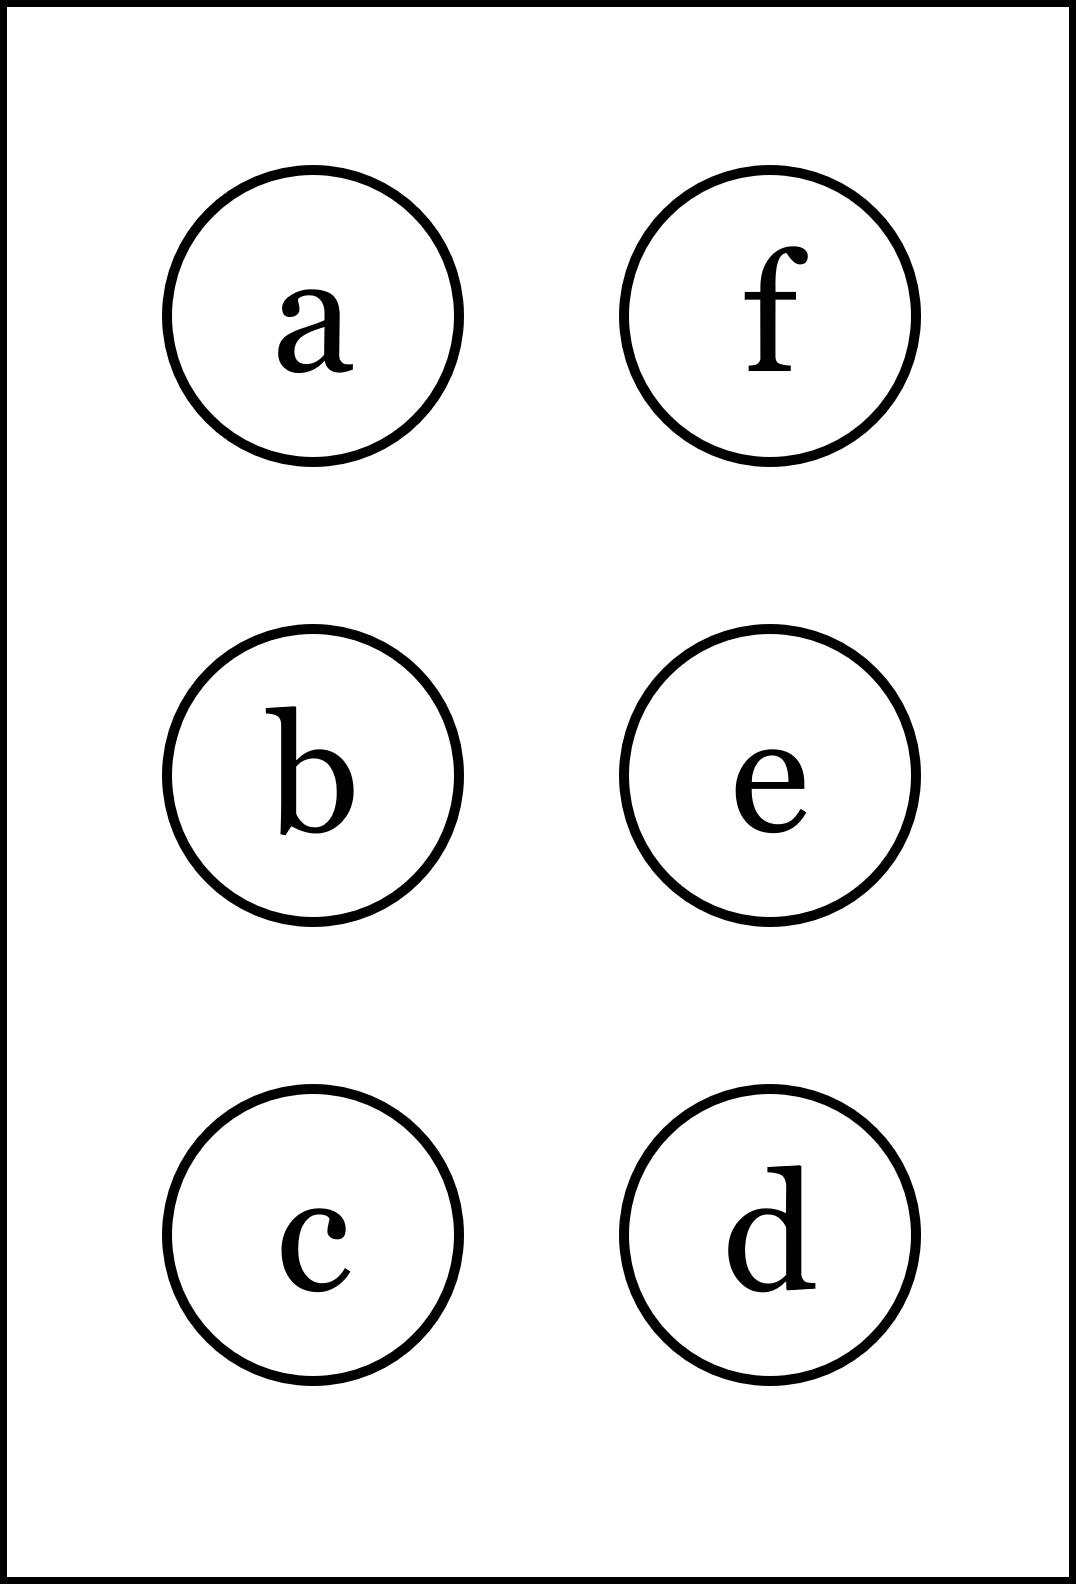
\includegraphics[height=40mm]{../images/braille.png}
{\small Písmeno Braillovej abecedy}
\end{center}
\end{minipage}
\end{center}
\end{minipage}
&
\begin{minipage}[c][104.5mm][t]{0.5\linewidth}
\begin{center}
\vspace{7mm}
{\huge Odmocniny a limity, skupina \textit{Epsilon $\epsilon$} -\romannumeral4}\\[5mm]
\textit{Jméno:}\phantom{xxxxxxxxxxxxxxxxxxxxxxxxxxxxxxxxxxxxxxxxxxxxxxxxxxxxxxxxxxxxxxxxx}\\[5mm]
\begin{minipage}{0.95\linewidth}
\begin{center}
V \textbf{(a)} a \textbf{(b)} \textbf{uprav výrazy}, v \textbf{(c)} a \textbf{(d)} \textbf{vypočítaj limity}.\\Pokud se výsledky shodujú s tými za otazníky, tak napravo obarvi\\příslušející kroužek načerno. \textbf{Spolu odevzdejte výsledné slovo}.
\end{center}
\end{minipage}
\\[1mm]
\begin{minipage}{0.79\linewidth}
\begin{center}
\begin{varwidth}{\linewidth}
\begin{enumerate}
\small
\item $\sqrt[8]{\left(\cfrac{x^{1}\;x^{5}}{x^{\nicefrac{3}{2}}}\right)^{4}}$\quad \dotfill\; ???\;\dotfill \quad $x^{\nicefrac{9}{4}}$
\item {\footnotesize{\scriptsize$\big(\sqrt{6x-12y}+\sqrt{6x+12y}\big)^2-\big(\sqrt{6x-12y}-\sqrt{6x+12y}\big)^2$}\quad \dotfill\; ???\;\dotfill \quad $24\sqrt{x^2+2y^2}$}
\item $\lim\limits_{n\to\infty}\cfrac{n^{-1/2}}{\sqrt{25n-2}-\sqrt{25n+3}}$\quad \dotfill\; ???\;\dotfill \quad $-1$
\item $\lim\limits_{n\to\infty}7n\cfrac{\sqrt{9n^2-2n+6}-\sqrt{9n^2-7}}{\sqrt{n^2+6n-3}}$\quad \dotfill\; ???\;\dotfill \quad $\nicefrac{-14}{3}$
\item \quad \dotfill\; ???\;\dotfill \quad vybarvi
\item \quad \dotfill\; ???\;\dotfill \quad vybarvi
\end{enumerate}
\end{varwidth}
\end{center}
\end{minipage}
\begin{minipage}{0.20\linewidth}
\begin{center}
{\Huge\bfseries 4.} \\[2mm]
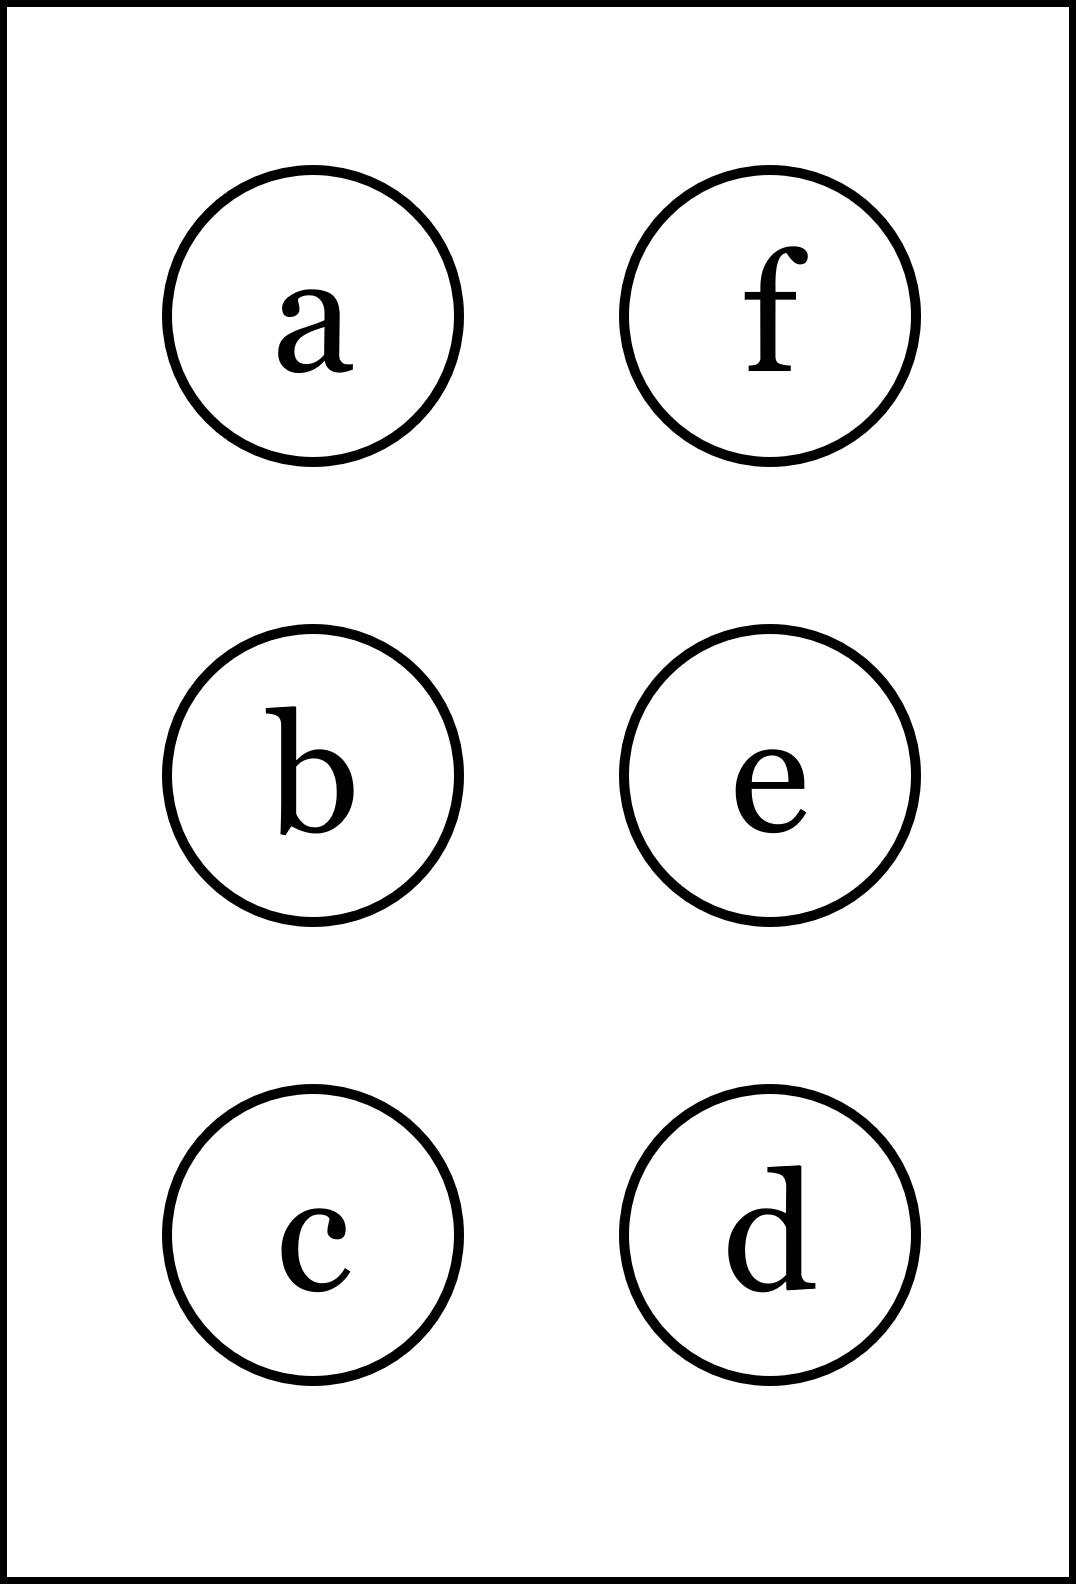
\includegraphics[height=40mm]{../images/braille.png}
{\small Písmeno Braillovej abecedy}
\end{center}
\end{minipage}
\end{center}
\end{minipage}
%
\end{tabular}
\newpage
\thispagestyle{empty}
\begin{tabular}{c:c}
\begin{minipage}[c][104.5mm][t]{0.5\linewidth}
\begin{center}
\vspace{7mm}
{\huge Odmocniny a limity, skupina \textit{Zeta $\zeta$} -\romannumeral1}\\[5mm]
\textit{Jméno:}\phantom{xxxxxxxxxxxxxxxxxxxxxxxxxxxxxxxxxxxxxxxxxxxxxxxxxxxxxxxxxxxxxxxxx}\\[5mm]
\begin{minipage}{0.95\linewidth}
\begin{center}
V \textbf{(a)} a \textbf{(b)} \textbf{uprav výrazy}, v \textbf{(c)} a \textbf{(d)} \textbf{vypočítaj limity}.\\Pokud se výsledky shodujú s tými za otazníky, tak napravo obarvi\\příslušející kroužek načerno. \textbf{Spolu odevzdejte výsledné slovo}.
\end{center}
\end{minipage}
\\[1mm]
\begin{minipage}{0.79\linewidth}
\begin{center}
\begin{varwidth}{\linewidth}
\begin{enumerate}
\small
\item $\sqrt[5]{\left(\cfrac{x^{-2}\;x^{-3}}{x^{\nicefrac{-1}{2}}}\right)^{7}}$\quad \dotfill\; ???\;\dotfill \quad $x^{\nicefrac{-63}{10}}$
\item {\footnotesize{\scriptsize$\big(\sqrt{x-y}+\sqrt{x+y}\big)^2-\big(\sqrt{x-y}-\sqrt{x+y}\big)^2$}\quad \dotfill\; ???\;\dotfill \quad $4\sqrt{x^2+y^2}$}
\item $\lim\limits_{n\to\infty}\cfrac{n^{-1/2}}{\sqrt{36n-6}-\sqrt{36n-4}}$\quad \dotfill\; ???\;\dotfill \quad $\nicefrac{-6}{5}$
\item $\lim\limits_{n\to\infty}5n\cfrac{\sqrt{25n^2-n-6}-\sqrt{25n^2+5}}{\sqrt{n^2+3n+3}}$\quad \dotfill\; ???\;\dotfill \quad $-1$
\item \quad \dotfill\; ???\;\dotfill \quad vybarvi
\item \quad \dotfill\; ???\;\dotfill \quad vybarvi
\end{enumerate}
\end{varwidth}
\end{center}
\end{minipage}
\begin{minipage}{0.20\linewidth}
\begin{center}
{\Huge\bfseries 1.} \\[2mm]
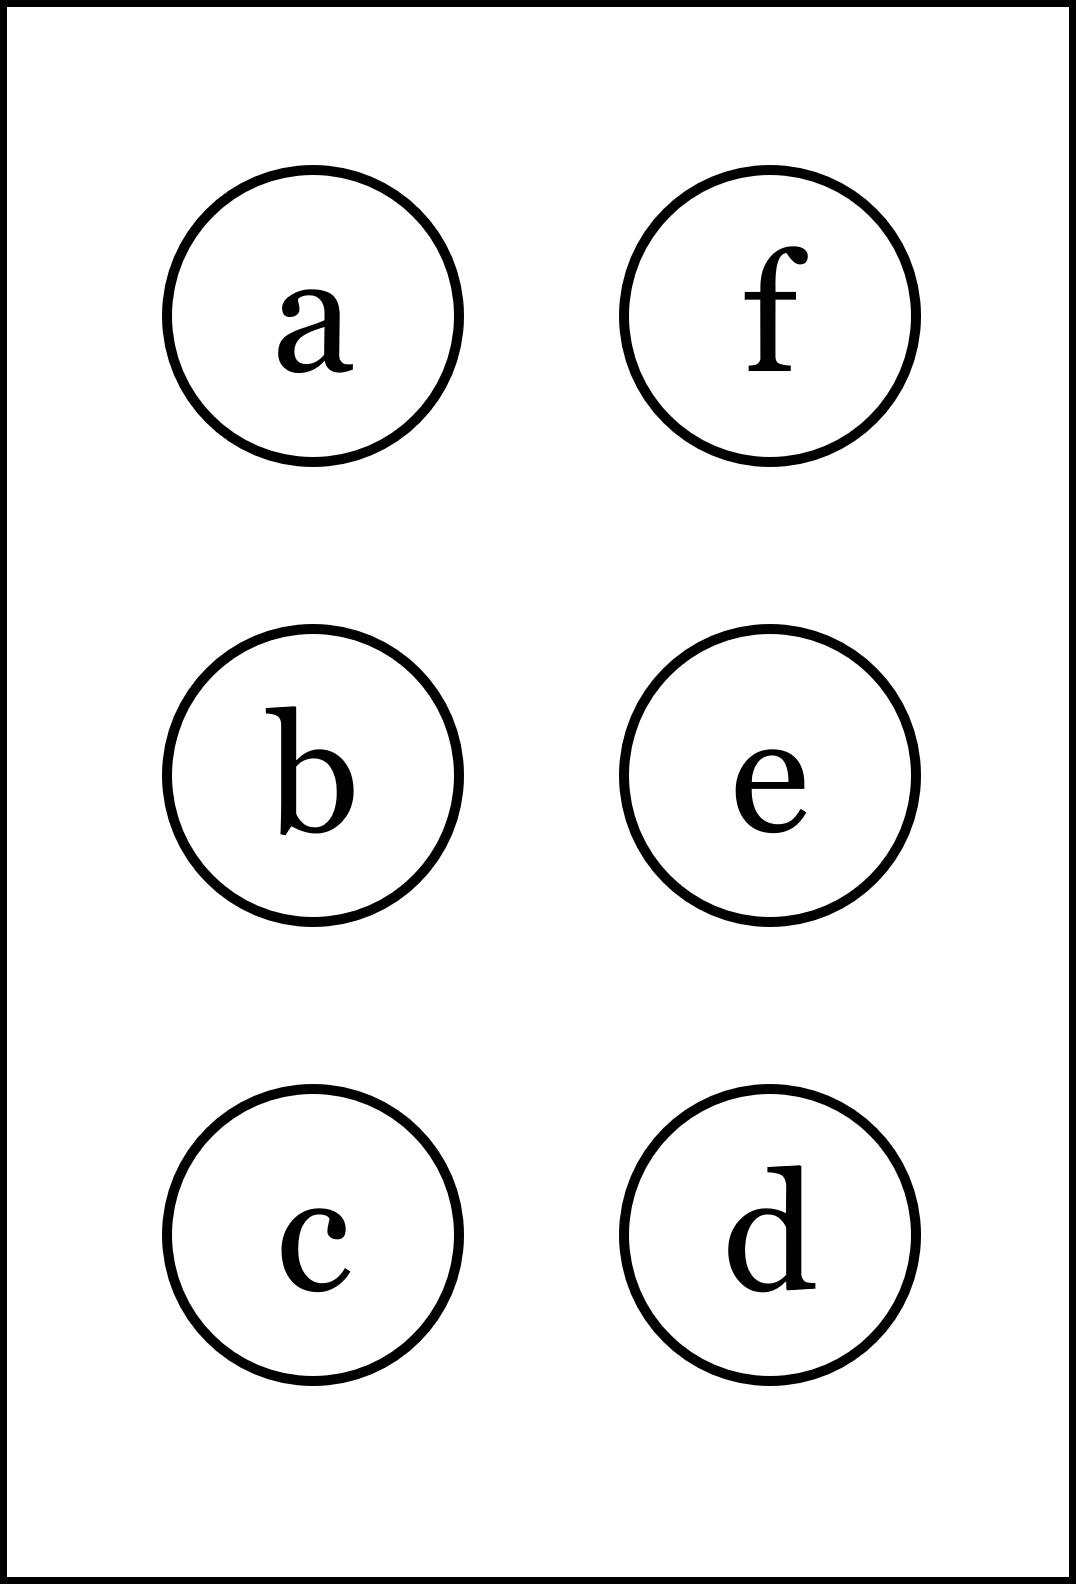
\includegraphics[height=40mm]{../images/braille.png}
{\small Písmeno Braillovej abecedy}
\end{center}
\end{minipage}
\end{center}
\end{minipage}
&
\begin{minipage}[c][104.5mm][t]{0.5\linewidth}
\begin{center}
\vspace{7mm}
{\huge Odmocniny a limity, skupina \textit{Zeta $\zeta$} -\romannumeral2}\\[5mm]
\textit{Jméno:}\phantom{xxxxxxxxxxxxxxxxxxxxxxxxxxxxxxxxxxxxxxxxxxxxxxxxxxxxxxxxxxxxxxxxx}\\[5mm]
\begin{minipage}{0.95\linewidth}
\begin{center}
V \textbf{(a)} a \textbf{(b)} \textbf{uprav výrazy}, v \textbf{(c)} a \textbf{(d)} \textbf{vypočítaj limity}.\\Pokud se výsledky shodujú s tými za otazníky, tak napravo obarvi\\příslušející kroužek načerno. \textbf{Spolu odevzdejte výsledné slovo}.
\end{center}
\end{minipage}
\\[1mm]
\begin{minipage}{0.79\linewidth}
\begin{center}
\begin{varwidth}{\linewidth}
\begin{enumerate}
\small
\item $\sqrt[1]{\left(\cfrac{x^{6}\;x^{4}}{x^{\nicefrac{-3}{2}}}\right)^{2}}$\quad \dotfill\; ???\;\dotfill \quad $x^{23}$
\item {\footnotesize{\scriptsize$\big(\sqrt{2x-8y}+\sqrt{2x+8y}\big)^2-\big(\sqrt{2x-8y}-\sqrt{2x+8y}\big)^2$}\quad \dotfill\; ???\;\dotfill \quad $8\sqrt{x^2-16y^2}$}
\item $\lim\limits_{n\to\infty}\cfrac{n^{-1/2}}{\sqrt{64n+5}-\sqrt{64n+6}}$\quad \dotfill\; ???\;\dotfill \quad $-16$
\item $\lim\limits_{n\to\infty}3n\cfrac{\sqrt{9n^2-n-6}-\sqrt{9n^2-3}}{\sqrt{n^2+n-7}}$\quad \dotfill\; ???\;\dotfill \quad $-1$
\item \quad \dotfill\; ???\;\dotfill \quad vybarvi
\item \quad \dotfill\; ???\;\dotfill \quad nebarvi
\end{enumerate}
\end{varwidth}
\end{center}
\end{minipage}
\begin{minipage}{0.20\linewidth}
\begin{center}
{\Huge\bfseries 2.} \\[2mm]
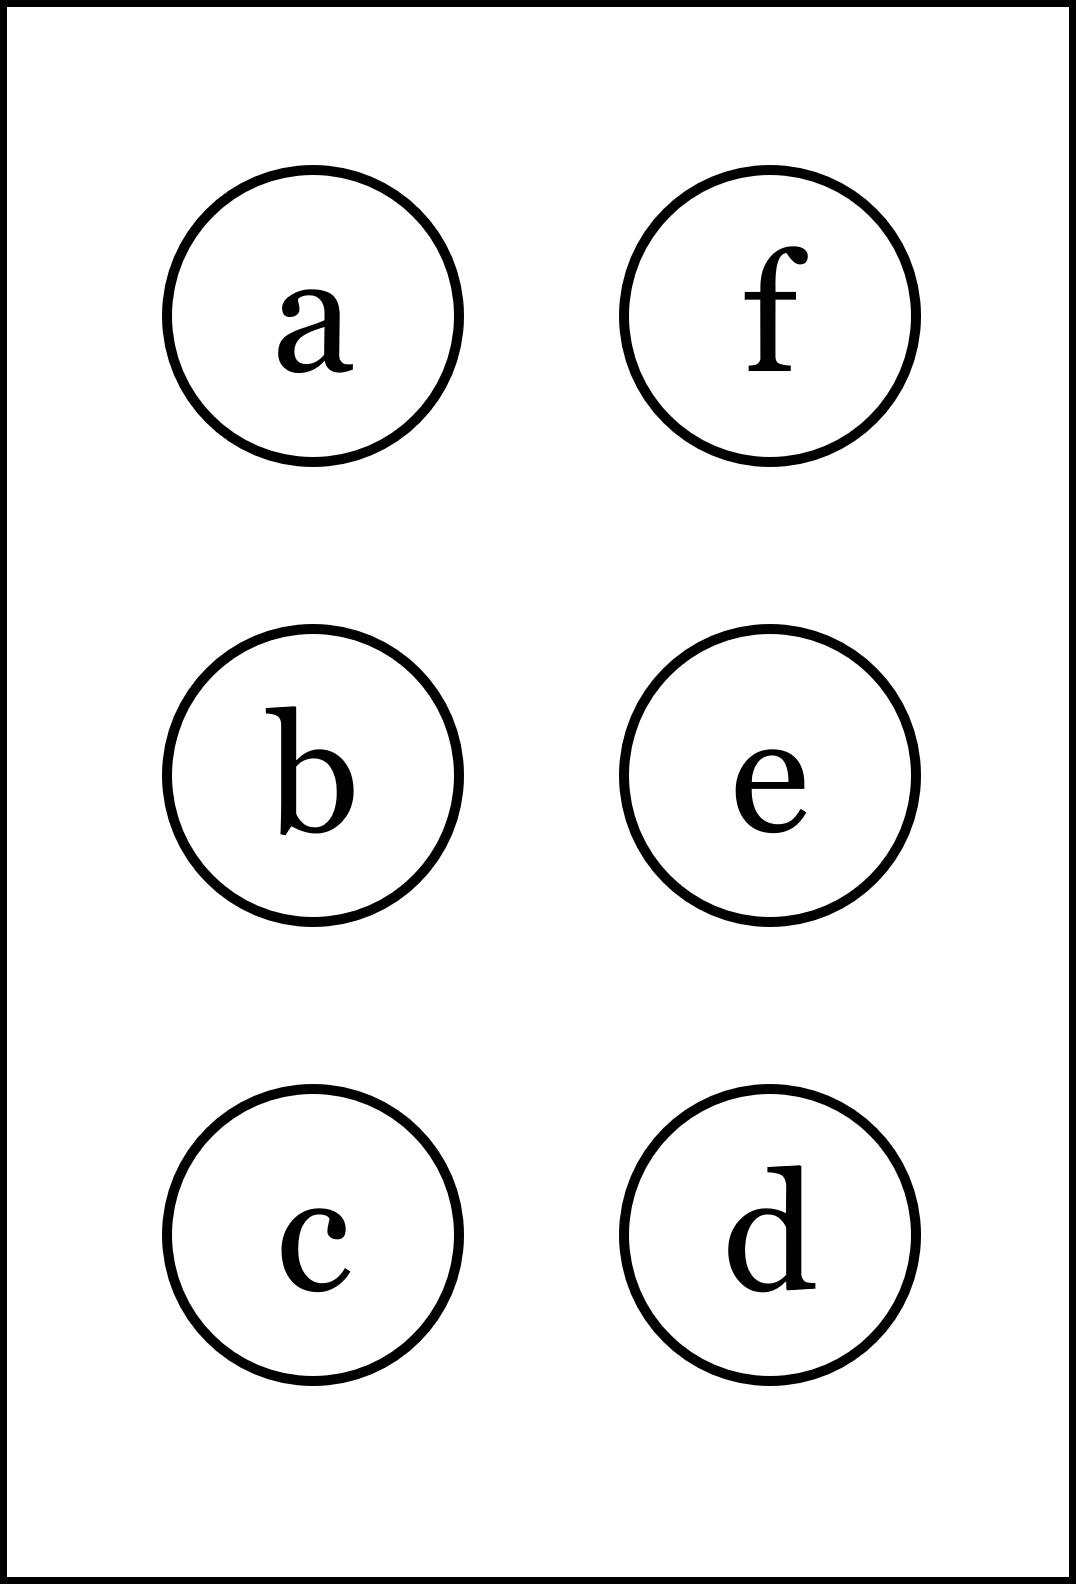
\includegraphics[height=40mm]{../images/braille.png}
{\small Písmeno Braillovej abecedy}
\end{center}
\end{minipage}
\end{center}
\end{minipage}
\\ \hdashline
\begin{minipage}[c][104.5mm][t]{0.5\linewidth}
\begin{center}
\vspace{7mm}
{\huge Odmocniny a limity, skupina \textit{Zeta $\zeta$} -\romannumeral3}\\[5mm]
\textit{Jméno:}\phantom{xxxxxxxxxxxxxxxxxxxxxxxxxxxxxxxxxxxxxxxxxxxxxxxxxxxxxxxxxxxxxxxxx}\\[5mm]
\begin{minipage}{0.95\linewidth}
\begin{center}
V \textbf{(a)} a \textbf{(b)} \textbf{uprav výrazy}, v \textbf{(c)} a \textbf{(d)} \textbf{vypočítaj limity}.\\Pokud se výsledky shodujú s tými za otazníky, tak napravo obarvi\\příslušející kroužek načerno. \textbf{Spolu odevzdejte výsledné slovo}.
\end{center}
\end{minipage}
\\[1mm]
\begin{minipage}{0.79\linewidth}
\begin{center}
\begin{varwidth}{\linewidth}
\begin{enumerate}
\small
\item $\sqrt[1]{\left(\cfrac{x^{2}\;x^{-1}}{x^{1}}\right)^{3}}$\quad \dotfill\; ???\;\dotfill \quad $x^{0}$
\item {\footnotesize{\scriptsize$\big(\sqrt{4x-8y}+\sqrt{4x+8y}\big)^2-\big(\sqrt{4x-8y}-\sqrt{4x+8y}\big)^2$}\quad \dotfill\; ???\;\dotfill \quad $16\sqrt{x^2+2y^2}$}
\item $\lim\limits_{n\to\infty}\cfrac{n^{-1/2}}{\sqrt{n-2}-\sqrt{n+9}}$\quad \dotfill\; ???\;\dotfill \quad $\infty$
\item $\lim\limits_{n\to\infty}2n\cfrac{\sqrt{9n^2-3n-1}-\sqrt{9n^2+4}}{\sqrt{n^2-n+6}}$\quad \dotfill\; ???\;\dotfill \quad $-2$
\item \quad \dotfill\; ???\;\dotfill \quad nebarvi
\item \quad \dotfill\; ???\;\dotfill \quad nebarvi
\end{enumerate}
\end{varwidth}
\end{center}
\end{minipage}
\begin{minipage}{0.20\linewidth}
\begin{center}
{\Huge\bfseries 3.} \\[2mm]
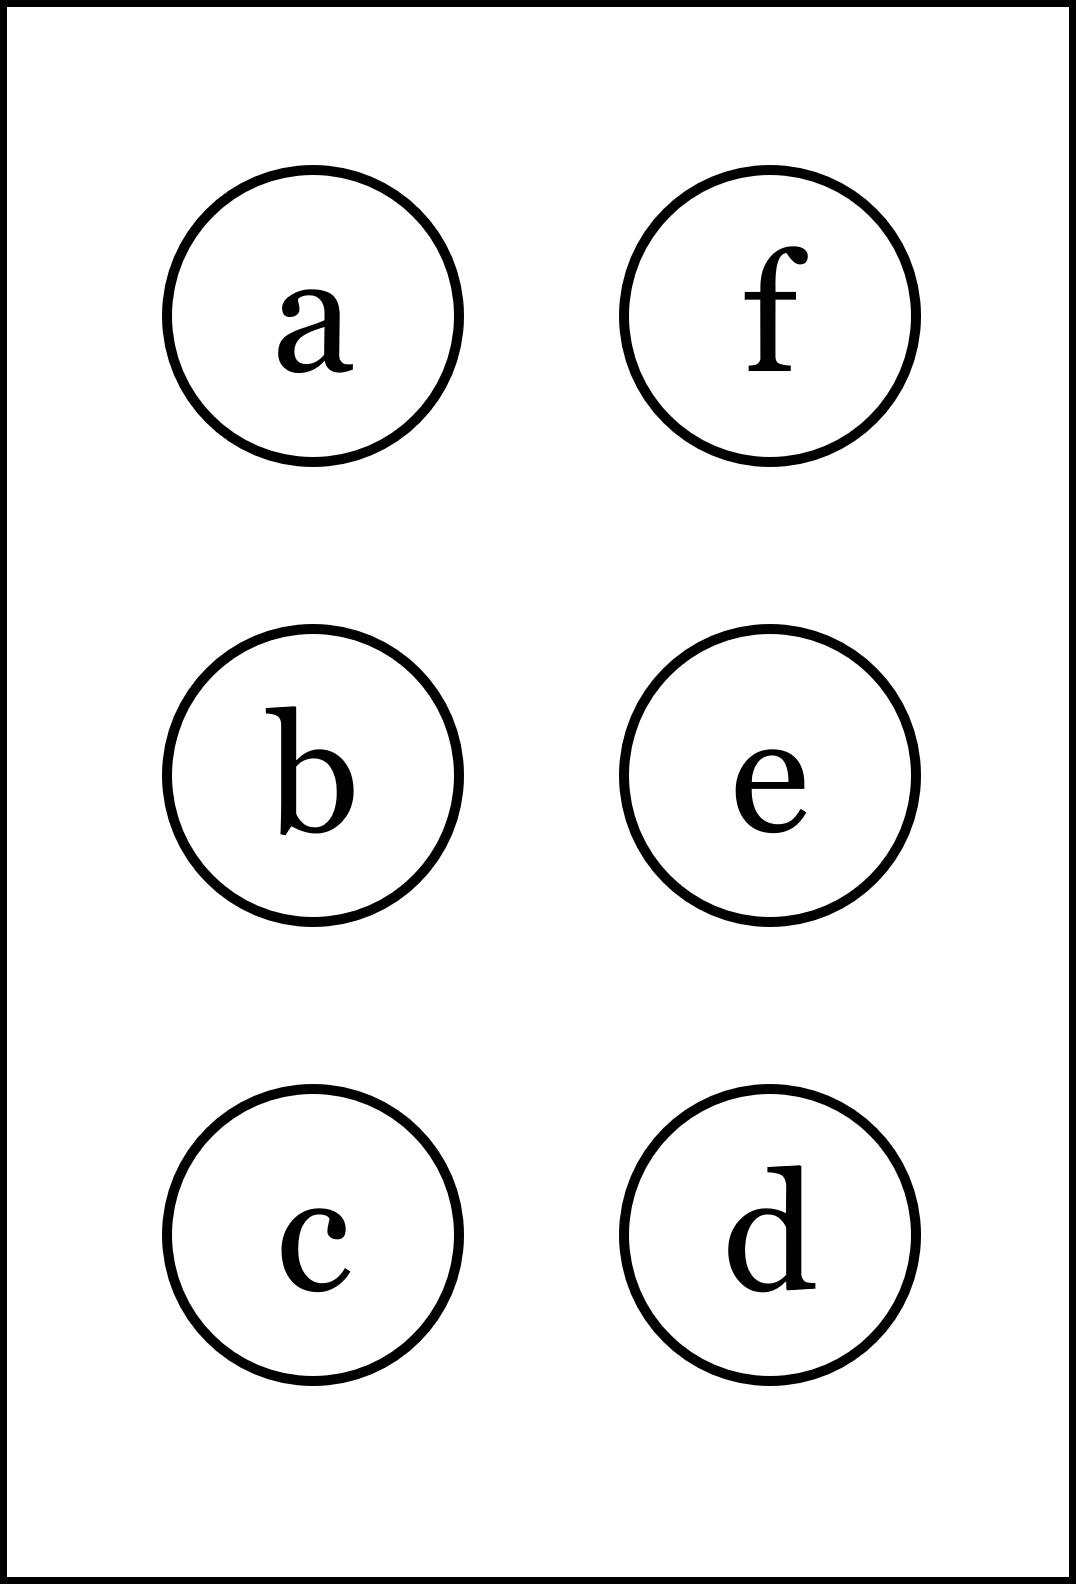
\includegraphics[height=40mm]{../images/braille.png}
{\small Písmeno Braillovej abecedy}
\end{center}
\end{minipage}
\end{center}
\end{minipage}
&
\begin{minipage}[c][104.5mm][t]{0.5\linewidth}
\begin{center}
\vspace{7mm}
{\huge Odmocniny a limity, skupina \textit{Zeta $\zeta$} -\romannumeral4}\\[5mm]
\textit{Jméno:}\phantom{xxxxxxxxxxxxxxxxxxxxxxxxxxxxxxxxxxxxxxxxxxxxxxxxxxxxxxxxxxxxxxxxx}\\[5mm]
\begin{minipage}{0.95\linewidth}
\begin{center}
V \textbf{(a)} a \textbf{(b)} \textbf{uprav výrazy}, v \textbf{(c)} a \textbf{(d)} \textbf{vypočítaj limity}.\\Pokud se výsledky shodujú s tými za otazníky, tak napravo obarvi\\příslušející kroužek načerno. \textbf{Spolu odevzdejte výsledné slovo}.
\end{center}
\end{minipage}
\\[1mm]
\begin{minipage}{0.79\linewidth}
\begin{center}
\begin{varwidth}{\linewidth}
\begin{enumerate}
\small
\item $\sqrt[1]{\left(\cfrac{x^{\nicefrac{-1}{3}}\;x^{\nicefrac{3}{4}}}{x^{1}}\right)^{2}}$\quad \dotfill\; ???\;\dotfill \quad $x^{\nicefrac{-7}{6}}$
\item {\footnotesize{\scriptsize$\big(\sqrt{3x+9y}+\sqrt{3x-9y}\big)^2-\big(\sqrt{3x+9y}-\sqrt{3x-9y}\big)^2$}\quad \dotfill\; ???\;\dotfill \quad $12\sqrt{x^2-3y^2}$}
\item $\lim\limits_{n\to\infty}\cfrac{n^{-1/2}}{\sqrt{n-3}-\sqrt{n+6}}$\quad \dotfill\; ???\;\dotfill \quad $\nicefrac{-2}{9}$
\item $\lim\limits_{n\to\infty}9n\cfrac{\sqrt{n^2+7n+4}-\sqrt{n^2-4}}{\sqrt{4n^2-n-4}}$\quad \dotfill\; ???\;\dotfill \quad $\nicefrac{63}{2}$
\item \quad \dotfill\; ???\;\dotfill \quad nebarvi
\item \quad \dotfill\; ???\;\dotfill \quad nebarvi
\end{enumerate}
\end{varwidth}
\end{center}
\end{minipage}
\begin{minipage}{0.20\linewidth}
\begin{center}
{\Huge\bfseries 4.} \\[2mm]
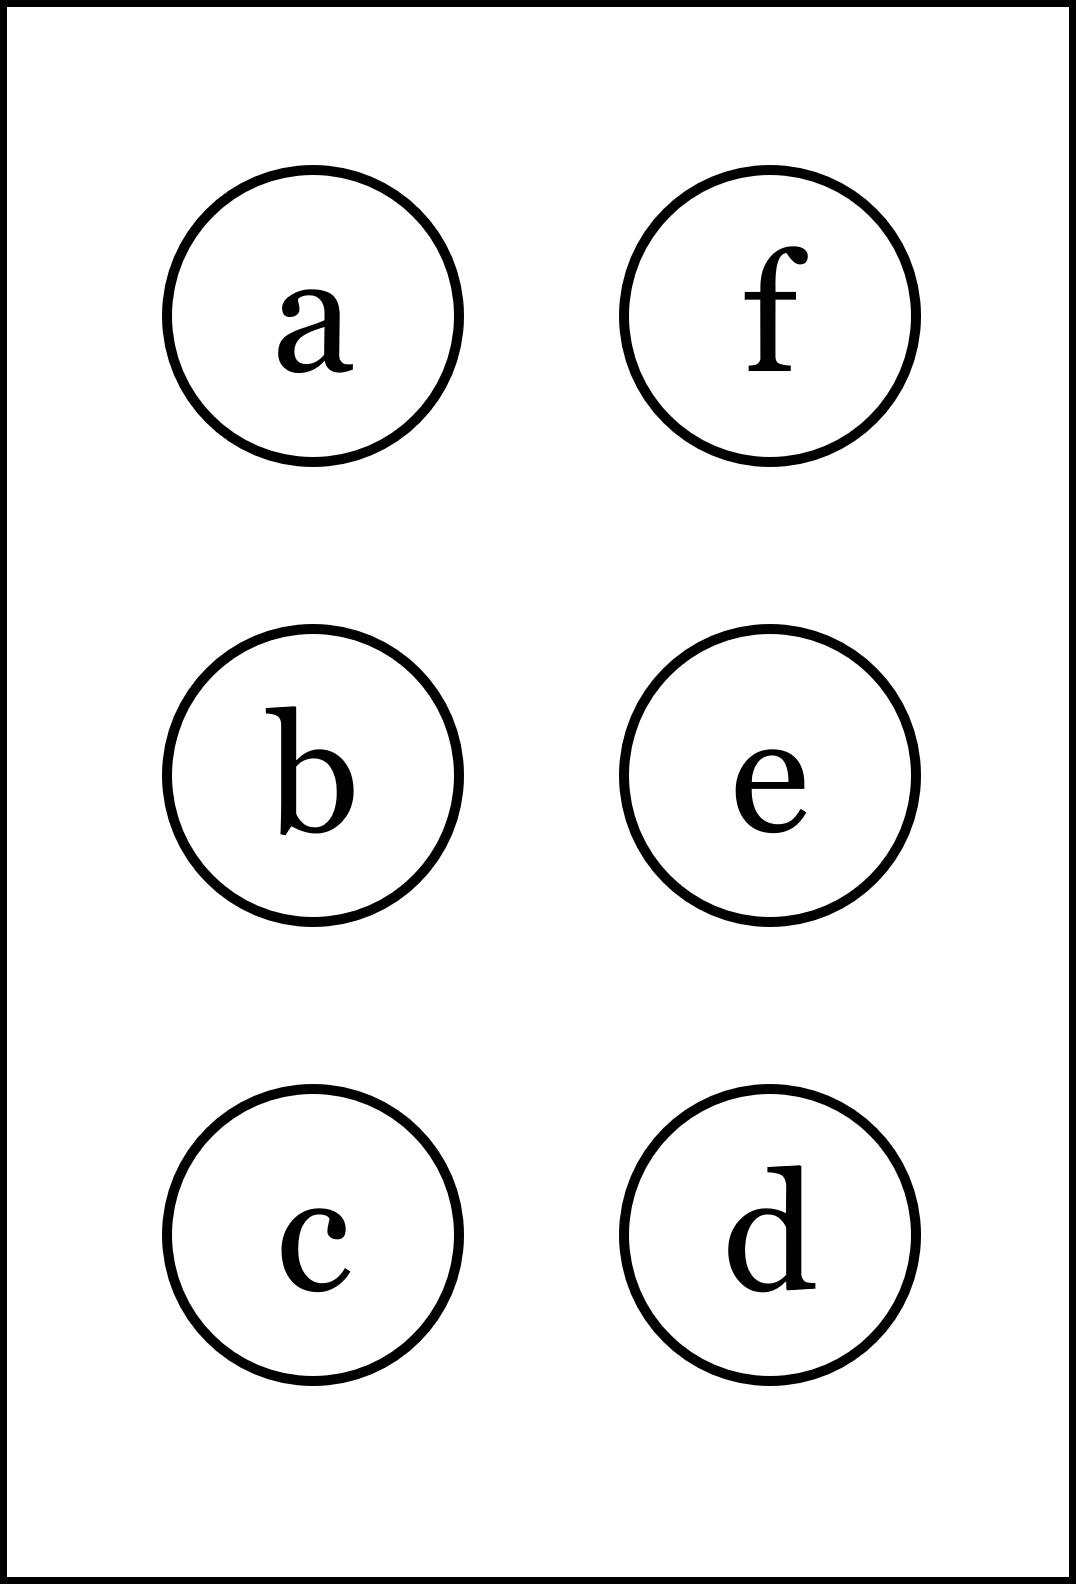
\includegraphics[height=40mm]{../images/braille.png}
{\small Písmeno Braillovej abecedy}
\end{center}
\end{minipage}
\end{center}
\end{minipage}
%
\end{tabular}
\newpage
\thispagestyle{empty}
\begin{tabular}{c:c}
\begin{minipage}[c][104.5mm][t]{0.5\linewidth}
\begin{center}
\vspace{7mm}
{\huge Odmocniny a limity, skupina \textit{Eta $\eta$} -\romannumeral1}\\[5mm]
\textit{Jméno:}\phantom{xxxxxxxxxxxxxxxxxxxxxxxxxxxxxxxxxxxxxxxxxxxxxxxxxxxxxxxxxxxxxxxxx}\\[5mm]
\begin{minipage}{0.95\linewidth}
\begin{center}
V \textbf{(a)} a \textbf{(b)} \textbf{uprav výrazy}, v \textbf{(c)} a \textbf{(d)} \textbf{vypočítaj limity}.\\Pokud se výsledky shodujú s tými za otazníky, tak napravo obarvi\\příslušející kroužek načerno. \textbf{Spolu odevzdejte výsledné slovo}.
\end{center}
\end{minipage}
\\[1mm]
\begin{minipage}{0.79\linewidth}
\begin{center}
\begin{varwidth}{\linewidth}
\begin{enumerate}
\small
\item $\sqrt[3]{\left(\cfrac{x^{-2}\;x^{-6}}{x^{-1}}\right)^{2}}$\quad \dotfill\; ???\;\dotfill \quad $x^{\nicefrac{10}{3}}$
\item {\footnotesize{\scriptsize$\big(\sqrt{x+8y}+\sqrt{x-8y}\big)^2-\big(\sqrt{x+8y}-\sqrt{x-8y}\big)^2$}\quad \dotfill\; ???\;\dotfill \quad $4\sqrt{x^2-64y^2}$}
\item $\lim\limits_{n\to\infty}\cfrac{n^{-1/2}}{\sqrt{64n-4}-\sqrt{64n-2}}$\quad \dotfill\; ???\;\dotfill \quad $-8$
\item $\lim\limits_{n\to\infty}2n\cfrac{\sqrt{36n^2+3n+1}-\sqrt{36n^2+4}}{\sqrt{4n^2-3n+1}}$\quad \dotfill\; ???\;\dotfill \quad $\nicefrac{1}{2}$
\item \quad \dotfill\; ???\;\dotfill \quad nebarvi
\item \quad \dotfill\; ???\;\dotfill \quad vybarvi
\end{enumerate}
\end{varwidth}
\end{center}
\end{minipage}
\begin{minipage}{0.20\linewidth}
\begin{center}
{\Huge\bfseries 1.} \\[2mm]
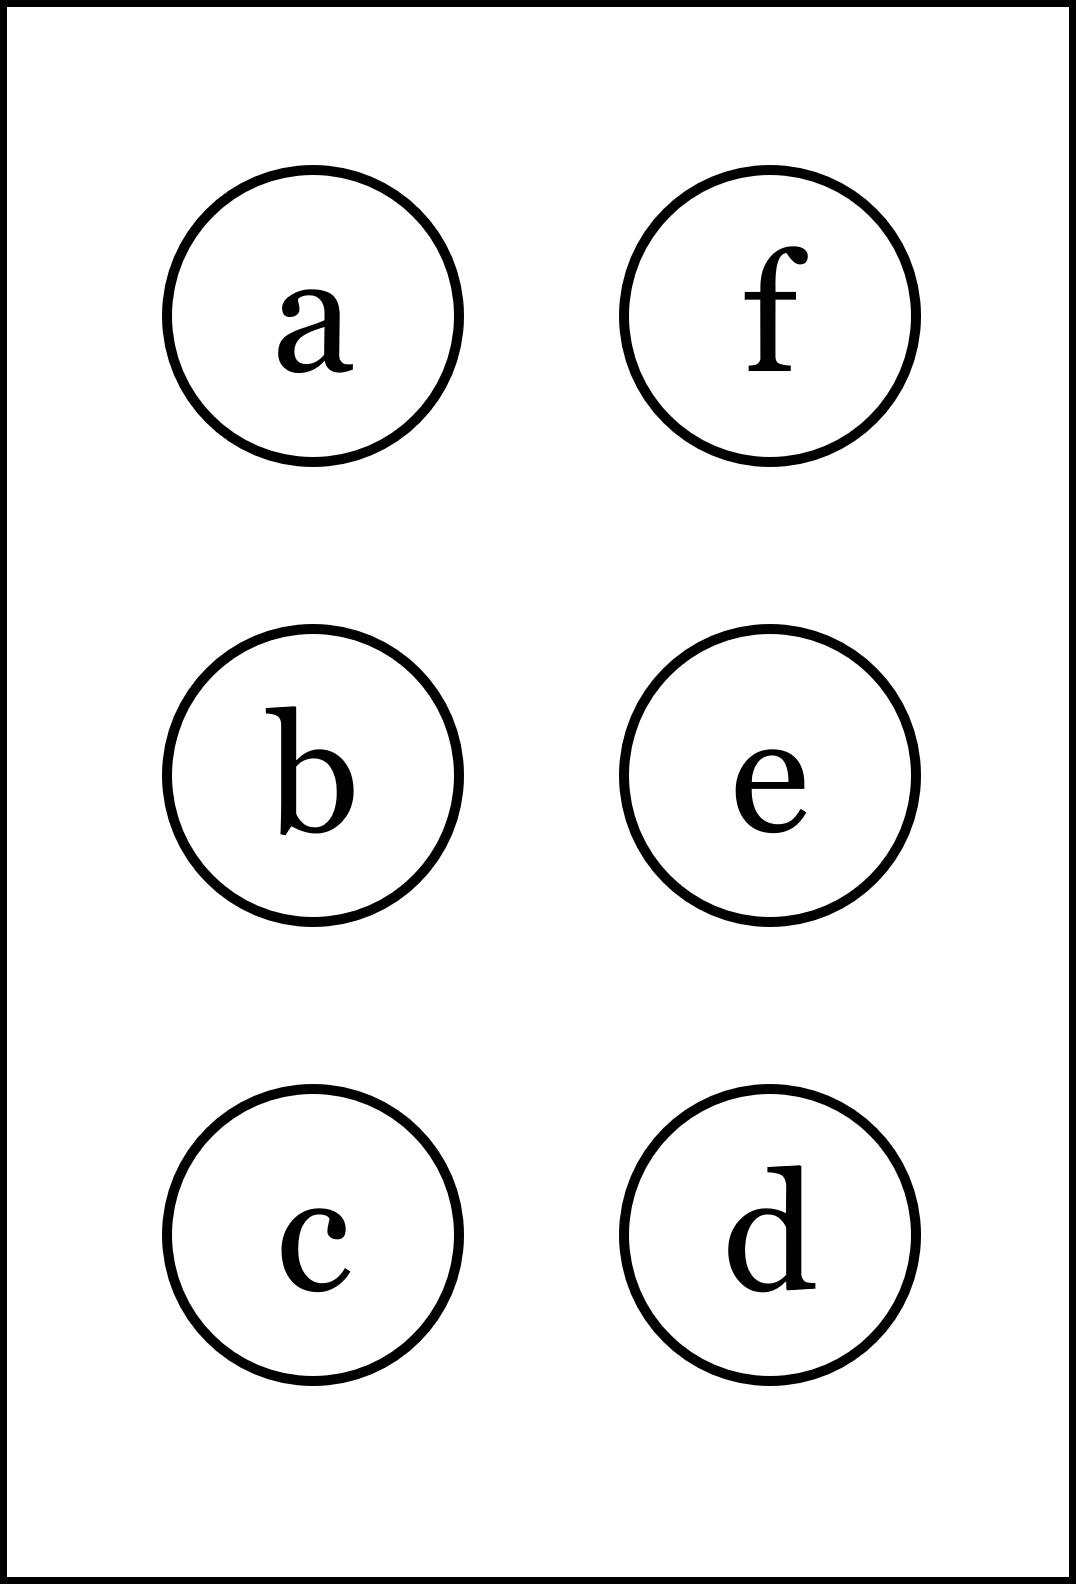
\includegraphics[height=40mm]{../images/braille.png}
{\small Písmeno Braillovej abecedy}
\end{center}
\end{minipage}
\end{center}
\end{minipage}
&
\begin{minipage}[c][104.5mm][t]{0.5\linewidth}
\begin{center}
\vspace{7mm}
{\huge Odmocniny a limity, skupina \textit{Eta $\eta$} -\romannumeral2}\\[5mm]
\textit{Jméno:}\phantom{xxxxxxxxxxxxxxxxxxxxxxxxxxxxxxxxxxxxxxxxxxxxxxxxxxxxxxxxxxxxxxxxx}\\[5mm]
\begin{minipage}{0.95\linewidth}
\begin{center}
V \textbf{(a)} a \textbf{(b)} \textbf{uprav výrazy}, v \textbf{(c)} a \textbf{(d)} \textbf{vypočítaj limity}.\\Pokud se výsledky shodujú s tými za otazníky, tak napravo obarvi\\příslušející kroužek načerno. \textbf{Spolu odevzdejte výsledné slovo}.
\end{center}
\end{minipage}
\\[1mm]
\begin{minipage}{0.79\linewidth}
\begin{center}
\begin{varwidth}{\linewidth}
\begin{enumerate}
\small
\item $\sqrt[1]{\left(\cfrac{x^{4}\;x^{5}}{x^{\nicefrac{5}{3}}}\right)^{5}}$\quad \dotfill\; ???\;\dotfill \quad $x^{\nicefrac{110}{3}}$
\item {\footnotesize{\scriptsize$\big(\sqrt{2x-8y}+\sqrt{2x+8y}\big)^2-\big(\sqrt{2x-8y}-\sqrt{2x+8y}\big)^2$}\quad \dotfill\; ???\;\dotfill \quad $8\sqrt{x^2+4y^2}$}
\item $\lim\limits_{n\to\infty}\cfrac{n^{-1/2}}{\sqrt{4n+1}-\sqrt{4n-3}}$\quad \dotfill\; ???\;\dotfill \quad $-\infty$
\item $\lim\limits_{n\to\infty}2n\cfrac{\sqrt{16n^2+2n+5}-\sqrt{16n^2+3}}{\sqrt{4n^2-2n-3}}$\quad \dotfill\; ???\;\dotfill \quad $\nicefrac{1}{2}$
\item \quad \dotfill\; ???\;\dotfill \quad vybarvi
\item \quad \dotfill\; ???\;\dotfill \quad nebarvi
\end{enumerate}
\end{varwidth}
\end{center}
\end{minipage}
\begin{minipage}{0.20\linewidth}
\begin{center}
{\Huge\bfseries 2.} \\[2mm]
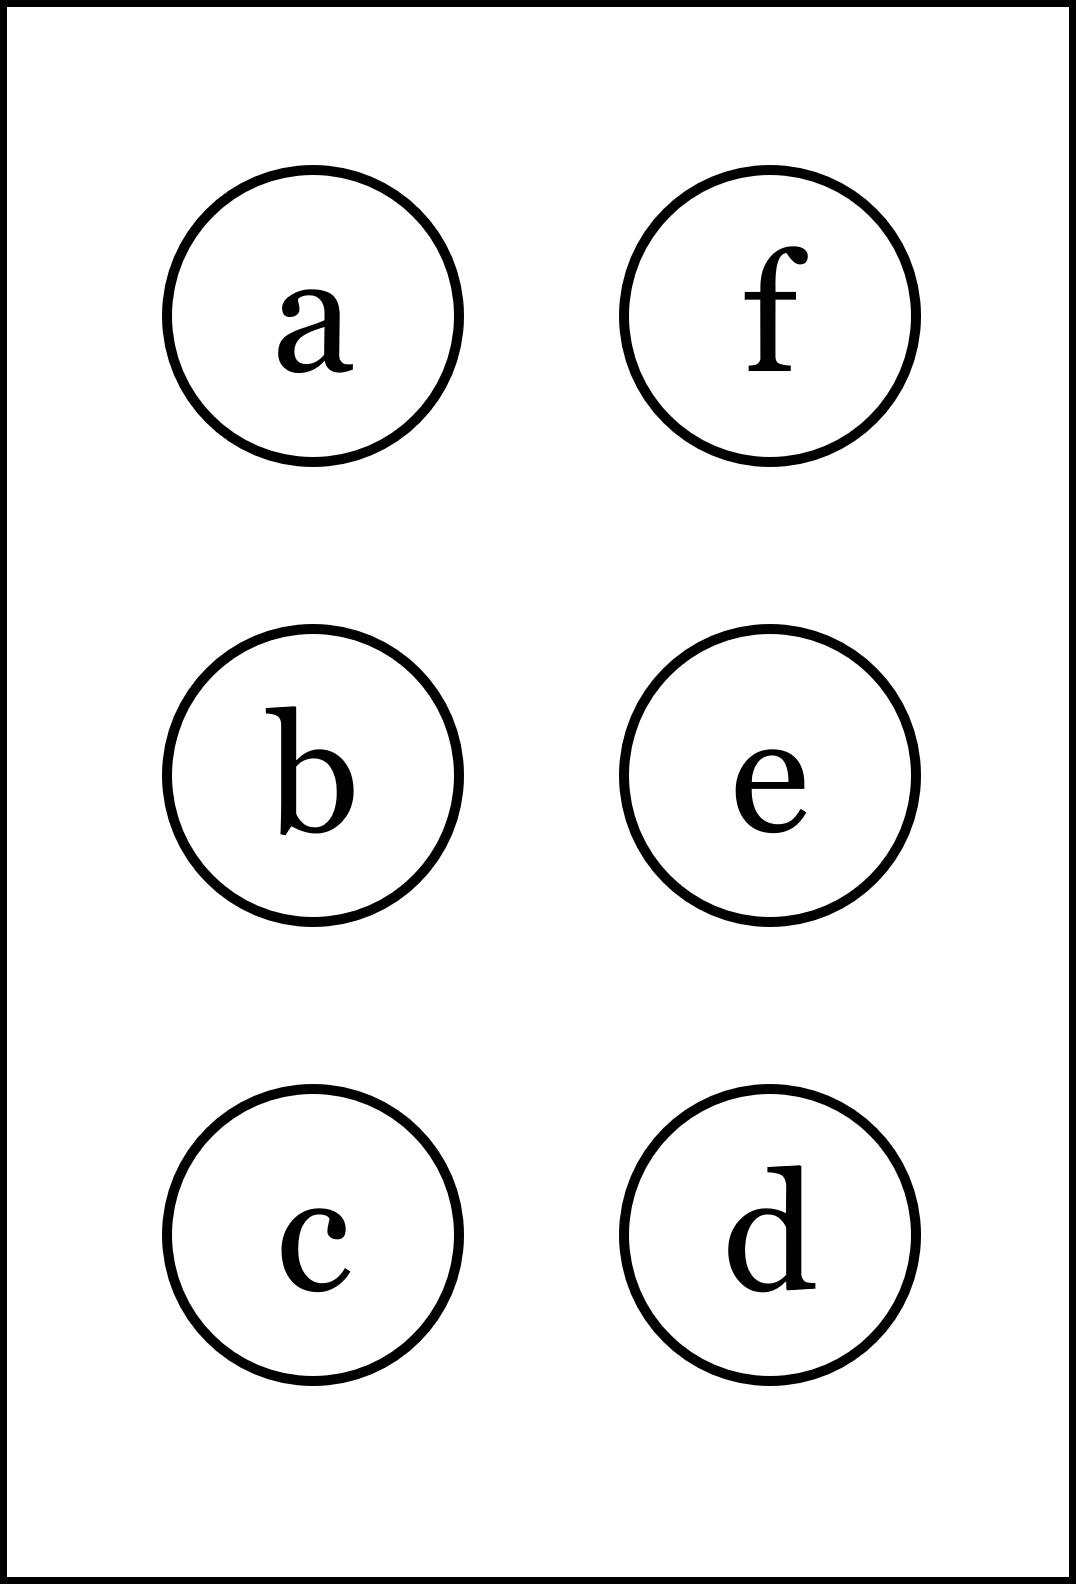
\includegraphics[height=40mm]{../images/braille.png}
{\small Písmeno Braillovej abecedy}
\end{center}
\end{minipage}
\end{center}
\end{minipage}
\\ \hdashline
\begin{minipage}[c][104.5mm][t]{0.5\linewidth}
\begin{center}
\vspace{7mm}
{\huge Odmocniny a limity, skupina \textit{Eta $\eta$} -\romannumeral3}\\[5mm]
\textit{Jméno:}\phantom{xxxxxxxxxxxxxxxxxxxxxxxxxxxxxxxxxxxxxxxxxxxxxxxxxxxxxxxxxxxxxxxxx}\\[5mm]
\begin{minipage}{0.95\linewidth}
\begin{center}
V \textbf{(a)} a \textbf{(b)} \textbf{uprav výrazy}, v \textbf{(c)} a \textbf{(d)} \textbf{vypočítaj limity}.\\Pokud se výsledky shodujú s tými za otazníky, tak napravo obarvi\\příslušející kroužek načerno. \textbf{Spolu odevzdejte výsledné slovo}.
\end{center}
\end{minipage}
\\[1mm]
\begin{minipage}{0.79\linewidth}
\begin{center}
\begin{varwidth}{\linewidth}
\begin{enumerate}
\small
\item $\sqrt[4]{\left(\cfrac{x^{-1}\;x^{3}}{x^{\nicefrac{4}{3}}}\right)^{2}}$\quad \dotfill\; ???\;\dotfill \quad $x^{\nicefrac{1}{3}}$
\item {\footnotesize{\scriptsize$\big(\sqrt{3x-3y}+\sqrt{3x+3y}\big)^2-\big(\sqrt{3x-3y}-\sqrt{3x+3y}\big)^2$}\quad \dotfill\; ???\;\dotfill \quad $12\sqrt{x^2+y^2}$}
\item $\lim\limits_{n\to\infty}\cfrac{n^{-1/2}}{\sqrt{64n-2}-\sqrt{64n-4}}$\quad \dotfill\; ???\;\dotfill \quad $8$
\item $\lim\limits_{n\to\infty}3n\cfrac{\sqrt{9n^2-n+4}-\sqrt{9n^2+8}}{\sqrt{4n^2+7n+5}}$\quad \dotfill\; ???\;\dotfill \quad $\nicefrac{-1}{2}$
\item \quad \dotfill\; ???\;\dotfill \quad vybarvi
\item \quad \dotfill\; ???\;\dotfill \quad vybarvi
\end{enumerate}
\end{varwidth}
\end{center}
\end{minipage}
\begin{minipage}{0.20\linewidth}
\begin{center}
{\Huge\bfseries 3.} \\[2mm]
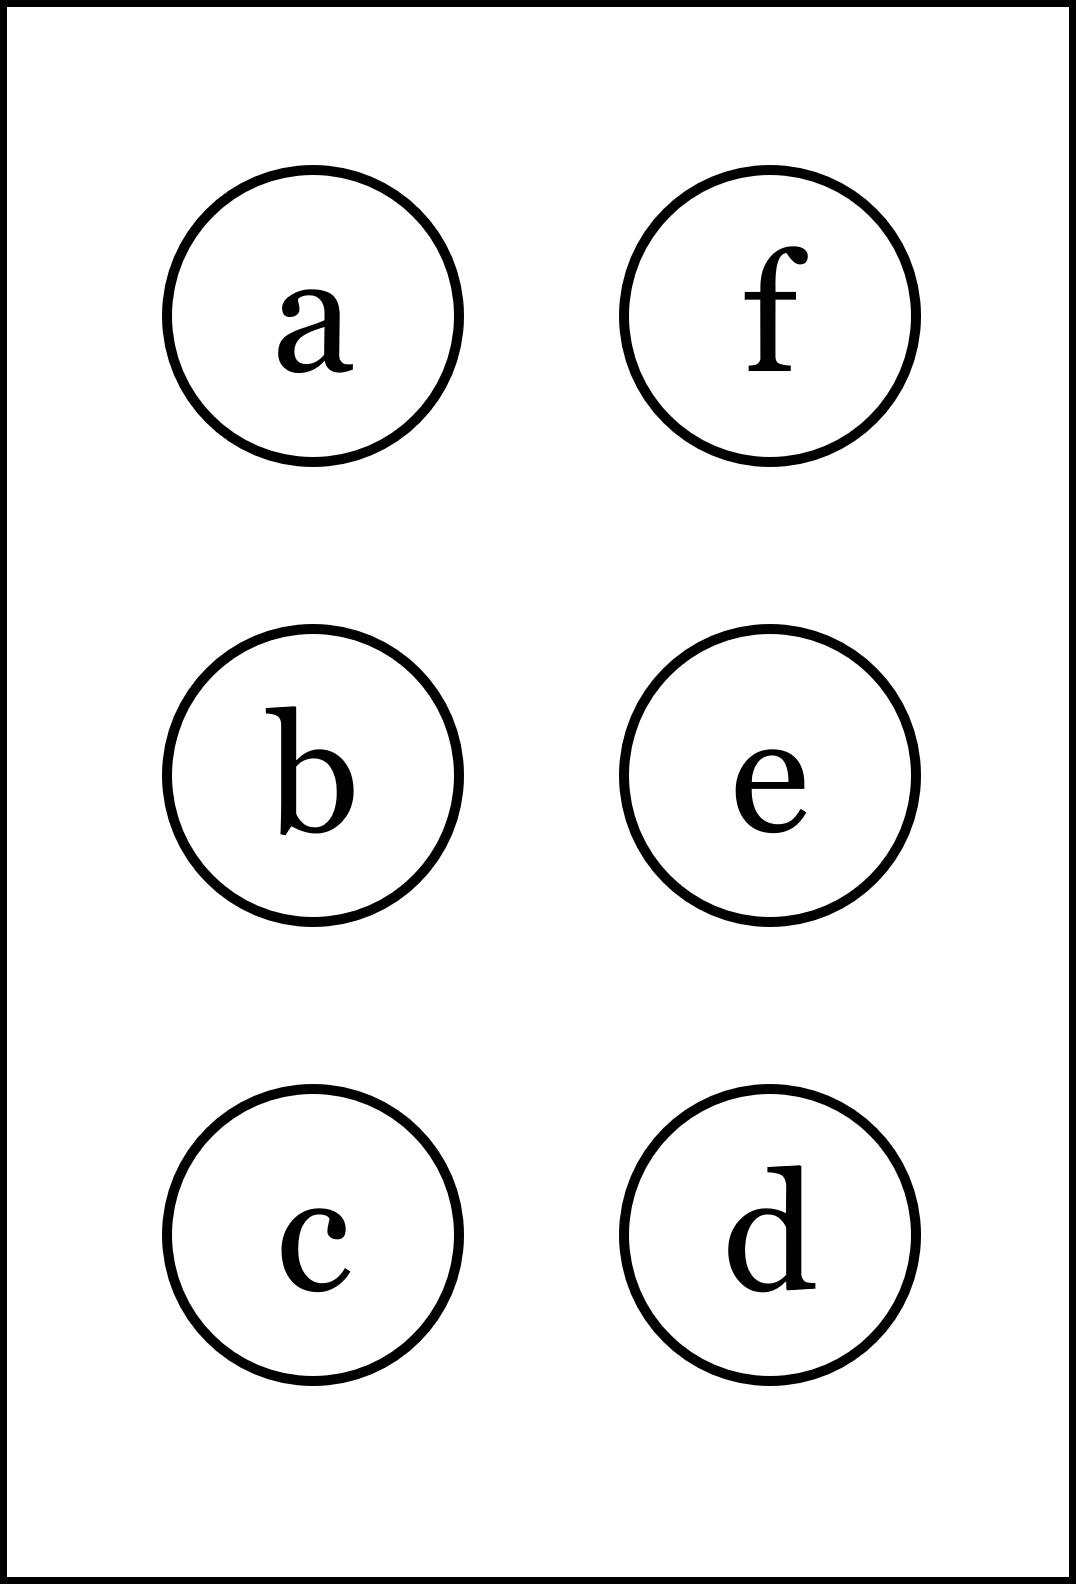
\includegraphics[height=40mm]{../images/braille.png}
{\small Písmeno Braillovej abecedy}
\end{center}
\end{minipage}
\end{center}
\end{minipage}
&
\begin{minipage}[c][104.5mm][t]{0.5\linewidth}
\begin{center}
\vspace{7mm}
{\huge Odmocniny a limity, skupina \textit{Eta $\eta$} -\romannumeral4}\\[5mm]
\textit{Jméno:}\phantom{xxxxxxxxxxxxxxxxxxxxxxxxxxxxxxxxxxxxxxxxxxxxxxxxxxxxxxxxxxxxxxxxx}\\[5mm]
\begin{minipage}{0.95\linewidth}
\begin{center}
V \textbf{(a)} a \textbf{(b)} \textbf{uprav výrazy}, v \textbf{(c)} a \textbf{(d)} \textbf{vypočítaj limity}.\\Pokud se výsledky shodujú s tými za otazníky, tak napravo obarvi\\příslušející kroužek načerno. \textbf{Spolu odevzdejte výsledné slovo}.
\end{center}
\end{minipage}
\\[1mm]
\begin{minipage}{0.79\linewidth}
\begin{center}
\begin{varwidth}{\linewidth}
\begin{enumerate}
\small
\item $\sqrt[5]{\left(\cfrac{x^{2}\;x^{1}}{x^{\nicefrac{1}{2}}}\right)^{3}}$\quad \dotfill\; ???\;\dotfill \quad $x^{\nicefrac{3}{2}}$
\item {\footnotesize{\scriptsize$\big(\sqrt{2x+4y}+\sqrt{2x-4y}\big)^2-\big(\sqrt{2x+4y}-\sqrt{2x-4y}\big)^2$}\quad \dotfill\; ???\;\dotfill \quad $8\sqrt{x^2-2y^2}$}
\item $\lim\limits_{n\to\infty}\cfrac{n^{-1/2}}{\sqrt{4n+7}-\sqrt{4n+3}}$\quad \dotfill\; ???\;\dotfill \quad $1$
\item $\lim\limits_{n\to\infty}9n\cfrac{\sqrt{49n^2+5n+5}-\sqrt{49n^2+4}}{\sqrt{25n^2+8n-1}}$\quad \dotfill\; ???\;\dotfill \quad $\nicefrac{9}{7}$
\item \quad \dotfill\; ???\;\dotfill \quad vybarvi
\item \quad \dotfill\; ???\;\dotfill \quad nebarvi
\end{enumerate}
\end{varwidth}
\end{center}
\end{minipage}
\begin{minipage}{0.20\linewidth}
\begin{center}
{\Huge\bfseries 4.} \\[2mm]
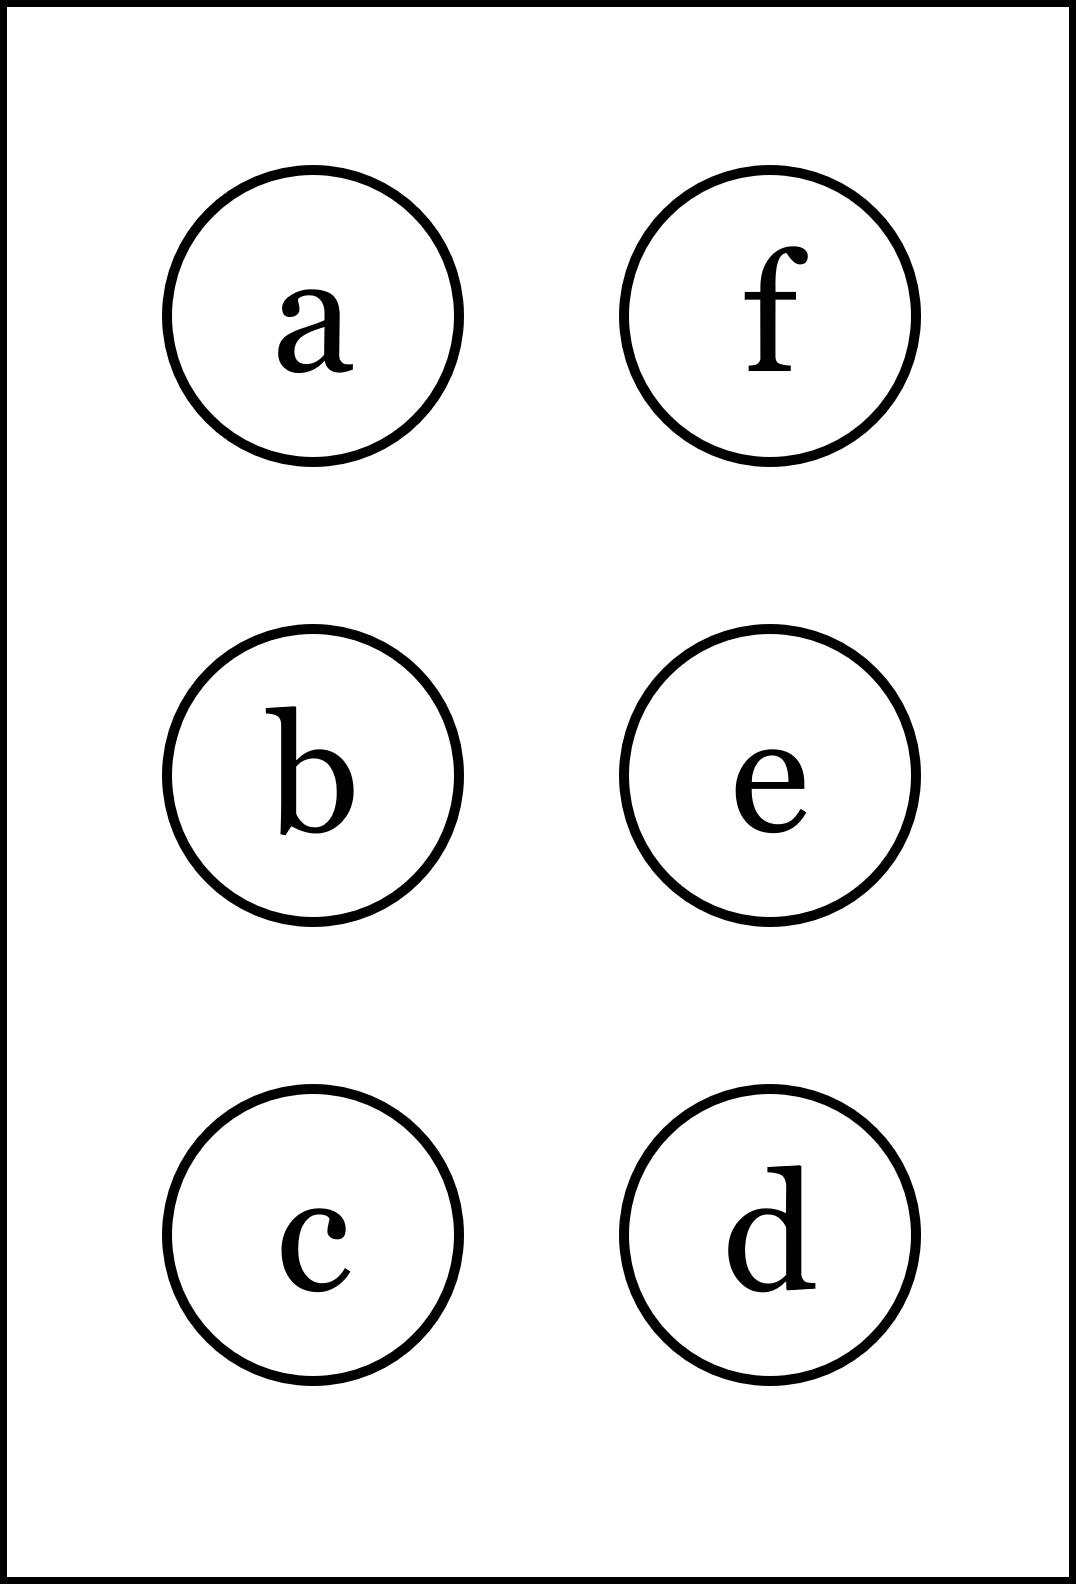
\includegraphics[height=40mm]{../images/braille.png}
{\small Písmeno Braillovej abecedy}
\end{center}
\end{minipage}
\end{center}
\end{minipage}
%
\end{tabular}
\newpage
\thispagestyle{empty}
\begin{tabular}{c:c}
\begin{minipage}[c][104.5mm][t]{0.5\linewidth}
\begin{center}
\vspace{7mm}
{\huge Odmocniny a limity, skupina \textit{Theta $\theta$} -\romannumeral1}\\[5mm]
\textit{Jméno:}\phantom{xxxxxxxxxxxxxxxxxxxxxxxxxxxxxxxxxxxxxxxxxxxxxxxxxxxxxxxxxxxxxxxxx}\\[5mm]
\begin{minipage}{0.95\linewidth}
\begin{center}
V \textbf{(a)} a \textbf{(b)} \textbf{uprav výrazy}, v \textbf{(c)} a \textbf{(d)} \textbf{vypočítaj limity}.\\Pokud se výsledky shodujú s tými za otazníky, tak napravo obarvi\\příslušející kroužek načerno. \textbf{Spolu odevzdejte výsledné slovo}.
\end{center}
\end{minipage}
\\[1mm]
\begin{minipage}{0.79\linewidth}
\begin{center}
\begin{varwidth}{\linewidth}
\begin{enumerate}
\small
\item $\sqrt[2]{\left(\cfrac{x^{2}\;x^{\nicefrac{-2}{3}}}{x^{-3}}\right)^{2}}$\quad \dotfill\; ???\;\dotfill \quad $x^{\nicefrac{17}{3}}$
\item {\footnotesize{\scriptsize$\big(\sqrt{4x-8y}+\sqrt{4x+8y}\big)^2-\big(\sqrt{4x-8y}-\sqrt{4x+8y}\big)^2$}\quad \dotfill\; ???\;\dotfill \quad $16\sqrt{x^2-4y^2}$}
\item $\lim\limits_{n\to\infty}\cfrac{n^{-1/2}}{\sqrt{9n-6}-\sqrt{9n+7}}$\quad \dotfill\; ???\;\dotfill \quad $\infty$
\item $\lim\limits_{n\to\infty}4n\cfrac{\sqrt{16n^2-2n-4}-\sqrt{16n^2-3}}{\sqrt{9n^2+6n+1}}$\quad \dotfill\; ???\;\dotfill \quad $\nicefrac{-2}{3}$
\item \quad \dotfill\; ???\;\dotfill \quad vybarvi
\item \quad \dotfill\; ???\;\dotfill \quad vybarvi
\end{enumerate}
\end{varwidth}
\end{center}
\end{minipage}
\begin{minipage}{0.20\linewidth}
\begin{center}
{\Huge\bfseries 1.} \\[2mm]
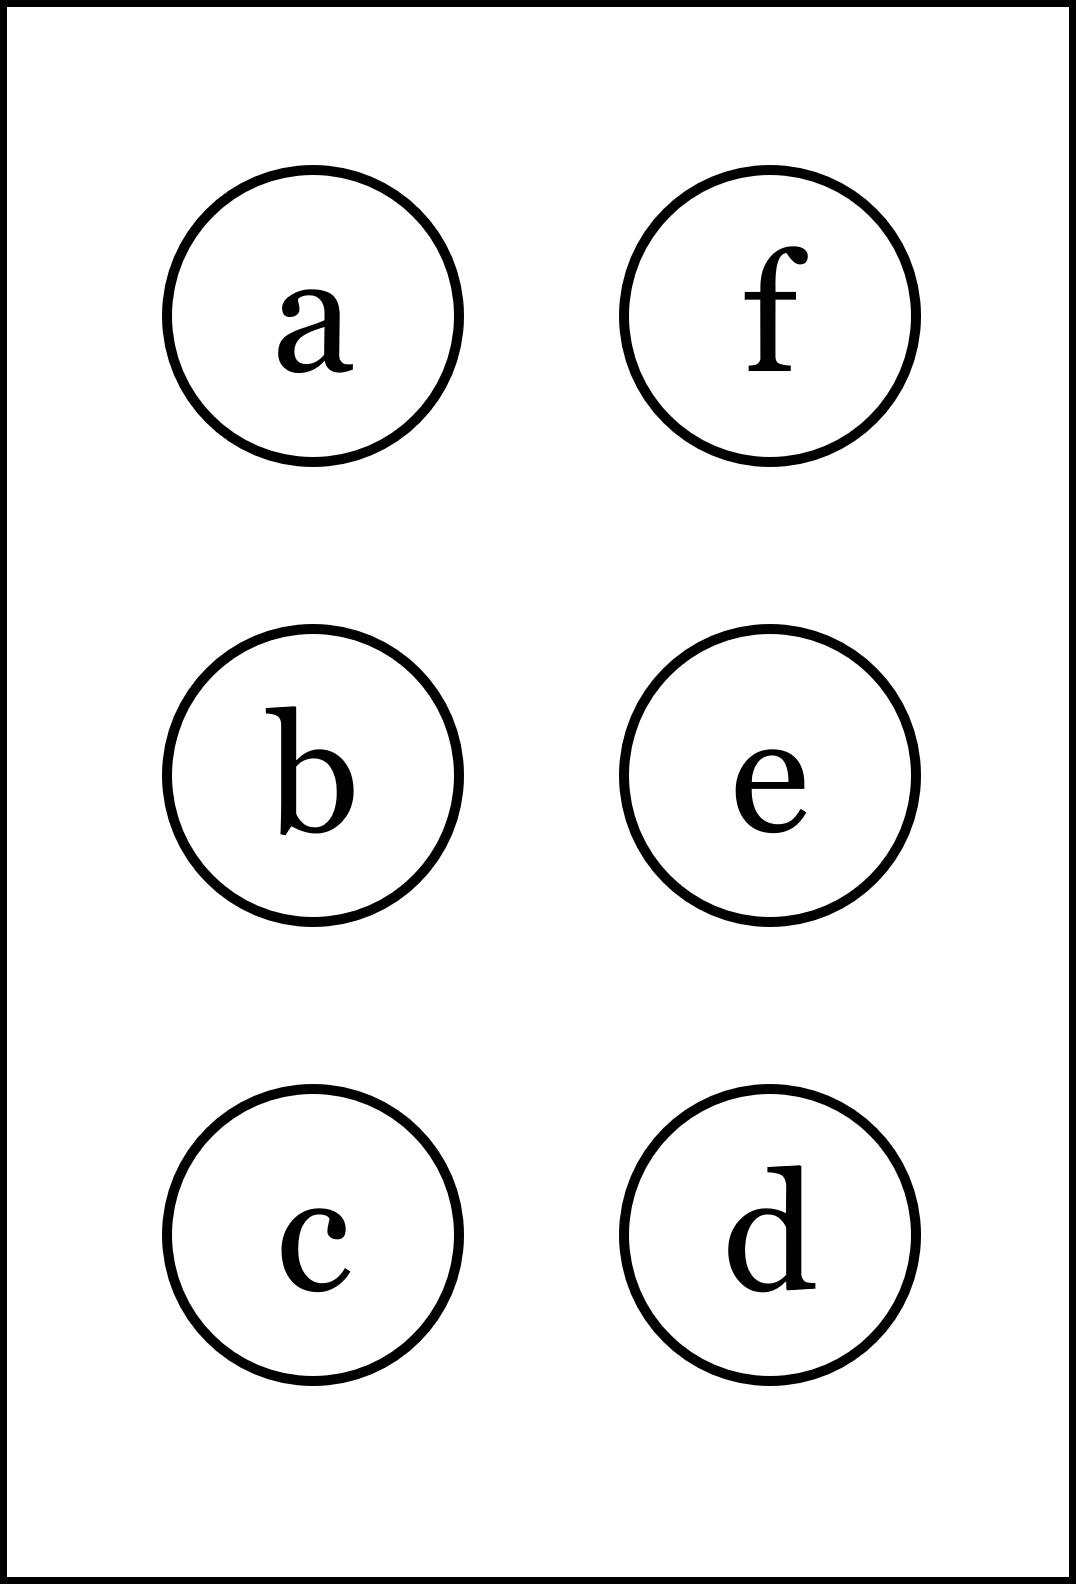
\includegraphics[height=40mm]{../images/braille.png}
{\small Písmeno Braillovej abecedy}
\end{center}
\end{minipage}
\end{center}
\end{minipage}
&
\begin{minipage}[c][104.5mm][t]{0.5\linewidth}
\begin{center}
\vspace{7mm}
{\huge Odmocniny a limity, skupina \textit{Theta $\theta$} -\romannumeral2}\\[5mm]
\textit{Jméno:}\phantom{xxxxxxxxxxxxxxxxxxxxxxxxxxxxxxxxxxxxxxxxxxxxxxxxxxxxxxxxxxxxxxxxx}\\[5mm]
\begin{minipage}{0.95\linewidth}
\begin{center}
V \textbf{(a)} a \textbf{(b)} \textbf{uprav výrazy}, v \textbf{(c)} a \textbf{(d)} \textbf{vypočítaj limity}.\\Pokud se výsledky shodujú s tými za otazníky, tak napravo obarvi\\příslušející kroužek načerno. \textbf{Spolu odevzdejte výsledné slovo}.
\end{center}
\end{minipage}
\\[1mm]
\begin{minipage}{0.79\linewidth}
\begin{center}
\begin{varwidth}{\linewidth}
\begin{enumerate}
\small
\item $\sqrt[1]{\left(\cfrac{x^{\nicefrac{1}{4}}\;x^{\nicefrac{-7}{2}}}{x^{-4}}\right)^{3}}$\quad \dotfill\; ???\;\dotfill \quad $x^{\nicefrac{9}{4}}$
\item {\footnotesize{\scriptsize$\big(\sqrt{4x+24y}+\sqrt{4x-24y}\big)^2-\big(\sqrt{4x+24y}-\sqrt{4x-24y}\big)^2$}\quad \dotfill\; ???\;\dotfill \quad $16\sqrt{x^2-6y^2}$}
\item $\lim\limits_{n\to\infty}\cfrac{n^{-1/2}}{\sqrt{9n+6}-\sqrt{9n+3}}$\quad \dotfill\; ???\;\dotfill \quad $-\infty$
\item $\lim\limits_{n\to\infty}2n\cfrac{\sqrt{n^2+9n+2}-\sqrt{n^2-1}}{\sqrt{16n^2+5n+4}}$\quad \dotfill\; ???\;\dotfill \quad $\nicefrac{9}{2}$
\item \quad \dotfill\; ???\;\dotfill \quad nebarvi
\item \quad \dotfill\; ???\;\dotfill \quad nebarvi
\end{enumerate}
\end{varwidth}
\end{center}
\end{minipage}
\begin{minipage}{0.20\linewidth}
\begin{center}
{\Huge\bfseries 2.} \\[2mm]
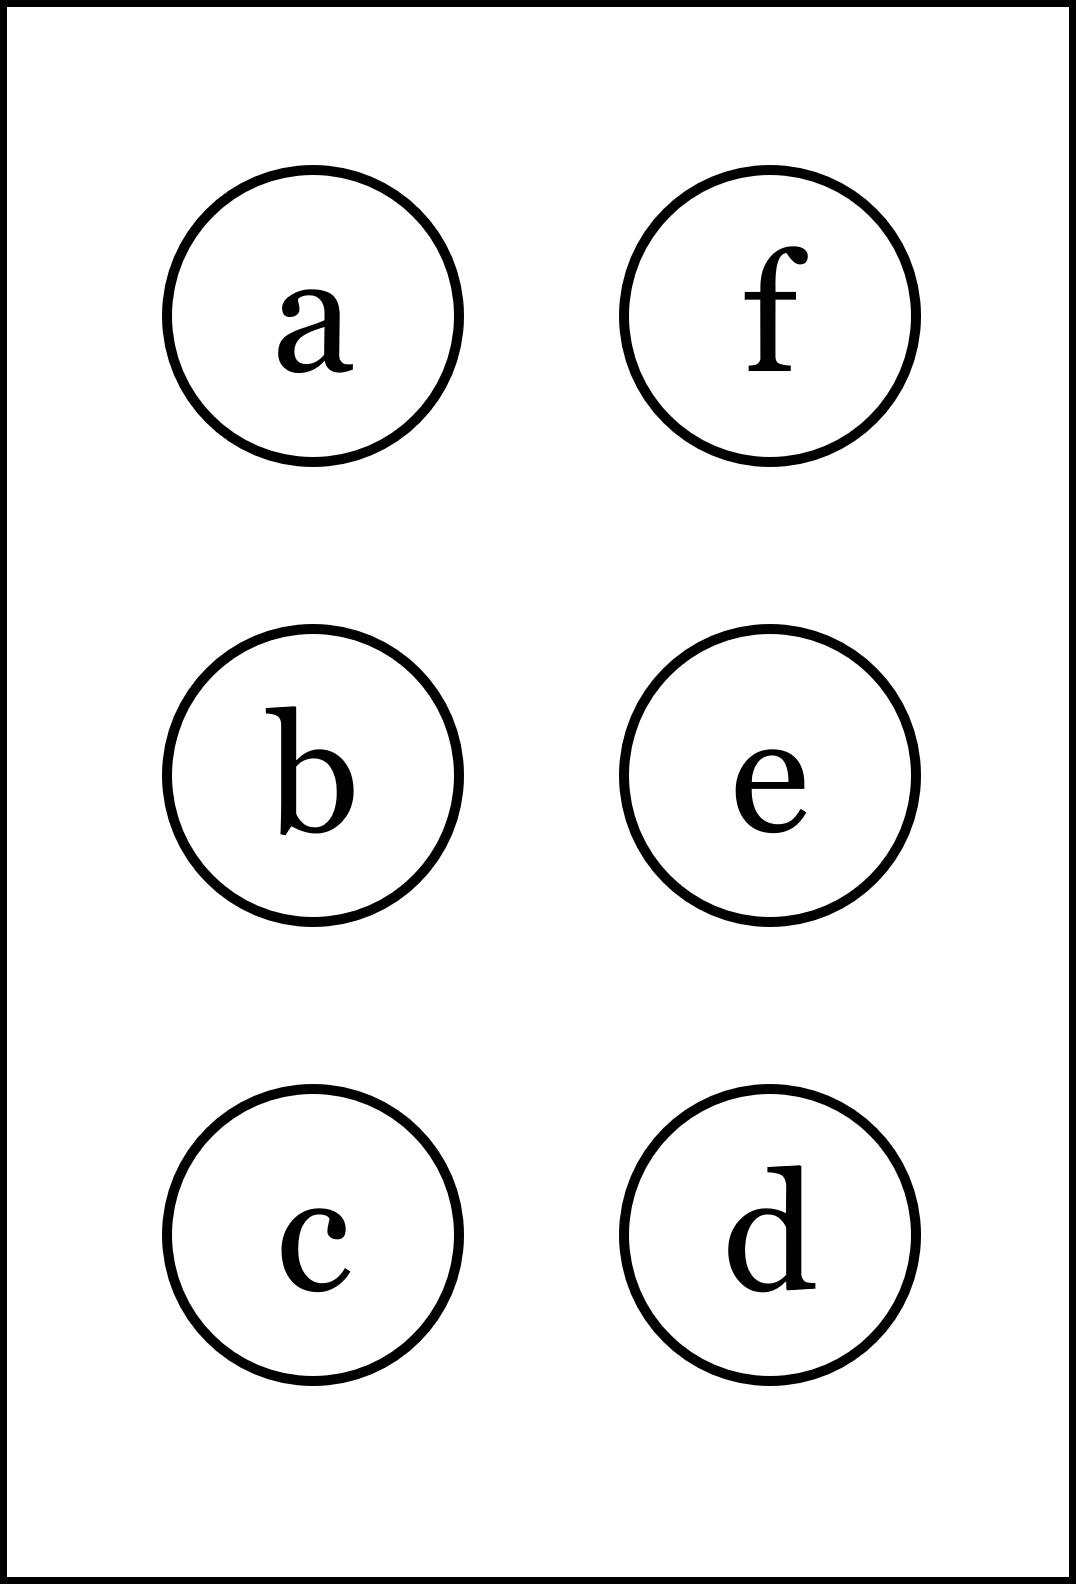
\includegraphics[height=40mm]{../images/braille.png}
{\small Písmeno Braillovej abecedy}
\end{center}
\end{minipage}
\end{center}
\end{minipage}
\\ \hdashline
\begin{minipage}[c][104.5mm][t]{0.5\linewidth}
\begin{center}
\vspace{7mm}
{\huge Odmocniny a limity, skupina \textit{Theta $\theta$} -\romannumeral3}\\[5mm]
\textit{Jméno:}\phantom{xxxxxxxxxxxxxxxxxxxxxxxxxxxxxxxxxxxxxxxxxxxxxxxxxxxxxxxxxxxxxxxxx}\\[5mm]
\begin{minipage}{0.95\linewidth}
\begin{center}
V \textbf{(a)} a \textbf{(b)} \textbf{uprav výrazy}, v \textbf{(c)} a \textbf{(d)} \textbf{vypočítaj limity}.\\Pokud se výsledky shodujú s tými za otazníky, tak napravo obarvi\\příslušející kroužek načerno. \textbf{Spolu odevzdejte výsledné slovo}.
\end{center}
\end{minipage}
\\[1mm]
\begin{minipage}{0.79\linewidth}
\begin{center}
\begin{varwidth}{\linewidth}
\begin{enumerate}
\small
\item $\sqrt[3]{\left(\cfrac{x^{1}\;x^{\nicefrac{2}{5}}}{x^{\nicefrac{-2}{3}}}\right)^{3}}$\quad \dotfill\; ???\;\dotfill \quad $x^{\nicefrac{31}{15}}$
\item {\footnotesize{\scriptsize$\big(\sqrt{4x+16y}+\sqrt{4x-16y}\big)^2-\big(\sqrt{4x+16y}-\sqrt{4x-16y}\big)^2$}\quad \dotfill\; ???\;\dotfill \quad $16\sqrt{x^2-4y^2}$}
\item $\lim\limits_{n\to\infty}\cfrac{n^{-1/2}}{\sqrt{81n-2}-\sqrt{81n-4}}$\quad \dotfill\; ???\;\dotfill \quad $9$
\item $\lim\limits_{n\to\infty}6n\cfrac{\sqrt{49n^2+5n-3}-\sqrt{49n^2+1}}{\sqrt{36n^2-7n+2}}$\quad \dotfill\; ???\;\dotfill \quad $\nicefrac{5}{7}$
\item \quad \dotfill\; ???\;\dotfill \quad nebarvi
\item \quad \dotfill\; ???\;\dotfill \quad nebarvi
\end{enumerate}
\end{varwidth}
\end{center}
\end{minipage}
\begin{minipage}{0.20\linewidth}
\begin{center}
{\Huge\bfseries 3.} \\[2mm]
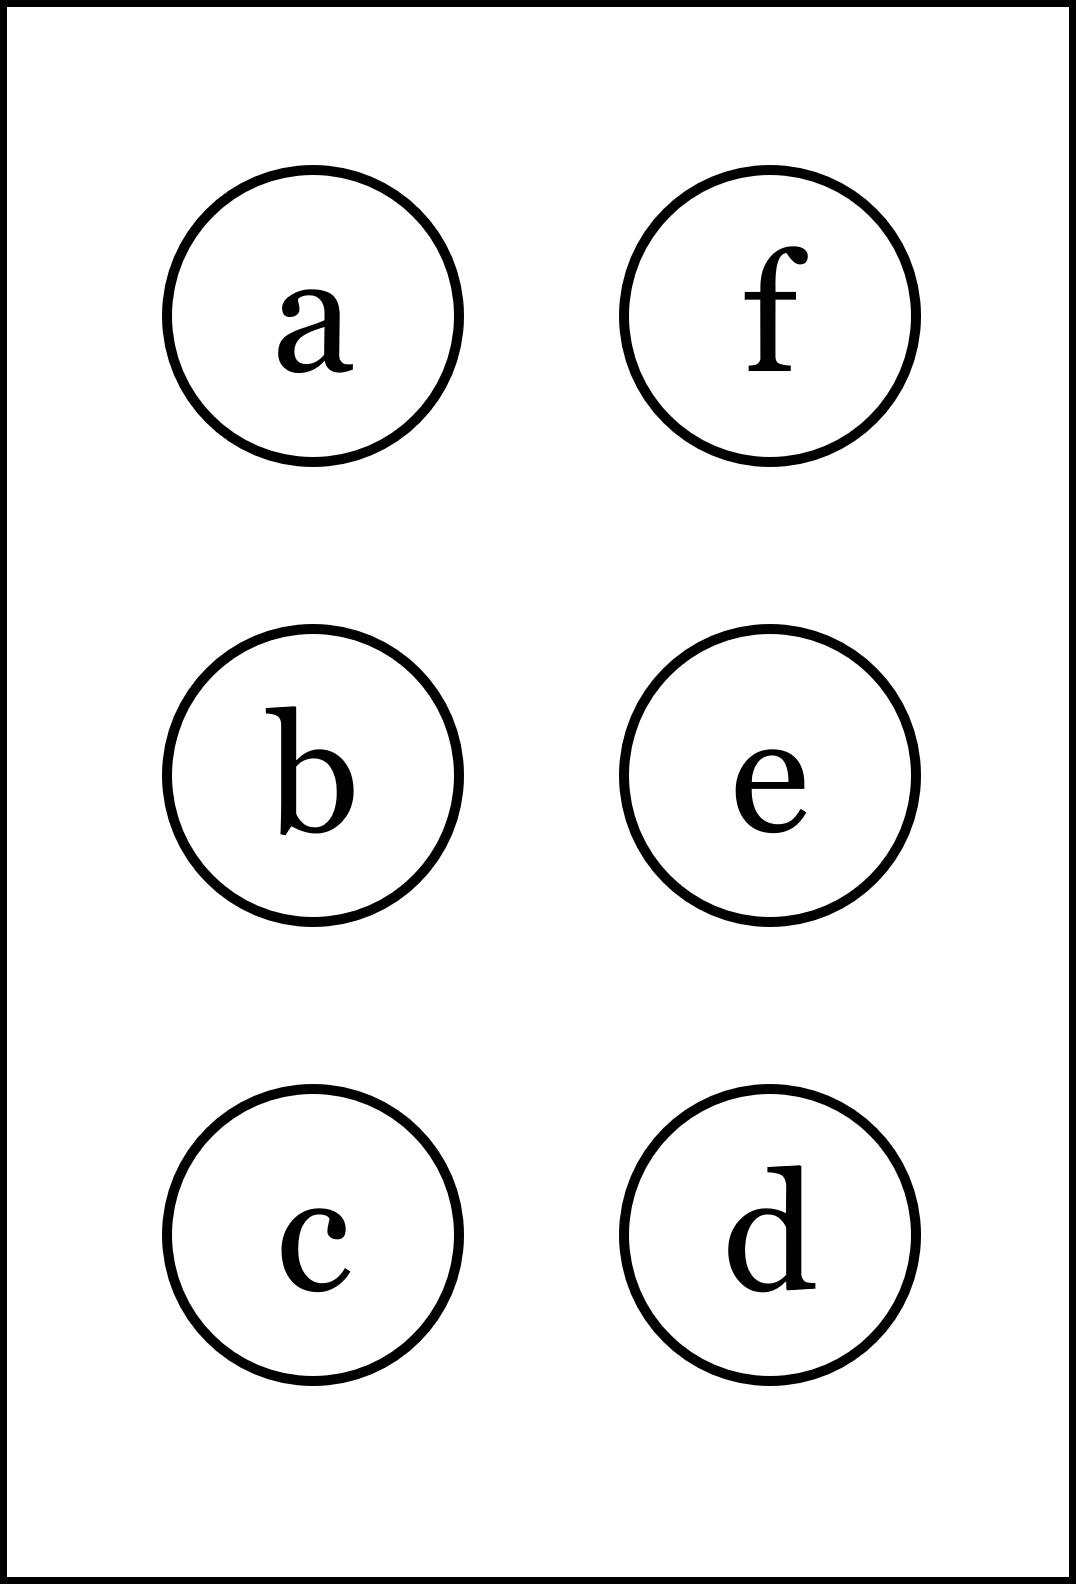
\includegraphics[height=40mm]{../images/braille.png}
{\small Písmeno Braillovej abecedy}
\end{center}
\end{minipage}
\end{center}
\end{minipage}
&
\begin{minipage}[c][104.5mm][t]{0.5\linewidth}
\begin{center}
\vspace{7mm}
{\huge Odmocniny a limity, skupina \textit{Theta $\theta$} -\romannumeral4}\\[5mm]
\textit{Jméno:}\phantom{xxxxxxxxxxxxxxxxxxxxxxxxxxxxxxxxxxxxxxxxxxxxxxxxxxxxxxxxxxxxxxxxx}\\[5mm]
\begin{minipage}{0.95\linewidth}
\begin{center}
V \textbf{(a)} a \textbf{(b)} \textbf{uprav výrazy}, v \textbf{(c)} a \textbf{(d)} \textbf{vypočítaj limity}.\\Pokud se výsledky shodujú s tými za otazníky, tak napravo obarvi\\příslušející kroužek načerno. \textbf{Spolu odevzdejte výsledné slovo}.
\end{center}
\end{minipage}
\\[1mm]
\begin{minipage}{0.79\linewidth}
\begin{center}
\begin{varwidth}{\linewidth}
\begin{enumerate}
\small
\item $\sqrt[7]{\left(\cfrac{x^{1}\;x^{-2}}{x^{\nicefrac{-1}{2}}}\right)^{2}}$\quad \dotfill\; ???\;\dotfill \quad $x^{\nicefrac{-1}{7}}$
\item {\footnotesize{\scriptsize$\big(\sqrt{3x+9y}+\sqrt{3x-9y}\big)^2-\big(\sqrt{3x+9y}-\sqrt{3x-9y}\big)^2$}\quad \dotfill\; ???\;\dotfill \quad $12\sqrt{x^2-3y^2}$}
\item $\lim\limits_{n\to\infty}\cfrac{n^{-1/2}}{\sqrt{36n+8}-\sqrt{36n+1}}$\quad \dotfill\; ???\;\dotfill \quad $\nicefrac{12}{7}$
\item $\lim\limits_{n\to\infty}9n\cfrac{\sqrt{9n^2+5n-6}-\sqrt{9n^2-2}}{\sqrt{49n^2+n+3}}$\quad \dotfill\; ???\;\dotfill \quad $\nicefrac{15}{7}$
\item \quad \dotfill\; ???\;\dotfill \quad vybarvi
\item \quad \dotfill\; ???\;\dotfill \quad nebarvi
\end{enumerate}
\end{varwidth}
\end{center}
\end{minipage}
\begin{minipage}{0.20\linewidth}
\begin{center}
{\Huge\bfseries 4.} \\[2mm]
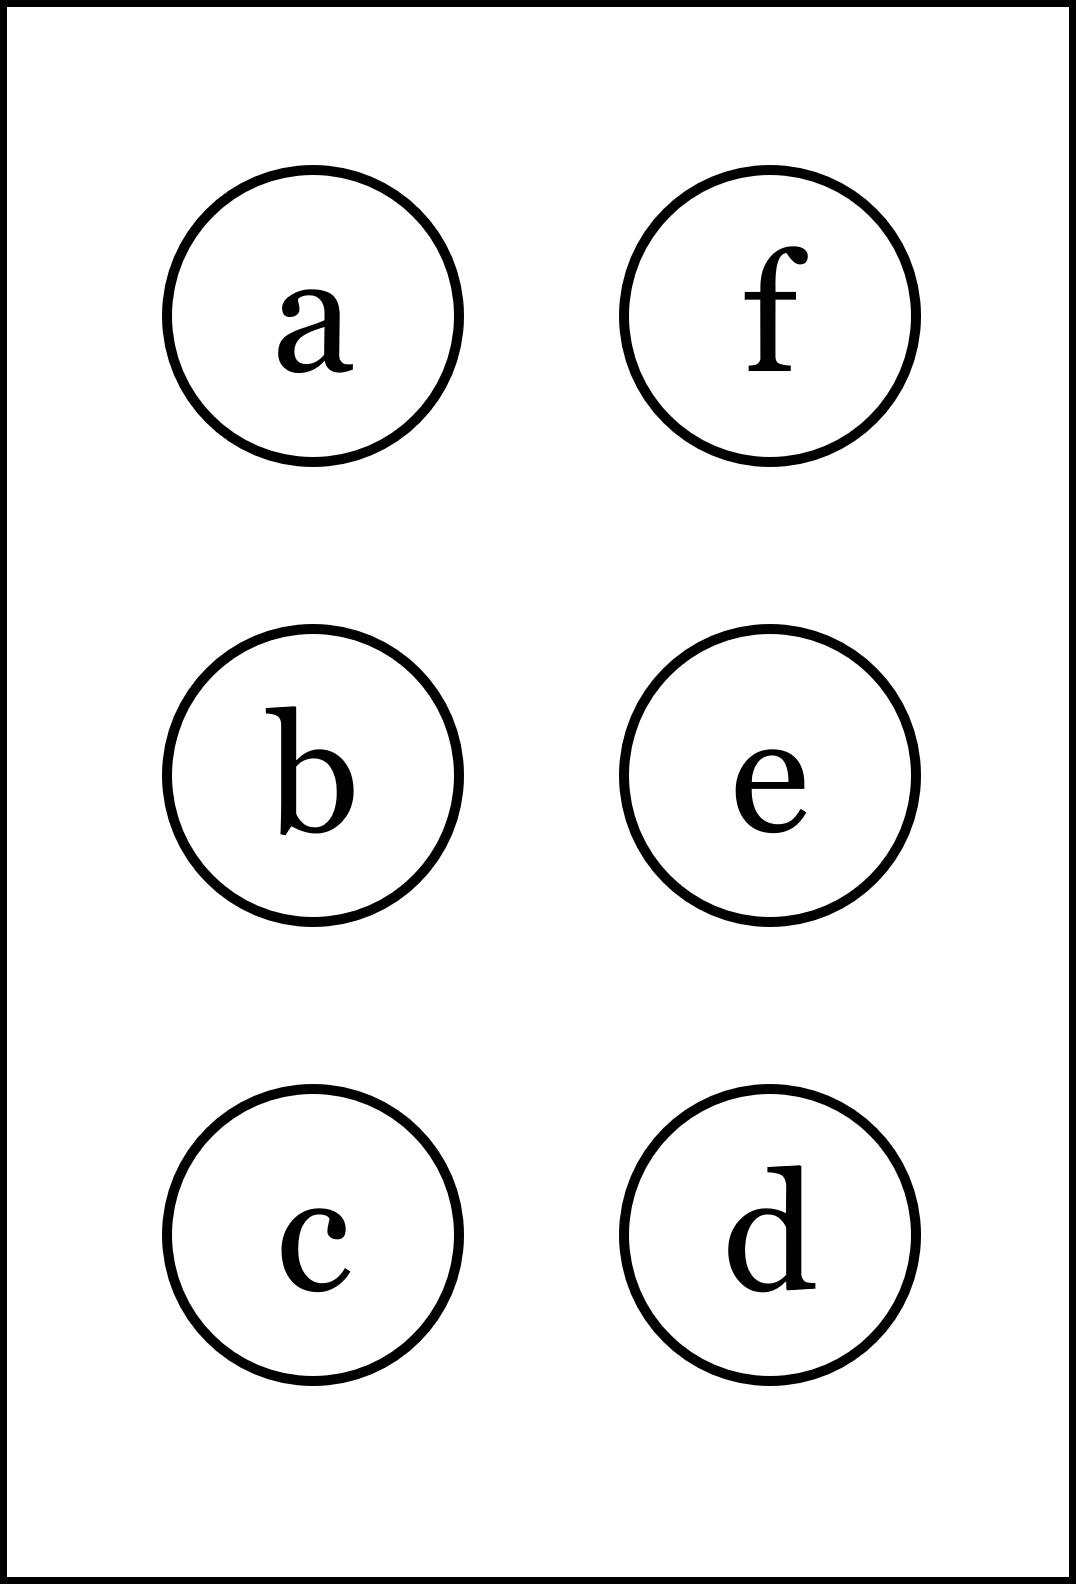
\includegraphics[height=40mm]{../images/braille.png}
{\small Písmeno Braillovej abecedy}
\end{center}
\end{minipage}
\end{center}
\end{minipage}
%
\end{tabular}
\newpage
\thispagestyle{empty}
\begin{tabular}{c:c}
\begin{minipage}[c][104.5mm][t]{0.5\linewidth}
\begin{center}
\vspace{7mm}
{\huge Odmocniny a limity, skupina \textit{Iota $\iota$} -\romannumeral1}\\[5mm]
\textit{Jméno:}\phantom{xxxxxxxxxxxxxxxxxxxxxxxxxxxxxxxxxxxxxxxxxxxxxxxxxxxxxxxxxxxxxxxxx}\\[5mm]
\begin{minipage}{0.95\linewidth}
\begin{center}
V \textbf{(a)} a \textbf{(b)} \textbf{uprav výrazy}, v \textbf{(c)} a \textbf{(d)} \textbf{vypočítaj limity}.\\Pokud se výsledky shodujú s tými za otazníky, tak napravo obarvi\\příslušející kroužek načerno. \textbf{Spolu odevzdejte výsledné slovo}.
\end{center}
\end{minipage}
\\[1mm]
\begin{minipage}{0.79\linewidth}
\begin{center}
\begin{varwidth}{\linewidth}
\begin{enumerate}
\small
\item $\sqrt[2]{\left(\cfrac{x^{-1}\;x^{1}}{x^{\nicefrac{-2}{3}}}\right)^{2}}$\quad \dotfill\; ???\;\dotfill \quad $x^{\nicefrac{2}{3}}$
\item {\footnotesize{\scriptsize$\big(\sqrt{2x-16y}+\sqrt{2x+16y}\big)^2-\big(\sqrt{2x-16y}-\sqrt{2x+16y}\big)^2$}\quad \dotfill\; ???\;\dotfill \quad $8\sqrt{x^2+8y^2}$}
\item $\lim\limits_{n\to\infty}\cfrac{n^{-1/2}}{\sqrt{49n+6}-\sqrt{49n-3}}$\quad \dotfill\; ???\;\dotfill \quad $-\infty$
\item $\lim\limits_{n\to\infty}3n\cfrac{\sqrt{n^2-2n-1}-\sqrt{n^2-3}}{\sqrt{16n^2+8n-1}}$\quad \dotfill\; ???\;\dotfill \quad $\nicefrac{-3}{2}$
\item \quad \dotfill\; ???\;\dotfill \quad nebarvi
\item \quad \dotfill\; ???\;\dotfill \quad vybarvi
\end{enumerate}
\end{varwidth}
\end{center}
\end{minipage}
\begin{minipage}{0.20\linewidth}
\begin{center}
{\Huge\bfseries 1.} \\[2mm]
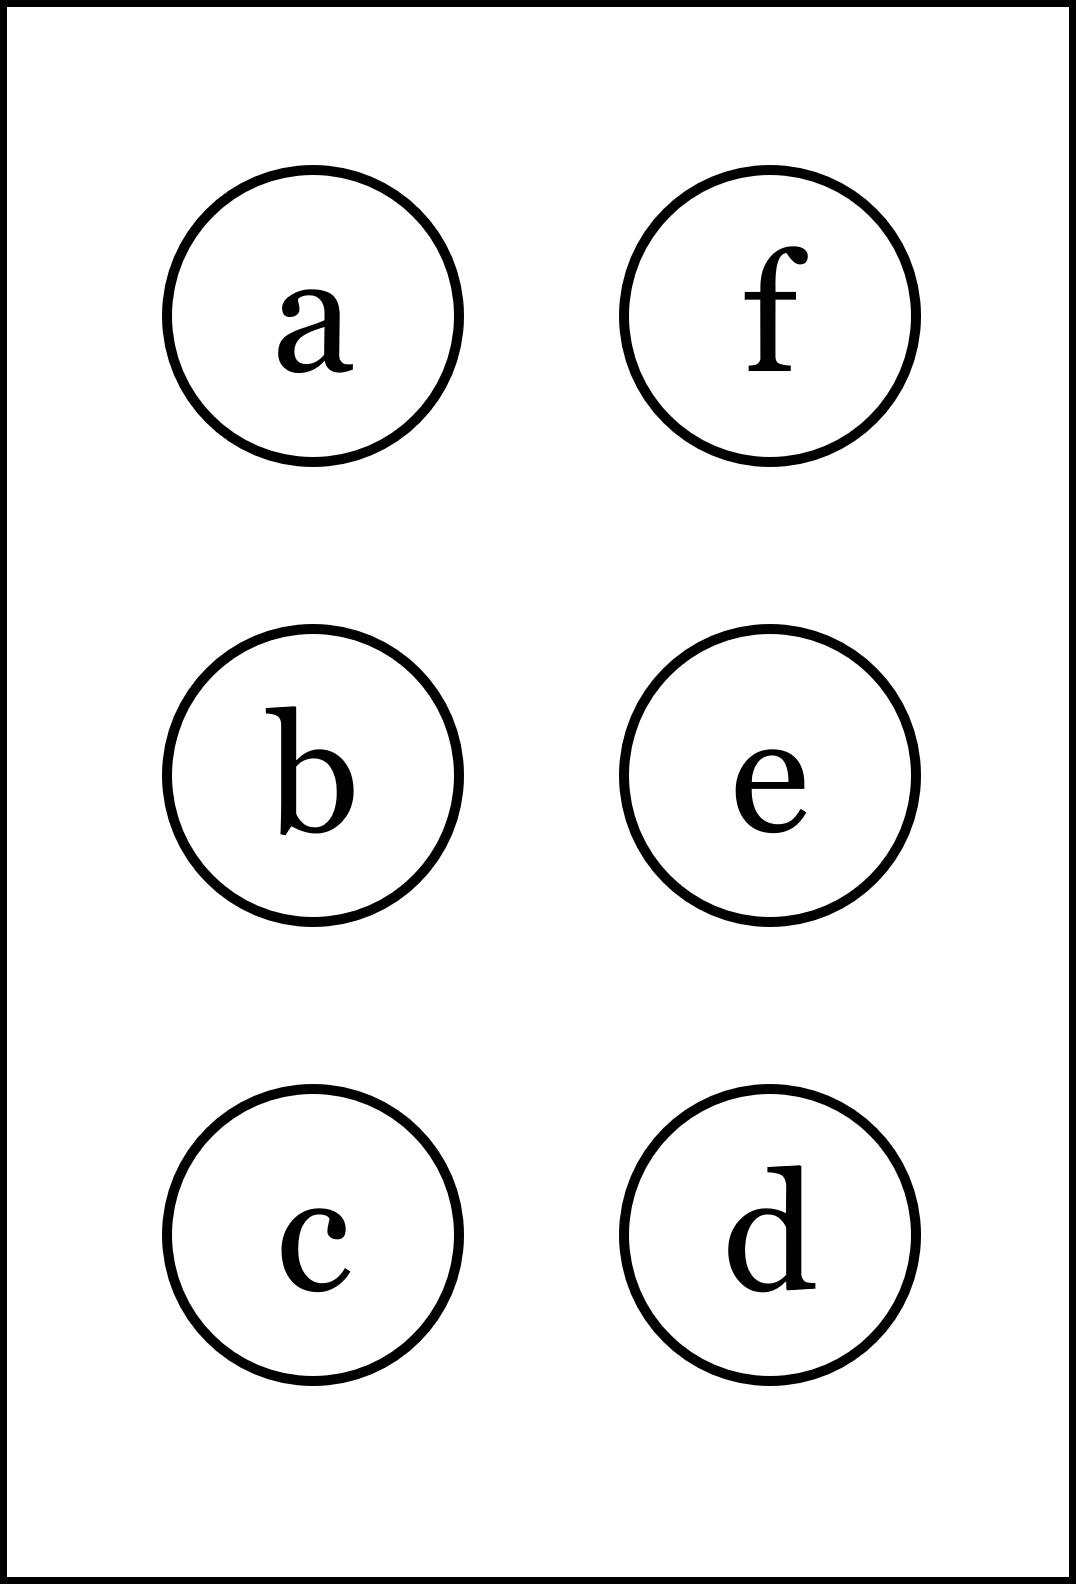
\includegraphics[height=40mm]{../images/braille.png}
{\small Písmeno Braillovej abecedy}
\end{center}
\end{minipage}
\end{center}
\end{minipage}
&
\begin{minipage}[c][104.5mm][t]{0.5\linewidth}
\begin{center}
\vspace{7mm}
{\huge Odmocniny a limity, skupina \textit{Iota $\iota$} -\romannumeral2}\\[5mm]
\textit{Jméno:}\phantom{xxxxxxxxxxxxxxxxxxxxxxxxxxxxxxxxxxxxxxxxxxxxxxxxxxxxxxxxxxxxxxxxx}\\[5mm]
\begin{minipage}{0.95\linewidth}
\begin{center}
V \textbf{(a)} a \textbf{(b)} \textbf{uprav výrazy}, v \textbf{(c)} a \textbf{(d)} \textbf{vypočítaj limity}.\\Pokud se výsledky shodujú s tými za otazníky, tak napravo obarvi\\příslušející kroužek načerno. \textbf{Spolu odevzdejte výsledné slovo}.
\end{center}
\end{minipage}
\\[1mm]
\begin{minipage}{0.79\linewidth}
\begin{center}
\begin{varwidth}{\linewidth}
\begin{enumerate}
\small
\item $\sqrt[3]{\left(\cfrac{x^{\nicefrac{-2}{5}}\;x^{\nicefrac{-3}{2}}}{x^{1}}\right)^{3}}$\quad \dotfill\; ???\;\dotfill \quad $x^{\nicefrac{-29}{10}}$
\item {\footnotesize{\scriptsize$\big(\sqrt{x+3y}+\sqrt{x-3y}\big)^2-\big(\sqrt{x+3y}-\sqrt{x-3y}\big)^2$}\quad \dotfill\; ???\;\dotfill \quad $4\sqrt{x^2-3y^2}$}
\item $\lim\limits_{n\to\infty}\cfrac{n^{-1/2}}{\sqrt{36n-7}-\sqrt{36n+4}}$\quad \dotfill\; ???\;\dotfill \quad $0$
\item $\lim\limits_{n\to\infty}2n\cfrac{\sqrt{25n^2+6n+5}-\sqrt{25n^2+8}}{\sqrt{81n^2-3n-1}}$\quad \dotfill\; ???\;\dotfill \quad $\nicefrac{4}{15}$
\item \quad \dotfill\; ???\;\dotfill \quad vybarvi
\item \quad \dotfill\; ???\;\dotfill \quad nebarvi
\end{enumerate}
\end{varwidth}
\end{center}
\end{minipage}
\begin{minipage}{0.20\linewidth}
\begin{center}
{\Huge\bfseries 2.} \\[2mm]
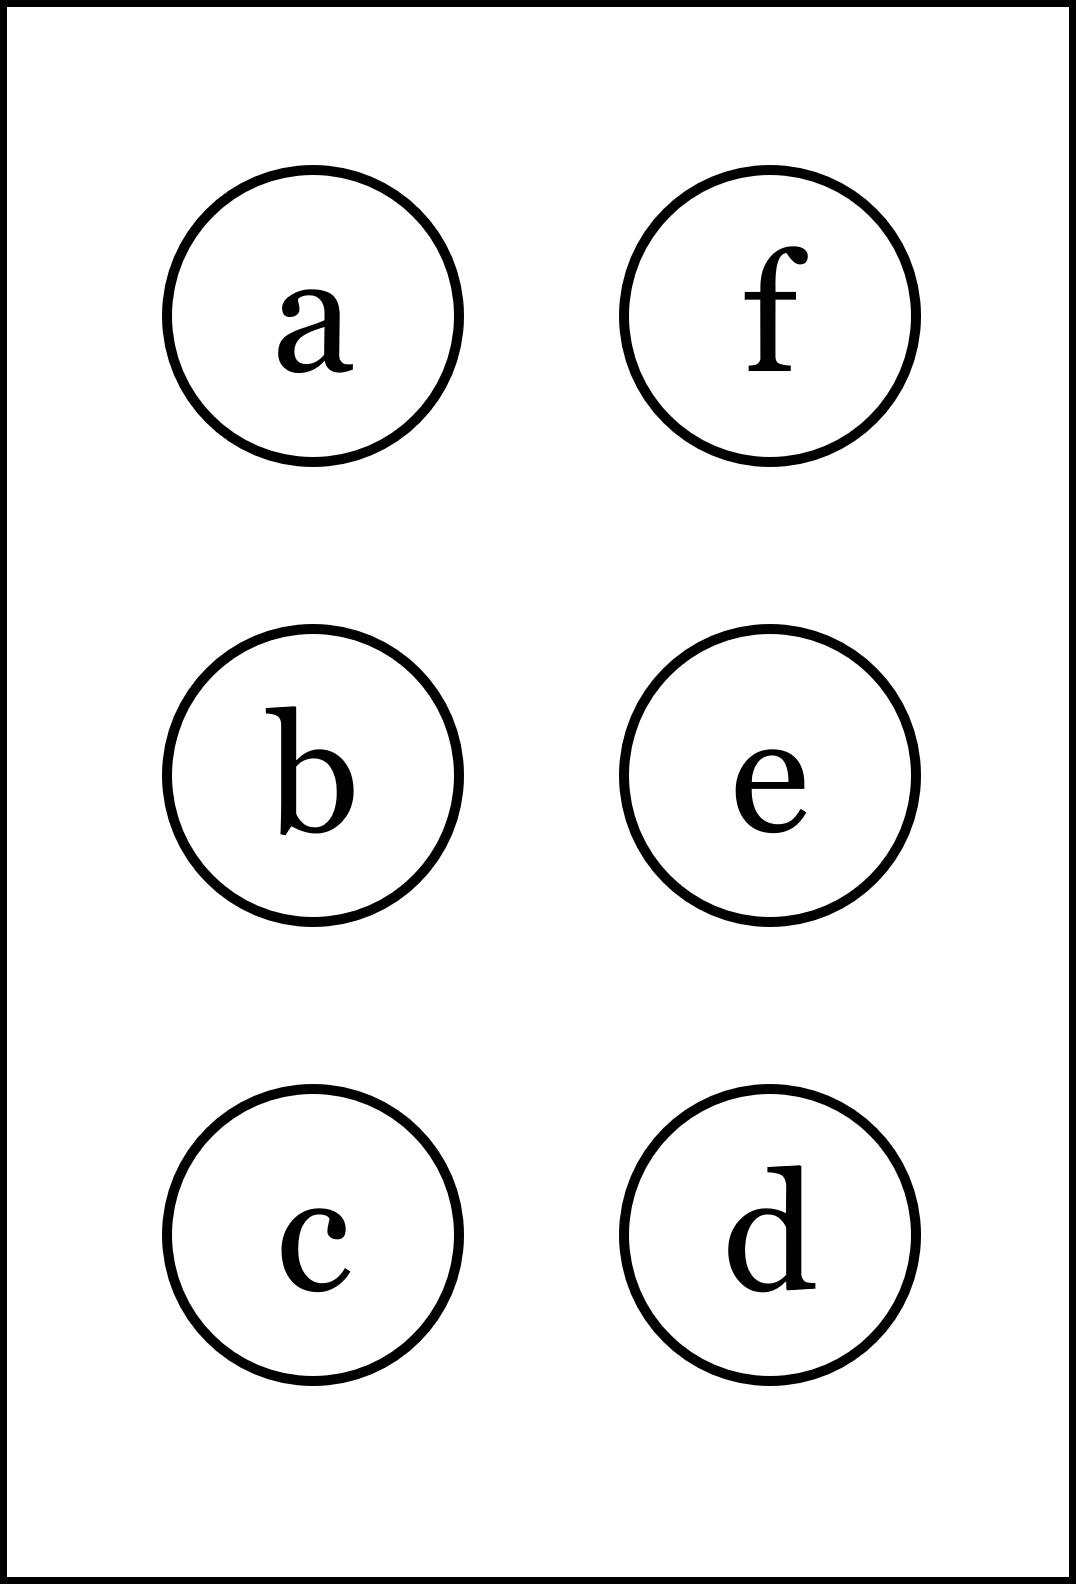
\includegraphics[height=40mm]{../images/braille.png}
{\small Písmeno Braillovej abecedy}
\end{center}
\end{minipage}
\end{center}
\end{minipage}
\\ \hdashline
\begin{minipage}[c][104.5mm][t]{0.5\linewidth}
\begin{center}
\vspace{7mm}
{\huge Odmocniny a limity, skupina \textit{Iota $\iota$} -\romannumeral3}\\[5mm]
\textit{Jméno:}\phantom{xxxxxxxxxxxxxxxxxxxxxxxxxxxxxxxxxxxxxxxxxxxxxxxxxxxxxxxxxxxxxxxxx}\\[5mm]
\begin{minipage}{0.95\linewidth}
\begin{center}
V \textbf{(a)} a \textbf{(b)} \textbf{uprav výrazy}, v \textbf{(c)} a \textbf{(d)} \textbf{vypočítaj limity}.\\Pokud se výsledky shodujú s tými za otazníky, tak napravo obarvi\\příslušející kroužek načerno. \textbf{Spolu odevzdejte výsledné slovo}.
\end{center}
\end{minipage}
\\[1mm]
\begin{minipage}{0.79\linewidth}
\begin{center}
\begin{varwidth}{\linewidth}
\begin{enumerate}
\small
\item $\sqrt[3]{\left(\cfrac{x^{\nicefrac{3}{2}}\;x^{-1}}{x^{\nicefrac{-5}{3}}}\right)^{2}}$\quad \dotfill\; ???\;\dotfill \quad $x^{\nicefrac{13}{9}}$
\item {\footnotesize{\scriptsize$\big(\sqrt{6x-6y}+\sqrt{6x+6y}\big)^2-\big(\sqrt{6x-6y}-\sqrt{6x+6y}\big)^2$}\quad \dotfill\; ???\;\dotfill \quad $24\sqrt{x^2-y^2}$}
\item $\lim\limits_{n\to\infty}\cfrac{n^{-1/2}}{\sqrt{9n-4}-\sqrt{9n-5}}$\quad \dotfill\; ???\;\dotfill \quad $6$
\item $\lim\limits_{n\to\infty}9n\cfrac{\sqrt{16n^2+7n+2}-\sqrt{16n^2-7}}{\sqrt{n^2-2n-5}}$\quad \dotfill\; ???\;\dotfill \quad $\nicefrac{63}{4}$
\item \quad \dotfill\; ???\;\dotfill \quad nebarvi
\item \quad \dotfill\; ???\;\dotfill \quad nebarvi
\end{enumerate}
\end{varwidth}
\end{center}
\end{minipage}
\begin{minipage}{0.20\linewidth}
\begin{center}
{\Huge\bfseries 3.} \\[2mm]
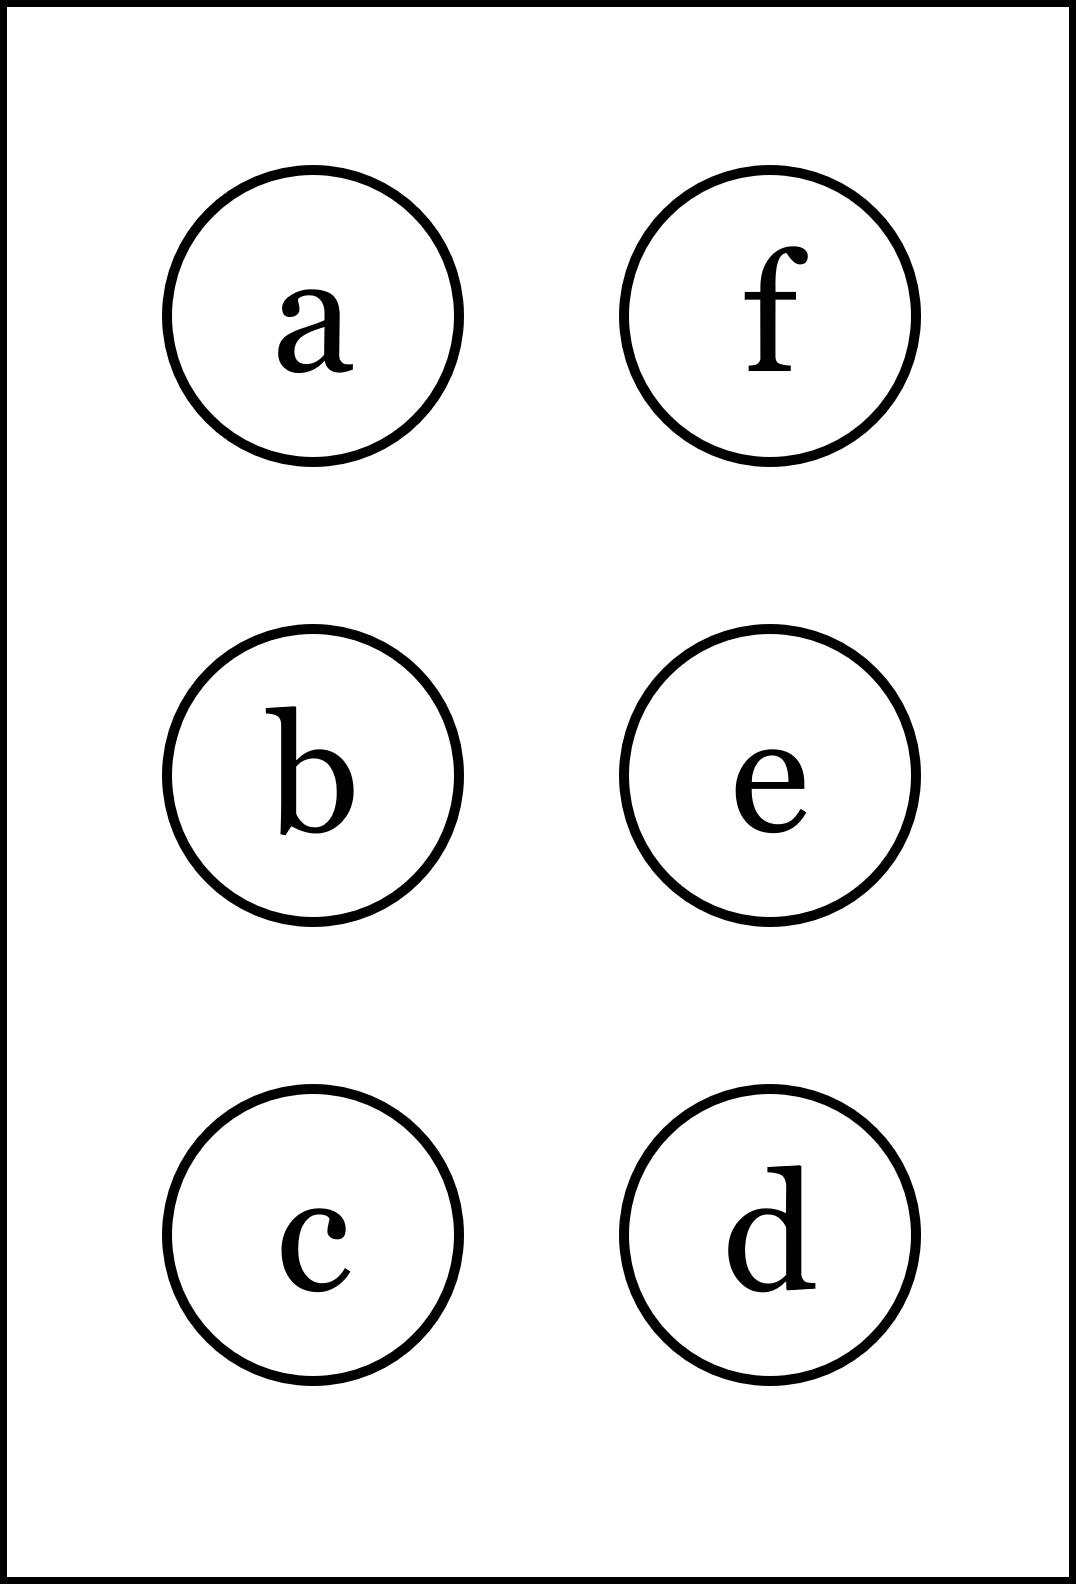
\includegraphics[height=40mm]{../images/braille.png}
{\small Písmeno Braillovej abecedy}
\end{center}
\end{minipage}
\end{center}
\end{minipage}
&
\begin{minipage}[c][104.5mm][t]{0.5\linewidth}
\begin{center}
\vspace{7mm}
{\huge Odmocniny a limity, skupina \textit{Iota $\iota$} -\romannumeral4}\\[5mm]
\textit{Jméno:}\phantom{xxxxxxxxxxxxxxxxxxxxxxxxxxxxxxxxxxxxxxxxxxxxxxxxxxxxxxxxxxxxxxxxx}\\[5mm]
\begin{minipage}{0.95\linewidth}
\begin{center}
V \textbf{(a)} a \textbf{(b)} \textbf{uprav výrazy}, v \textbf{(c)} a \textbf{(d)} \textbf{vypočítaj limity}.\\Pokud se výsledky shodujú s tými za otazníky, tak napravo obarvi\\příslušející kroužek načerno. \textbf{Spolu odevzdejte výsledné slovo}.
\end{center}
\end{minipage}
\\[1mm]
\begin{minipage}{0.79\linewidth}
\begin{center}
\begin{varwidth}{\linewidth}
\begin{enumerate}
\small
\item $\sqrt[2]{\left(\cfrac{x^{1}\;x^{\nicefrac{1}{2}}}{x^{1}}\right)^{2}}$\quad \dotfill\; ???\;\dotfill \quad $x^{\nicefrac{1}{2}}$
\item {\footnotesize{\scriptsize$\big(\sqrt{8x-32y}+\sqrt{8x+32y}\big)^2-\big(\sqrt{8x-32y}-\sqrt{8x+32y}\big)^2$}\quad \dotfill\; ???\;\dotfill \quad $32\sqrt{x^2+4y^2}$}
\item $\lim\limits_{n\to\infty}\cfrac{n^{-1/2}}{\sqrt{n-4}-\sqrt{n-3}}$\quad \dotfill\; ???\;\dotfill \quad $0$
\item $\lim\limits_{n\to\infty}7n\cfrac{\sqrt{4n^2+n-8}-\sqrt{4n^2+5}}{\sqrt{n^2+8n-7}}$\quad \dotfill\; ???\;\dotfill \quad $\nicefrac{7}{2}$
\item \quad \dotfill\; ???\;\dotfill \quad nebarvi
\item \quad \dotfill\; ???\;\dotfill \quad nebarvi
\end{enumerate}
\end{varwidth}
\end{center}
\end{minipage}
\begin{minipage}{0.20\linewidth}
\begin{center}
{\Huge\bfseries 4.} \\[2mm]
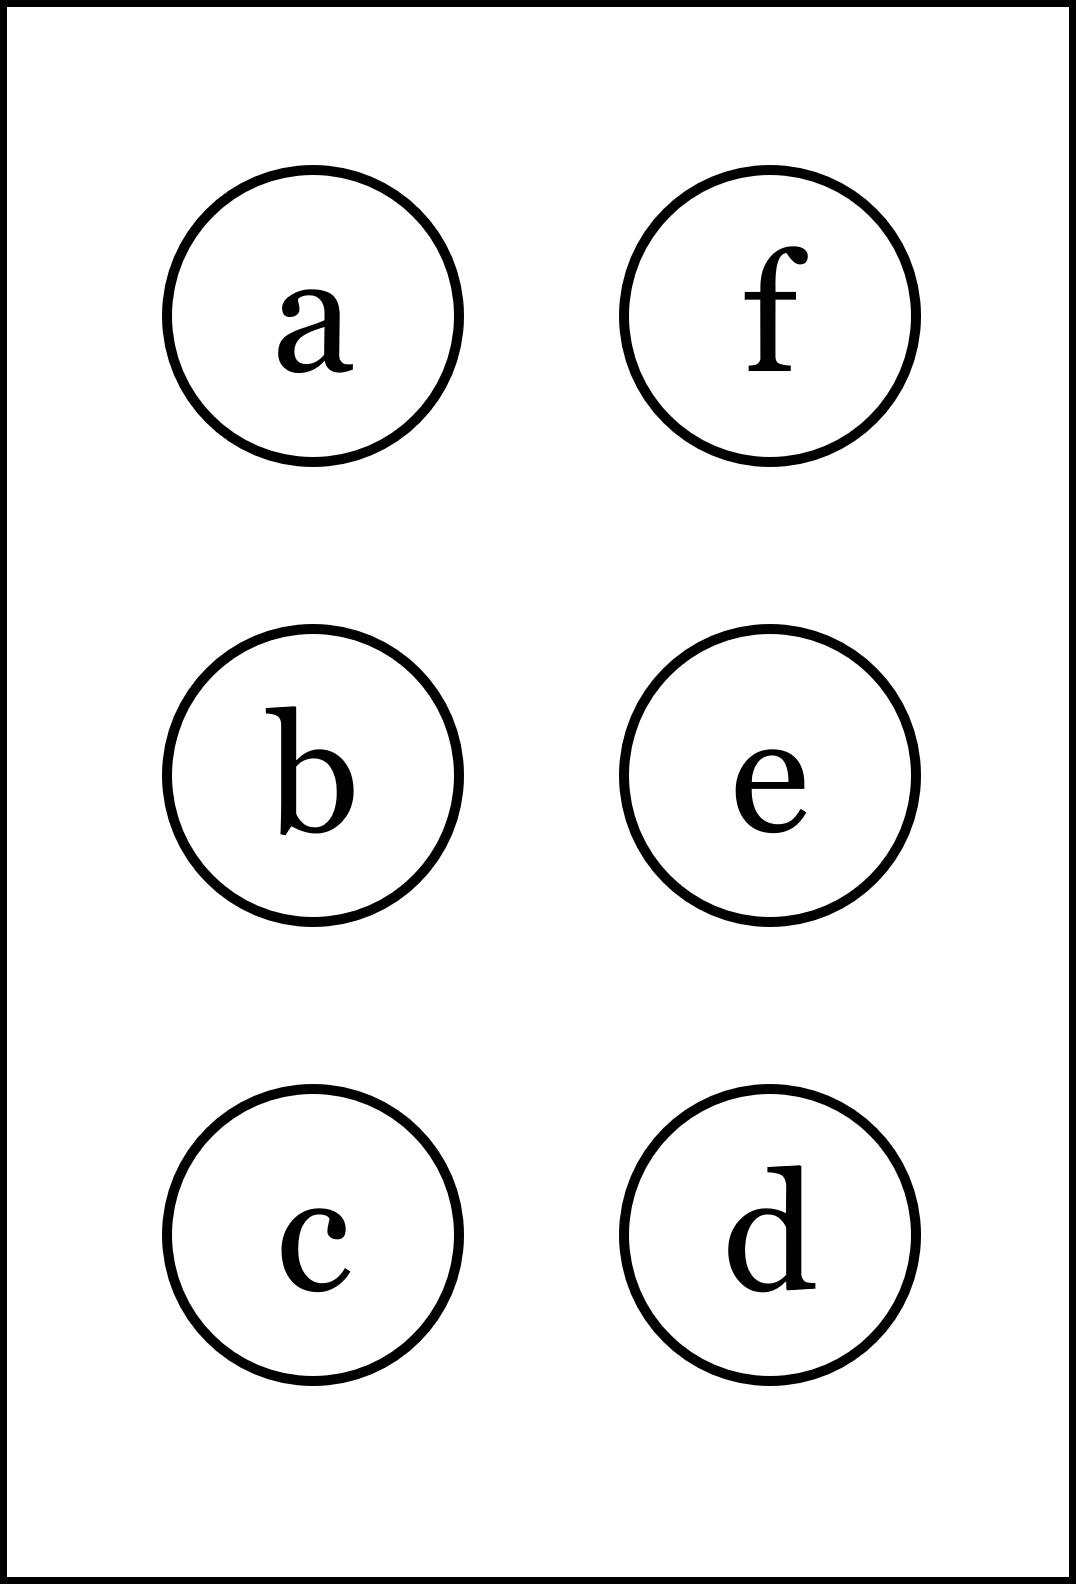
\includegraphics[height=40mm]{../images/braille.png}
{\small Písmeno Braillovej abecedy}
\end{center}
\end{minipage}
\end{center}
\end{minipage}
%
\end{tabular}
\newpage
\thispagestyle{empty}
\begin{tabular}{c:c}
\begin{minipage}[c][104.5mm][t]{0.5\linewidth}
\begin{center}
\vspace{7mm}
{\huge Odmocniny a limity, skupina \textit{Kappa $\kappa$} -\romannumeral1}\\[5mm]
\textit{Jméno:}\phantom{xxxxxxxxxxxxxxxxxxxxxxxxxxxxxxxxxxxxxxxxxxxxxxxxxxxxxxxxxxxxxxxxx}\\[5mm]
\begin{minipage}{0.95\linewidth}
\begin{center}
V \textbf{(a)} a \textbf{(b)} \textbf{uprav výrazy}, v \textbf{(c)} a \textbf{(d)} \textbf{vypočítaj limity}.\\Pokud se výsledky shodujú s tými za otazníky, tak napravo obarvi\\příslušející kroužek načerno. \textbf{Spolu odevzdejte výsledné slovo}.
\end{center}
\end{minipage}
\\[1mm]
\begin{minipage}{0.79\linewidth}
\begin{center}
\begin{varwidth}{\linewidth}
\begin{enumerate}
\small
\item $\sqrt[6]{\left(\cfrac{x^{1}\;x^{-1}}{x^{\nicefrac{-1}{4}}}\right)^{5}}$\quad \dotfill\; ???\;\dotfill \quad $x^{\nicefrac{5}{24}}$
\item {\footnotesize{\scriptsize$\big(\sqrt{2x-6y}+\sqrt{2x+6y}\big)^2-\big(\sqrt{2x-6y}-\sqrt{2x+6y}\big)^2$}\quad \dotfill\; ???\;\dotfill \quad $8\sqrt{x^2+3y^2}$}
\item $\lim\limits_{n\to\infty}\cfrac{n^{-1/2}}{\sqrt{4n-3}-\sqrt{4n+7}}$\quad \dotfill\; ???\;\dotfill \quad $\nicefrac{-2}{5}$
\item $\lim\limits_{n\to\infty}2n\cfrac{\sqrt{81n^2+8n+5}-\sqrt{81n^2+4}}{\sqrt{36n^2+2n+4}}$\quad \dotfill\; ???\;\dotfill \quad $\nicefrac{4}{27}$
\item \quad \dotfill\; ???\;\dotfill \quad vybarvi
\item \quad \dotfill\; ???\;\dotfill \quad nebarvi
\end{enumerate}
\end{varwidth}
\end{center}
\end{minipage}
\begin{minipage}{0.20\linewidth}
\begin{center}
{\Huge\bfseries 1.} \\[2mm]
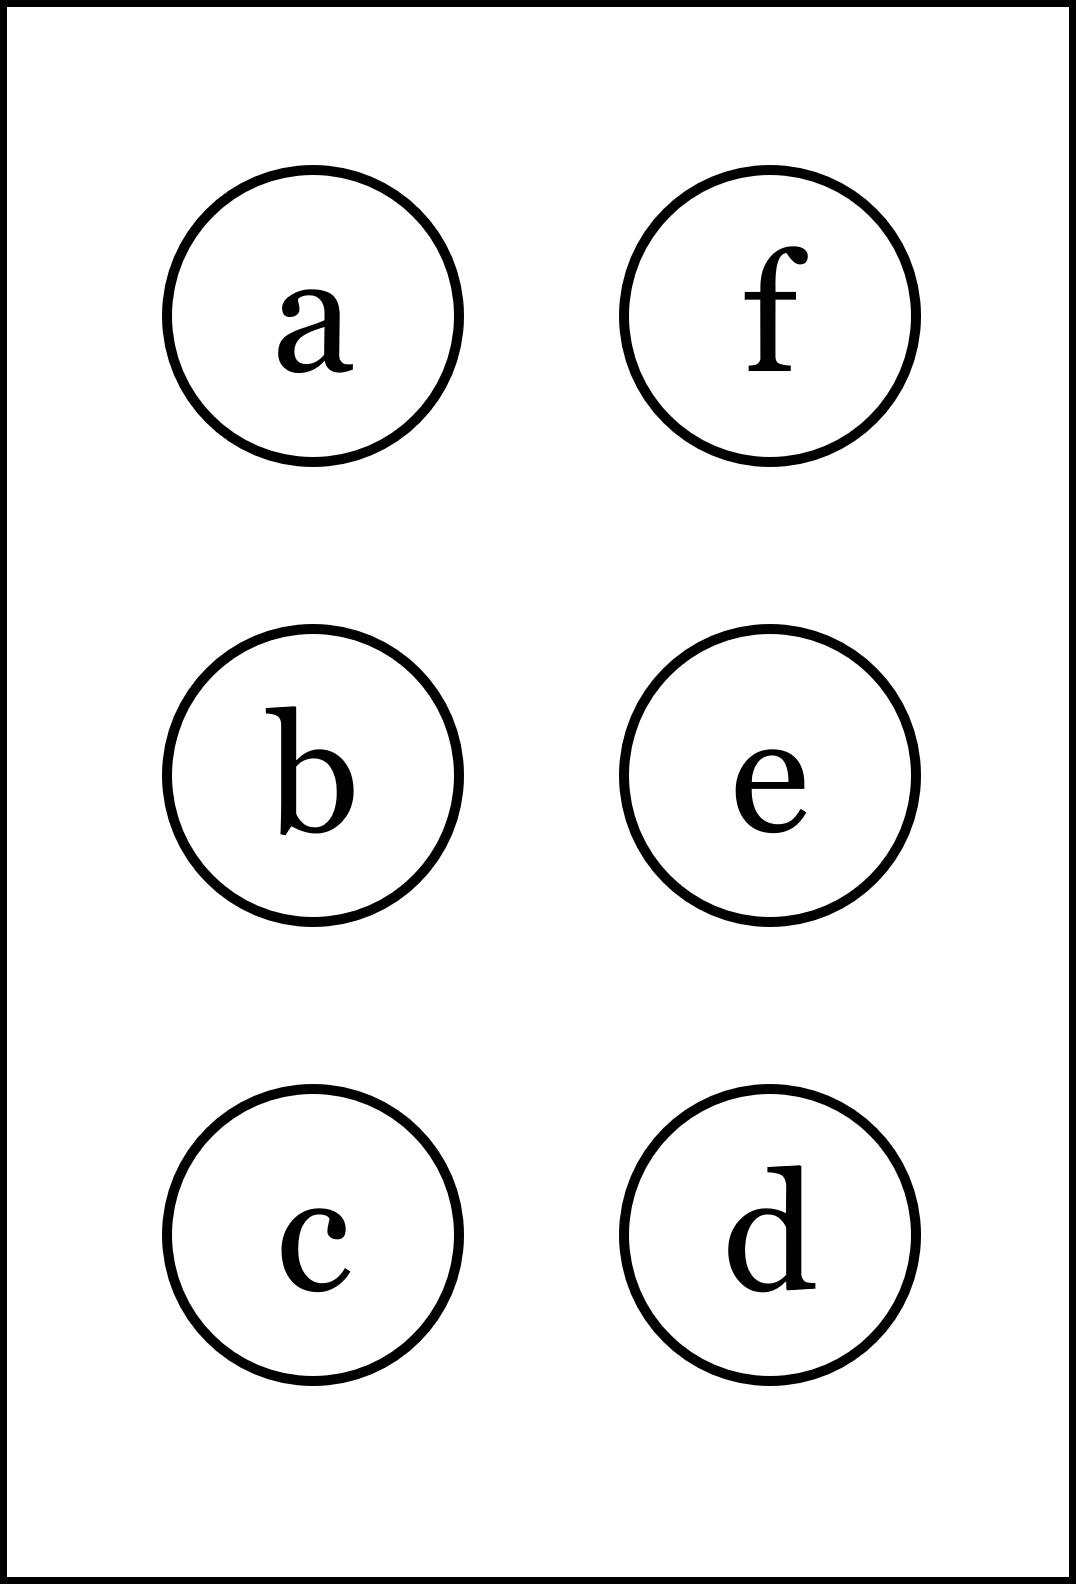
\includegraphics[height=40mm]{../images/braille.png}
{\small Písmeno Braillovej abecedy}
\end{center}
\end{minipage}
\end{center}
\end{minipage}
&
\begin{minipage}[c][104.5mm][t]{0.5\linewidth}
\begin{center}
\vspace{7mm}
{\huge Odmocniny a limity, skupina \textit{Kappa $\kappa$} -\romannumeral2}\\[5mm]
\textit{Jméno:}\phantom{xxxxxxxxxxxxxxxxxxxxxxxxxxxxxxxxxxxxxxxxxxxxxxxxxxxxxxxxxxxxxxxxx}\\[5mm]
\begin{minipage}{0.95\linewidth}
\begin{center}
V \textbf{(a)} a \textbf{(b)} \textbf{uprav výrazy}, v \textbf{(c)} a \textbf{(d)} \textbf{vypočítaj limity}.\\Pokud se výsledky shodujú s tými za otazníky, tak napravo obarvi\\příslušející kroužek načerno. \textbf{Spolu odevzdejte výsledné slovo}.
\end{center}
\end{minipage}
\\[1mm]
\begin{minipage}{0.79\linewidth}
\begin{center}
\begin{varwidth}{\linewidth}
\begin{enumerate}
\small
\item $\sqrt[4]{\left(\cfrac{x^{-1}\;x^{1}}{x^{\nicefrac{-5}{4}}}\right)^{2}}$\quad \dotfill\; ???\;\dotfill \quad $x^{\nicefrac{5}{8}}$
\item {\footnotesize{\scriptsize$\big(\sqrt{x+5y}+\sqrt{x-5y}\big)^2-\big(\sqrt{x+5y}-\sqrt{x-5y}\big)^2$}\quad \dotfill\; ???\;\dotfill \quad $4\sqrt{x^2-5y^2}$}
\item $\lim\limits_{n\to\infty}\cfrac{n^{-1/2}}{\sqrt{4n-6}-\sqrt{4n-8}}$\quad \dotfill\; ???\;\dotfill \quad $2$
\item $\lim\limits_{n\to\infty}2n\cfrac{\sqrt{16n^2-2n-6}-\sqrt{16n^2+4}}{\sqrt{25n^2+7n-1}}$\quad \dotfill\; ???\;\dotfill \quad $\nicefrac{-1}{10}$
\item \quad \dotfill\; ???\;\dotfill \quad nebarvi
\item \quad \dotfill\; ???\;\dotfill \quad nebarvi
\end{enumerate}
\end{varwidth}
\end{center}
\end{minipage}
\begin{minipage}{0.20\linewidth}
\begin{center}
{\Huge\bfseries 2.} \\[2mm]
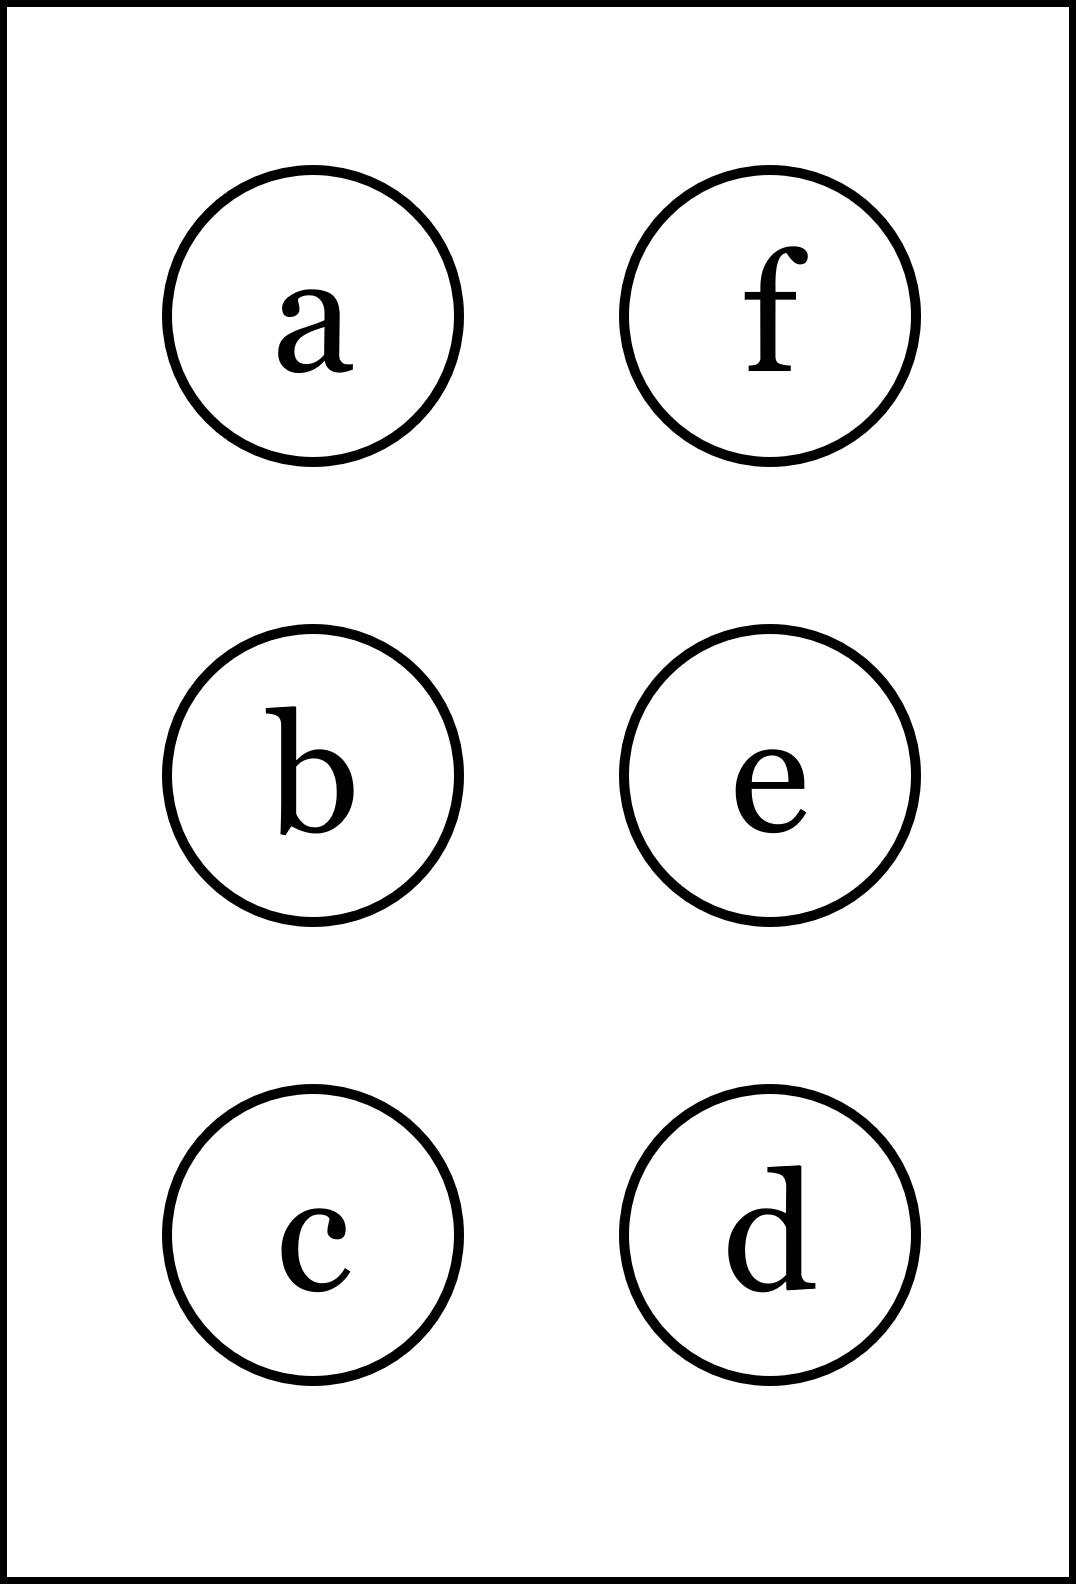
\includegraphics[height=40mm]{../images/braille.png}
{\small Písmeno Braillovej abecedy}
\end{center}
\end{minipage}
\end{center}
\end{minipage}
\\ \hdashline
\begin{minipage}[c][104.5mm][t]{0.5\linewidth}
\begin{center}
\vspace{7mm}
{\huge Odmocniny a limity, skupina \textit{Kappa $\kappa$} -\romannumeral3}\\[5mm]
\textit{Jméno:}\phantom{xxxxxxxxxxxxxxxxxxxxxxxxxxxxxxxxxxxxxxxxxxxxxxxxxxxxxxxxxxxxxxxxx}\\[5mm]
\begin{minipage}{0.95\linewidth}
\begin{center}
V \textbf{(a)} a \textbf{(b)} \textbf{uprav výrazy}, v \textbf{(c)} a \textbf{(d)} \textbf{vypočítaj limity}.\\Pokud se výsledky shodujú s tými za otazníky, tak napravo obarvi\\příslušející kroužek načerno. \textbf{Spolu odevzdejte výsledné slovo}.
\end{center}
\end{minipage}
\\[1mm]
\begin{minipage}{0.79\linewidth}
\begin{center}
\begin{varwidth}{\linewidth}
\begin{enumerate}
\small
\item $\sqrt[5]{\left(\cfrac{x^{\nicefrac{3}{2}}\;x^{3}}{x^{-1}}\right)^{2}}$\quad \dotfill\; ???\;\dotfill \quad $x^{\nicefrac{11}{5}}$
\item {\footnotesize{\scriptsize$\big(\sqrt{8x+24y}+\sqrt{8x-24y}\big)^2-\big(\sqrt{8x+24y}-\sqrt{8x-24y}\big)^2$}\quad \dotfill\; ???\;\dotfill \quad $32\sqrt{x^2-9y^2}$}
\item $\lim\limits_{n\to\infty}\cfrac{n^{-1/2}}{\sqrt{4n+2}-\sqrt{4n+1}}$\quad \dotfill\; ???\;\dotfill \quad $\infty$
\item $\lim\limits_{n\to\infty}7n\cfrac{\sqrt{n^2-3n+1}-\sqrt{n^2-3}}{\sqrt{36n^2-n+3}}$\quad \dotfill\; ???\;\dotfill \quad $\nicefrac{-7}{2}$
\item \quad \dotfill\; ???\;\dotfill \quad nebarvi
\item \quad \dotfill\; ???\;\dotfill \quad nebarvi
\end{enumerate}
\end{varwidth}
\end{center}
\end{minipage}
\begin{minipage}{0.20\linewidth}
\begin{center}
{\Huge\bfseries 3.} \\[2mm]
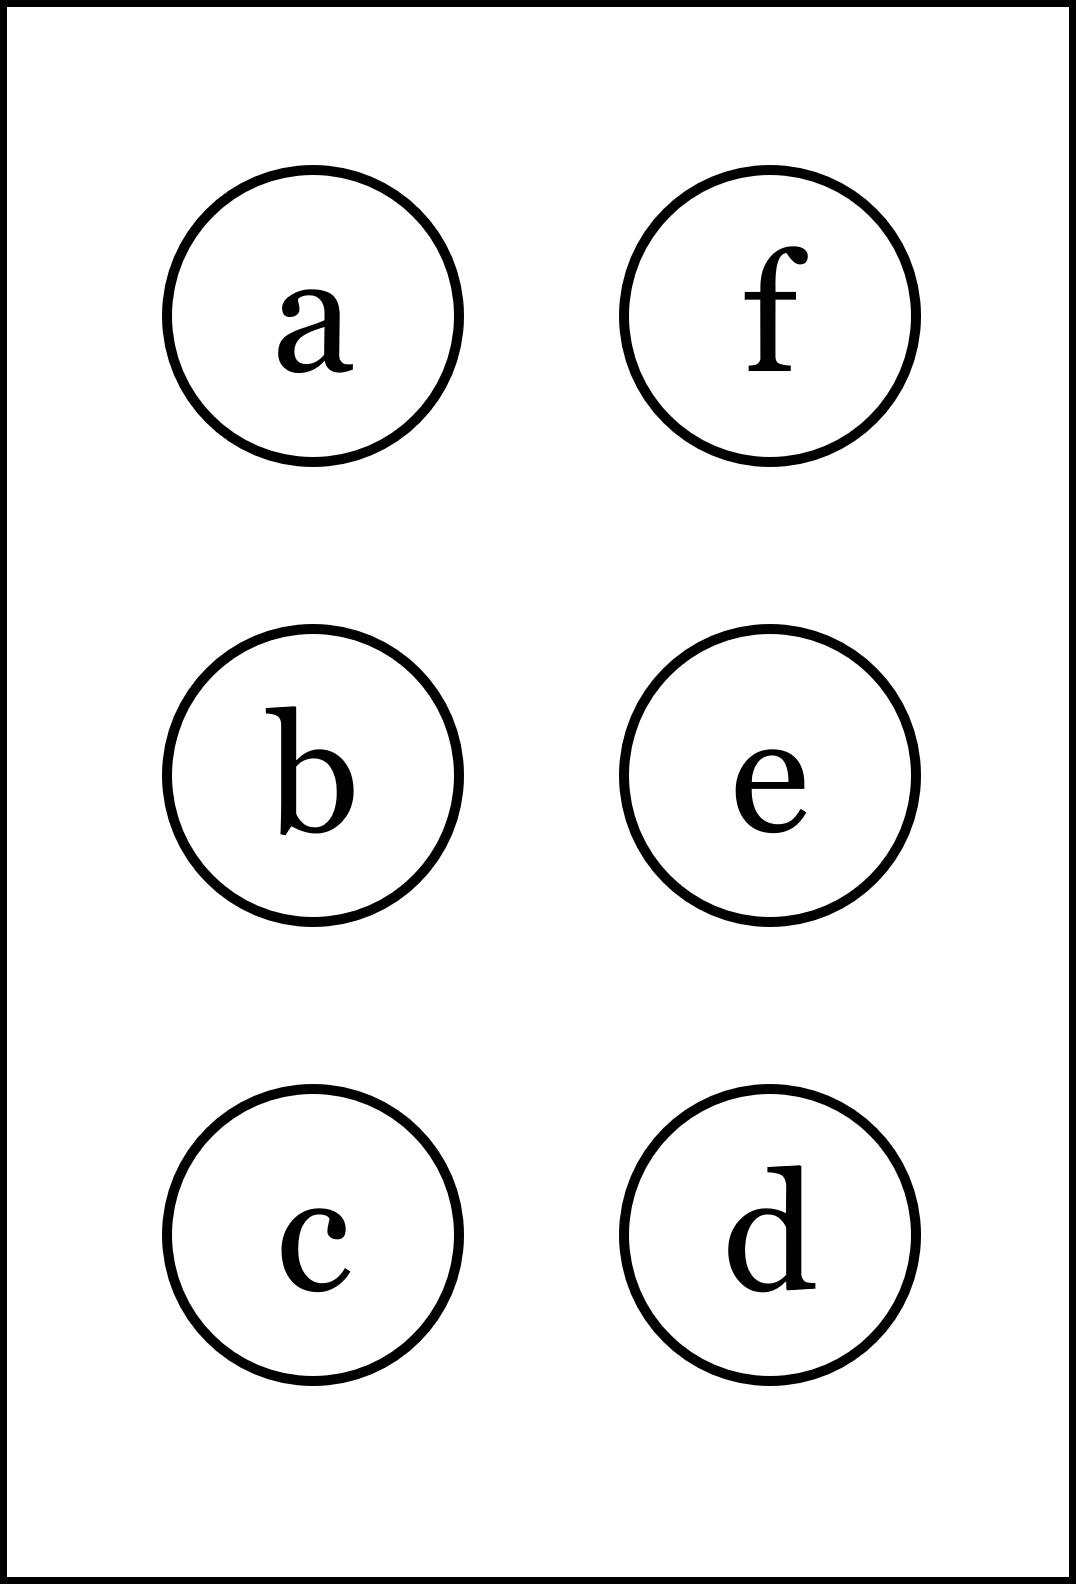
\includegraphics[height=40mm]{../images/braille.png}
{\small Písmeno Braillovej abecedy}
\end{center}
\end{minipage}
\end{center}
\end{minipage}
&
\begin{minipage}[c][104.5mm][t]{0.5\linewidth}
\begin{center}
\vspace{7mm}
{\huge Odmocniny a limity, skupina \textit{Kappa $\kappa$} -\romannumeral4}\\[5mm]
\textit{Jméno:}\phantom{xxxxxxxxxxxxxxxxxxxxxxxxxxxxxxxxxxxxxxxxxxxxxxxxxxxxxxxxxxxxxxxxx}\\[5mm]
\begin{minipage}{0.95\linewidth}
\begin{center}
V \textbf{(a)} a \textbf{(b)} \textbf{uprav výrazy}, v \textbf{(c)} a \textbf{(d)} \textbf{vypočítaj limity}.\\Pokud se výsledky shodujú s tými za otazníky, tak napravo obarvi\\příslušející kroužek načerno. \textbf{Spolu odevzdejte výsledné slovo}.
\end{center}
\end{minipage}
\\[1mm]
\begin{minipage}{0.79\linewidth}
\begin{center}
\begin{varwidth}{\linewidth}
\begin{enumerate}
\small
\item $\sqrt[3]{\left(\cfrac{x^{\nicefrac{-9}{2}}\;x^{\nicefrac{5}{2}}}{x^{\nicefrac{3}{2}}}\right)^{2}}$\quad \dotfill\; ???\;\dotfill \quad $x^{\nicefrac{-7}{3}}$
\item {\footnotesize{\scriptsize$\big(\sqrt{6x+30y}+\sqrt{6x-30y}\big)^2-\big(\sqrt{6x+30y}-\sqrt{6x-30y}\big)^2$}\quad \dotfill\; ???\;\dotfill \quad $24\sqrt{x^2-5y^2}$}
\item $\lim\limits_{n\to\infty}\cfrac{n^{-1/2}}{\sqrt{4n+2}-\sqrt{4n-1}}$\quad \dotfill\; ???\;\dotfill \quad $\nicefrac{4}{3}$
\item $\lim\limits_{n\to\infty}4n\cfrac{\sqrt{36n^2+7n-6}-\sqrt{36n^2+2}}{\sqrt{n^2+5n+7}}$\quad \dotfill\; ???\;\dotfill \quad $\nicefrac{7}{3}$
\item \quad \dotfill\; ???\;\dotfill \quad vybarvi
\item \quad \dotfill\; ???\;\dotfill \quad vybarvi
\end{enumerate}
\end{varwidth}
\end{center}
\end{minipage}
\begin{minipage}{0.20\linewidth}
\begin{center}
{\Huge\bfseries 4.} \\[2mm]
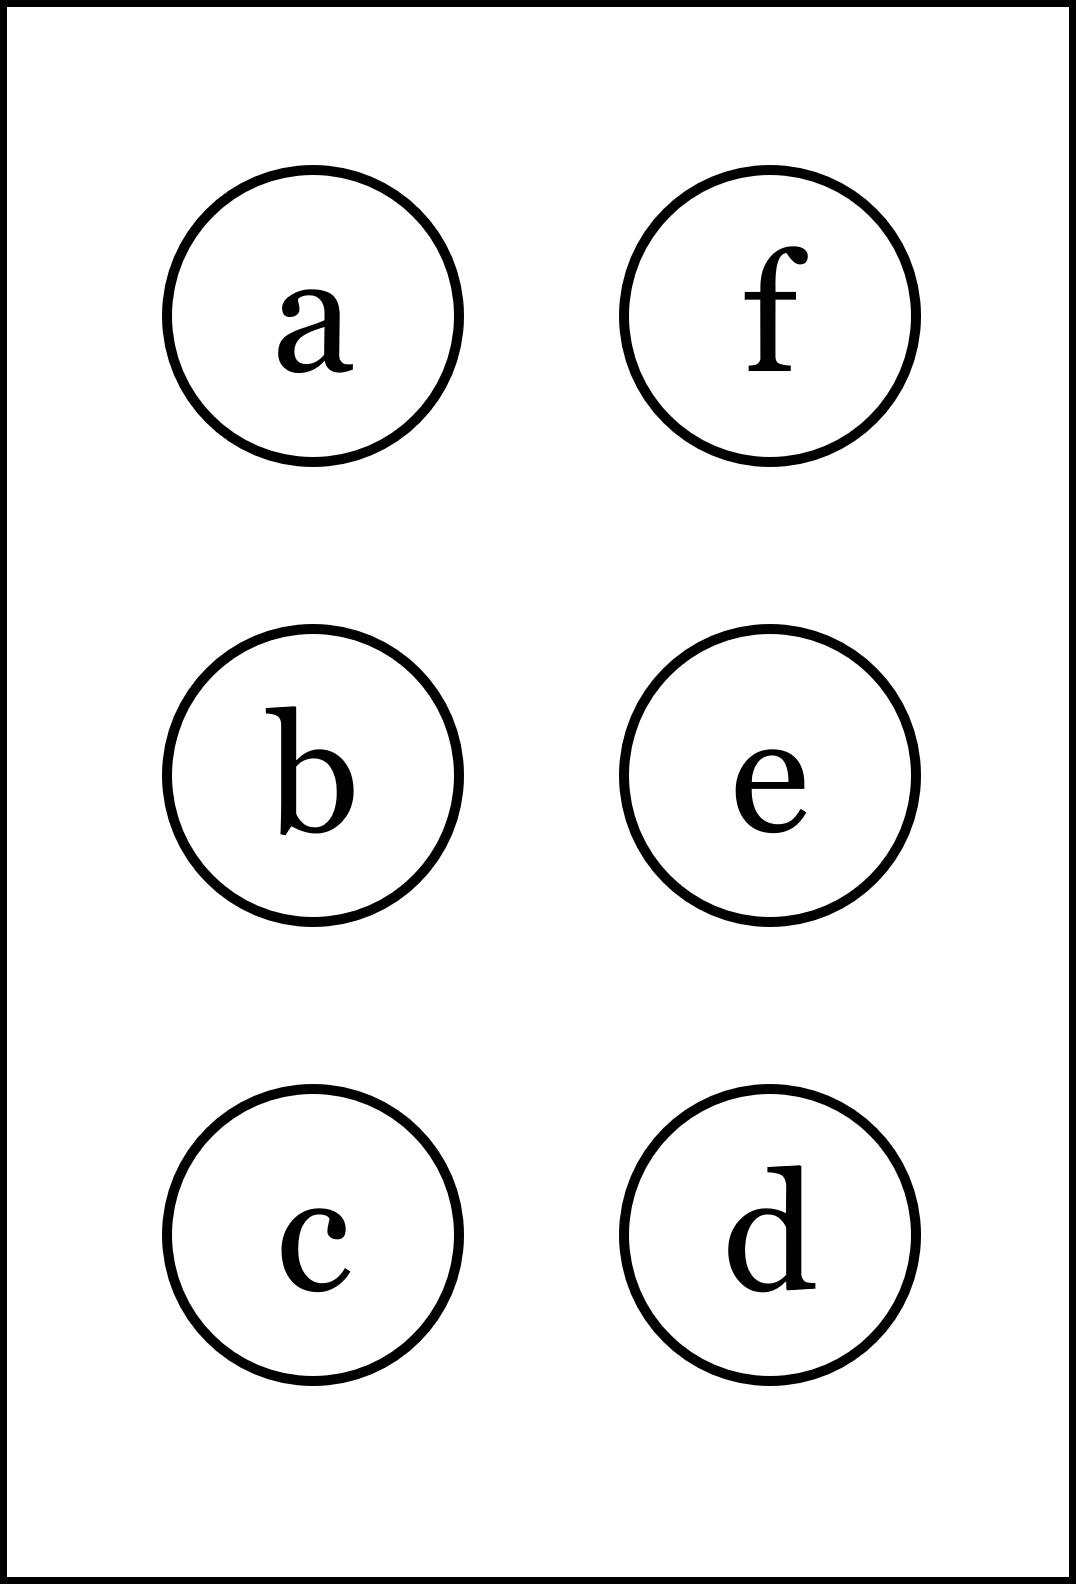
\includegraphics[height=40mm]{../images/braille.png}
{\small Písmeno Braillovej abecedy}
\end{center}
\end{minipage}
\end{center}
\end{minipage}
%
\end{tabular}
\newpage
\thispagestyle{empty}
\begin{tabular}{c:c}
\begin{minipage}[c][104.5mm][t]{0.5\linewidth}
\begin{center}
\vspace{7mm}
{\huge Odmocniny a limity, skupina \textit{Lambda $\lambda$} -\romannumeral1}\\[5mm]
\textit{Jméno:}\phantom{xxxxxxxxxxxxxxxxxxxxxxxxxxxxxxxxxxxxxxxxxxxxxxxxxxxxxxxxxxxxxxxxx}\\[5mm]
\begin{minipage}{0.95\linewidth}
\begin{center}
V \textbf{(a)} a \textbf{(b)} \textbf{uprav výrazy}, v \textbf{(c)} a \textbf{(d)} \textbf{vypočítaj limity}.\\Pokud se výsledky shodujú s tými za otazníky, tak napravo obarvi\\příslušející kroužek načerno. \textbf{Spolu odevzdejte výsledné slovo}.
\end{center}
\end{minipage}
\\[1mm]
\begin{minipage}{0.79\linewidth}
\begin{center}
\begin{varwidth}{\linewidth}
\begin{enumerate}
\small
\item $\sqrt[4]{\left(\cfrac{x^{\nicefrac{-3}{4}}\;x^{\nicefrac{-2}{3}}}{x^{1}}\right)^{3}}$\quad \dotfill\; ???\;\dotfill \quad $x^{\nicefrac{-29}{16}}$
\item {\footnotesize{\scriptsize$\big(\sqrt{5x-15y}+\sqrt{5x+15y}\big)^2-\big(\sqrt{5x-15y}-\sqrt{5x+15y}\big)^2$}\quad \dotfill\; ???\;\dotfill \quad $20\sqrt{x^2+3y^2}$}
\item $\lim\limits_{n\to\infty}\cfrac{n^{-1/2}}{\sqrt{16n+2}-\sqrt{16n+1}}$\quad \dotfill\; ???\;\dotfill \quad $\infty$
\item $\lim\limits_{n\to\infty}3n\cfrac{\sqrt{25n^2-n+3}-\sqrt{25n^2+1}}{\sqrt{4n^2+3n+4}}$\quad \dotfill\; ???\;\dotfill \quad $\nicefrac{-3}{10}$
\item \quad \dotfill\; ???\;\dotfill \quad vybarvi
\item \quad \dotfill\; ???\;\dotfill \quad nebarvi
\end{enumerate}
\end{varwidth}
\end{center}
\end{minipage}
\begin{minipage}{0.20\linewidth}
\begin{center}
{\Huge\bfseries 1.} \\[2mm]
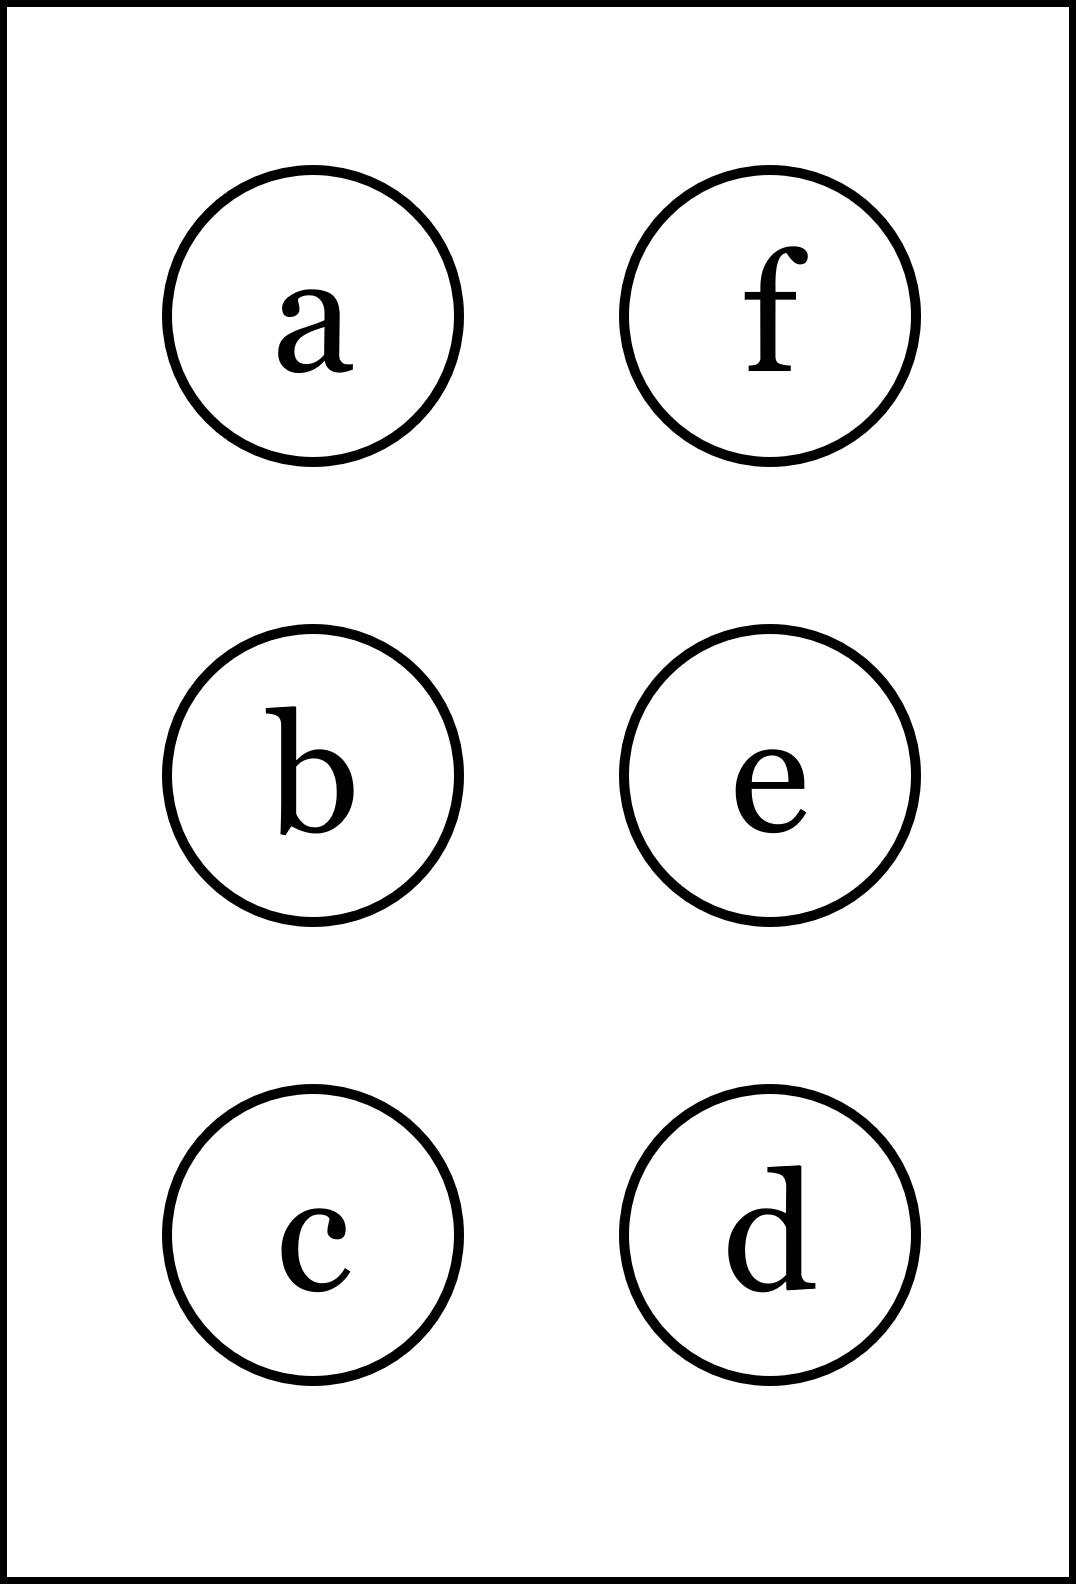
\includegraphics[height=40mm]{../images/braille.png}
{\small Písmeno Braillovej abecedy}
\end{center}
\end{minipage}
\end{center}
\end{minipage}
&
\begin{minipage}[c][104.5mm][t]{0.5\linewidth}
\begin{center}
\vspace{7mm}
{\huge Odmocniny a limity, skupina \textit{Lambda $\lambda$} -\romannumeral2}\\[5mm]
\textit{Jméno:}\phantom{xxxxxxxxxxxxxxxxxxxxxxxxxxxxxxxxxxxxxxxxxxxxxxxxxxxxxxxxxxxxxxxxx}\\[5mm]
\begin{minipage}{0.95\linewidth}
\begin{center}
V \textbf{(a)} a \textbf{(b)} \textbf{uprav výrazy}, v \textbf{(c)} a \textbf{(d)} \textbf{vypočítaj limity}.\\Pokud se výsledky shodujú s tými za otazníky, tak napravo obarvi\\příslušející kroužek načerno. \textbf{Spolu odevzdejte výsledné slovo}.
\end{center}
\end{minipage}
\\[1mm]
\begin{minipage}{0.79\linewidth}
\begin{center}
\begin{varwidth}{\linewidth}
\begin{enumerate}
\small
\item $\sqrt[5]{\left(\cfrac{x^{-1}\;x^{2}}{x^{\nicefrac{-1}{2}}}\right)^{4}}$\quad \dotfill\; ???\;\dotfill \quad $x^{\nicefrac{6}{5}}$
\item {\footnotesize{\scriptsize$\big(\sqrt{6x+30y}+\sqrt{6x-30y}\big)^2-\big(\sqrt{6x+30y}-\sqrt{6x-30y}\big)^2$}\quad \dotfill\; ???\;\dotfill \quad $24\sqrt{x^2-5y^2}$}
\item $\lim\limits_{n\to\infty}\cfrac{n^{-1/2}}{\sqrt{n+3}-\sqrt{n+2}}$\quad \dotfill\; ???\;\dotfill \quad $2$
\item $\lim\limits_{n\to\infty}2n\cfrac{\sqrt{49n^2-4n+5}-\sqrt{49n^2+5}}{\sqrt{25n^2+8n-2}}$\quad \dotfill\; ???\;\dotfill \quad $\nicefrac{-4}{35}$
\item \quad \dotfill\; ???\;\dotfill \quad nebarvi
\item \quad \dotfill\; ???\;\dotfill \quad nebarvi
\end{enumerate}
\end{varwidth}
\end{center}
\end{minipage}
\begin{minipage}{0.20\linewidth}
\begin{center}
{\Huge\bfseries 2.} \\[2mm]
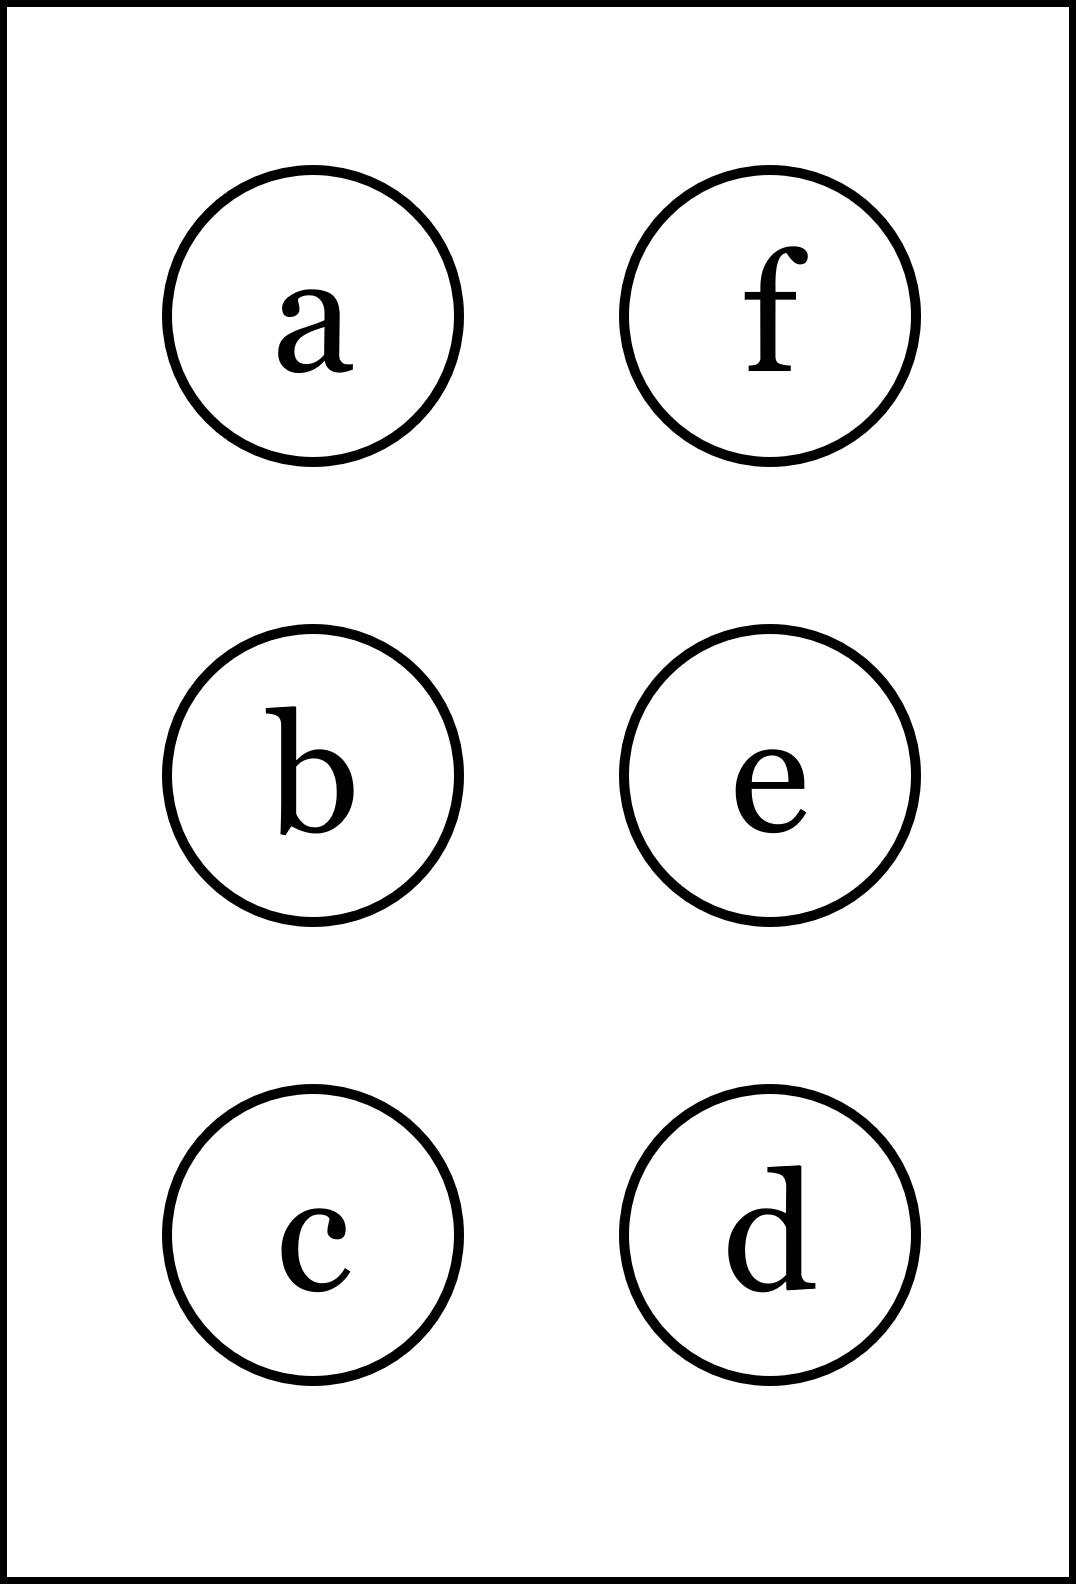
\includegraphics[height=40mm]{../images/braille.png}
{\small Písmeno Braillovej abecedy}
\end{center}
\end{minipage}
\end{center}
\end{minipage}
\\ \hdashline
\begin{minipage}[c][104.5mm][t]{0.5\linewidth}
\begin{center}
\vspace{7mm}
{\huge Odmocniny a limity, skupina \textit{Lambda $\lambda$} -\romannumeral3}\\[5mm]
\textit{Jméno:}\phantom{xxxxxxxxxxxxxxxxxxxxxxxxxxxxxxxxxxxxxxxxxxxxxxxxxxxxxxxxxxxxxxxxx}\\[5mm]
\begin{minipage}{0.95\linewidth}
\begin{center}
V \textbf{(a)} a \textbf{(b)} \textbf{uprav výrazy}, v \textbf{(c)} a \textbf{(d)} \textbf{vypočítaj limity}.\\Pokud se výsledky shodujú s tými za otazníky, tak napravo obarvi\\příslušející kroužek načerno. \textbf{Spolu odevzdejte výsledné slovo}.
\end{center}
\end{minipage}
\\[1mm]
\begin{minipage}{0.79\linewidth}
\begin{center}
\begin{varwidth}{\linewidth}
\begin{enumerate}
\small
\item $\sqrt[2]{\left(\cfrac{x^{\nicefrac{-3}{2}}\;x^{-7}}{x^{\nicefrac{5}{2}}}\right)^{2}}$\quad \dotfill\; ???\;\dotfill \quad $x^{-11}$
\item {\footnotesize{\scriptsize$\big(\sqrt{5x-5y}+\sqrt{5x+5y}\big)^2-\big(\sqrt{5x-5y}-\sqrt{5x+5y}\big)^2$}\quad \dotfill\; ???\;\dotfill \quad $20\sqrt{x^2-y^2}$}
\item $\lim\limits_{n\to\infty}\cfrac{n^{-1/2}}{\sqrt{9n-4}-\sqrt{9n-1}}$\quad \dotfill\; ???\;\dotfill \quad $-2$
\item $\lim\limits_{n\to\infty}7n\cfrac{\sqrt{9n^2+2n-2}-\sqrt{9n^2-7}}{\sqrt{25n^2+2n-2}}$\quad \dotfill\; ???\;\dotfill \quad $\nicefrac{14}{15}$
\item \quad \dotfill\; ???\;\dotfill \quad vybarvi
\item \quad \dotfill\; ???\;\dotfill \quad nebarvi
\end{enumerate}
\end{varwidth}
\end{center}
\end{minipage}
\begin{minipage}{0.20\linewidth}
\begin{center}
{\Huge\bfseries 3.} \\[2mm]
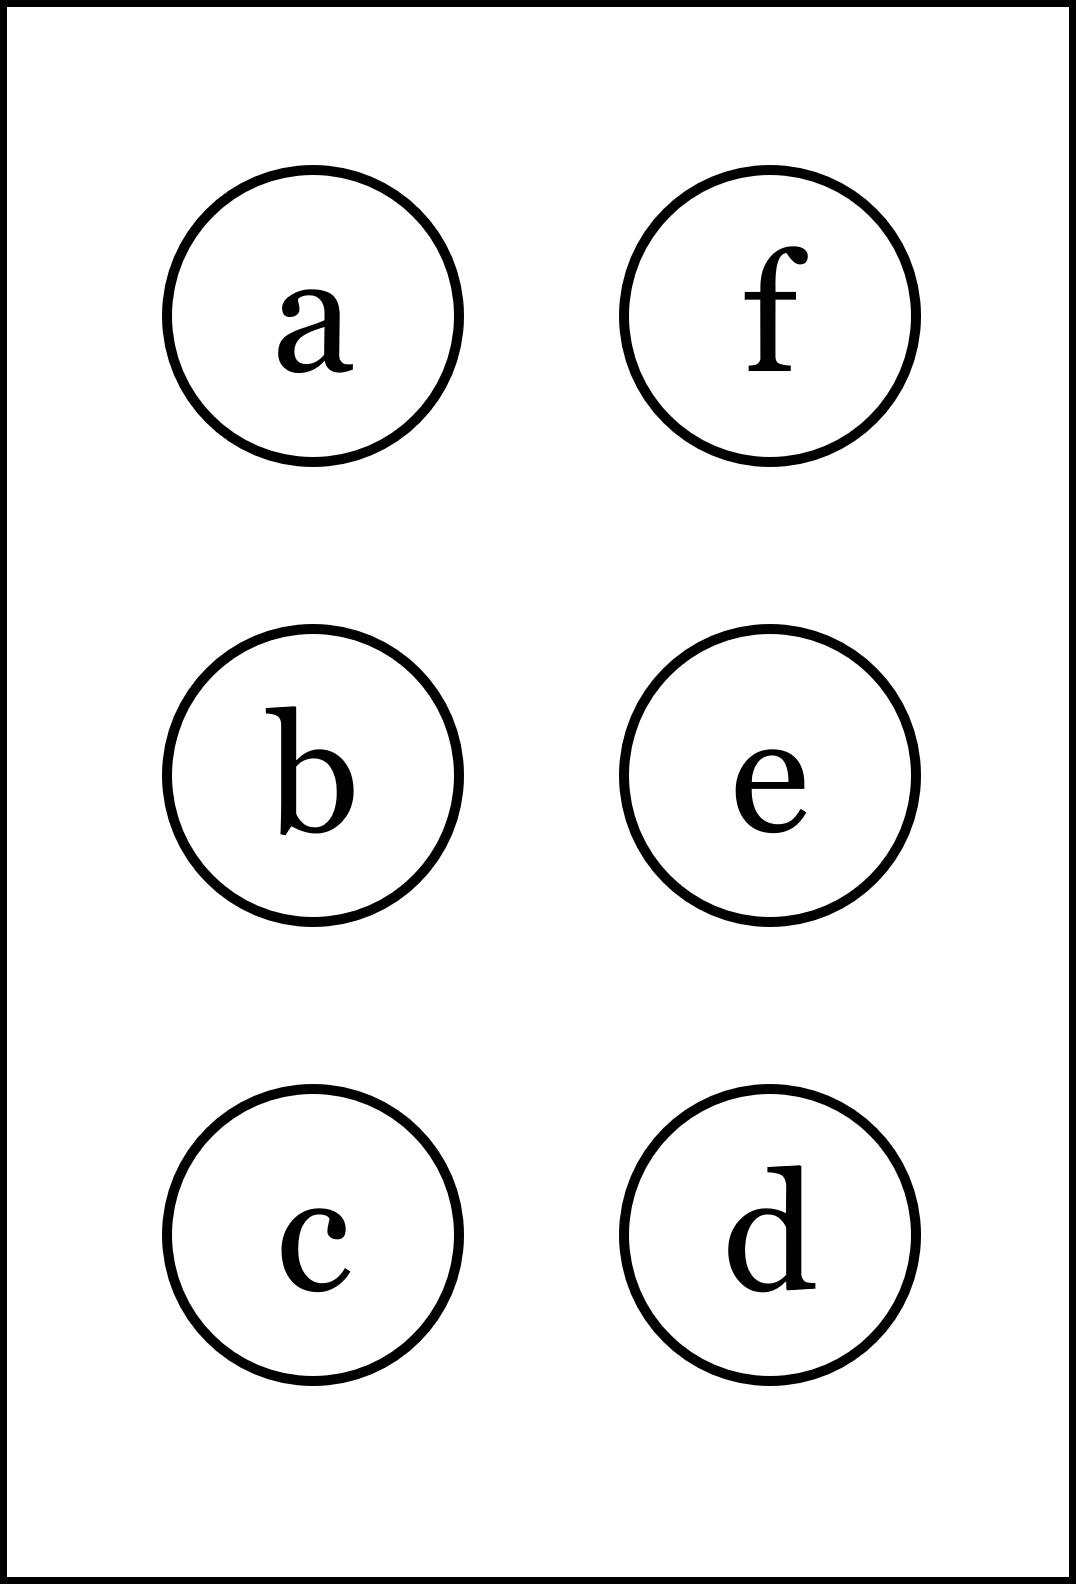
\includegraphics[height=40mm]{../images/braille.png}
{\small Písmeno Braillovej abecedy}
\end{center}
\end{minipage}
\end{center}
\end{minipage}
&
\begin{minipage}[c][104.5mm][t]{0.5\linewidth}
\begin{center}
\vspace{7mm}
{\huge Odmocniny a limity, skupina \textit{Lambda $\lambda$} -\romannumeral4}\\[5mm]
\textit{Jméno:}\phantom{xxxxxxxxxxxxxxxxxxxxxxxxxxxxxxxxxxxxxxxxxxxxxxxxxxxxxxxxxxxxxxxxx}\\[5mm]
\begin{minipage}{0.95\linewidth}
\begin{center}
V \textbf{(a)} a \textbf{(b)} \textbf{uprav výrazy}, v \textbf{(c)} a \textbf{(d)} \textbf{vypočítaj limity}.\\Pokud se výsledky shodujú s tými za otazníky, tak napravo obarvi\\příslušející kroužek načerno. \textbf{Spolu odevzdejte výsledné slovo}.
\end{center}
\end{minipage}
\\[1mm]
\begin{minipage}{0.79\linewidth}
\begin{center}
\begin{varwidth}{\linewidth}
\begin{enumerate}
\small
\item $\sqrt[1]{\left(\cfrac{x^{1}\;x^{\nicefrac{1}{7}}}{x^{1}}\right)^{5}}$\quad \dotfill\; ???\;\dotfill \quad $x^{\nicefrac{5}{7}}$
\item {\footnotesize{\scriptsize$\big(\sqrt{5x-25y}+\sqrt{5x+25y}\big)^2-\big(\sqrt{5x-25y}-\sqrt{5x+25y}\big)^2$}\quad \dotfill\; ???\;\dotfill \quad $20\sqrt{x^2+5y^2}$}
\item $\lim\limits_{n\to\infty}\cfrac{n^{-1/2}}{\sqrt{n+8}-\sqrt{n-5}}$\quad \dotfill\; ???\;\dotfill \quad $\nicefrac{2}{13}$
\item $\lim\limits_{n\to\infty}5n\cfrac{\sqrt{n^2+4n-1}-\sqrt{n^2-9}}{\sqrt{4n^2-2n+2}}$\quad \dotfill\; ???\;\dotfill \quad $10$
\item \quad \dotfill\; ???\;\dotfill \quad vybarvi
\item \quad \dotfill\; ???\;\dotfill \quad nebarvi
\end{enumerate}
\end{varwidth}
\end{center}
\end{minipage}
\begin{minipage}{0.20\linewidth}
\begin{center}
{\Huge\bfseries 4.} \\[2mm]
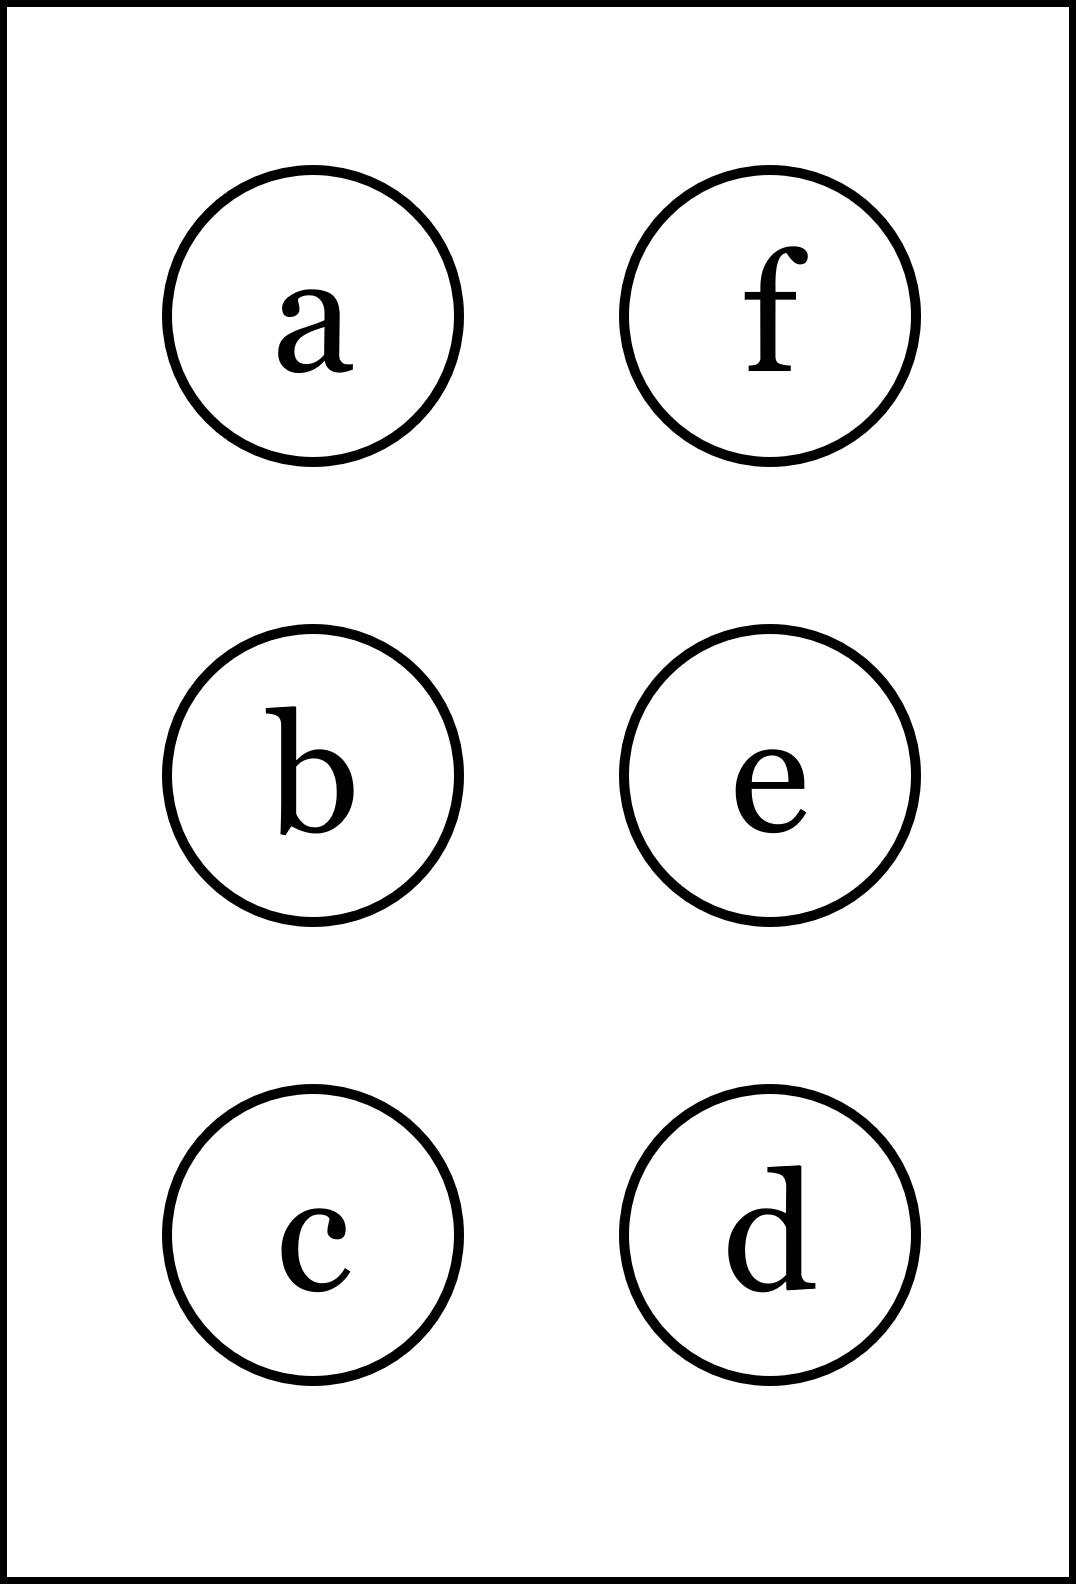
\includegraphics[height=40mm]{../images/braille.png}
{\small Písmeno Braillovej abecedy}
\end{center}
\end{minipage}
\end{center}
\end{minipage}
%
\end{tabular}
\newpage
\thispagestyle{empty}
\begin{tabular}{c:c}
\begin{minipage}[c][104.5mm][t]{0.5\linewidth}
\begin{center}
\vspace{7mm}
{\huge Odmocniny a limity, skupina \textit{Mu $\mu$} -\romannumeral1}\\[5mm]
\textit{Jméno:}\phantom{xxxxxxxxxxxxxxxxxxxxxxxxxxxxxxxxxxxxxxxxxxxxxxxxxxxxxxxxxxxxxxxxx}\\[5mm]
\begin{minipage}{0.95\linewidth}
\begin{center}
V \textbf{(a)} a \textbf{(b)} \textbf{uprav výrazy}, v \textbf{(c)} a \textbf{(d)} \textbf{vypočítaj limity}.\\Pokud se výsledky shodujú s tými za otazníky, tak napravo obarvi\\příslušející kroužek načerno. \textbf{Spolu odevzdejte výsledné slovo}.
\end{center}
\end{minipage}
\\[1mm]
\begin{minipage}{0.79\linewidth}
\begin{center}
\begin{varwidth}{\linewidth}
\begin{enumerate}
\small
\item $\sqrt[7]{\left(\cfrac{x^{4}\;x^{\nicefrac{-5}{4}}}{x^{-2}}\right)^{3}}$\quad \dotfill\; ???\;\dotfill \quad $x^{\nicefrac{57}{28}}$
\item {\footnotesize{\scriptsize$\big(\sqrt{x-y}+\sqrt{x+y}\big)^2-\big(\sqrt{x-y}-\sqrt{x+y}\big)^2$}\quad \dotfill\; ???\;\dotfill \quad $4\sqrt{x^2-y^2}$}
\item $\lim\limits_{n\to\infty}\cfrac{n^{-1/2}}{\sqrt{9n+3}-\sqrt{9n-5}}$\quad \dotfill\; ???\;\dotfill \quad $\nicefrac{3}{4}$
\item $\lim\limits_{n\to\infty}2n\cfrac{\sqrt{9n^2-5n-2}-\sqrt{9n^2+5}}{\sqrt{49n^2-4n-1}}$\quad \dotfill\; ???\;\dotfill \quad $\nicefrac{-5}{21}$
\item \quad \dotfill\; ???\;\dotfill \quad nebarvi
\item \quad \dotfill\; ???\;\dotfill \quad nebarvi
\end{enumerate}
\end{varwidth}
\end{center}
\end{minipage}
\begin{minipage}{0.20\linewidth}
\begin{center}
{\Huge\bfseries 1.} \\[2mm]
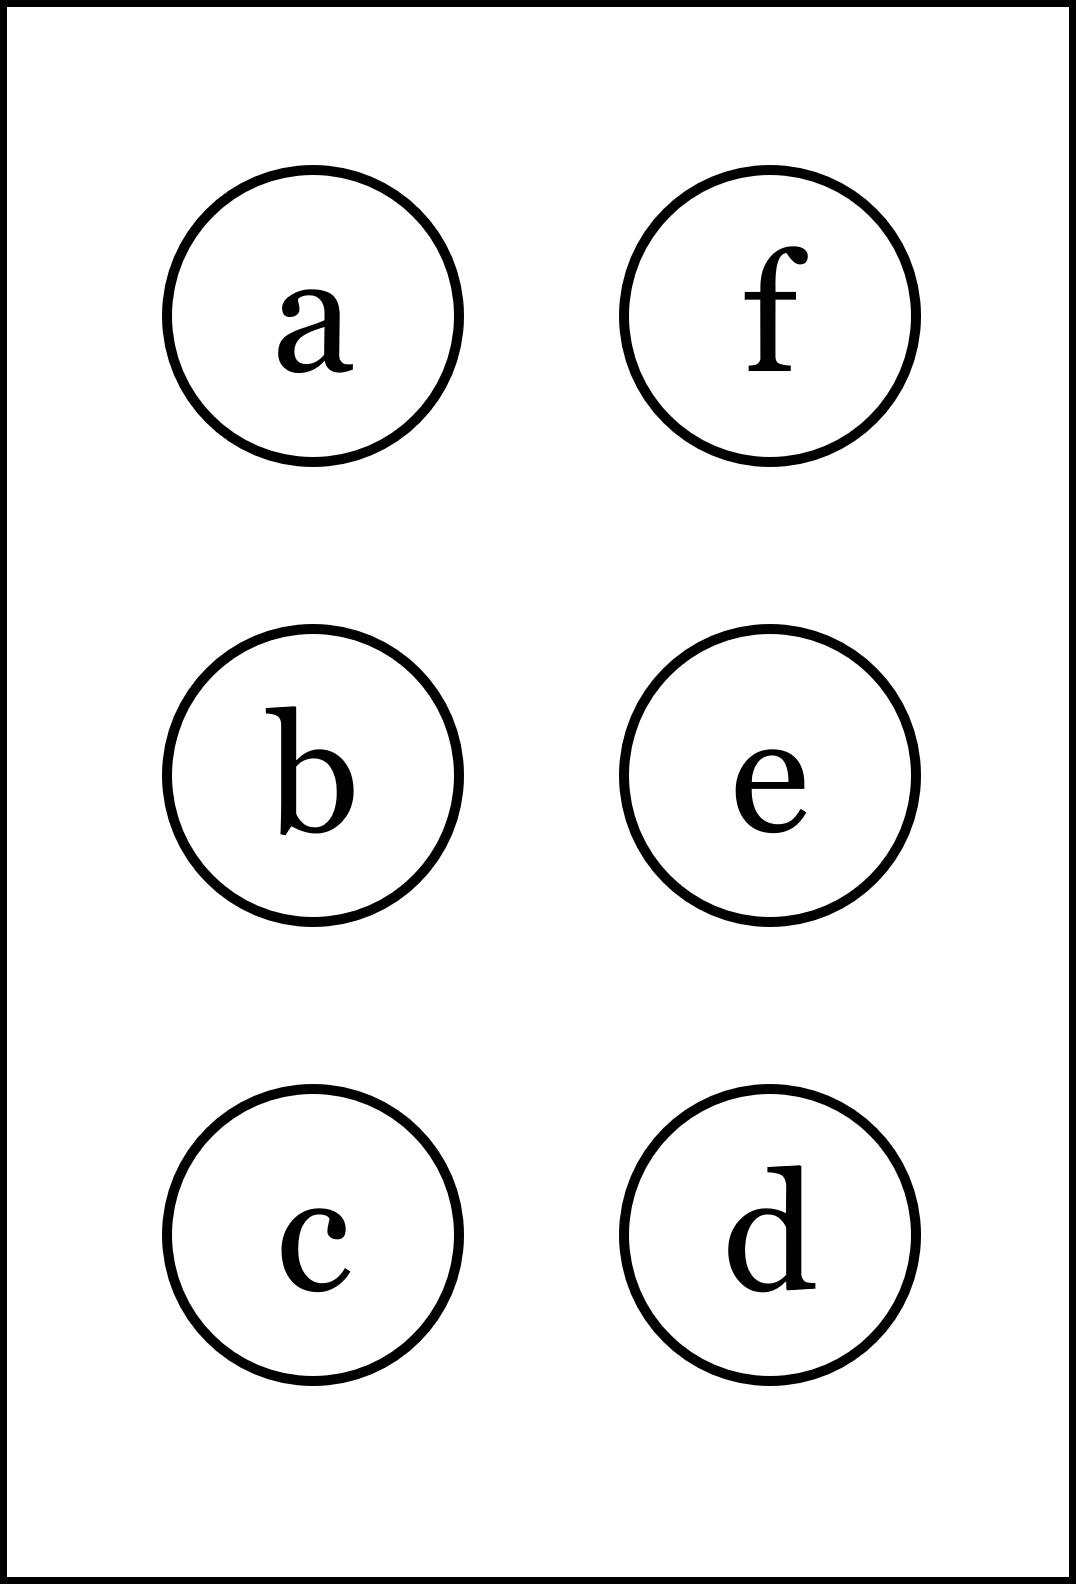
\includegraphics[height=40mm]{../images/braille.png}
{\small Písmeno Braillovej abecedy}
\end{center}
\end{minipage}
\end{center}
\end{minipage}
&
\begin{minipage}[c][104.5mm][t]{0.5\linewidth}
\begin{center}
\vspace{7mm}
{\huge Odmocniny a limity, skupina \textit{Mu $\mu$} -\romannumeral2}\\[5mm]
\textit{Jméno:}\phantom{xxxxxxxxxxxxxxxxxxxxxxxxxxxxxxxxxxxxxxxxxxxxxxxxxxxxxxxxxxxxxxxxx}\\[5mm]
\begin{minipage}{0.95\linewidth}
\begin{center}
V \textbf{(a)} a \textbf{(b)} \textbf{uprav výrazy}, v \textbf{(c)} a \textbf{(d)} \textbf{vypočítaj limity}.\\Pokud se výsledky shodujú s tými za otazníky, tak napravo obarvi\\příslušející kroužek načerno. \textbf{Spolu odevzdejte výsledné slovo}.
\end{center}
\end{minipage}
\\[1mm]
\begin{minipage}{0.79\linewidth}
\begin{center}
\begin{varwidth}{\linewidth}
\begin{enumerate}
\small
\item $\sqrt[3]{\left(\cfrac{x^{-1}\;x^{-1}}{x^{1}}\right)^{5}}$\quad \dotfill\; ???\;\dotfill \quad $x^{-5}$
\item {\footnotesize{\scriptsize$\big(\sqrt{x+y}+\sqrt{x-y}\big)^2-\big(\sqrt{x+y}-\sqrt{x-y}\big)^2$}\quad \dotfill\; ???\;\dotfill \quad $2\sqrt{x^2-y^2}$}
\item $\lim\limits_{n\to\infty}\cfrac{n^{-1/2}}{\sqrt{n-3}-\sqrt{n+1}}$\quad \dotfill\; ???\;\dotfill \quad $\nicefrac{-1}{2}$
\item $\lim\limits_{n\to\infty}2n\cfrac{\sqrt{4n^2+5n-5}-\sqrt{4n^2+5}}{\sqrt{49n^2-2n-3}}$\quad \dotfill\; ???\;\dotfill \quad $\nicefrac{5}{7}$
\item \quad \dotfill\; ???\;\dotfill \quad vybarvi
\item \quad \dotfill\; ???\;\dotfill \quad nebarvi
\end{enumerate}
\end{varwidth}
\end{center}
\end{minipage}
\begin{minipage}{0.20\linewidth}
\begin{center}
{\Huge\bfseries 2.} \\[2mm]
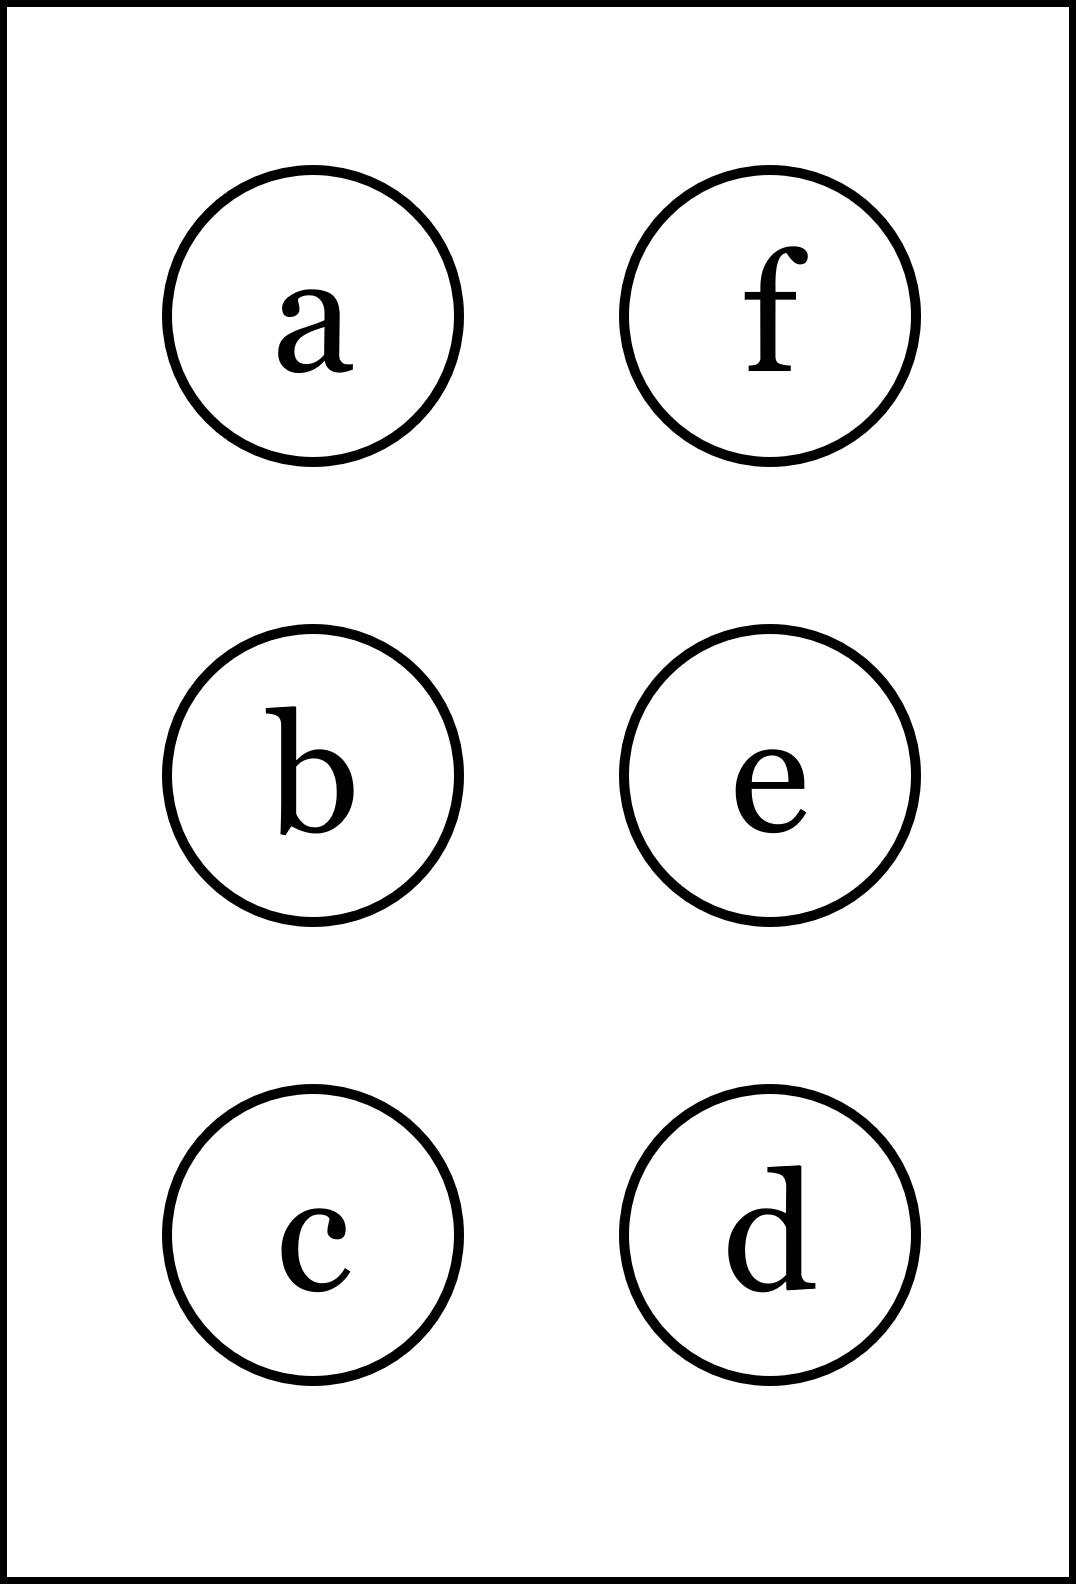
\includegraphics[height=40mm]{../images/braille.png}
{\small Písmeno Braillovej abecedy}
\end{center}
\end{minipage}
\end{center}
\end{minipage}
\\ \hdashline
\begin{minipage}[c][104.5mm][t]{0.5\linewidth}
\begin{center}
\vspace{7mm}
{\huge Odmocniny a limity, skupina \textit{Mu $\mu$} -\romannumeral3}\\[5mm]
\textit{Jméno:}\phantom{xxxxxxxxxxxxxxxxxxxxxxxxxxxxxxxxxxxxxxxxxxxxxxxxxxxxxxxxxxxxxxxxx}\\[5mm]
\begin{minipage}{0.95\linewidth}
\begin{center}
V \textbf{(a)} a \textbf{(b)} \textbf{uprav výrazy}, v \textbf{(c)} a \textbf{(d)} \textbf{vypočítaj limity}.\\Pokud se výsledky shodujú s tými za otazníky, tak napravo obarvi\\příslušející kroužek načerno. \textbf{Spolu odevzdejte výsledné slovo}.
\end{center}
\end{minipage}
\\[1mm]
\begin{minipage}{0.79\linewidth}
\begin{center}
\begin{varwidth}{\linewidth}
\begin{enumerate}
\small
\item $\sqrt[8]{\left(\cfrac{x^{6}\;x^{\nicefrac{5}{6}}}{x^{-6}}\right)^{2}}$\quad \dotfill\; ???\;\dotfill \quad $x^{\nicefrac{77}{24}}$
\item {\footnotesize{\scriptsize$\big(\sqrt{5x-20y}+\sqrt{5x+20y}\big)^2-\big(\sqrt{5x-20y}-\sqrt{5x+20y}\big)^2$}\quad \dotfill\; ???\;\dotfill \quad $20\sqrt{x^2+4y^2}$}
\item $\lim\limits_{n\to\infty}\cfrac{n^{-1/2}}{\sqrt{4n-3}-\sqrt{4n+9}}$\quad \dotfill\; ???\;\dotfill \quad $\nicefrac{2}{3}$
\item $\lim\limits_{n\to\infty}7n\cfrac{\sqrt{25n^2-2n-5}-\sqrt{25n^2+5}}{\sqrt{n^2+2n-2}}$\quad \dotfill\; ???\;\dotfill \quad $\nicefrac{-14}{5}$
\item \quad \dotfill\; ???\;\dotfill \quad vybarvi
\item \quad \dotfill\; ???\;\dotfill \quad vybarvi
\end{enumerate}
\end{varwidth}
\end{center}
\end{minipage}
\begin{minipage}{0.20\linewidth}
\begin{center}
{\Huge\bfseries 3.} \\[2mm]
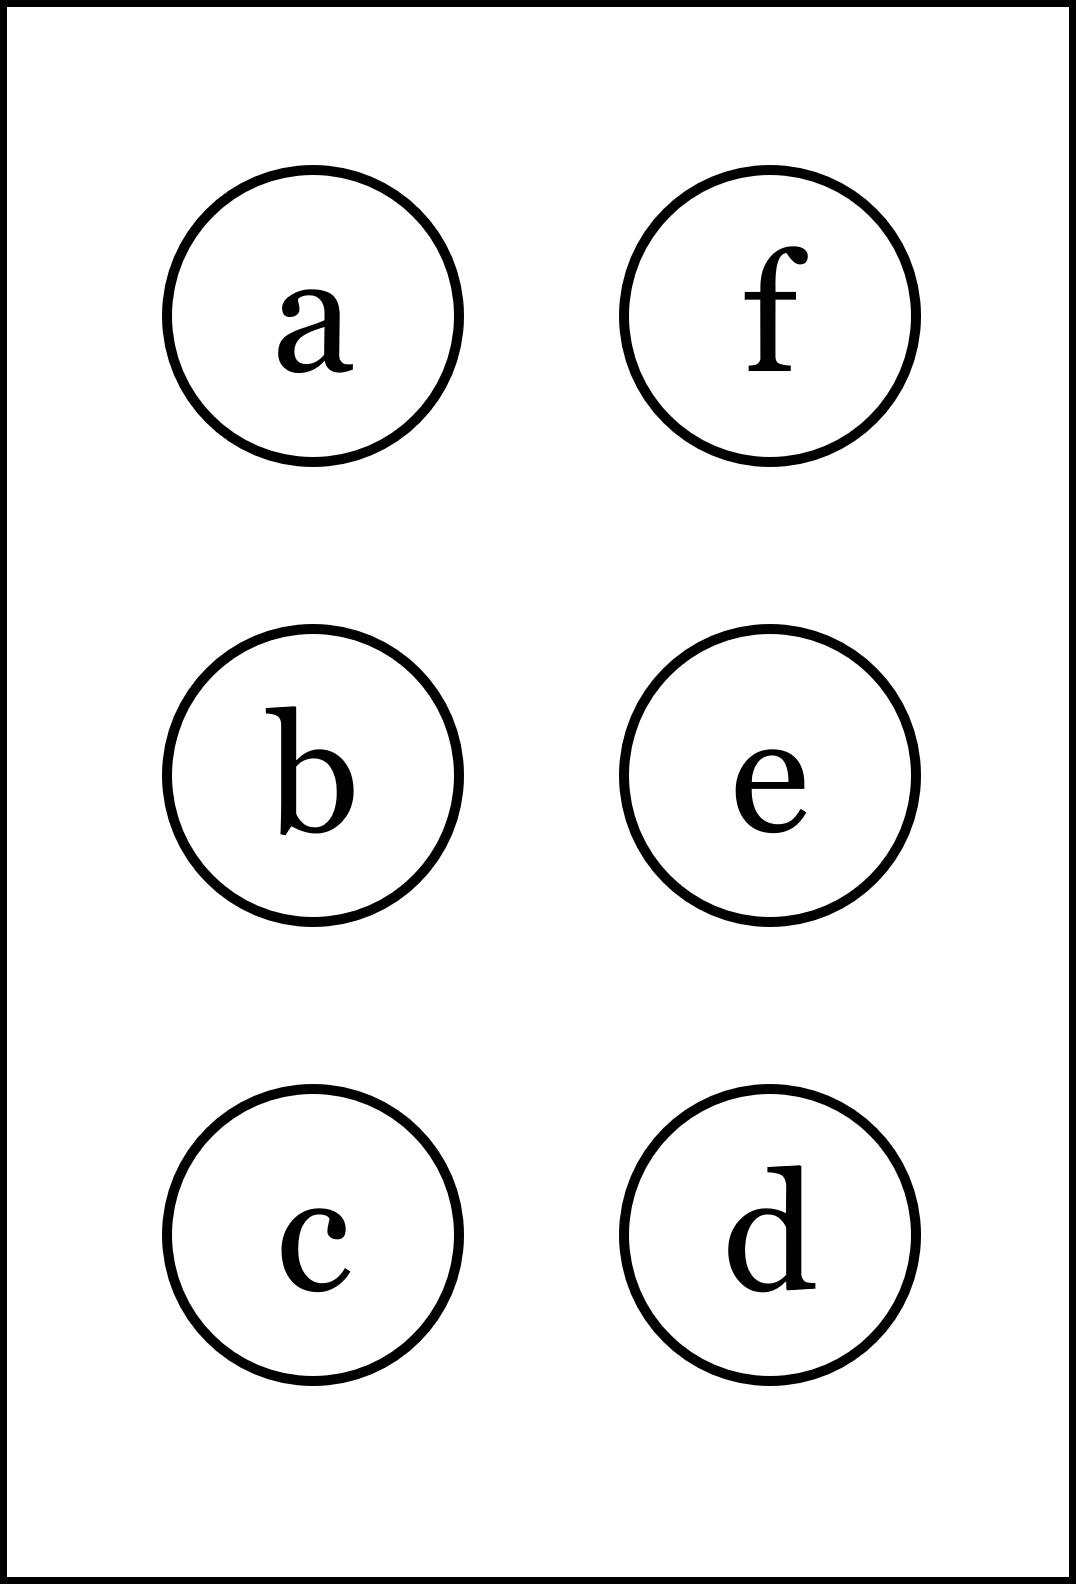
\includegraphics[height=40mm]{../images/braille.png}
{\small Písmeno Braillovej abecedy}
\end{center}
\end{minipage}
\end{center}
\end{minipage}
&
\begin{minipage}[c][104.5mm][t]{0.5\linewidth}
\begin{center}
\vspace{7mm}
{\huge Odmocniny a limity, skupina \textit{Mu $\mu$} -\romannumeral4}\\[5mm]
\textit{Jméno:}\phantom{xxxxxxxxxxxxxxxxxxxxxxxxxxxxxxxxxxxxxxxxxxxxxxxxxxxxxxxxxxxxxxxxx}\\[5mm]
\begin{minipage}{0.95\linewidth}
\begin{center}
V \textbf{(a)} a \textbf{(b)} \textbf{uprav výrazy}, v \textbf{(c)} a \textbf{(d)} \textbf{vypočítaj limity}.\\Pokud se výsledky shodujú s tými za otazníky, tak napravo obarvi\\příslušející kroužek načerno. \textbf{Spolu odevzdejte výsledné slovo}.
\end{center}
\end{minipage}
\\[1mm]
\begin{minipage}{0.79\linewidth}
\begin{center}
\begin{varwidth}{\linewidth}
\begin{enumerate}
\small
\item $\sqrt[2]{\left(\cfrac{x^{8}\;x^{1}}{x^{3}}\right)^{5}}$\quad \dotfill\; ???\;\dotfill \quad $x^{15}$
\item {\footnotesize{\scriptsize$\big(\sqrt{6x+6y}+\sqrt{6x-6y}\big)^2-\big(\sqrt{6x+6y}-\sqrt{6x-6y}\big)^2$}\quad \dotfill\; ???\;\dotfill \quad $12\sqrt{x^2-y^2}$}
\item $\lim\limits_{n\to\infty}\cfrac{n^{-1/2}}{\sqrt{49n+4}-\sqrt{49n-3}}$\quad \dotfill\; ???\;\dotfill \quad $-\infty$
\item $\lim\limits_{n\to\infty}3n\cfrac{\sqrt{64n^2+n-2}-\sqrt{64n^2-6}}{\sqrt{16n^2-3n-7}}$\quad \dotfill\; ???\;\dotfill \quad $\nicefrac{3}{32}$
\item \quad \dotfill\; ???\;\dotfill \quad nebarvi
\item \quad \dotfill\; ???\;\dotfill \quad nebarvi
\end{enumerate}
\end{varwidth}
\end{center}
\end{minipage}
\begin{minipage}{0.20\linewidth}
\begin{center}
{\Huge\bfseries 4.} \\[2mm]
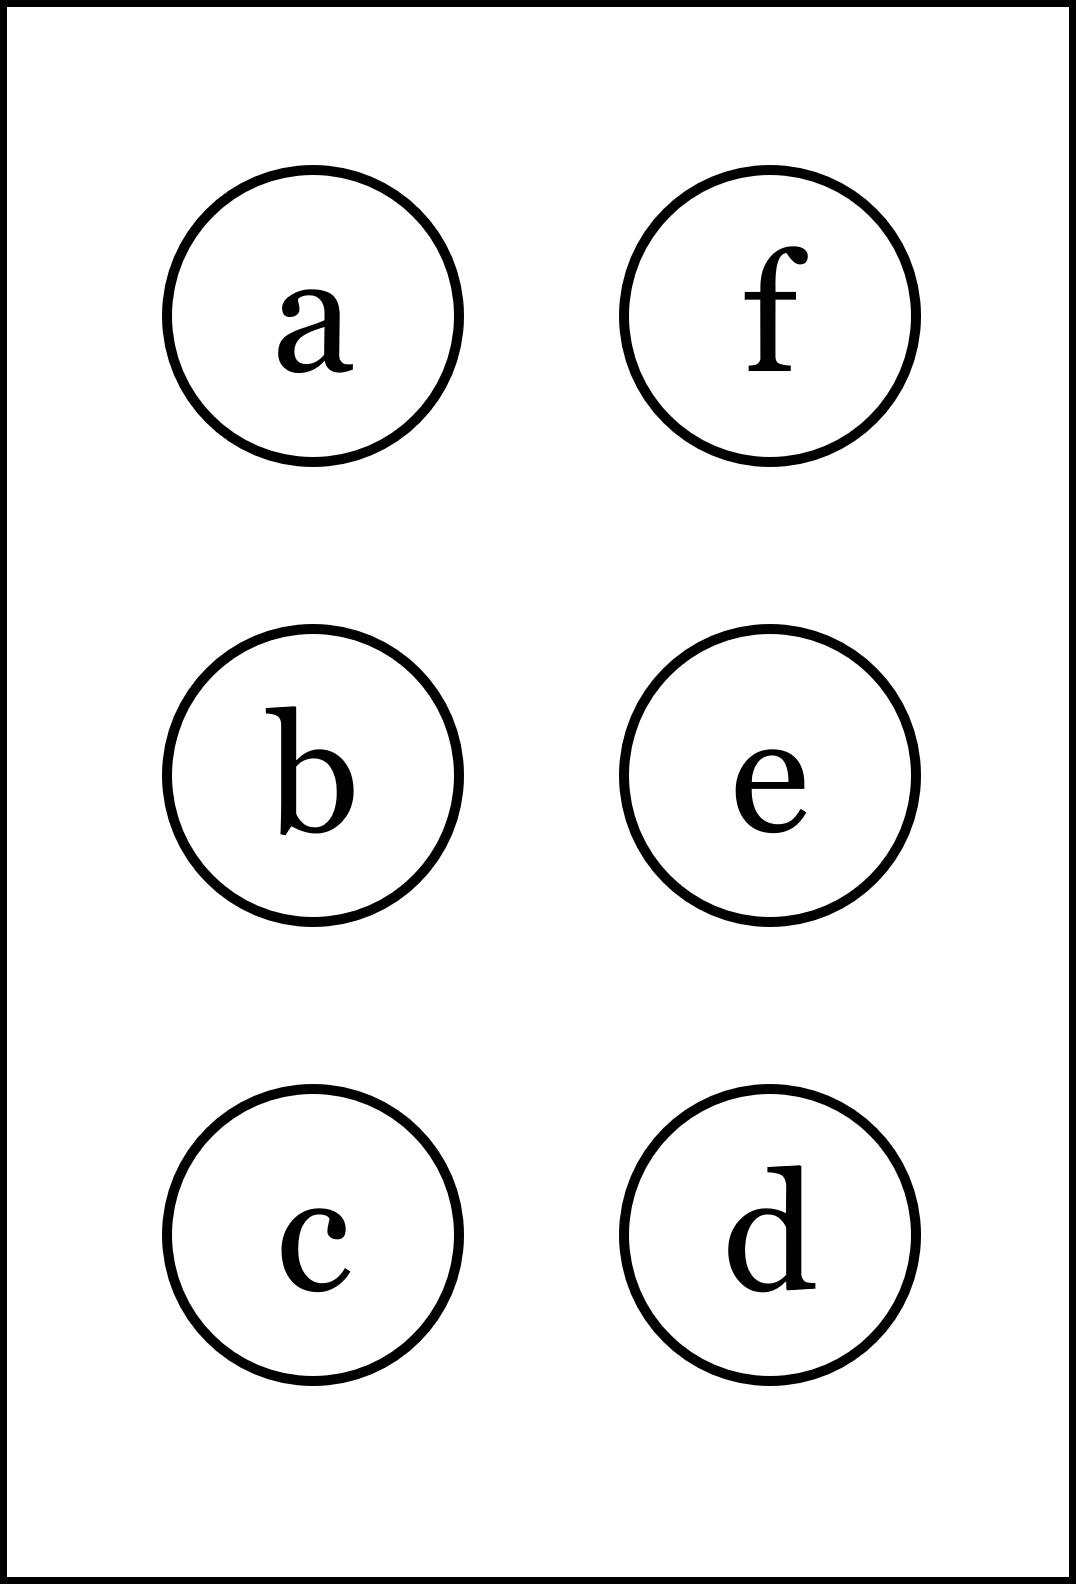
\includegraphics[height=40mm]{../images/braille.png}
{\small Písmeno Braillovej abecedy}
\end{center}
\end{minipage}
\end{center}
\end{minipage}
%
\end{tabular}
\newpage
\thispagestyle{empty}
\begin{tabular}{c:c}
\begin{minipage}[c][104.5mm][t]{0.5\linewidth}
\begin{center}
\vspace{7mm}
{\huge Odmocniny a limity, skupina \textit{Nu $\nu$} -\romannumeral1}\\[5mm]
\textit{Jméno:}\phantom{xxxxxxxxxxxxxxxxxxxxxxxxxxxxxxxxxxxxxxxxxxxxxxxxxxxxxxxxxxxxxxxxx}\\[5mm]
\begin{minipage}{0.95\linewidth}
\begin{center}
V \textbf{(a)} a \textbf{(b)} \textbf{uprav výrazy}, v \textbf{(c)} a \textbf{(d)} \textbf{vypočítaj limity}.\\Pokud se výsledky shodujú s tými za otazníky, tak napravo obarvi\\příslušející kroužek načerno. \textbf{Spolu odevzdejte výsledné slovo}.
\end{center}
\end{minipage}
\\[1mm]
\begin{minipage}{0.79\linewidth}
\begin{center}
\begin{varwidth}{\linewidth}
\begin{enumerate}
\small
\item $\sqrt[1]{\left(\cfrac{x^{4}\;x^{\nicefrac{-3}{2}}}{x^{3}}\right)^{2}}$\quad \dotfill\; ???\;\dotfill \quad $x^{-1}$
\item {\footnotesize{\scriptsize$\big(\sqrt{7x+35y}+\sqrt{7x-35y}\big)^2-\big(\sqrt{7x+35y}-\sqrt{7x-35y}\big)^2$}\quad \dotfill\; ???\;\dotfill \quad $28\sqrt{x^2-25y^2}$}
\item $\lim\limits_{n\to\infty}\cfrac{n^{-1/2}}{\sqrt{36n+5}-\sqrt{36n-3}}$\quad \dotfill\; ???\;\dotfill \quad $\nicefrac{3}{2}$
\item $\lim\limits_{n\to\infty}7n\cfrac{\sqrt{n^2-5n-2}-\sqrt{n^2+5}}{\sqrt{16n^2+8n+7}}$\quad \dotfill\; ???\;\dotfill \quad $\nicefrac{-35}{4}$
\item \quad \dotfill\; ???\;\dotfill \quad vybarvi
\item \quad \dotfill\; ???\;\dotfill \quad nebarvi
\end{enumerate}
\end{varwidth}
\end{center}
\end{minipage}
\begin{minipage}{0.20\linewidth}
\begin{center}
{\Huge\bfseries 1.} \\[2mm]
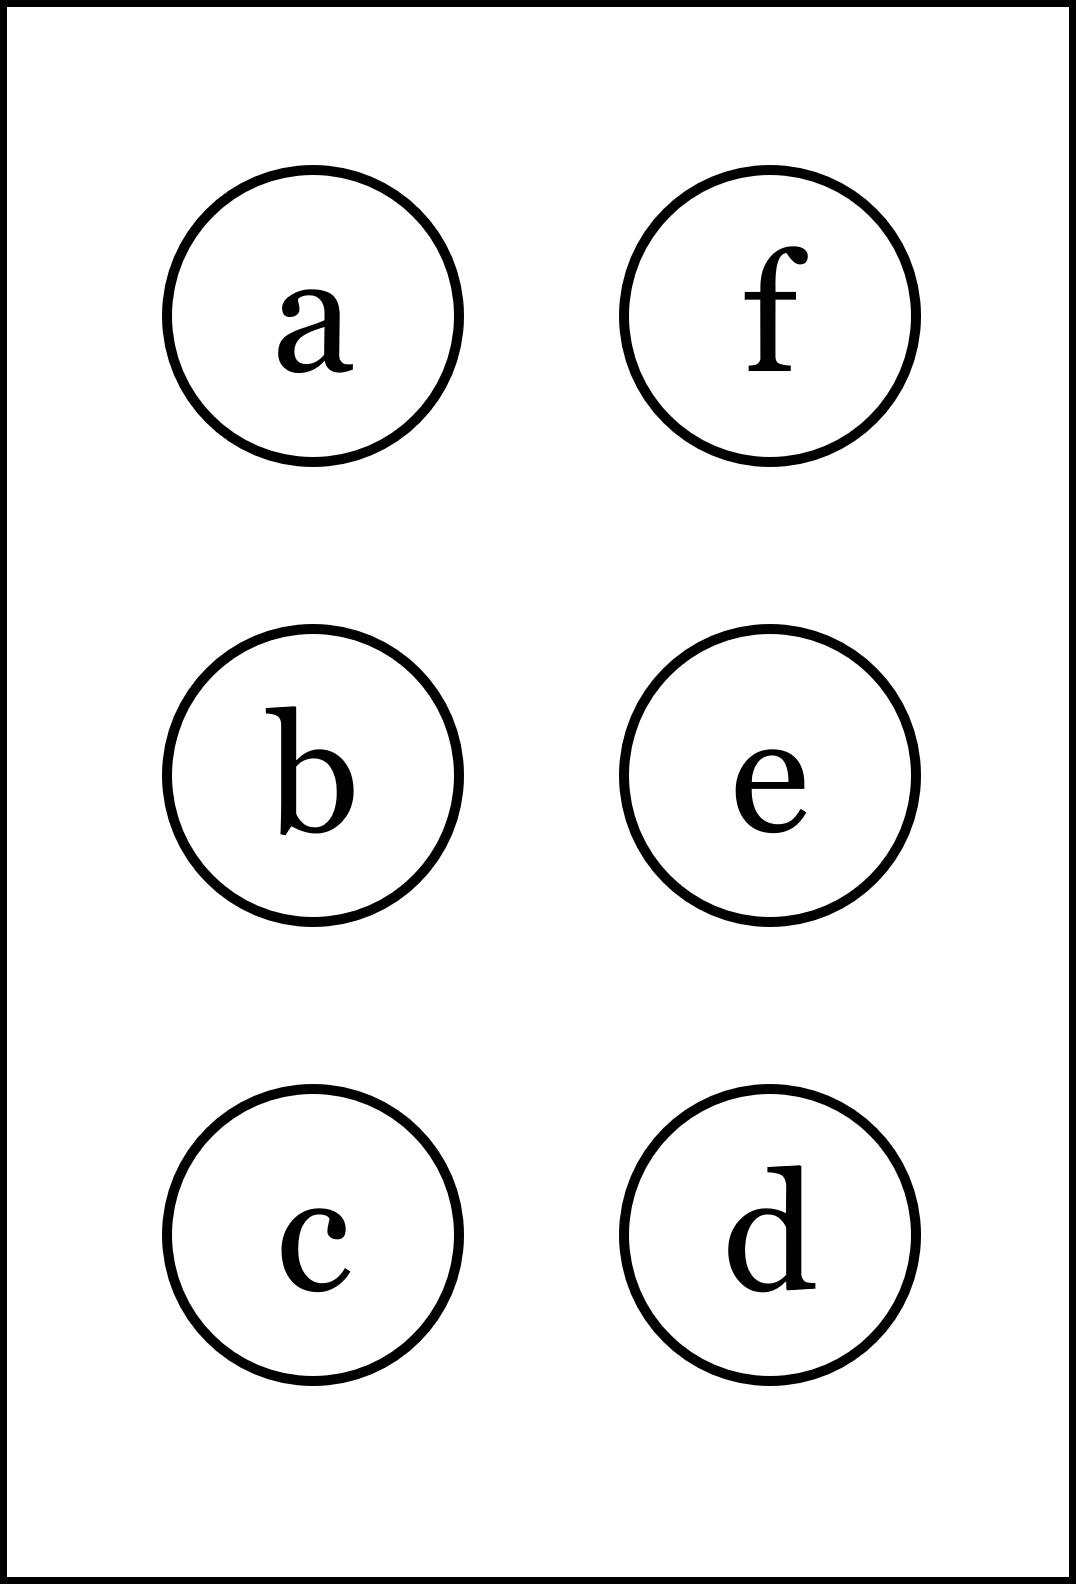
\includegraphics[height=40mm]{../images/braille.png}
{\small Písmeno Braillovej abecedy}
\end{center}
\end{minipage}
\end{center}
\end{minipage}
&
\begin{minipage}[c][104.5mm][t]{0.5\linewidth}
\begin{center}
\vspace{7mm}
{\huge Odmocniny a limity, skupina \textit{Nu $\nu$} -\romannumeral2}\\[5mm]
\textit{Jméno:}\phantom{xxxxxxxxxxxxxxxxxxxxxxxxxxxxxxxxxxxxxxxxxxxxxxxxxxxxxxxxxxxxxxxxx}\\[5mm]
\begin{minipage}{0.95\linewidth}
\begin{center}
V \textbf{(a)} a \textbf{(b)} \textbf{uprav výrazy}, v \textbf{(c)} a \textbf{(d)} \textbf{vypočítaj limity}.\\Pokud se výsledky shodujú s tými za otazníky, tak napravo obarvi\\příslušející kroužek načerno. \textbf{Spolu odevzdejte výsledné slovo}.
\end{center}
\end{minipage}
\\[1mm]
\begin{minipage}{0.79\linewidth}
\begin{center}
\begin{varwidth}{\linewidth}
\begin{enumerate}
\small
\item $\sqrt[1]{\left(\cfrac{x^{1}\;x^{\nicefrac{1}{3}}}{x^{\nicefrac{-1}{4}}}\right)^{4}}$\quad \dotfill\; ???\;\dotfill \quad $x^{\nicefrac{19}{3}}$
\item {\footnotesize{\scriptsize$\big(\sqrt{7x-42y}+\sqrt{7x+42y}\big)^2-\big(\sqrt{7x-42y}-\sqrt{7x+42y}\big)^2$}\quad \dotfill\; ???\;\dotfill \quad $28\sqrt{x^2+6y^2}$}
\item $\lim\limits_{n\to\infty}\cfrac{n^{-1/2}}{\sqrt{36n+6}-\sqrt{36n-7}}$\quad \dotfill\; ???\;\dotfill \quad $\nicefrac{12}{13}$
\item $\lim\limits_{n\to\infty}5n\cfrac{\sqrt{4n^2-7n+4}-\sqrt{4n^2-2}}{\sqrt{16n^2-3n+3}}$\quad \dotfill\; ???\;\dotfill \quad $\nicefrac{-35}{8}$
\item \quad \dotfill\; ???\;\dotfill \quad vybarvi
\item \quad \dotfill\; ???\;\dotfill \quad nebarvi
\end{enumerate}
\end{varwidth}
\end{center}
\end{minipage}
\begin{minipage}{0.20\linewidth}
\begin{center}
{\Huge\bfseries 2.} \\[2mm]
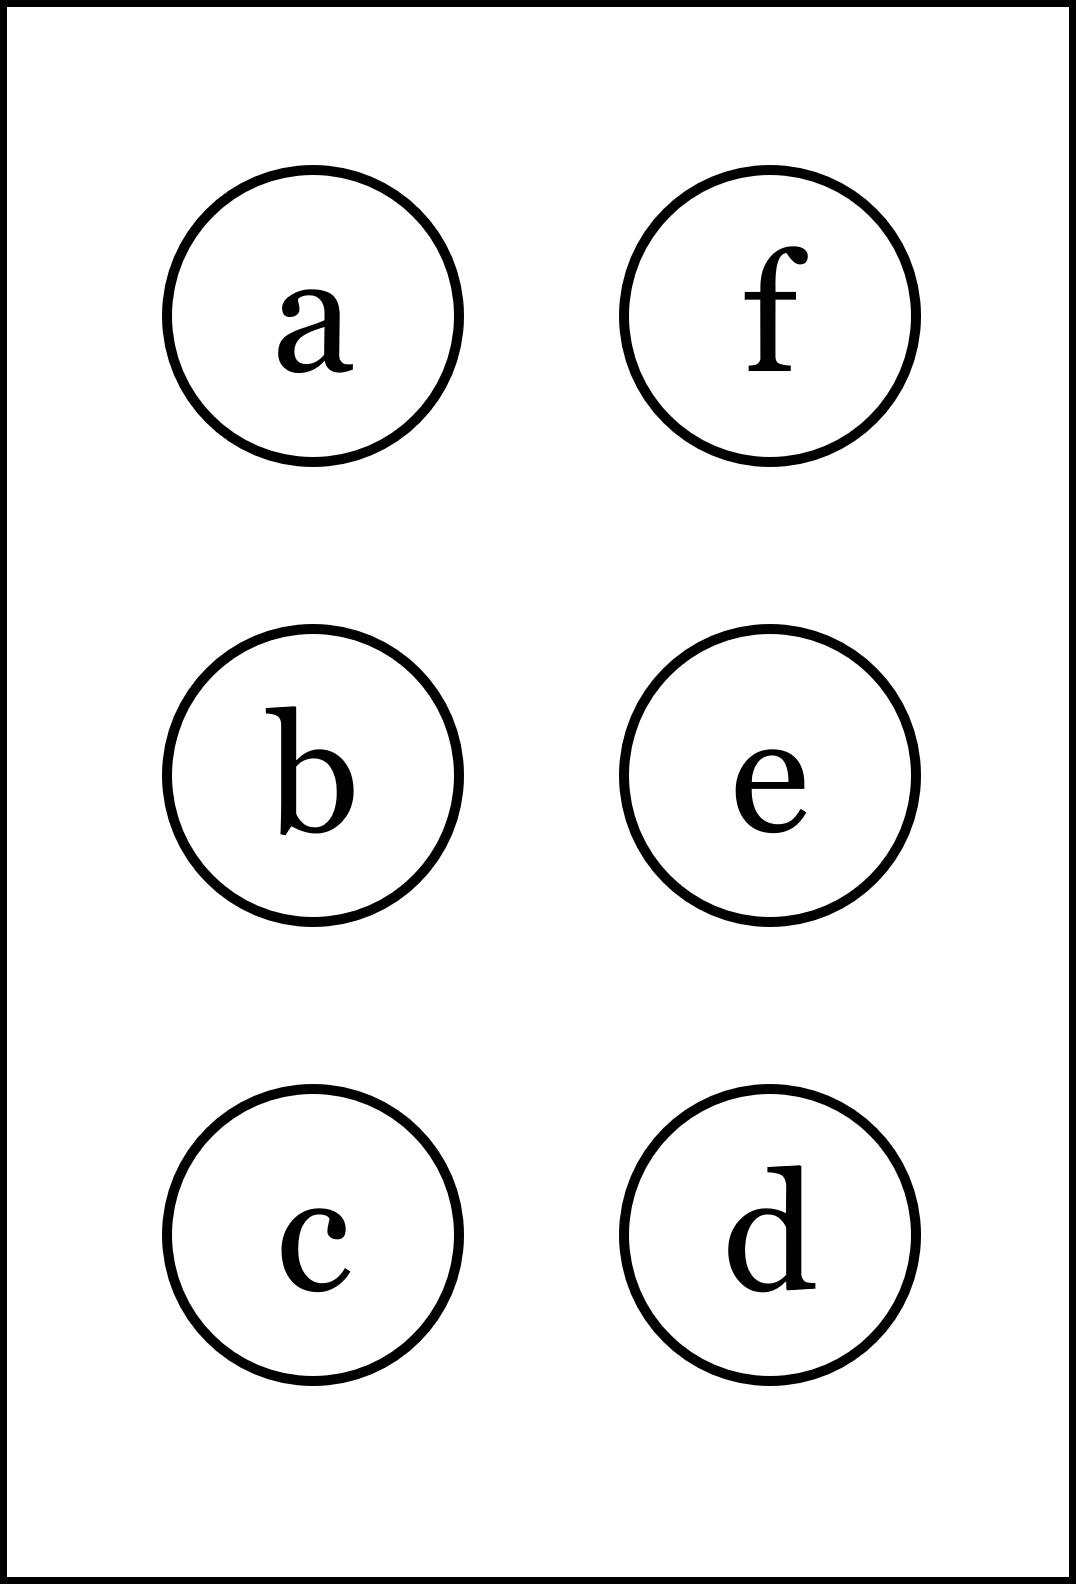
\includegraphics[height=40mm]{../images/braille.png}
{\small Písmeno Braillovej abecedy}
\end{center}
\end{minipage}
\end{center}
\end{minipage}
\\ \hdashline
\begin{minipage}[c][104.5mm][t]{0.5\linewidth}
\begin{center}
\vspace{7mm}
{\huge Odmocniny a limity, skupina \textit{Nu $\nu$} -\romannumeral3}\\[5mm]
\textit{Jméno:}\phantom{xxxxxxxxxxxxxxxxxxxxxxxxxxxxxxxxxxxxxxxxxxxxxxxxxxxxxxxxxxxxxxxxx}\\[5mm]
\begin{minipage}{0.95\linewidth}
\begin{center}
V \textbf{(a)} a \textbf{(b)} \textbf{uprav výrazy}, v \textbf{(c)} a \textbf{(d)} \textbf{vypočítaj limity}.\\Pokud se výsledky shodujú s tými za otazníky, tak napravo obarvi\\příslušející kroužek načerno. \textbf{Spolu odevzdejte výsledné slovo}.
\end{center}
\end{minipage}
\\[1mm]
\begin{minipage}{0.79\linewidth}
\begin{center}
\begin{varwidth}{\linewidth}
\begin{enumerate}
\small
\item $\sqrt[2]{\left(\cfrac{x^{3}\;x^{\nicefrac{1}{6}}}{x^{3}}\right)^{3}}$\quad \dotfill\; ???\;\dotfill \quad $x^{\nicefrac{1}{4}}$
\item {\footnotesize{\scriptsize$\big(\sqrt{x+y}+\sqrt{x-y}\big)^2-\big(\sqrt{x+y}-\sqrt{x-y}\big)^2$}\quad \dotfill\; ???\;\dotfill \quad $4\sqrt{x^2-y^2}$}
\item $\lim\limits_{n\to\infty}\cfrac{n^{-1/2}}{\sqrt{n+2}-\sqrt{n+6}}$\quad \dotfill\; ???\;\dotfill \quad $\nicefrac{-1}{2}$
\item $\lim\limits_{n\to\infty}3n\cfrac{\sqrt{4n^2-2n+3}-\sqrt{4n^2-9}}{\sqrt{9n^2+4n-6}}$\quad \dotfill\; ???\;\dotfill \quad $-1$
\item \quad \dotfill\; ???\;\dotfill \quad nebarvi
\item \quad \dotfill\; ???\;\dotfill \quad vybarvi
\end{enumerate}
\end{varwidth}
\end{center}
\end{minipage}
\begin{minipage}{0.20\linewidth}
\begin{center}
{\Huge\bfseries 3.} \\[2mm]
\includegraphics[height=40mm]{../images/braille.png}
{\small Písmeno Braillovej abecedy}
\end{center}
\end{minipage}
\end{center}
\end{minipage}
&
\begin{minipage}[c][104.5mm][t]{0.5\linewidth}
\begin{center}
\vspace{7mm}
{\huge Odmocniny a limity, skupina \textit{Nu $\nu$} -\romannumeral4}\\[5mm]
\textit{Jméno:}\phantom{xxxxxxxxxxxxxxxxxxxxxxxxxxxxxxxxxxxxxxxxxxxxxxxxxxxxxxxxxxxxxxxxx}\\[5mm]
\begin{minipage}{0.95\linewidth}
\begin{center}
V \textbf{(a)} a \textbf{(b)} \textbf{uprav výrazy}, v \textbf{(c)} a \textbf{(d)} \textbf{vypočítaj limity}.\\Pokud se výsledky shodujú s tými za otazníky, tak napravo obarvi\\příslušející kroužek načerno. \textbf{Spolu odevzdejte výsledné slovo}.
\end{center}
\end{minipage}
\\[1mm]
\begin{minipage}{0.79\linewidth}
\begin{center}
\begin{varwidth}{\linewidth}
\begin{enumerate}
\small
\item $\sqrt[2]{\left(\cfrac{x^{\nicefrac{1}{2}}\;x^{\nicefrac{-1}{3}}}{x^{\nicefrac{-2}{3}}}\right)^{3}}$\quad \dotfill\; ???\;\dotfill \quad $x^{\nicefrac{5}{4}}$
\item {\footnotesize{\scriptsize$\big(\sqrt{2x+10y}+\sqrt{2x-10y}\big)^2-\big(\sqrt{2x+10y}-\sqrt{2x-10y}\big)^2$}\quad \dotfill\; ???\;\dotfill \quad $8\sqrt{x^2-5y^2}$}
\item $\lim\limits_{n\to\infty}\cfrac{n^{-1/2}}{\sqrt{25n+2}-\sqrt{25n-1}}$\quad \dotfill\; ???\;\dotfill \quad $0$
\item $\lim\limits_{n\to\infty}6n\cfrac{\sqrt{9n^2+3n+1}-\sqrt{9n^2-1}}{\sqrt{16n^2-n+2}}$\quad \dotfill\; ???\;\dotfill \quad $\nicefrac{3}{2}$
\item \quad \dotfill\; ???\;\dotfill \quad nebarvi
\item \quad \dotfill\; ???\;\dotfill \quad nebarvi
\end{enumerate}
\end{varwidth}
\end{center}
\end{minipage}
\begin{minipage}{0.20\linewidth}
\begin{center}
{\Huge\bfseries 4.} \\[2mm]
\includegraphics[height=40mm]{../images/braille.png}
{\small Písmeno Braillovej abecedy}
\end{center}
\end{minipage}
\end{center}
\end{minipage}
%
\end{tabular}
\newpage
\thispagestyle{empty}
\begin{tabular}{c:c}
\begin{minipage}[c][104.5mm][t]{0.5\linewidth}
\begin{center}
\vspace{7mm}
{\huge Odmocniny a limity, skupina \textit{Xi $\xi$} -\romannumeral1}\\[5mm]
\textit{Jméno:}\phantom{xxxxxxxxxxxxxxxxxxxxxxxxxxxxxxxxxxxxxxxxxxxxxxxxxxxxxxxxxxxxxxxxx}\\[5mm]
\begin{minipage}{0.95\linewidth}
\begin{center}
V \textbf{(a)} a \textbf{(b)} \textbf{uprav výrazy}, v \textbf{(c)} a \textbf{(d)} \textbf{vypočítaj limity}.\\Pokud se výsledky shodujú s tými za otazníky, tak napravo obarvi\\příslušející kroužek načerno. \textbf{Spolu odevzdejte výsledné slovo}.
\end{center}
\end{minipage}
\\[1mm]
\begin{minipage}{0.79\linewidth}
\begin{center}
\begin{varwidth}{\linewidth}
\begin{enumerate}
\small
\item $\sqrt[9]{\left(\cfrac{x^{\nicefrac{-4}{3}}\;x^{1}}{x^{-1}}\right)^{4}}$\quad \dotfill\; ???\;\dotfill \quad $x^{\nicefrac{8}{27}}$
\item {\footnotesize{\scriptsize$\big(\sqrt{4x-8y}+\sqrt{4x+8y}\big)^2-\big(\sqrt{4x-8y}-\sqrt{4x+8y}\big)^2$}\quad \dotfill\; ???\;\dotfill \quad $16\sqrt{x^2+2y^2}$}
\item $\lim\limits_{n\to\infty}\cfrac{n^{-1/2}}{\sqrt{49n+7}-\sqrt{49n-3}}$\quad \dotfill\; ???\;\dotfill \quad $\nicefrac{7}{5}$
\item $\lim\limits_{n\to\infty}6n\cfrac{\sqrt{49n^2-n-4}-\sqrt{49n^2-4}}{\sqrt{81n^2+n+2}}$\quad \dotfill\; ???\;\dotfill \quad $\nicefrac{-2}{21}$
\item \quad \dotfill\; ???\;\dotfill \quad nebarvi
\item \quad \dotfill\; ???\;\dotfill \quad nebarvi
\end{enumerate}
\end{varwidth}
\end{center}
\end{minipage}
\begin{minipage}{0.20\linewidth}
\begin{center}
{\Huge\bfseries 1.} \\[2mm]
\includegraphics[height=40mm]{../images/braille.png}
{\small Písmeno Braillovej abecedy}
\end{center}
\end{minipage}
\end{center}
\end{minipage}
&
\begin{minipage}[c][104.5mm][t]{0.5\linewidth}
\begin{center}
\vspace{7mm}
{\huge Odmocniny a limity, skupina \textit{Xi $\xi$} -\romannumeral2}\\[5mm]
\textit{Jméno:}\phantom{xxxxxxxxxxxxxxxxxxxxxxxxxxxxxxxxxxxxxxxxxxxxxxxxxxxxxxxxxxxxxxxxx}\\[5mm]
\begin{minipage}{0.95\linewidth}
\begin{center}
V \textbf{(a)} a \textbf{(b)} \textbf{uprav výrazy}, v \textbf{(c)} a \textbf{(d)} \textbf{vypočítaj limity}.\\Pokud se výsledky shodujú s tými za otazníky, tak napravo obarvi\\příslušející kroužek načerno. \textbf{Spolu odevzdejte výsledné slovo}.
\end{center}
\end{minipage}
\\[1mm]
\begin{minipage}{0.79\linewidth}
\begin{center}
\begin{varwidth}{\linewidth}
\begin{enumerate}
\small
\item $\sqrt[1]{\left(\cfrac{x^{\nicefrac{-5}{4}}\;x^{1}}{x^{\nicefrac{5}{2}}}\right)^{2}}$\quad \dotfill\; ???\;\dotfill \quad $x^{\nicefrac{-11}{2}}$
\item {\footnotesize{\scriptsize$\big(\sqrt{3x-21y}+\sqrt{3x+21y}\big)^2-\big(\sqrt{3x-21y}-\sqrt{3x+21y}\big)^2$}\quad \dotfill\; ???\;\dotfill \quad $12\sqrt{x^2+7y^2}$}
\item $\lim\limits_{n\to\infty}\cfrac{n^{-1/2}}{\sqrt{49n+3}-\sqrt{49n-9}}$\quad \dotfill\; ???\;\dotfill \quad $\nicefrac{7}{6}$
\item $\lim\limits_{n\to\infty}8n\cfrac{\sqrt{25n^2-2n-4}-\sqrt{25n^2-1}}{\sqrt{9n^2+4n+3}}$\quad \dotfill\; ???\;\dotfill \quad $\nicefrac{-16}{15}$
\item \quad \dotfill\; ???\;\dotfill \quad vybarvi
\item \quad \dotfill\; ???\;\dotfill \quad nebarvi
\end{enumerate}
\end{varwidth}
\end{center}
\end{minipage}
\begin{minipage}{0.20\linewidth}
\begin{center}
{\Huge\bfseries 2.} \\[2mm]
\includegraphics[height=40mm]{../images/braille.png}
{\small Písmeno Braillovej abecedy}
\end{center}
\end{minipage}
\end{center}
\end{minipage}
\\ \hdashline
\begin{minipage}[c][104.5mm][t]{0.5\linewidth}
\begin{center}
\vspace{7mm}
{\huge Odmocniny a limity, skupina \textit{Xi $\xi$} -\romannumeral3}\\[5mm]
\textit{Jméno:}\phantom{xxxxxxxxxxxxxxxxxxxxxxxxxxxxxxxxxxxxxxxxxxxxxxxxxxxxxxxxxxxxxxxxx}\\[5mm]
\begin{minipage}{0.95\linewidth}
\begin{center}
V \textbf{(a)} a \textbf{(b)} \textbf{uprav výrazy}, v \textbf{(c)} a \textbf{(d)} \textbf{vypočítaj limity}.\\Pokud se výsledky shodujú s tými za otazníky, tak napravo obarvi\\příslušející kroužek načerno. \textbf{Spolu odevzdejte výsledné slovo}.
\end{center}
\end{minipage}
\\[1mm]
\begin{minipage}{0.79\linewidth}
\begin{center}
\begin{varwidth}{\linewidth}
\begin{enumerate}
\small
\item $\sqrt[1]{\left(\cfrac{x^{-1}\;x^{\nicefrac{2}{3}}}{x^{\nicefrac{2}{3}}}\right)^{7}}$\quad \dotfill\; ???\;\dotfill \quad $x^{\nicefrac{-49}{3}}$
\item {\footnotesize{\scriptsize$\big(\sqrt{x-9y}+\sqrt{x+9y}\big)^2-\big(\sqrt{x-9y}-\sqrt{x+9y}\big)^2$}\quad \dotfill\; ???\;\dotfill \quad $4\sqrt{x^2-81y^2}$}
\item $\lim\limits_{n\to\infty}\cfrac{n^{-1/2}}{\sqrt{n+9}-\sqrt{n-6}}$\quad \dotfill\; ???\;\dotfill \quad $\nicefrac{2}{15}$
\item $\lim\limits_{n\to\infty}3n\cfrac{\sqrt{36n^2+7n+2}-\sqrt{36n^2-1}}{\sqrt{16n^2-3n-3}}$\quad \dotfill\; ???\;\dotfill \quad $\nicefrac{7}{8}$
\item \quad \dotfill\; ???\;\dotfill \quad nebarvi
\item \quad \dotfill\; ???\;\dotfill \quad vybarvi
\end{enumerate}
\end{varwidth}
\end{center}
\end{minipage}
\begin{minipage}{0.20\linewidth}
\begin{center}
{\Huge\bfseries 3.} \\[2mm]
\includegraphics[height=40mm]{../images/braille.png}
{\small Písmeno Braillovej abecedy}
\end{center}
\end{minipage}
\end{center}
\end{minipage}
&
\begin{minipage}[c][104.5mm][t]{0.5\linewidth}
\begin{center}
\vspace{7mm}
{\huge Odmocniny a limity, skupina \textit{Xi $\xi$} -\romannumeral4}\\[5mm]
\textit{Jméno:}\phantom{xxxxxxxxxxxxxxxxxxxxxxxxxxxxxxxxxxxxxxxxxxxxxxxxxxxxxxxxxxxxxxxxx}\\[5mm]
\begin{minipage}{0.95\linewidth}
\begin{center}
V \textbf{(a)} a \textbf{(b)} \textbf{uprav výrazy}, v \textbf{(c)} a \textbf{(d)} \textbf{vypočítaj limity}.\\Pokud se výsledky shodujú s tými za otazníky, tak napravo obarvi\\příslušející kroužek načerno. \textbf{Spolu odevzdejte výsledné slovo}.
\end{center}
\end{minipage}
\\[1mm]
\begin{minipage}{0.79\linewidth}
\begin{center}
\begin{varwidth}{\linewidth}
\begin{enumerate}
\small
\item $\sqrt[6]{\left(\cfrac{x^{-1}\;x^{1}}{x^{\nicefrac{-3}{7}}}\right)^{7}}$\quad \dotfill\; ???\;\dotfill \quad $x^{\nicefrac{-11}{6}}$
\item {\footnotesize{\scriptsize$\big(\sqrt{x-3y}+\sqrt{x+3y}\big)^2-\big(\sqrt{x-3y}-\sqrt{x+3y}\big)^2$}\quad \dotfill\; ???\;\dotfill \quad $4\sqrt{x^2-9y^2}$}
\item $\lim\limits_{n\to\infty}\cfrac{n^{-1/2}}{\sqrt{49n-5}-\sqrt{49n+1}}$\quad \dotfill\; ???\;\dotfill \quad $\nicefrac{-7}{3}$
\item $\lim\limits_{n\to\infty}3n\cfrac{\sqrt{49n^2+n-3}-\sqrt{49n^2+1}}{\sqrt{9n^2+9n+1}}$\quad \dotfill\; ???\;\dotfill \quad $\nicefrac{1}{7}$
\item \quad \dotfill\; ???\;\dotfill \quad vybarvi
\item \quad \dotfill\; ???\;\dotfill \quad vybarvi
\end{enumerate}
\end{varwidth}
\end{center}
\end{minipage}
\begin{minipage}{0.20\linewidth}
\begin{center}
{\Huge\bfseries 4.} \\[2mm]
\includegraphics[height=40mm]{../images/braille.png}
{\small Písmeno Braillovej abecedy}
\end{center}
\end{minipage}
\end{center}
\end{minipage}
%
\end{tabular}
\newpage
\thispagestyle{empty}
\begin{tabular}{c:c}
\begin{minipage}[c][104.5mm][t]{0.5\linewidth}
\begin{center}
\vspace{7mm}
{\huge Odmocniny a limity, skupina \textit{Omicron $\omicron$} -\romannumeral1}\\[5mm]
\textit{Jméno:}\phantom{xxxxxxxxxxxxxxxxxxxxxxxxxxxxxxxxxxxxxxxxxxxxxxxxxxxxxxxxxxxxxxxxx}\\[5mm]
\begin{minipage}{0.95\linewidth}
\begin{center}
V \textbf{(a)} a \textbf{(b)} \textbf{uprav výrazy}, v \textbf{(c)} a \textbf{(d)} \textbf{vypočítaj limity}.\\Pokud se výsledky shodujú s tými za otazníky, tak napravo obarvi\\příslušející kroužek načerno. \textbf{Spolu odevzdejte výsledné slovo}.
\end{center}
\end{minipage}
\\[1mm]
\begin{minipage}{0.79\linewidth}
\begin{center}
\begin{varwidth}{\linewidth}
\begin{enumerate}
\small
\item $\sqrt[2]{\left(\cfrac{x^{1}\;x^{-6}}{x^{3}}\right)^{4}}$\quad \dotfill\; ???\;\dotfill \quad $x^{-16}$
\item {\footnotesize{\scriptsize$\big(\sqrt{3x+6y}+\sqrt{3x-6y}\big)^2-\big(\sqrt{3x+6y}-\sqrt{3x-6y}\big)^2$}\quad \dotfill\; ???\;\dotfill \quad $12\sqrt{x^2-2y^2}$}
\item $\lim\limits_{n\to\infty}\cfrac{n^{-1/2}}{\sqrt{16n+9}-\sqrt{16n-2}}$\quad \dotfill\; ???\;\dotfill \quad $\nicefrac{8}{11}$
\item $\lim\limits_{n\to\infty}3n\cfrac{\sqrt{25n^2+n-7}-\sqrt{25n^2-4}}{\sqrt{4n^2-3n+6}}$\quad \dotfill\; ???\;\dotfill \quad $\nicefrac{3}{10}$
\item \quad \dotfill\; ???\;\dotfill \quad nebarvi
\item \quad \dotfill\; ???\;\dotfill \quad nebarvi
\end{enumerate}
\end{varwidth}
\end{center}
\end{minipage}
\begin{minipage}{0.20\linewidth}
\begin{center}
{\Huge\bfseries 1.} \\[2mm]
\includegraphics[height=40mm]{../images/braille.png}
{\small Písmeno Braillovej abecedy}
\end{center}
\end{minipage}
\end{center}
\end{minipage}
&
\begin{minipage}[c][104.5mm][t]{0.5\linewidth}
\begin{center}
\vspace{7mm}
{\huge Odmocniny a limity, skupina \textit{Omicron $\omicron$} -\romannumeral2}\\[5mm]
\textit{Jméno:}\phantom{xxxxxxxxxxxxxxxxxxxxxxxxxxxxxxxxxxxxxxxxxxxxxxxxxxxxxxxxxxxxxxxxx}\\[5mm]
\begin{minipage}{0.95\linewidth}
\begin{center}
V \textbf{(a)} a \textbf{(b)} \textbf{uprav výrazy}, v \textbf{(c)} a \textbf{(d)} \textbf{vypočítaj limity}.\\Pokud se výsledky shodujú s tými za otazníky, tak napravo obarvi\\příslušející kroužek načerno. \textbf{Spolu odevzdejte výsledné slovo}.
\end{center}
\end{minipage}
\\[1mm]
\begin{minipage}{0.79\linewidth}
\begin{center}
\begin{varwidth}{\linewidth}
\begin{enumerate}
\small
\item $\sqrt[6]{\left(\cfrac{x^{-4}\;x^{-1}}{x^{7}}\right)^{2}}$\quad \dotfill\; ???\;\dotfill \quad $x^{-4}$
\item {\footnotesize{\scriptsize$\big(\sqrt{4x+8y}+\sqrt{4x-8y}\big)^2-\big(\sqrt{4x+8y}-\sqrt{4x-8y}\big)^2$}\quad \dotfill\; ???\;\dotfill \quad $16\sqrt{x^2-2y^2}$}
\item $\lim\limits_{n\to\infty}\cfrac{n^{-1/2}}{\sqrt{64n+1}-\sqrt{64n+3}}$\quad \dotfill\; ???\;\dotfill \quad $-8$
\item $\lim\limits_{n\to\infty}5n\cfrac{\sqrt{25n^2-3n-5}-\sqrt{25n^2-5}}{\sqrt{16n^2-4n+5}}$\quad \dotfill\; ???\;\dotfill \quad $\nicefrac{-3}{4}$
\item \quad \dotfill\; ???\;\dotfill \quad vybarvi
\item \quad \dotfill\; ???\;\dotfill \quad nebarvi
\end{enumerate}
\end{varwidth}
\end{center}
\end{minipage}
\begin{minipage}{0.20\linewidth}
\begin{center}
{\Huge\bfseries 2.} \\[2mm]
\includegraphics[height=40mm]{../images/braille.png}
{\small Písmeno Braillovej abecedy}
\end{center}
\end{minipage}
\end{center}
\end{minipage}
\\ \hdashline
\begin{minipage}[c][104.5mm][t]{0.5\linewidth}
\begin{center}
\vspace{7mm}
{\huge Odmocniny a limity, skupina \textit{Omicron $\omicron$} -\romannumeral3}\\[5mm]
\textit{Jméno:}\phantom{xxxxxxxxxxxxxxxxxxxxxxxxxxxxxxxxxxxxxxxxxxxxxxxxxxxxxxxxxxxxxxxxx}\\[5mm]
\begin{minipage}{0.95\linewidth}
\begin{center}
V \textbf{(a)} a \textbf{(b)} \textbf{uprav výrazy}, v \textbf{(c)} a \textbf{(d)} \textbf{vypočítaj limity}.\\Pokud se výsledky shodujú s tými za otazníky, tak napravo obarvi\\příslušející kroužek načerno. \textbf{Spolu odevzdejte výsledné slovo}.
\end{center}
\end{minipage}
\\[1mm]
\begin{minipage}{0.79\linewidth}
\begin{center}
\begin{varwidth}{\linewidth}
\begin{enumerate}
\small
\item $\sqrt[1]{\left(\cfrac{x^{-1}\;x^{-3}}{x^{-6}}\right)^{3}}$\quad \dotfill\; ???\;\dotfill \quad $x^{6}$
\item {\footnotesize{\scriptsize$\big(\sqrt{6x-30y}+\sqrt{6x+30y}\big)^2-\big(\sqrt{6x-30y}-\sqrt{6x+30y}\big)^2$}\quad \dotfill\; ???\;\dotfill \quad $24\sqrt{x^2-25y^2}$}
\item $\lim\limits_{n\to\infty}\cfrac{n^{-1/2}}{\sqrt{4n-5}-\sqrt{4n+6}}$\quad \dotfill\; ???\;\dotfill \quad $\nicefrac{-4}{11}$
\item $\lim\limits_{n\to\infty}7n\cfrac{\sqrt{25n^2-5n+3}-\sqrt{25n^2+7}}{\sqrt{9n^2+7n+8}}$\quad \dotfill\; ???\;\dotfill \quad $\nicefrac{-7}{3}$
\item \quad \dotfill\; ???\;\dotfill \quad nebarvi
\item \quad \dotfill\; ???\;\dotfill \quad nebarvi
\end{enumerate}
\end{varwidth}
\end{center}
\end{minipage}
\begin{minipage}{0.20\linewidth}
\begin{center}
{\Huge\bfseries 3.} \\[2mm]
\includegraphics[height=40mm]{../images/braille.png}
{\small Písmeno Braillovej abecedy}
\end{center}
\end{minipage}
\end{center}
\end{minipage}
&
\begin{minipage}[c][104.5mm][t]{0.5\linewidth}
\begin{center}
\vspace{7mm}
{\huge Odmocniny a limity, skupina \textit{Omicron $\omicron$} -\romannumeral4}\\[5mm]
\textit{Jméno:}\phantom{xxxxxxxxxxxxxxxxxxxxxxxxxxxxxxxxxxxxxxxxxxxxxxxxxxxxxxxxxxxxxxxxx}\\[5mm]
\begin{minipage}{0.95\linewidth}
\begin{center}
V \textbf{(a)} a \textbf{(b)} \textbf{uprav výrazy}, v \textbf{(c)} a \textbf{(d)} \textbf{vypočítaj limity}.\\Pokud se výsledky shodujú s tými za otazníky, tak napravo obarvi\\příslušející kroužek načerno. \textbf{Spolu odevzdejte výsledné slovo}.
\end{center}
\end{minipage}
\\[1mm]
\begin{minipage}{0.79\linewidth}
\begin{center}
\begin{varwidth}{\linewidth}
\begin{enumerate}
\small
\item $\sqrt[5]{\left(\cfrac{x^{1}\;x^{4}}{x^{6}}\right)^{5}}$\quad \dotfill\; ???\;\dotfill \quad $x^{-1}$
\item {\footnotesize{\scriptsize$\big(\sqrt{6x-12y}+\sqrt{6x+12y}\big)^2-\big(\sqrt{6x-12y}-\sqrt{6x+12y}\big)^2$}\quad \dotfill\; ???\;\dotfill \quad $24\sqrt{x^2+2y^2}$}
\item $\lim\limits_{n\to\infty}\cfrac{n^{-1/2}}{\sqrt{4n-5}-\sqrt{4n+6}}$\quad \dotfill\; ???\;\dotfill \quad $\nicefrac{-4}{11}$
\item $\lim\limits_{n\to\infty}5n\cfrac{\sqrt{25n^2-2n-1}-\sqrt{25n^2-2}}{\sqrt{4n^2+2n-4}}$\quad \dotfill\; ???\;\dotfill \quad $-1$
\item \quad \dotfill\; ???\;\dotfill \quad vybarvi
\item \quad \dotfill\; ???\;\dotfill \quad nebarvi
\end{enumerate}
\end{varwidth}
\end{center}
\end{minipage}
\begin{minipage}{0.20\linewidth}
\begin{center}
{\Huge\bfseries 4.} \\[2mm]
\includegraphics[height=40mm]{../images/braille.png}
{\small Písmeno Braillovej abecedy}
\end{center}
\end{minipage}
\end{center}
\end{minipage}
%
\end{tabular}
\newpage
\thispagestyle{empty}
\begin{tabular}{c:c}
\begin{minipage}[c][104.5mm][t]{0.5\linewidth}
\begin{center}
\vspace{7mm}
{\huge Odmocniny a limity, skupina \textit{Pi $\pi$} -\romannumeral1}\\[5mm]
\textit{Jméno:}\phantom{xxxxxxxxxxxxxxxxxxxxxxxxxxxxxxxxxxxxxxxxxxxxxxxxxxxxxxxxxxxxxxxxx}\\[5mm]
\begin{minipage}{0.95\linewidth}
\begin{center}
V \textbf{(a)} a \textbf{(b)} \textbf{uprav výrazy}, v \textbf{(c)} a \textbf{(d)} \textbf{vypočítaj limity}.\\Pokud se výsledky shodujú s tými za otazníky, tak napravo obarvi\\příslušející kroužek načerno. \textbf{Spolu odevzdejte výsledné slovo}.
\end{center}
\end{minipage}
\\[1mm]
\begin{minipage}{0.79\linewidth}
\begin{center}
\begin{varwidth}{\linewidth}
\begin{enumerate}
\small
\item $\sqrt[6]{\left(\cfrac{x^{\nicefrac{-2}{3}}\;x^{5}}{x^{-4}}\right)^{5}}$\quad \dotfill\; ???\;\dotfill \quad $x^{\nicefrac{125}{18}}$
\item {\footnotesize{\scriptsize$\big(\sqrt{2x+14y}+\sqrt{2x-14y}\big)^2-\big(\sqrt{2x+14y}-\sqrt{2x-14y}\big)^2$}\quad \dotfill\; ???\;\dotfill \quad $8\sqrt{x^2-7y^2}$}
\item $\lim\limits_{n\to\infty}\cfrac{n^{-1/2}}{\sqrt{25n-3}-\sqrt{25n-1}}$\quad \dotfill\; ???\;\dotfill \quad $\nicefrac{-5}{2}$
\item $\lim\limits_{n\to\infty}7n\cfrac{\sqrt{9n^2-8n-4}-\sqrt{9n^2-5}}{\sqrt{4n^2-8n-5}}$\quad \dotfill\; ???\;\dotfill \quad $\nicefrac{-14}{3}$
\item \quad \dotfill\; ???\;\dotfill \quad nebarvi
\item \quad \dotfill\; ???\;\dotfill \quad vybarvi
\end{enumerate}
\end{varwidth}
\end{center}
\end{minipage}
\begin{minipage}{0.20\linewidth}
\begin{center}
{\Huge\bfseries 1.} \\[2mm]
\includegraphics[height=40mm]{../images/braille.png}
{\small Písmeno Braillovej abecedy}
\end{center}
\end{minipage}
\end{center}
\end{minipage}
&
\begin{minipage}[c][104.5mm][t]{0.5\linewidth}
\begin{center}
\vspace{7mm}
{\huge Odmocniny a limity, skupina \textit{Pi $\pi$} -\romannumeral2}\\[5mm]
\textit{Jméno:}\phantom{xxxxxxxxxxxxxxxxxxxxxxxxxxxxxxxxxxxxxxxxxxxxxxxxxxxxxxxxxxxxxxxxx}\\[5mm]
\begin{minipage}{0.95\linewidth}
\begin{center}
V \textbf{(a)} a \textbf{(b)} \textbf{uprav výrazy}, v \textbf{(c)} a \textbf{(d)} \textbf{vypočítaj limity}.\\Pokud se výsledky shodujú s tými za otazníky, tak napravo obarvi\\příslušející kroužek načerno. \textbf{Spolu odevzdejte výsledné slovo}.
\end{center}
\end{minipage}
\\[1mm]
\begin{minipage}{0.79\linewidth}
\begin{center}
\begin{varwidth}{\linewidth}
\begin{enumerate}
\small
\item $\sqrt[7]{\left(\cfrac{x^{-1}\;x^{\nicefrac{-5}{3}}}{x^{\nicefrac{-1}{2}}}\right)^{3}}$\quad \dotfill\; ???\;\dotfill \quad $x^{\nicefrac{-13}{14}}$
\item {\footnotesize{\scriptsize$\big(\sqrt{8x+8y}+\sqrt{8x-8y}\big)^2-\big(\sqrt{8x+8y}-\sqrt{8x-8y}\big)^2$}\quad \dotfill\; ???\;\dotfill \quad $16\sqrt{x^2-y^2}$}
\item $\lim\limits_{n\to\infty}\cfrac{n^{-1/2}}{\sqrt{64n-2}-\sqrt{64n-5}}$\quad \dotfill\; ???\;\dotfill \quad $\nicefrac{16}{3}$
\item $\lim\limits_{n\to\infty}4n\cfrac{\sqrt{64n^2+3n-1}-\sqrt{64n^2-6}}{\sqrt{4n^2+3n+1}}$\quad \dotfill\; ???\;\dotfill \quad $\nicefrac{3}{4}$
\item \quad \dotfill\; ???\;\dotfill \quad vybarvi
\item \quad \dotfill\; ???\;\dotfill \quad nebarvi
\end{enumerate}
\end{varwidth}
\end{center}
\end{minipage}
\begin{minipage}{0.20\linewidth}
\begin{center}
{\Huge\bfseries 2.} \\[2mm]
\includegraphics[height=40mm]{../images/braille.png}
{\small Písmeno Braillovej abecedy}
\end{center}
\end{minipage}
\end{center}
\end{minipage}
\\ \hdashline
\begin{minipage}[c][104.5mm][t]{0.5\linewidth}
\begin{center}
\vspace{7mm}
{\huge Odmocniny a limity, skupina \textit{Pi $\pi$} -\romannumeral3}\\[5mm]
\textit{Jméno:}\phantom{xxxxxxxxxxxxxxxxxxxxxxxxxxxxxxxxxxxxxxxxxxxxxxxxxxxxxxxxxxxxxxxxx}\\[5mm]
\begin{minipage}{0.95\linewidth}
\begin{center}
V \textbf{(a)} a \textbf{(b)} \textbf{uprav výrazy}, v \textbf{(c)} a \textbf{(d)} \textbf{vypočítaj limity}.\\Pokud se výsledky shodujú s tými za otazníky, tak napravo obarvi\\příslušející kroužek načerno. \textbf{Spolu odevzdejte výsledné slovo}.
\end{center}
\end{minipage}
\\[1mm]
\begin{minipage}{0.79\linewidth}
\begin{center}
\begin{varwidth}{\linewidth}
\begin{enumerate}
\small
\item $\sqrt[1]{\left(\cfrac{x^{4}\;x^{\nicefrac{1}{3}}}{x^{7}}\right)^{2}}$\quad \dotfill\; ???\;\dotfill \quad $x^{\nicefrac{-16}{3}}$
\item {\footnotesize{\scriptsize$\big(\sqrt{5x-20y}+\sqrt{5x+20y}\big)^2-\big(\sqrt{5x-20y}-\sqrt{5x+20y}\big)^2$}\quad \dotfill\; ???\;\dotfill \quad $20\sqrt{x^2+4y^2}$}
\item $\lim\limits_{n\to\infty}\cfrac{n^{-1/2}}{\sqrt{n-4}-\sqrt{n+3}}$\quad \dotfill\; ???\;\dotfill \quad $\nicefrac{-2}{7}$
\item $\lim\limits_{n\to\infty}6n\cfrac{\sqrt{n^2+2n+1}-\sqrt{n^2+9}}{\sqrt{36n^2+4n-4}}$\quad \dotfill\; ???\;\dotfill \quad $2$
\item \quad \dotfill\; ???\;\dotfill \quad nebarvi
\item \quad \dotfill\; ???\;\dotfill \quad nebarvi
\end{enumerate}
\end{varwidth}
\end{center}
\end{minipage}
\begin{minipage}{0.20\linewidth}
\begin{center}
{\Huge\bfseries 3.} \\[2mm]
\includegraphics[height=40mm]{../images/braille.png}
{\small Písmeno Braillovej abecedy}
\end{center}
\end{minipage}
\end{center}
\end{minipage}
&
\begin{minipage}[c][104.5mm][t]{0.5\linewidth}
\begin{center}
\vspace{7mm}
{\huge Odmocniny a limity, skupina \textit{Pi $\pi$} -\romannumeral4}\\[5mm]
\textit{Jméno:}\phantom{xxxxxxxxxxxxxxxxxxxxxxxxxxxxxxxxxxxxxxxxxxxxxxxxxxxxxxxxxxxxxxxxx}\\[5mm]
\begin{minipage}{0.95\linewidth}
\begin{center}
V \textbf{(a)} a \textbf{(b)} \textbf{uprav výrazy}, v \textbf{(c)} a \textbf{(d)} \textbf{vypočítaj limity}.\\Pokud se výsledky shodujú s tými za otazníky, tak napravo obarvi\\příslušející kroužek načerno. \textbf{Spolu odevzdejte výsledné slovo}.
\end{center}
\end{minipage}
\\[1mm]
\begin{minipage}{0.79\linewidth}
\begin{center}
\begin{varwidth}{\linewidth}
\begin{enumerate}
\small
\item $\sqrt[3]{\left(\cfrac{x^{1}\;x^{-3}}{x^{\nicefrac{1}{4}}}\right)^{3}}$\quad \dotfill\; ???\;\dotfill \quad $x^{\nicefrac{-9}{4}}$
\item {\footnotesize{\scriptsize$\big(\sqrt{5x+15y}+\sqrt{5x-15y}\big)^2-\big(\sqrt{5x+15y}-\sqrt{5x-15y}\big)^2$}\quad \dotfill\; ???\;\dotfill \quad $20\sqrt{x^2-9y^2}$}
\item $\lim\limits_{n\to\infty}\cfrac{n^{-1/2}}{\sqrt{49n+6}-\sqrt{49n-2}}$\quad \dotfill\; ???\;\dotfill \quad $\nicefrac{7}{4}$
\item $\lim\limits_{n\to\infty}2n\cfrac{\sqrt{n^2-n+1}-\sqrt{n^2+5}}{\sqrt{64n^2+4n-5}}$\quad \dotfill\; ???\;\dotfill \quad $\nicefrac{-1}{4}$
\item \quad \dotfill\; ???\;\dotfill \quad nebarvi
\item \quad \dotfill\; ???\;\dotfill \quad nebarvi
\end{enumerate}
\end{varwidth}
\end{center}
\end{minipage}
\begin{minipage}{0.20\linewidth}
\begin{center}
{\Huge\bfseries 4.} \\[2mm]
\includegraphics[height=40mm]{../images/braille.png}
{\small Písmeno Braillovej abecedy}
\end{center}
\end{minipage}
\end{center}
\end{minipage}
%
\end{tabular}
\newpage
\thispagestyle{empty}
\begin{tabular}{c:c}
\begin{minipage}[c][104.5mm][t]{0.5\linewidth}
\begin{center}
\vspace{7mm}
{\huge Odmocniny a limity, skupina \textit{Rho $\rho$} -\romannumeral1}\\[5mm]
\textit{Jméno:}\phantom{xxxxxxxxxxxxxxxxxxxxxxxxxxxxxxxxxxxxxxxxxxxxxxxxxxxxxxxxxxxxxxxxx}\\[5mm]
\begin{minipage}{0.95\linewidth}
\begin{center}
V \textbf{(a)} a \textbf{(b)} \textbf{uprav výrazy}, v \textbf{(c)} a \textbf{(d)} \textbf{vypočítaj limity}.\\Pokud se výsledky shodujú s tými za otazníky, tak napravo obarvi\\příslušející kroužek načerno. \textbf{Spolu odevzdejte výsledné slovo}.
\end{center}
\end{minipage}
\\[1mm]
\begin{minipage}{0.79\linewidth}
\begin{center}
\begin{varwidth}{\linewidth}
\begin{enumerate}
\small
\item $\sqrt[7]{\left(\cfrac{x^{3}\;x^{-2}}{x^{2}}\right)^{5}}$\quad \dotfill\; ???\;\dotfill \quad $x^{\nicefrac{-5}{7}}$
\item {\footnotesize{\scriptsize$\big(\sqrt{2x-8y}+\sqrt{2x+8y}\big)^2-\big(\sqrt{2x-8y}-\sqrt{2x+8y}\big)^2$}\quad \dotfill\; ???\;\dotfill \quad $8\sqrt{x^2-16y^2}$}
\item $\lim\limits_{n\to\infty}\cfrac{n^{-1/2}}{\sqrt{4n+5}-\sqrt{4n+2}}$\quad \dotfill\; ???\;\dotfill \quad $-\infty$
\item $\lim\limits_{n\to\infty}2n\cfrac{\sqrt{16n^2-5n-1}-\sqrt{16n^2+7}}{\sqrt{36n^2+3n+8}}$\quad \dotfill\; ???\;\dotfill \quad $\nicefrac{-5}{12}$
\item \quad \dotfill\; ???\;\dotfill \quad vybarvi
\item \quad \dotfill\; ???\;\dotfill \quad nebarvi
\end{enumerate}
\end{varwidth}
\end{center}
\end{minipage}
\begin{minipage}{0.20\linewidth}
\begin{center}
{\Huge\bfseries 1.} \\[2mm]
\includegraphics[height=40mm]{../images/braille.png}
{\small Písmeno Braillovej abecedy}
\end{center}
\end{minipage}
\end{center}
\end{minipage}
&
\begin{minipage}[c][104.5mm][t]{0.5\linewidth}
\begin{center}
\vspace{7mm}
{\huge Odmocniny a limity, skupina \textit{Rho $\rho$} -\romannumeral2}\\[5mm]
\textit{Jméno:}\phantom{xxxxxxxxxxxxxxxxxxxxxxxxxxxxxxxxxxxxxxxxxxxxxxxxxxxxxxxxxxxxxxxxx}\\[5mm]
\begin{minipage}{0.95\linewidth}
\begin{center}
V \textbf{(a)} a \textbf{(b)} \textbf{uprav výrazy}, v \textbf{(c)} a \textbf{(d)} \textbf{vypočítaj limity}.\\Pokud se výsledky shodujú s tými za otazníky, tak napravo obarvi\\příslušející kroužek načerno. \textbf{Spolu odevzdejte výsledné slovo}.
\end{center}
\end{minipage}
\\[1mm]
\begin{minipage}{0.79\linewidth}
\begin{center}
\begin{varwidth}{\linewidth}
\begin{enumerate}
\small
\item $\sqrt[2]{\left(\cfrac{x^{2}\;x^{1}}{x^{\nicefrac{-4}{5}}}\right)^{4}}$\quad \dotfill\; ???\;\dotfill \quad $x^{\nicefrac{38}{5}}$
\item {\footnotesize{\scriptsize$\big(\sqrt{4x+20y}+\sqrt{4x-20y}\big)^2-\big(\sqrt{4x+20y}-\sqrt{4x-20y}\big)^2$}\quad \dotfill\; ???\;\dotfill \quad $16\sqrt{x^2-25y^2}$}
\item $\lim\limits_{n\to\infty}\cfrac{n^{-1/2}}{\sqrt{49n+3}-\sqrt{49n+7}}$\quad \dotfill\; ???\;\dotfill \quad $\nicefrac{-7}{2}$
\item $\lim\limits_{n\to\infty}6n\cfrac{\sqrt{n^2+6n+4}-\sqrt{n^2-1}}{\sqrt{16n^2-5n+5}}$\quad \dotfill\; ???\;\dotfill \quad $9$
\item \quad \dotfill\; ???\;\dotfill \quad nebarvi
\item \quad \dotfill\; ???\;\dotfill \quad nebarvi
\end{enumerate}
\end{varwidth}
\end{center}
\end{minipage}
\begin{minipage}{0.20\linewidth}
\begin{center}
{\Huge\bfseries 2.} \\[2mm]
\includegraphics[height=40mm]{../images/braille.png}
{\small Písmeno Braillovej abecedy}
\end{center}
\end{minipage}
\end{center}
\end{minipage}
\\ \hdashline
\begin{minipage}[c][104.5mm][t]{0.5\linewidth}
\begin{center}
\vspace{7mm}
{\huge Odmocniny a limity, skupina \textit{Rho $\rho$} -\romannumeral3}\\[5mm]
\textit{Jméno:}\phantom{xxxxxxxxxxxxxxxxxxxxxxxxxxxxxxxxxxxxxxxxxxxxxxxxxxxxxxxxxxxxxxxxx}\\[5mm]
\begin{minipage}{0.95\linewidth}
\begin{center}
V \textbf{(a)} a \textbf{(b)} \textbf{uprav výrazy}, v \textbf{(c)} a \textbf{(d)} \textbf{vypočítaj limity}.\\Pokud se výsledky shodujú s tými za otazníky, tak napravo obarvi\\příslušející kroužek načerno. \textbf{Spolu odevzdejte výsledné slovo}.
\end{center}
\end{minipage}
\\[1mm]
\begin{minipage}{0.79\linewidth}
\begin{center}
\begin{varwidth}{\linewidth}
\begin{enumerate}
\small
\item $\sqrt[3]{\left(\cfrac{x^{-2}\;x^{-1}}{x^{\nicefrac{-4}{3}}}\right)^{2}}$\quad \dotfill\; ???\;\dotfill \quad $x^{\nicefrac{-10}{9}}$
\item {\footnotesize{\scriptsize$\big(\sqrt{x+5y}+\sqrt{x-5y}\big)^2-\big(\sqrt{x+5y}-\sqrt{x-5y}\big)^2$}\quad \dotfill\; ???\;\dotfill \quad $4\sqrt{x^2-5y^2}$}
\item $\lim\limits_{n\to\infty}\cfrac{n^{-1/2}}{\sqrt{25n+7}-\sqrt{25n+1}}$\quad \dotfill\; ???\;\dotfill \quad $\nicefrac{5}{6}$
\item $\lim\limits_{n\to\infty}3n\cfrac{\sqrt{n^2-4n-5}-\sqrt{n^2-9}}{\sqrt{64n^2+n+1}}$\quad \dotfill\; ???\;\dotfill \quad $\nicefrac{-3}{2}$
\item \quad \dotfill\; ???\;\dotfill \quad nebarvi
\item \quad \dotfill\; ???\;\dotfill \quad nebarvi
\end{enumerate}
\end{varwidth}
\end{center}
\end{minipage}
\begin{minipage}{0.20\linewidth}
\begin{center}
{\Huge\bfseries 3.} \\[2mm]
\includegraphics[height=40mm]{../images/braille.png}
{\small Písmeno Braillovej abecedy}
\end{center}
\end{minipage}
\end{center}
\end{minipage}
&
\begin{minipage}[c][104.5mm][t]{0.5\linewidth}
\begin{center}
\vspace{7mm}
{\huge Odmocniny a limity, skupina \textit{Rho $\rho$} -\romannumeral4}\\[5mm]
\textit{Jméno:}\phantom{xxxxxxxxxxxxxxxxxxxxxxxxxxxxxxxxxxxxxxxxxxxxxxxxxxxxxxxxxxxxxxxxx}\\[5mm]
\begin{minipage}{0.95\linewidth}
\begin{center}
V \textbf{(a)} a \textbf{(b)} \textbf{uprav výrazy}, v \textbf{(c)} a \textbf{(d)} \textbf{vypočítaj limity}.\\Pokud se výsledky shodujú s tými za otazníky, tak napravo obarvi\\příslušející kroužek načerno. \textbf{Spolu odevzdejte výsledné slovo}.
\end{center}
\end{minipage}
\\[1mm]
\begin{minipage}{0.79\linewidth}
\begin{center}
\begin{varwidth}{\linewidth}
\begin{enumerate}
\small
\item $\sqrt[2]{\left(\cfrac{x^{-3}\;x^{4}}{x^{1}}\right)^{2}}$\quad \dotfill\; ???\;\dotfill \quad $x^{0}$
\item {\footnotesize{\scriptsize$\big(\sqrt{6x-30y}+\sqrt{6x+30y}\big)^2-\big(\sqrt{6x-30y}-\sqrt{6x+30y}\big)^2$}\quad \dotfill\; ???\;\dotfill \quad $24\sqrt{x^2+5y^2}$}
\item $\lim\limits_{n\to\infty}\cfrac{n^{-1/2}}{\sqrt{9n+2}-\sqrt{9n+9}}$\quad \dotfill\; ???\;\dotfill \quad $\nicefrac{6}{11}$
\item $\lim\limits_{n\to\infty}3n\cfrac{\sqrt{64n^2-7n+7}-\sqrt{64n^2+1}}{\sqrt{9n^2+4n-1}}$\quad \dotfill\; ???\;\dotfill \quad $\nicefrac{-7}{8}$
\item \quad \dotfill\; ???\;\dotfill \quad vybarvi
\item \quad \dotfill\; ???\;\dotfill \quad vybarvi
\end{enumerate}
\end{varwidth}
\end{center}
\end{minipage}
\begin{minipage}{0.20\linewidth}
\begin{center}
{\Huge\bfseries 4.} \\[2mm]
\includegraphics[height=40mm]{../images/braille.png}
{\small Písmeno Braillovej abecedy}
\end{center}
\end{minipage}
\end{center}
\end{minipage}
%
\end{tabular}
\newpage
\thispagestyle{empty}
\begin{tabular}{c:c}
\begin{minipage}[c][104.5mm][t]{0.5\linewidth}
\begin{center}
\vspace{7mm}
{\huge Odmocniny a limity, skupina \textit{Sigma $\sigma$} -\romannumeral1}\\[5mm]
\textit{Jméno:}\phantom{xxxxxxxxxxxxxxxxxxxxxxxxxxxxxxxxxxxxxxxxxxxxxxxxxxxxxxxxxxxxxxxxx}\\[5mm]
\begin{minipage}{0.95\linewidth}
\begin{center}
V \textbf{(a)} a \textbf{(b)} \textbf{uprav výrazy}, v \textbf{(c)} a \textbf{(d)} \textbf{vypočítaj limity}.\\Pokud se výsledky shodujú s tými za otazníky, tak napravo obarvi\\příslušející kroužek načerno. \textbf{Spolu odevzdejte výsledné slovo}.
\end{center}
\end{minipage}
\\[1mm]
\begin{minipage}{0.79\linewidth}
\begin{center}
\begin{varwidth}{\linewidth}
\begin{enumerate}
\small
\item $\sqrt[4]{\left(\cfrac{x^{\nicefrac{-4}{3}}\;x^{2}}{x^{-1}}\right)^{6}}$\quad \dotfill\; ???\;\dotfill \quad $x^{\nicefrac{5}{2}}$
\item {\footnotesize{\scriptsize$\big(\sqrt{x+2y}+\sqrt{x-2y}\big)^2-\big(\sqrt{x+2y}-\sqrt{x-2y}\big)^2$}\quad \dotfill\; ???\;\dotfill \quad $4\sqrt{x^2-4y^2}$}
\item $\lim\limits_{n\to\infty}\cfrac{n^{-1/2}}{\sqrt{25n+1}-\sqrt{25n-7}}$\quad \dotfill\; ???\;\dotfill \quad $-\infty$
\item $\lim\limits_{n\to\infty}6n\cfrac{\sqrt{36n^2+4n+6}-\sqrt{36n^2-2}}{\sqrt{49n^2-3n-4}}$\quad \dotfill\; ???\;\dotfill \quad $\nicefrac{4}{7}$
\item \quad \dotfill\; ???\;\dotfill \quad vybarvi
\item \quad \dotfill\; ???\;\dotfill \quad nebarvi
\end{enumerate}
\end{varwidth}
\end{center}
\end{minipage}
\begin{minipage}{0.20\linewidth}
\begin{center}
{\Huge\bfseries 1.} \\[2mm]
\includegraphics[height=40mm]{../images/braille.png}
{\small Písmeno Braillovej abecedy}
\end{center}
\end{minipage}
\end{center}
\end{minipage}
&
\begin{minipage}[c][104.5mm][t]{0.5\linewidth}
\begin{center}
\vspace{7mm}
{\huge Odmocniny a limity, skupina \textit{Sigma $\sigma$} -\romannumeral2}\\[5mm]
\textit{Jméno:}\phantom{xxxxxxxxxxxxxxxxxxxxxxxxxxxxxxxxxxxxxxxxxxxxxxxxxxxxxxxxxxxxxxxxx}\\[5mm]
\begin{minipage}{0.95\linewidth}
\begin{center}
V \textbf{(a)} a \textbf{(b)} \textbf{uprav výrazy}, v \textbf{(c)} a \textbf{(d)} \textbf{vypočítaj limity}.\\Pokud se výsledky shodujú s tými za otazníky, tak napravo obarvi\\příslušející kroužek načerno. \textbf{Spolu odevzdejte výsledné slovo}.
\end{center}
\end{minipage}
\\[1mm]
\begin{minipage}{0.79\linewidth}
\begin{center}
\begin{varwidth}{\linewidth}
\begin{enumerate}
\small
\item $\sqrt[5]{\left(\cfrac{x^{-6}\;x^{-1}}{x^{-5}}\right)^{3}}$\quad \dotfill\; ???\;\dotfill \quad $x^{\nicefrac{-6}{5}}$
\item {\footnotesize{\scriptsize$\big(\sqrt{x-5y}+\sqrt{x+5y}\big)^2-\big(\sqrt{x-5y}-\sqrt{x+5y}\big)^2$}\quad \dotfill\; ???\;\dotfill \quad $4\sqrt{x^2+5y^2}$}
\item $\lim\limits_{n\to\infty}\cfrac{n^{-1/2}}{\sqrt{64n-9}-\sqrt{64n-3}}$\quad \dotfill\; ???\;\dotfill \quad $\nicefrac{-8}{3}$
\item $\lim\limits_{n\to\infty}2n\cfrac{\sqrt{n^2+3n+2}-\sqrt{n^2+8}}{\sqrt{9n^2-3n-7}}$\quad \dotfill\; ???\;\dotfill \quad $2$
\item \quad \dotfill\; ???\;\dotfill \quad vybarvi
\item \quad \dotfill\; ???\;\dotfill \quad nebarvi
\end{enumerate}
\end{varwidth}
\end{center}
\end{minipage}
\begin{minipage}{0.20\linewidth}
\begin{center}
{\Huge\bfseries 2.} \\[2mm]
\includegraphics[height=40mm]{../images/braille.png}
{\small Písmeno Braillovej abecedy}
\end{center}
\end{minipage}
\end{center}
\end{minipage}
\\ \hdashline
\begin{minipage}[c][104.5mm][t]{0.5\linewidth}
\begin{center}
\vspace{7mm}
{\huge Odmocniny a limity, skupina \textit{Sigma $\sigma$} -\romannumeral3}\\[5mm]
\textit{Jméno:}\phantom{xxxxxxxxxxxxxxxxxxxxxxxxxxxxxxxxxxxxxxxxxxxxxxxxxxxxxxxxxxxxxxxxx}\\[5mm]
\begin{minipage}{0.95\linewidth}
\begin{center}
V \textbf{(a)} a \textbf{(b)} \textbf{uprav výrazy}, v \textbf{(c)} a \textbf{(d)} \textbf{vypočítaj limity}.\\Pokud se výsledky shodujú s tými za otazníky, tak napravo obarvi\\příslušející kroužek načerno. \textbf{Spolu odevzdejte výsledné slovo}.
\end{center}
\end{minipage}
\\[1mm]
\begin{minipage}{0.79\linewidth}
\begin{center}
\begin{varwidth}{\linewidth}
\begin{enumerate}
\small
\item $\sqrt[3]{\left(\cfrac{x^{4}\;x^{-8}}{x^{\nicefrac{2}{5}}}\right)^{2}}$\quad \dotfill\; ???\;\dotfill \quad $x^{\nicefrac{-44}{15}}$
\item {\footnotesize{\scriptsize$\big(\sqrt{2x-10y}+\sqrt{2x+10y}\big)^2-\big(\sqrt{2x-10y}-\sqrt{2x+10y}\big)^2$}\quad \dotfill\; ???\;\dotfill \quad $8\sqrt{x^2-25y^2}$}
\item $\lim\limits_{n\to\infty}\cfrac{n^{-1/2}}{\sqrt{4n-5}-\sqrt{4n-9}}$\quad \dotfill\; ???\;\dotfill \quad $1$
\item $\lim\limits_{n\to\infty}7n\cfrac{\sqrt{16n^2-5n-3}-\sqrt{16n^2+1}}{\sqrt{81n^2-7n-3}}$\quad \dotfill\; ???\;\dotfill \quad $\nicefrac{-35}{36}$
\item \quad \dotfill\; ???\;\dotfill \quad vybarvi
\item \quad \dotfill\; ???\;\dotfill \quad nebarvi
\end{enumerate}
\end{varwidth}
\end{center}
\end{minipage}
\begin{minipage}{0.20\linewidth}
\begin{center}
{\Huge\bfseries 3.} \\[2mm]
\includegraphics[height=40mm]{../images/braille.png}
{\small Písmeno Braillovej abecedy}
\end{center}
\end{minipage}
\end{center}
\end{minipage}
&
\begin{minipage}[c][104.5mm][t]{0.5\linewidth}
\begin{center}
\vspace{7mm}
{\huge Odmocniny a limity, skupina \textit{Sigma $\sigma$} -\romannumeral4}\\[5mm]
\textit{Jméno:}\phantom{xxxxxxxxxxxxxxxxxxxxxxxxxxxxxxxxxxxxxxxxxxxxxxxxxxxxxxxxxxxxxxxxx}\\[5mm]
\begin{minipage}{0.95\linewidth}
\begin{center}
V \textbf{(a)} a \textbf{(b)} \textbf{uprav výrazy}, v \textbf{(c)} a \textbf{(d)} \textbf{vypočítaj limity}.\\Pokud se výsledky shodujú s tými za otazníky, tak napravo obarvi\\příslušející kroužek načerno. \textbf{Spolu odevzdejte výsledné slovo}.
\end{center}
\end{minipage}
\\[1mm]
\begin{minipage}{0.79\linewidth}
\begin{center}
\begin{varwidth}{\linewidth}
\begin{enumerate}
\small
\item $\sqrt[3]{\left(\cfrac{x^{\nicefrac{1}{2}}\;x^{\nicefrac{1}{2}}}{x^{-1}}\right)^{3}}$\quad \dotfill\; ???\;\dotfill \quad $x^{2}$
\item {\footnotesize{\scriptsize$\big(\sqrt{3x+15y}+\sqrt{3x-15y}\big)^2-\big(\sqrt{3x+15y}-\sqrt{3x-15y}\big)^2$}\quad \dotfill\; ???\;\dotfill \quad $12\sqrt{x^2-5y^2}$}
\item $\lim\limits_{n\to\infty}\cfrac{n^{-1/2}}{\sqrt{4n-2}-\sqrt{4n+4}}$\quad \dotfill\; ???\;\dotfill \quad $\infty$
\item $\lim\limits_{n\to\infty}4n\cfrac{\sqrt{4n^2+4n-3}-\sqrt{4n^2-3}}{\sqrt{n^2+n+1}}$\quad \dotfill\; ???\;\dotfill \quad $8$
\item \quad \dotfill\; ???\;\dotfill \quad nebarvi
\item \quad \dotfill\; ???\;\dotfill \quad nebarvi
\end{enumerate}
\end{varwidth}
\end{center}
\end{minipage}
\begin{minipage}{0.20\linewidth}
\begin{center}
{\Huge\bfseries 4.} \\[2mm]
\includegraphics[height=40mm]{../images/braille.png}
{\small Písmeno Braillovej abecedy}
\end{center}
\end{minipage}
\end{center}
\end{minipage}
%
\end{tabular}
\newpage
\thispagestyle{empty}
\begin{tabular}{c:c}
\begin{minipage}[c][104.5mm][t]{0.5\linewidth}
\begin{center}
\vspace{7mm}
{\huge Odmocniny a limity, skupina \textit{Tau $\tau$} -\romannumeral1}\\[5mm]
\textit{Jméno:}\phantom{xxxxxxxxxxxxxxxxxxxxxxxxxxxxxxxxxxxxxxxxxxxxxxxxxxxxxxxxxxxxxxxxx}\\[5mm]
\begin{minipage}{0.95\linewidth}
\begin{center}
V \textbf{(a)} a \textbf{(b)} \textbf{uprav výrazy}, v \textbf{(c)} a \textbf{(d)} \textbf{vypočítaj limity}.\\Pokud se výsledky shodujú s tými za otazníky, tak napravo obarvi\\příslušející kroužek načerno. \textbf{Spolu odevzdejte výsledné slovo}.
\end{center}
\end{minipage}
\\[1mm]
\begin{minipage}{0.79\linewidth}
\begin{center}
\begin{varwidth}{\linewidth}
\begin{enumerate}
\small
\item $\sqrt[5]{\left(\cfrac{x^{-2}\;x^{-9}}{x^{1}}\right)^{3}}$\quad \dotfill\; ???\;\dotfill \quad $x^{\nicefrac{-36}{5}}$
\item {\footnotesize{\scriptsize$\big(\sqrt{3x-6y}+\sqrt{3x+6y}\big)^2-\big(\sqrt{3x-6y}-\sqrt{3x+6y}\big)^2$}\quad \dotfill\; ???\;\dotfill \quad $12\sqrt{x^2-4y^2}$}
\item $\lim\limits_{n\to\infty}\cfrac{n^{-1/2}}{\sqrt{n-8}-\sqrt{n-5}}$\quad \dotfill\; ???\;\dotfill \quad $\nicefrac{-2}{3}$
\item $\lim\limits_{n\to\infty}3n\cfrac{\sqrt{64n^2-6n-5}-\sqrt{64n^2-1}}{\sqrt{4n^2+8n-1}}$\quad \dotfill\; ???\;\dotfill \quad $\nicefrac{-9}{8}$
\item \quad \dotfill\; ???\;\dotfill \quad vybarvi
\item \quad \dotfill\; ???\;\dotfill \quad nebarvi
\end{enumerate}
\end{varwidth}
\end{center}
\end{minipage}
\begin{minipage}{0.20\linewidth}
\begin{center}
{\Huge\bfseries 1.} \\[2mm]
\includegraphics[height=40mm]{../images/braille.png}
{\small Písmeno Braillovej abecedy}
\end{center}
\end{minipage}
\end{center}
\end{minipage}
&
\begin{minipage}[c][104.5mm][t]{0.5\linewidth}
\begin{center}
\vspace{7mm}
{\huge Odmocniny a limity, skupina \textit{Tau $\tau$} -\romannumeral2}\\[5mm]
\textit{Jméno:}\phantom{xxxxxxxxxxxxxxxxxxxxxxxxxxxxxxxxxxxxxxxxxxxxxxxxxxxxxxxxxxxxxxxxx}\\[5mm]
\begin{minipage}{0.95\linewidth}
\begin{center}
V \textbf{(a)} a \textbf{(b)} \textbf{uprav výrazy}, v \textbf{(c)} a \textbf{(d)} \textbf{vypočítaj limity}.\\Pokud se výsledky shodujú s tými za otazníky, tak napravo obarvi\\příslušející kroužek načerno. \textbf{Spolu odevzdejte výsledné slovo}.
\end{center}
\end{minipage}
\\[1mm]
\begin{minipage}{0.79\linewidth}
\begin{center}
\begin{varwidth}{\linewidth}
\begin{enumerate}
\small
\item $\sqrt[8]{\left(\cfrac{x^{-6}\;x^{-8}}{x^{\nicefrac{-1}{2}}}\right)^{2}}$\quad \dotfill\; ???\;\dotfill \quad $x^{\nicefrac{-27}{8}}$
\item {\footnotesize{\scriptsize$\big(\sqrt{x-3y}+\sqrt{x+3y}\big)^2-\big(\sqrt{x-3y}-\sqrt{x+3y}\big)^2$}\quad \dotfill\; ???\;\dotfill \quad $4\sqrt{x^2+3y^2}$}
\item $\lim\limits_{n\to\infty}\cfrac{n^{-1/2}}{\sqrt{n-4}-\sqrt{n+6}}$\quad \dotfill\; ???\;\dotfill \quad $\nicefrac{-1}{5}$
\item $\lim\limits_{n\to\infty}3n\cfrac{\sqrt{16n^2-4n+1}-\sqrt{16n^2+5}}{\sqrt{25n^2+5n+6}}$\quad \dotfill\; ???\;\dotfill \quad $\nicefrac{-3}{10}$
\item \quad \dotfill\; ???\;\dotfill \quad nebarvi
\item \quad \dotfill\; ???\;\dotfill \quad nebarvi
\end{enumerate}
\end{varwidth}
\end{center}
\end{minipage}
\begin{minipage}{0.20\linewidth}
\begin{center}
{\Huge\bfseries 2.} \\[2mm]
\includegraphics[height=40mm]{../images/braille.png}
{\small Písmeno Braillovej abecedy}
\end{center}
\end{minipage}
\end{center}
\end{minipage}
\\ \hdashline
\begin{minipage}[c][104.5mm][t]{0.5\linewidth}
\begin{center}
\vspace{7mm}
{\huge Odmocniny a limity, skupina \textit{Tau $\tau$} -\romannumeral3}\\[5mm]
\textit{Jméno:}\phantom{xxxxxxxxxxxxxxxxxxxxxxxxxxxxxxxxxxxxxxxxxxxxxxxxxxxxxxxxxxxxxxxxx}\\[5mm]
\begin{minipage}{0.95\linewidth}
\begin{center}
V \textbf{(a)} a \textbf{(b)} \textbf{uprav výrazy}, v \textbf{(c)} a \textbf{(d)} \textbf{vypočítaj limity}.\\Pokud se výsledky shodujú s tými za otazníky, tak napravo obarvi\\příslušející kroužek načerno. \textbf{Spolu odevzdejte výsledné slovo}.
\end{center}
\end{minipage}
\\[1mm]
\begin{minipage}{0.79\linewidth}
\begin{center}
\begin{varwidth}{\linewidth}
\begin{enumerate}
\small
\item $\sqrt[5]{\left(\cfrac{x^{4}\;x^{-3}}{x^{\nicefrac{4}{5}}}\right)^{2}}$\quad \dotfill\; ???\;\dotfill \quad $x^{\nicefrac{2}{25}}$
\item {\footnotesize{\scriptsize$\big(\sqrt{x-5y}+\sqrt{x+5y}\big)^2-\big(\sqrt{x-5y}-\sqrt{x+5y}\big)^2$}\quad \dotfill\; ???\;\dotfill \quad $4\sqrt{x^2+5y^2}$}
\item $\lim\limits_{n\to\infty}\cfrac{n^{-1/2}}{\sqrt{9n+2}-\sqrt{9n+3}}$\quad \dotfill\; ???\;\dotfill \quad $-6$
\item $\lim\limits_{n\to\infty}2n\cfrac{\sqrt{9n^2+4n+3}-\sqrt{9n^2+3}}{\sqrt{25n^2+n-7}}$\quad \dotfill\; ???\;\dotfill \quad $\nicefrac{8}{15}$
\item \quad \dotfill\; ???\;\dotfill \quad nebarvi
\item \quad \dotfill\; ???\;\dotfill \quad nebarvi
\end{enumerate}
\end{varwidth}
\end{center}
\end{minipage}
\begin{minipage}{0.20\linewidth}
\begin{center}
{\Huge\bfseries 3.} \\[2mm]
\includegraphics[height=40mm]{../images/braille.png}
{\small Písmeno Braillovej abecedy}
\end{center}
\end{minipage}
\end{center}
\end{minipage}
&
\begin{minipage}[c][104.5mm][t]{0.5\linewidth}
\begin{center}
\vspace{7mm}
{\huge Odmocniny a limity, skupina \textit{Tau $\tau$} -\romannumeral4}\\[5mm]
\textit{Jméno:}\phantom{xxxxxxxxxxxxxxxxxxxxxxxxxxxxxxxxxxxxxxxxxxxxxxxxxxxxxxxxxxxxxxxxx}\\[5mm]
\begin{minipage}{0.95\linewidth}
\begin{center}
V \textbf{(a)} a \textbf{(b)} \textbf{uprav výrazy}, v \textbf{(c)} a \textbf{(d)} \textbf{vypočítaj limity}.\\Pokud se výsledky shodujú s tými za otazníky, tak napravo obarvi\\příslušející kroužek načerno. \textbf{Spolu odevzdejte výsledné slovo}.
\end{center}
\end{minipage}
\\[1mm]
\begin{minipage}{0.79\linewidth}
\begin{center}
\begin{varwidth}{\linewidth}
\begin{enumerate}
\small
\item $\sqrt[4]{\left(\cfrac{x^{1}\;x^{-4}}{x^{2}}\right)^{3}}$\quad \dotfill\; ???\;\dotfill \quad $x^{\nicefrac{-15}{4}}$
\item {\footnotesize{\scriptsize$\big(\sqrt{4x+8y}+\sqrt{4x-8y}\big)^2-\big(\sqrt{4x+8y}-\sqrt{4x-8y}\big)^2$}\quad \dotfill\; ???\;\dotfill \quad $16\sqrt{x^2-2y^2}$}
\item $\lim\limits_{n\to\infty}\cfrac{n^{-1/2}}{\sqrt{49n-4}-\sqrt{49n-3}}$\quad \dotfill\; ???\;\dotfill \quad $-2$
\item $\lim\limits_{n\to\infty}9n\cfrac{\sqrt{9n^2+n-7}-\sqrt{9n^2-3}}{\sqrt{n^2-4n-5}}$\quad \dotfill\; ???\;\dotfill \quad $3$
\item \quad \dotfill\; ???\;\dotfill \quad nebarvi
\item \quad \dotfill\; ???\;\dotfill \quad nebarvi
\end{enumerate}
\end{varwidth}
\end{center}
\end{minipage}
\begin{minipage}{0.20\linewidth}
\begin{center}
{\Huge\bfseries 4.} \\[2mm]
\includegraphics[height=40mm]{../images/braille.png}
{\small Písmeno Braillovej abecedy}
\end{center}
\end{minipage}
\end{center}
\end{minipage}
%
\end{tabular}
\newpage
\thispagestyle{empty}
\begin{tabular}{c:c}
\begin{minipage}[c][104.5mm][t]{0.5\linewidth}
\begin{center}
\vspace{7mm}
{\huge Odmocniny a limity, skupina \textit{Upsilon $\upsilon$} -\romannumeral1}\\[5mm]
\textit{Jméno:}\phantom{xxxxxxxxxxxxxxxxxxxxxxxxxxxxxxxxxxxxxxxxxxxxxxxxxxxxxxxxxxxxxxxxx}\\[5mm]
\begin{minipage}{0.95\linewidth}
\begin{center}
V \textbf{(a)} a \textbf{(b)} \textbf{uprav výrazy}, v \textbf{(c)} a \textbf{(d)} \textbf{vypočítaj limity}.\\Pokud se výsledky shodujú s tými za otazníky, tak napravo obarvi\\příslušející kroužek načerno. \textbf{Spolu odevzdejte výsledné slovo}.
\end{center}
\end{minipage}
\\[1mm]
\begin{minipage}{0.79\linewidth}
\begin{center}
\begin{varwidth}{\linewidth}
\begin{enumerate}
\small
\item $\sqrt[5]{\left(\cfrac{x^{-8}\;x^{\nicefrac{-5}{3}}}{x^{-1}}\right)^{2}}$\quad \dotfill\; ???\;\dotfill \quad $x^{\nicefrac{-52}{15}}$
\item {\footnotesize{\scriptsize$\big(\sqrt{7x+49y}+\sqrt{7x-49y}\big)^2-\big(\sqrt{7x+49y}-\sqrt{7x-49y}\big)^2$}\quad \dotfill\; ???\;\dotfill \quad $28\sqrt{x^2-49y^2}$}
\item $\lim\limits_{n\to\infty}\cfrac{n^{-1/2}}{\sqrt{n+6}-\sqrt{n+1}}$\quad \dotfill\; ???\;\dotfill \quad $-\infty$
\item $\lim\limits_{n\to\infty}6n\cfrac{\sqrt{36n^2+4n-7}-\sqrt{36n^2+4}}{\sqrt{4n^2-3n-2}}$\quad \dotfill\; ???\;\dotfill \quad $2$
\item \quad \dotfill\; ???\;\dotfill \quad nebarvi
\item \quad \dotfill\; ???\;\dotfill \quad vybarvi
\end{enumerate}
\end{varwidth}
\end{center}
\end{minipage}
\begin{minipage}{0.20\linewidth}
\begin{center}
{\Huge\bfseries 1.} \\[2mm]
\includegraphics[height=40mm]{../images/braille.png}
{\small Písmeno Braillovej abecedy}
\end{center}
\end{minipage}
\end{center}
\end{minipage}
&
\begin{minipage}[c][104.5mm][t]{0.5\linewidth}
\begin{center}
\vspace{7mm}
{\huge Odmocniny a limity, skupina \textit{Upsilon $\upsilon$} -\romannumeral2}\\[5mm]
\textit{Jméno:}\phantom{xxxxxxxxxxxxxxxxxxxxxxxxxxxxxxxxxxxxxxxxxxxxxxxxxxxxxxxxxxxxxxxxx}\\[5mm]
\begin{minipage}{0.95\linewidth}
\begin{center}
V \textbf{(a)} a \textbf{(b)} \textbf{uprav výrazy}, v \textbf{(c)} a \textbf{(d)} \textbf{vypočítaj limity}.\\Pokud se výsledky shodujú s tými za otazníky, tak napravo obarvi\\příslušející kroužek načerno. \textbf{Spolu odevzdejte výsledné slovo}.
\end{center}
\end{minipage}
\\[1mm]
\begin{minipage}{0.79\linewidth}
\begin{center}
\begin{varwidth}{\linewidth}
\begin{enumerate}
\small
\item $\sqrt[3]{\left(\cfrac{x^{2}\;x^{3}}{x^{-2}}\right)^{5}}$\quad \dotfill\; ???\;\dotfill \quad $x^{\nicefrac{35}{3}}$
\item {\footnotesize{\scriptsize$\big(\sqrt{4x+4y}+\sqrt{4x-4y}\big)^2-\big(\sqrt{4x+4y}-\sqrt{4x-4y}\big)^2$}\quad \dotfill\; ???\;\dotfill \quad $16\sqrt{x^2-y^2}$}
\item $\lim\limits_{n\to\infty}\cfrac{n^{-1/2}}{\sqrt{9n-4}-\sqrt{9n+1}}$\quad \dotfill\; ???\;\dotfill \quad $\nicefrac{-6}{5}$
\item $\lim\limits_{n\to\infty}3n\cfrac{\sqrt{4n^2-2n-7}-\sqrt{4n^2+3}}{\sqrt{25n^2+3n-4}}$\quad \dotfill\; ???\;\dotfill \quad $\nicefrac{-3}{5}$
\item \quad \dotfill\; ???\;\dotfill \quad nebarvi
\item \quad \dotfill\; ???\;\dotfill \quad nebarvi
\end{enumerate}
\end{varwidth}
\end{center}
\end{minipage}
\begin{minipage}{0.20\linewidth}
\begin{center}
{\Huge\bfseries 2.} \\[2mm]
\includegraphics[height=40mm]{../images/braille.png}
{\small Písmeno Braillovej abecedy}
\end{center}
\end{minipage}
\end{center}
\end{minipage}
\\ \hdashline
\begin{minipage}[c][104.5mm][t]{0.5\linewidth}
\begin{center}
\vspace{7mm}
{\huge Odmocniny a limity, skupina \textit{Upsilon $\upsilon$} -\romannumeral3}\\[5mm]
\textit{Jméno:}\phantom{xxxxxxxxxxxxxxxxxxxxxxxxxxxxxxxxxxxxxxxxxxxxxxxxxxxxxxxxxxxxxxxxx}\\[5mm]
\begin{minipage}{0.95\linewidth}
\begin{center}
V \textbf{(a)} a \textbf{(b)} \textbf{uprav výrazy}, v \textbf{(c)} a \textbf{(d)} \textbf{vypočítaj limity}.\\Pokud se výsledky shodujú s tými za otazníky, tak napravo obarvi\\příslušející kroužek načerno. \textbf{Spolu odevzdejte výsledné slovo}.
\end{center}
\end{minipage}
\\[1mm]
\begin{minipage}{0.79\linewidth}
\begin{center}
\begin{varwidth}{\linewidth}
\begin{enumerate}
\small
\item $\sqrt[1]{\left(\cfrac{x^{-1}\;x^{3}}{x^{1}}\right)^{4}}$\quad \dotfill\; ???\;\dotfill \quad $x^{4}$
\item {\footnotesize{\scriptsize$\big(\sqrt{2x+4y}+\sqrt{2x-4y}\big)^2-\big(\sqrt{2x+4y}-\sqrt{2x-4y}\big)^2$}\quad \dotfill\; ???\;\dotfill \quad $8\sqrt{x^2-2y^2}$}
\item $\lim\limits_{n\to\infty}\cfrac{n^{-1/2}}{\sqrt{16n+2}-\sqrt{16n+3}}$\quad \dotfill\; ???\;\dotfill \quad $\nicefrac{8}{5}$
\item $\lim\limits_{n\to\infty}2n\cfrac{\sqrt{49n^2-4n-2}-\sqrt{49n^2+4}}{\sqrt{4n^2-9n-1}}$\quad \dotfill\; ???\;\dotfill \quad $\nicefrac{-4}{7}$
\item \quad \dotfill\; ???\;\dotfill \quad vybarvi
\item \quad \dotfill\; ???\;\dotfill \quad nebarvi
\end{enumerate}
\end{varwidth}
\end{center}
\end{minipage}
\begin{minipage}{0.20\linewidth}
\begin{center}
{\Huge\bfseries 3.} \\[2mm]
\includegraphics[height=40mm]{../images/braille.png}
{\small Písmeno Braillovej abecedy}
\end{center}
\end{minipage}
\end{center}
\end{minipage}
&
\begin{minipage}[c][104.5mm][t]{0.5\linewidth}
\begin{center}
\vspace{7mm}
{\huge Odmocniny a limity, skupina \textit{Upsilon $\upsilon$} -\romannumeral4}\\[5mm]
\textit{Jméno:}\phantom{xxxxxxxxxxxxxxxxxxxxxxxxxxxxxxxxxxxxxxxxxxxxxxxxxxxxxxxxxxxxxxxxx}\\[5mm]
\begin{minipage}{0.95\linewidth}
\begin{center}
V \textbf{(a)} a \textbf{(b)} \textbf{uprav výrazy}, v \textbf{(c)} a \textbf{(d)} \textbf{vypočítaj limity}.\\Pokud se výsledky shodujú s tými za otazníky, tak napravo obarvi\\příslušející kroužek načerno. \textbf{Spolu odevzdejte výsledné slovo}.
\end{center}
\end{minipage}
\\[1mm]
\begin{minipage}{0.79\linewidth}
\begin{center}
\begin{varwidth}{\linewidth}
\begin{enumerate}
\small
\item $\sqrt[1]{\left(\cfrac{x^{\nicefrac{6}{5}}\;x^{-8}}{x^{-1}}\right)^{2}}$\quad \dotfill\; ???\;\dotfill \quad $x^{\nicefrac{-58}{5}}$
\item {\footnotesize{\scriptsize$\big(\sqrt{3x+3y}+\sqrt{3x-3y}\big)^2-\big(\sqrt{3x+3y}-\sqrt{3x-3y}\big)^2$}\quad \dotfill\; ???\;\dotfill \quad $6\sqrt{x^2-y^2}$}
\item $\lim\limits_{n\to\infty}\cfrac{n^{-1/2}}{\sqrt{4n+3}-\sqrt{4n-5}}$\quad \dotfill\; ???\;\dotfill \quad $\nicefrac{1}{2}$
\item $\lim\limits_{n\to\infty}3n\cfrac{\sqrt{n^2-4n+6}-\sqrt{n^2-7}}{\sqrt{25n^2-9n+1}}$\quad \dotfill\; ???\;\dotfill \quad $\nicefrac{-12}{5}$
\item \quad \dotfill\; ???\;\dotfill \quad nebarvi
\item \quad \dotfill\; ???\;\dotfill \quad nebarvi
\end{enumerate}
\end{varwidth}
\end{center}
\end{minipage}
\begin{minipage}{0.20\linewidth}
\begin{center}
{\Huge\bfseries 4.} \\[2mm]
\includegraphics[height=40mm]{../images/braille.png}
{\small Písmeno Braillovej abecedy}
\end{center}
\end{minipage}
\end{center}
\end{minipage}
%
\end{tabular}
\newpage
\thispagestyle{empty}
\begin{tabular}{c:c}
\begin{minipage}[c][104.5mm][t]{0.5\linewidth}
\begin{center}
\vspace{7mm}
{\huge Odmocniny a limity, skupina \textit{Phi $\phi$} -\romannumeral1}\\[5mm]
\textit{Jméno:}\phantom{xxxxxxxxxxxxxxxxxxxxxxxxxxxxxxxxxxxxxxxxxxxxxxxxxxxxxxxxxxxxxxxxx}\\[5mm]
\begin{minipage}{0.95\linewidth}
\begin{center}
V \textbf{(a)} a \textbf{(b)} \textbf{uprav výrazy}, v \textbf{(c)} a \textbf{(d)} \textbf{vypočítaj limity}.\\Pokud se výsledky shodujú s tými za otazníky, tak napravo obarvi\\příslušející kroužek načerno. \textbf{Spolu odevzdejte výsledné slovo}.
\end{center}
\end{minipage}
\\[1mm]
\begin{minipage}{0.79\linewidth}
\begin{center}
\begin{varwidth}{\linewidth}
\begin{enumerate}
\small
\item $\sqrt[2]{\left(\cfrac{x^{\nicefrac{-1}{2}}\;x^{\nicefrac{1}{2}}}{x^{\nicefrac{3}{2}}}\right)^{4}}$\quad \dotfill\; ???\;\dotfill \quad $x^{-3}$
\item {\footnotesize{\scriptsize$\big(\sqrt{4x+8y}+\sqrt{4x-8y}\big)^2-\big(\sqrt{4x+8y}-\sqrt{4x-8y}\big)^2$}\quad \dotfill\; ???\;\dotfill \quad $16\sqrt{x^2-4y^2}$}
\item $\lim\limits_{n\to\infty}\cfrac{n^{-1/2}}{\sqrt{16n+7}-\sqrt{16n-5}}$\quad \dotfill\; ???\;\dotfill \quad $-\infty$
\item $\lim\limits_{n\to\infty}2n\cfrac{\sqrt{16n^2+9n-1}-\sqrt{16n^2-7}}{\sqrt{4n^2-7n+1}}$\quad \dotfill\; ???\;\dotfill \quad $\nicefrac{9}{4}$
\item \quad \dotfill\; ???\;\dotfill \quad nebarvi
\item \quad \dotfill\; ???\;\dotfill \quad nebarvi
\end{enumerate}
\end{varwidth}
\end{center}
\end{minipage}
\begin{minipage}{0.20\linewidth}
\begin{center}
{\Huge\bfseries 1.} \\[2mm]
\includegraphics[height=40mm]{../images/braille.png}
{\small Písmeno Braillovej abecedy}
\end{center}
\end{minipage}
\end{center}
\end{minipage}
&
\begin{minipage}[c][104.5mm][t]{0.5\linewidth}
\begin{center}
\vspace{7mm}
{\huge Odmocniny a limity, skupina \textit{Phi $\phi$} -\romannumeral2}\\[5mm]
\textit{Jméno:}\phantom{xxxxxxxxxxxxxxxxxxxxxxxxxxxxxxxxxxxxxxxxxxxxxxxxxxxxxxxxxxxxxxxxx}\\[5mm]
\begin{minipage}{0.95\linewidth}
\begin{center}
V \textbf{(a)} a \textbf{(b)} \textbf{uprav výrazy}, v \textbf{(c)} a \textbf{(d)} \textbf{vypočítaj limity}.\\Pokud se výsledky shodujú s tými za otazníky, tak napravo obarvi\\příslušející kroužek načerno. \textbf{Spolu odevzdejte výsledné slovo}.
\end{center}
\end{minipage}
\\[1mm]
\begin{minipage}{0.79\linewidth}
\begin{center}
\begin{varwidth}{\linewidth}
\begin{enumerate}
\small
\item $\sqrt[5]{\left(\cfrac{x^{2}\;x^{-1}}{x^{1}}\right)^{5}}$\quad \dotfill\; ???\;\dotfill \quad $x^{0}$
\item {\footnotesize{\scriptsize$\big(\sqrt{8x-24y}+\sqrt{8x+24y}\big)^2-\big(\sqrt{8x-24y}-\sqrt{8x+24y}\big)^2$}\quad \dotfill\; ???\;\dotfill \quad $32\sqrt{x^2+3y^2}$}
\item $\lim\limits_{n\to\infty}\cfrac{n^{-1/2}}{\sqrt{n+4}-\sqrt{n-5}}$\quad \dotfill\; ???\;\dotfill \quad $\nicefrac{2}{9}$
\item $\lim\limits_{n\to\infty}4n\cfrac{\sqrt{9n^2+6n-7}-\sqrt{9n^2+8}}{\sqrt{16n^2-3n-9}}$\quad \dotfill\; ???\;\dotfill \quad $2$
\item \quad \dotfill\; ???\;\dotfill \quad vybarvi
\item \quad \dotfill\; ???\;\dotfill \quad nebarvi
\end{enumerate}
\end{varwidth}
\end{center}
\end{minipage}
\begin{minipage}{0.20\linewidth}
\begin{center}
{\Huge\bfseries 2.} \\[2mm]
\includegraphics[height=40mm]{../images/braille.png}
{\small Písmeno Braillovej abecedy}
\end{center}
\end{minipage}
\end{center}
\end{minipage}
\\ \hdashline
\begin{minipage}[c][104.5mm][t]{0.5\linewidth}
\begin{center}
\vspace{7mm}
{\huge Odmocniny a limity, skupina \textit{Phi $\phi$} -\romannumeral3}\\[5mm]
\textit{Jméno:}\phantom{xxxxxxxxxxxxxxxxxxxxxxxxxxxxxxxxxxxxxxxxxxxxxxxxxxxxxxxxxxxxxxxxx}\\[5mm]
\begin{minipage}{0.95\linewidth}
\begin{center}
V \textbf{(a)} a \textbf{(b)} \textbf{uprav výrazy}, v \textbf{(c)} a \textbf{(d)} \textbf{vypočítaj limity}.\\Pokud se výsledky shodujú s tými za otazníky, tak napravo obarvi\\příslušející kroužek načerno. \textbf{Spolu odevzdejte výsledné slovo}.
\end{center}
\end{minipage}
\\[1mm]
\begin{minipage}{0.79\linewidth}
\begin{center}
\begin{varwidth}{\linewidth}
\begin{enumerate}
\small
\item $\sqrt[3]{\left(\cfrac{x^{\nicefrac{3}{2}}\;x^{4}}{x^{1}}\right)^{2}}$\quad \dotfill\; ???\;\dotfill \quad $x^{3}$
\item {\footnotesize{\scriptsize$\big(\sqrt{3x+3y}+\sqrt{3x-3y}\big)^2-\big(\sqrt{3x+3y}-\sqrt{3x-3y}\big)^2$}\quad \dotfill\; ???\;\dotfill \quad $12\sqrt{x^2-y^2}$}
\item $\lim\limits_{n\to\infty}\cfrac{n^{-1/2}}{\sqrt{4n+1}-\sqrt{4n+6}}$\quad \dotfill\; ???\;\dotfill \quad $0$
\item $\lim\limits_{n\to\infty}5n\cfrac{\sqrt{9n^2+n-4}-\sqrt{9n^2-4}}{\sqrt{4n^2+8n-5}}$\quad \dotfill\; ???\;\dotfill \quad $\nicefrac{5}{6}$
\item \quad \dotfill\; ???\;\dotfill \quad nebarvi
\item \quad \dotfill\; ???\;\dotfill \quad nebarvi
\end{enumerate}
\end{varwidth}
\end{center}
\end{minipage}
\begin{minipage}{0.20\linewidth}
\begin{center}
{\Huge\bfseries 3.} \\[2mm]
\includegraphics[height=40mm]{../images/braille.png}
{\small Písmeno Braillovej abecedy}
\end{center}
\end{minipage}
\end{center}
\end{minipage}
&
\begin{minipage}[c][104.5mm][t]{0.5\linewidth}
\begin{center}
\vspace{7mm}
{\huge Odmocniny a limity, skupina \textit{Phi $\phi$} -\romannumeral4}\\[5mm]
\textit{Jméno:}\phantom{xxxxxxxxxxxxxxxxxxxxxxxxxxxxxxxxxxxxxxxxxxxxxxxxxxxxxxxxxxxxxxxxx}\\[5mm]
\begin{minipage}{0.95\linewidth}
\begin{center}
V \textbf{(a)} a \textbf{(b)} \textbf{uprav výrazy}, v \textbf{(c)} a \textbf{(d)} \textbf{vypočítaj limity}.\\Pokud se výsledky shodujú s tými za otazníky, tak napravo obarvi\\příslušející kroužek načerno. \textbf{Spolu odevzdejte výsledné slovo}.
\end{center}
\end{minipage}
\\[1mm]
\begin{minipage}{0.79\linewidth}
\begin{center}
\begin{varwidth}{\linewidth}
\begin{enumerate}
\small
\item $\sqrt[8]{\left(\cfrac{x^{2}\;x^{\nicefrac{-4}{3}}}{x^{-1}}\right)^{4}}$\quad \dotfill\; ???\;\dotfill \quad $x^{\nicefrac{5}{6}}$
\item {\footnotesize{\scriptsize$\big(\sqrt{4x+4y}+\sqrt{4x-4y}\big)^2-\big(\sqrt{4x+4y}-\sqrt{4x-4y}\big)^2$}\quad \dotfill\; ???\;\dotfill \quad $16\sqrt{x^2-y^2}$}
\item $\lim\limits_{n\to\infty}\cfrac{n^{-1/2}}{\sqrt{25n+3}-\sqrt{25n-7}}$\quad \dotfill\; ???\;\dotfill \quad $1$
\item $\lim\limits_{n\to\infty}7n\cfrac{\sqrt{n^2-2n+4}-\sqrt{n^2-5}}{\sqrt{9n^2-3n-4}}$\quad \dotfill\; ???\;\dotfill \quad $\nicefrac{-14}{3}$
\item \quad \dotfill\; ???\;\dotfill \quad vybarvi
\item \quad \dotfill\; ???\;\dotfill \quad nebarvi
\end{enumerate}
\end{varwidth}
\end{center}
\end{minipage}
\begin{minipage}{0.20\linewidth}
\begin{center}
{\Huge\bfseries 4.} \\[2mm]
\includegraphics[height=40mm]{../images/braille.png}
{\small Písmeno Braillovej abecedy}
\end{center}
\end{minipage}
\end{center}
\end{minipage}
%
\end{tabular}
\newpage
\thispagestyle{empty}
\begin{tabular}{c:c}
\begin{minipage}[c][104.5mm][t]{0.5\linewidth}
\begin{center}
\vspace{7mm}
{\huge Odmocniny a limity, skupina \textit{Chi $\chi$} -\romannumeral1}\\[5mm]
\textit{Jméno:}\phantom{xxxxxxxxxxxxxxxxxxxxxxxxxxxxxxxxxxxxxxxxxxxxxxxxxxxxxxxxxxxxxxxxx}\\[5mm]
\begin{minipage}{0.95\linewidth}
\begin{center}
V \textbf{(a)} a \textbf{(b)} \textbf{uprav výrazy}, v \textbf{(c)} a \textbf{(d)} \textbf{vypočítaj limity}.\\Pokud se výsledky shodujú s tými za otazníky, tak napravo obarvi\\příslušející kroužek načerno. \textbf{Spolu odevzdejte výsledné slovo}.
\end{center}
\end{minipage}
\\[1mm]
\begin{minipage}{0.79\linewidth}
\begin{center}
\begin{varwidth}{\linewidth}
\begin{enumerate}
\small
\item $\sqrt[4]{\left(\cfrac{x^{-1}\;x^{3}}{x^{\nicefrac{-1}{4}}}\right)^{6}}$\quad \dotfill\; ???\;\dotfill \quad $x^{\nicefrac{-45}{8}}$
\item {\footnotesize{\scriptsize$\big(\sqrt{2x-18y}+\sqrt{2x+18y}\big)^2-\big(\sqrt{2x-18y}-\sqrt{2x+18y}\big)^2$}\quad \dotfill\; ???\;\dotfill \quad $8\sqrt{x^2-81y^2}$}
\item $\lim\limits_{n\to\infty}\cfrac{n^{-1/2}}{\sqrt{49n+3}-\sqrt{49n+1}}$\quad \dotfill\; ???\;\dotfill \quad $\infty$
\item $\lim\limits_{n\to\infty}3n\cfrac{\sqrt{49n^2+9n+3}-\sqrt{49n^2-3}}{\sqrt{9n^2-4n+5}}$\quad \dotfill\; ???\;\dotfill \quad $\nicefrac{9}{7}$
\item \quad \dotfill\; ???\;\dotfill \quad nebarvi
\item \quad \dotfill\; ???\;\dotfill \quad vybarvi
\end{enumerate}
\end{varwidth}
\end{center}
\end{minipage}
\begin{minipage}{0.20\linewidth}
\begin{center}
{\Huge\bfseries 1.} \\[2mm]
\includegraphics[height=40mm]{../images/braille.png}
{\small Písmeno Braillovej abecedy}
\end{center}
\end{minipage}
\end{center}
\end{minipage}
&
\begin{minipage}[c][104.5mm][t]{0.5\linewidth}
\begin{center}
\vspace{7mm}
{\huge Odmocniny a limity, skupina \textit{Chi $\chi$} -\romannumeral2}\\[5mm]
\textit{Jméno:}\phantom{xxxxxxxxxxxxxxxxxxxxxxxxxxxxxxxxxxxxxxxxxxxxxxxxxxxxxxxxxxxxxxxxx}\\[5mm]
\begin{minipage}{0.95\linewidth}
\begin{center}
V \textbf{(a)} a \textbf{(b)} \textbf{uprav výrazy}, v \textbf{(c)} a \textbf{(d)} \textbf{vypočítaj limity}.\\Pokud se výsledky shodujú s tými za otazníky, tak napravo obarvi\\příslušející kroužek načerno. \textbf{Spolu odevzdejte výsledné slovo}.
\end{center}
\end{minipage}
\\[1mm]
\begin{minipage}{0.79\linewidth}
\begin{center}
\begin{varwidth}{\linewidth}
\begin{enumerate}
\small
\item $\sqrt[2]{\left(\cfrac{x^{-4}\;x^{-2}}{x^{\nicefrac{-1}{4}}}\right)^{3}}$\quad \dotfill\; ???\;\dotfill \quad $x^{\nicefrac{-69}{8}}$
\item {\footnotesize{\scriptsize$\big(\sqrt{x-9y}+\sqrt{x+9y}\big)^2-\big(\sqrt{x-9y}-\sqrt{x+9y}\big)^2$}\quad \dotfill\; ???\;\dotfill \quad $4\sqrt{x^2-81y^2}$}
\item $\lim\limits_{n\to\infty}\cfrac{n^{-1/2}}{\sqrt{25n-2}-\sqrt{25n-8}}$\quad \dotfill\; ???\;\dotfill \quad $\nicefrac{5}{6}$
\item $\lim\limits_{n\to\infty}7n\cfrac{\sqrt{n^2-2n+1}-\sqrt{n^2+5}}{\sqrt{4n^2+7n+1}}$\quad \dotfill\; ???\;\dotfill \quad $-7$
\item \quad \dotfill\; ???\;\dotfill \quad vybarvi
\item \quad \dotfill\; ???\;\dotfill \quad vybarvi
\end{enumerate}
\end{varwidth}
\end{center}
\end{minipage}
\begin{minipage}{0.20\linewidth}
\begin{center}
{\Huge\bfseries 2.} \\[2mm]
\includegraphics[height=40mm]{../images/braille.png}
{\small Písmeno Braillovej abecedy}
\end{center}
\end{minipage}
\end{center}
\end{minipage}
\\ \hdashline
\begin{minipage}[c][104.5mm][t]{0.5\linewidth}
\begin{center}
\vspace{7mm}
{\huge Odmocniny a limity, skupina \textit{Chi $\chi$} -\romannumeral3}\\[5mm]
\textit{Jméno:}\phantom{xxxxxxxxxxxxxxxxxxxxxxxxxxxxxxxxxxxxxxxxxxxxxxxxxxxxxxxxxxxxxxxxx}\\[5mm]
\begin{minipage}{0.95\linewidth}
\begin{center}
V \textbf{(a)} a \textbf{(b)} \textbf{uprav výrazy}, v \textbf{(c)} a \textbf{(d)} \textbf{vypočítaj limity}.\\Pokud se výsledky shodujú s tými za otazníky, tak napravo obarvi\\příslušející kroužek načerno. \textbf{Spolu odevzdejte výsledné slovo}.
\end{center}
\end{minipage}
\\[1mm]
\begin{minipage}{0.79\linewidth}
\begin{center}
\begin{varwidth}{\linewidth}
\begin{enumerate}
\small
\item $\sqrt[1]{\left(\cfrac{x^{-2}\;x^{\nicefrac{1}{7}}}{x^{-1}}\right)^{2}}$\quad \dotfill\; ???\;\dotfill \quad $x^{\nicefrac{-12}{7}}$
\item {\footnotesize{\scriptsize$\big(\sqrt{4x-16y}+\sqrt{4x+16y}\big)^2-\big(\sqrt{4x-16y}-\sqrt{4x+16y}\big)^2$}\quad \dotfill\; ???\;\dotfill \quad $16\sqrt{x^2-16y^2}$}
\item $\lim\limits_{n\to\infty}\cfrac{n^{-1/2}}{\sqrt{16n+3}-\sqrt{16n+7}}$\quad \dotfill\; ???\;\dotfill \quad $-2$
\item $\lim\limits_{n\to\infty}8n\cfrac{\sqrt{25n^2-n-5}-\sqrt{25n^2-1}}{\sqrt{16n^2+4n-1}}$\quad \dotfill\; ???\;\dotfill \quad $\nicefrac{-2}{5}$
\item \quad \dotfill\; ???\;\dotfill \quad nebarvi
\item \quad \dotfill\; ???\;\dotfill \quad nebarvi
\end{enumerate}
\end{varwidth}
\end{center}
\end{minipage}
\begin{minipage}{0.20\linewidth}
\begin{center}
{\Huge\bfseries 3.} \\[2mm]
\includegraphics[height=40mm]{../images/braille.png}
{\small Písmeno Braillovej abecedy}
\end{center}
\end{minipage}
\end{center}
\end{minipage}
&
\begin{minipage}[c][104.5mm][t]{0.5\linewidth}
\begin{center}
\vspace{7mm}
{\huge Odmocniny a limity, skupina \textit{Chi $\chi$} -\romannumeral4}\\[5mm]
\textit{Jméno:}\phantom{xxxxxxxxxxxxxxxxxxxxxxxxxxxxxxxxxxxxxxxxxxxxxxxxxxxxxxxxxxxxxxxxx}\\[5mm]
\begin{minipage}{0.95\linewidth}
\begin{center}
V \textbf{(a)} a \textbf{(b)} \textbf{uprav výrazy}, v \textbf{(c)} a \textbf{(d)} \textbf{vypočítaj limity}.\\Pokud se výsledky shodujú s tými za otazníky, tak napravo obarvi\\příslušející kroužek načerno. \textbf{Spolu odevzdejte výsledné slovo}.
\end{center}
\end{minipage}
\\[1mm]
\begin{minipage}{0.79\linewidth}
\begin{center}
\begin{varwidth}{\linewidth}
\begin{enumerate}
\small
\item $\sqrt[1]{\left(\cfrac{x^{3}\;x^{-8}}{x^{\nicefrac{7}{3}}}\right)^{3}}$\quad \dotfill\; ???\;\dotfill \quad $x^{-22}$
\item {\footnotesize{\scriptsize$\big(\sqrt{4x-28y}+\sqrt{4x+28y}\big)^2-\big(\sqrt{4x-28y}-\sqrt{4x+28y}\big)^2$}\quad \dotfill\; ???\;\dotfill \quad $16\sqrt{x^2+7y^2}$}
\item $\lim\limits_{n\to\infty}\cfrac{n^{-1/2}}{\sqrt{4n-8}-\sqrt{4n+6}}$\quad \dotfill\; ???\;\dotfill \quad $\nicefrac{-2}{7}$
\item $\lim\limits_{n\to\infty}3n\cfrac{\sqrt{n^2-5n-6}-\sqrt{n^2+3}}{\sqrt{25n^2+n+2}}$\quad \dotfill\; ???\;\dotfill \quad $\nicefrac{-3}{2}$
\item \quad \dotfill\; ???\;\dotfill \quad nebarvi
\item \quad \dotfill\; ???\;\dotfill \quad nebarvi
\end{enumerate}
\end{varwidth}
\end{center}
\end{minipage}
\begin{minipage}{0.20\linewidth}
\begin{center}
{\Huge\bfseries 4.} \\[2mm]
\includegraphics[height=40mm]{../images/braille.png}
{\small Písmeno Braillovej abecedy}
\end{center}
\end{minipage}
\end{center}
\end{minipage}
%
\end{tabular}
\newpage
\thispagestyle{empty}
\begin{tabular}{c:c}
\begin{minipage}[c][104.5mm][t]{0.5\linewidth}
\begin{center}
\vspace{7mm}
{\huge Odmocniny a limity, skupina \textit{Psi $\psi$} -\romannumeral1}\\[5mm]
\textit{Jméno:}\phantom{xxxxxxxxxxxxxxxxxxxxxxxxxxxxxxxxxxxxxxxxxxxxxxxxxxxxxxxxxxxxxxxxx}\\[5mm]
\begin{minipage}{0.95\linewidth}
\begin{center}
V \textbf{(a)} a \textbf{(b)} \textbf{uprav výrazy}, v \textbf{(c)} a \textbf{(d)} \textbf{vypočítaj limity}.\\Pokud se výsledky shodujú s tými za otazníky, tak napravo obarvi\\příslušející kroužek načerno. \textbf{Spolu odevzdejte výsledné slovo}.
\end{center}
\end{minipage}
\\[1mm]
\begin{minipage}{0.79\linewidth}
\begin{center}
\begin{varwidth}{\linewidth}
\begin{enumerate}
\small
\item $\sqrt[7]{\left(\cfrac{x^{\nicefrac{2}{3}}\;x^{2}}{x^{\nicefrac{3}{2}}}\right)^{4}}$\quad \dotfill\; ???\;\dotfill \quad $x^{\nicefrac{2}{3}}$
\item {\footnotesize{\scriptsize$\big(\sqrt{x-6y}+\sqrt{x+6y}\big)^2-\big(\sqrt{x-6y}-\sqrt{x+6y}\big)^2$}\quad \dotfill\; ???\;\dotfill \quad $4\sqrt{x^2+6y^2}$}
\item $\lim\limits_{n\to\infty}\cfrac{n^{-1/2}}{\sqrt{36n+3}-\sqrt{36n+2}}$\quad \dotfill\; ???\;\dotfill \quad $12$
\item $\lim\limits_{n\to\infty}2n\cfrac{\sqrt{49n^2-6n-3}-\sqrt{49n^2+1}}{\sqrt{16n^2+2n+1}}$\quad \dotfill\; ???\;\dotfill \quad $\nicefrac{-3}{7}$
\item \quad \dotfill\; ???\;\dotfill \quad nebarvi
\item \quad \dotfill\; ???\;\dotfill \quad vybarvi
\end{enumerate}
\end{varwidth}
\end{center}
\end{minipage}
\begin{minipage}{0.20\linewidth}
\begin{center}
{\Huge\bfseries 1.} \\[2mm]
\includegraphics[height=40mm]{../images/braille.png}
{\small Písmeno Braillovej abecedy}
\end{center}
\end{minipage}
\end{center}
\end{minipage}
&
\begin{minipage}[c][104.5mm][t]{0.5\linewidth}
\begin{center}
\vspace{7mm}
{\huge Odmocniny a limity, skupina \textit{Psi $\psi$} -\romannumeral2}\\[5mm]
\textit{Jméno:}\phantom{xxxxxxxxxxxxxxxxxxxxxxxxxxxxxxxxxxxxxxxxxxxxxxxxxxxxxxxxxxxxxxxxx}\\[5mm]
\begin{minipage}{0.95\linewidth}
\begin{center}
V \textbf{(a)} a \textbf{(b)} \textbf{uprav výrazy}, v \textbf{(c)} a \textbf{(d)} \textbf{vypočítaj limity}.\\Pokud se výsledky shodujú s tými za otazníky, tak napravo obarvi\\příslušející kroužek načerno. \textbf{Spolu odevzdejte výsledné slovo}.
\end{center}
\end{minipage}
\\[1mm]
\begin{minipage}{0.79\linewidth}
\begin{center}
\begin{varwidth}{\linewidth}
\begin{enumerate}
\small
\item $\sqrt[5]{\left(\cfrac{x^{-2}\;x^{-2}}{x^{\nicefrac{-1}{3}}}\right)^{2}}$\quad \dotfill\; ???\;\dotfill \quad $x^{\nicefrac{-22}{15}}$
\item {\footnotesize{\scriptsize$\big(\sqrt{6x-30y}+\sqrt{6x+30y}\big)^2-\big(\sqrt{6x-30y}-\sqrt{6x+30y}\big)^2$}\quad \dotfill\; ???\;\dotfill \quad $24\sqrt{x^2+5y^2}$}
\item $\lim\limits_{n\to\infty}\cfrac{n^{-1/2}}{\sqrt{49n+4}-\sqrt{49n-2}}$\quad \dotfill\; ???\;\dotfill \quad $\nicefrac{7}{3}$
\item $\lim\limits_{n\to\infty}3n\cfrac{\sqrt{16n^2-8n-4}-\sqrt{16n^2+3}}{\sqrt{36n^2+8n-1}}$\quad \dotfill\; ???\;\dotfill \quad $-1$
\item \quad \dotfill\; ???\;\dotfill \quad vybarvi
\item \quad \dotfill\; ???\;\dotfill \quad nebarvi
\end{enumerate}
\end{varwidth}
\end{center}
\end{minipage}
\begin{minipage}{0.20\linewidth}
\begin{center}
{\Huge\bfseries 2.} \\[2mm]
\includegraphics[height=40mm]{../images/braille.png}
{\small Písmeno Braillovej abecedy}
\end{center}
\end{minipage}
\end{center}
\end{minipage}
\\ \hdashline
\begin{minipage}[c][104.5mm][t]{0.5\linewidth}
\begin{center}
\vspace{7mm}
{\huge Odmocniny a limity, skupina \textit{Psi $\psi$} -\romannumeral3}\\[5mm]
\textit{Jméno:}\phantom{xxxxxxxxxxxxxxxxxxxxxxxxxxxxxxxxxxxxxxxxxxxxxxxxxxxxxxxxxxxxxxxxx}\\[5mm]
\begin{minipage}{0.95\linewidth}
\begin{center}
V \textbf{(a)} a \textbf{(b)} \textbf{uprav výrazy}, v \textbf{(c)} a \textbf{(d)} \textbf{vypočítaj limity}.\\Pokud se výsledky shodujú s tými za otazníky, tak napravo obarvi\\příslušející kroužek načerno. \textbf{Spolu odevzdejte výsledné slovo}.
\end{center}
\end{minipage}
\\[1mm]
\begin{minipage}{0.79\linewidth}
\begin{center}
\begin{varwidth}{\linewidth}
\begin{enumerate}
\small
\item $\sqrt[3]{\left(\cfrac{x^{2}\;x^{\nicefrac{3}{4}}}{x^{2}}\right)^{2}}$\quad \dotfill\; ???\;\dotfill \quad $x^{\nicefrac{-1}{2}}$
\item {\footnotesize{\scriptsize$\big(\sqrt{5x+40y}+\sqrt{5x-40y}\big)^2-\big(\sqrt{5x+40y}-\sqrt{5x-40y}\big)^2$}\quad \dotfill\; ???\;\dotfill \quad $20\sqrt{x^2-64y^2}$}
\item $\lim\limits_{n\to\infty}\cfrac{n^{-1/2}}{\sqrt{4n+2}-\sqrt{4n-4}}$\quad \dotfill\; ???\;\dotfill \quad $\nicefrac{2}{3}$
\item $\lim\limits_{n\to\infty}2n\cfrac{\sqrt{36n^2+4n-1}-\sqrt{36n^2-7}}{\sqrt{49n^2-8n-6}}$\quad \dotfill\; ???\;\dotfill \quad $\nicefrac{4}{21}$
\item \quad \dotfill\; ???\;\dotfill \quad nebarvi
\item \quad \dotfill\; ???\;\dotfill \quad vybarvi
\end{enumerate}
\end{varwidth}
\end{center}
\end{minipage}
\begin{minipage}{0.20\linewidth}
\begin{center}
{\Huge\bfseries 3.} \\[2mm]
\includegraphics[height=40mm]{../images/braille.png}
{\small Písmeno Braillovej abecedy}
\end{center}
\end{minipage}
\end{center}
\end{minipage}
&
\begin{minipage}[c][104.5mm][t]{0.5\linewidth}
\begin{center}
\vspace{7mm}
{\huge Odmocniny a limity, skupina \textit{Psi $\psi$} -\romannumeral4}\\[5mm]
\textit{Jméno:}\phantom{xxxxxxxxxxxxxxxxxxxxxxxxxxxxxxxxxxxxxxxxxxxxxxxxxxxxxxxxxxxxxxxxx}\\[5mm]
\begin{minipage}{0.95\linewidth}
\begin{center}
V \textbf{(a)} a \textbf{(b)} \textbf{uprav výrazy}, v \textbf{(c)} a \textbf{(d)} \textbf{vypočítaj limity}.\\Pokud se výsledky shodujú s tými za otazníky, tak napravo obarvi\\příslušející kroužek načerno. \textbf{Spolu odevzdejte výsledné slovo}.
\end{center}
\end{minipage}
\\[1mm]
\begin{minipage}{0.79\linewidth}
\begin{center}
\begin{varwidth}{\linewidth}
\begin{enumerate}
\small
\item $\sqrt[6]{\left(\cfrac{x^{4}\;x^{\nicefrac{2}{3}}}{x^{\nicefrac{-5}{2}}}\right)^{2}}$\quad \dotfill\; ???\;\dotfill \quad $x^{\nicefrac{35}{18}}$
\item {\footnotesize{\scriptsize$\big(\sqrt{x-4y}+\sqrt{x+4y}\big)^2-\big(\sqrt{x-4y}-\sqrt{x+4y}\big)^2$}\quad \dotfill\; ???\;\dotfill \quad $4\sqrt{x^2-16y^2}$}
\item $\lim\limits_{n\to\infty}\cfrac{n^{-1/2}}{\sqrt{4n-2}-\sqrt{4n+5}}$\quad \dotfill\; ???\;\dotfill \quad $\nicefrac{-4}{7}$
\item $\lim\limits_{n\to\infty}3n\cfrac{\sqrt{n^2-3n+7}-\sqrt{n^2+4}}{\sqrt{49n^2+3n+3}}$\quad \dotfill\; ???\;\dotfill \quad $\nicefrac{-9}{7}$
\item \quad \dotfill\; ???\;\dotfill \quad vybarvi
\item \quad \dotfill\; ???\;\dotfill \quad vybarvi
\end{enumerate}
\end{varwidth}
\end{center}
\end{minipage}
\begin{minipage}{0.20\linewidth}
\begin{center}
{\Huge\bfseries 4.} \\[2mm]
\includegraphics[height=40mm]{../images/braille.png}
{\small Písmeno Braillovej abecedy}
\end{center}
\end{minipage}
\end{center}
\end{minipage}
%
\end{tabular}
\newpage
\thispagestyle{empty}
\begin{tabular}{c:c}
\begin{minipage}[c][104.5mm][t]{0.5\linewidth}
\begin{center}
\vspace{7mm}
{\huge Odmocniny a limity, skupina \textit{Omega $\omega$} -\romannumeral1}\\[5mm]
\textit{Jméno:}\phantom{xxxxxxxxxxxxxxxxxxxxxxxxxxxxxxxxxxxxxxxxxxxxxxxxxxxxxxxxxxxxxxxxx}\\[5mm]
\begin{minipage}{0.95\linewidth}
\begin{center}
V \textbf{(a)} a \textbf{(b)} \textbf{uprav výrazy}, v \textbf{(c)} a \textbf{(d)} \textbf{vypočítaj limity}.\\Pokud se výsledky shodujú s tými za otazníky, tak napravo obarvi\\příslušející kroužek načerno. \textbf{Spolu odevzdejte výsledné slovo}.
\end{center}
\end{minipage}
\\[1mm]
\begin{minipage}{0.79\linewidth}
\begin{center}
\begin{varwidth}{\linewidth}
\begin{enumerate}
\small
\item $\sqrt[2]{\left(\cfrac{x^{\nicefrac{1}{2}}\;x^{-8}}{x^{-6}}\right)^{5}}$\quad \dotfill\; ???\;\dotfill \quad $x^{\nicefrac{-15}{4}}$
\item {\footnotesize{\scriptsize$\big(\sqrt{x-y}+\sqrt{x+y}\big)^2-\big(\sqrt{x-y}-\sqrt{x+y}\big)^2$}\quad \dotfill\; ???\;\dotfill \quad $4\sqrt{x^2+y^2}$}
\item $\lim\limits_{n\to\infty}\cfrac{n^{-1/2}}{\sqrt{36n-8}-\sqrt{36n+3}}$\quad \dotfill\; ???\;\dotfill \quad $\nicefrac{-12}{5}$
\item $\lim\limits_{n\to\infty}5n\cfrac{\sqrt{4n^2-2n+1}-\sqrt{4n^2+7}}{\sqrt{36n^2-8n-2}}$\quad \dotfill\; ???\;\dotfill \quad $\nicefrac{-5}{12}$
\item \quad \dotfill\; ???\;\dotfill \quad nebarvi
\item \quad \dotfill\; ???\;\dotfill \quad vybarvi
\end{enumerate}
\end{varwidth}
\end{center}
\end{minipage}
\begin{minipage}{0.20\linewidth}
\begin{center}
{\Huge\bfseries 1.} \\[2mm]
\includegraphics[height=40mm]{../images/braille.png}
{\small Písmeno Braillovej abecedy}
\end{center}
\end{minipage}
\end{center}
\end{minipage}
&
\begin{minipage}[c][104.5mm][t]{0.5\linewidth}
\begin{center}
\vspace{7mm}
{\huge Odmocniny a limity, skupina \textit{Omega $\omega$} -\romannumeral2}\\[5mm]
\textit{Jméno:}\phantom{xxxxxxxxxxxxxxxxxxxxxxxxxxxxxxxxxxxxxxxxxxxxxxxxxxxxxxxxxxxxxxxxx}\\[5mm]
\begin{minipage}{0.95\linewidth}
\begin{center}
V \textbf{(a)} a \textbf{(b)} \textbf{uprav výrazy}, v \textbf{(c)} a \textbf{(d)} \textbf{vypočítaj limity}.\\Pokud se výsledky shodujú s tými za otazníky, tak napravo obarvi\\příslušející kroužek načerno. \textbf{Spolu odevzdejte výsledné slovo}.
\end{center}
\end{minipage}
\\[1mm]
\begin{minipage}{0.79\linewidth}
\begin{center}
\begin{varwidth}{\linewidth}
\begin{enumerate}
\small
\item $\sqrt[1]{\left(\cfrac{x^{-1}\;x^{-1}}{x^{\nicefrac{-1}{4}}}\right)^{2}}$\quad \dotfill\; ???\;\dotfill \quad $x^{\nicefrac{-7}{2}}$
\item {\footnotesize{\scriptsize$\big(\sqrt{9x+36y}+\sqrt{9x-36y}\big)^2-\big(\sqrt{9x+36y}-\sqrt{9x-36y}\big)^2$}\quad \dotfill\; ???\;\dotfill \quad $36\sqrt{x^2-4y^2}$}
\item $\lim\limits_{n\to\infty}\cfrac{n^{-1/2}}{\sqrt{9n+4}-\sqrt{9n-1}}$\quad \dotfill\; ???\;\dotfill \quad $\infty$
\item $\lim\limits_{n\to\infty}9n\cfrac{\sqrt{9n^2+2n+5}-\sqrt{9n^2-2}}{\sqrt{n^2-3n-8}}$\quad \dotfill\; ???\;\dotfill \quad $6$
\item \quad \dotfill\; ???\;\dotfill \quad vybarvi
\item \quad \dotfill\; ???\;\dotfill \quad nebarvi
\end{enumerate}
\end{varwidth}
\end{center}
\end{minipage}
\begin{minipage}{0.20\linewidth}
\begin{center}
{\Huge\bfseries 2.} \\[2mm]
\includegraphics[height=40mm]{../images/braille.png}
{\small Písmeno Braillovej abecedy}
\end{center}
\end{minipage}
\end{center}
\end{minipage}
\\ \hdashline
\begin{minipage}[c][104.5mm][t]{0.5\linewidth}
\begin{center}
\vspace{7mm}
{\huge Odmocniny a limity, skupina \textit{Omega $\omega$} -\romannumeral3}\\[5mm]
\textit{Jméno:}\phantom{xxxxxxxxxxxxxxxxxxxxxxxxxxxxxxxxxxxxxxxxxxxxxxxxxxxxxxxxxxxxxxxxx}\\[5mm]
\begin{minipage}{0.95\linewidth}
\begin{center}
V \textbf{(a)} a \textbf{(b)} \textbf{uprav výrazy}, v \textbf{(c)} a \textbf{(d)} \textbf{vypočítaj limity}.\\Pokud se výsledky shodujú s tými za otazníky, tak napravo obarvi\\příslušející kroužek načerno. \textbf{Spolu odevzdejte výsledné slovo}.
\end{center}
\end{minipage}
\\[1mm]
\begin{minipage}{0.79\linewidth}
\begin{center}
\begin{varwidth}{\linewidth}
\begin{enumerate}
\small
\item $\sqrt[7]{\left(\cfrac{x^{-2}\;x^{-1}}{x^{1}}\right)^{4}}$\quad \dotfill\; ???\;\dotfill \quad $x^{\nicefrac{-8}{7}}$
\item {\footnotesize{\scriptsize$\big(\sqrt{2x+12y}+\sqrt{2x-12y}\big)^2-\big(\sqrt{2x+12y}-\sqrt{2x-12y}\big)^2$}\quad \dotfill\; ???\;\dotfill \quad $8\sqrt{x^2-36y^2}$}
\item $\lim\limits_{n\to\infty}\cfrac{n^{-1/2}}{\sqrt{25n+6}-\sqrt{25n-4}}$\quad \dotfill\; ???\;\dotfill \quad $1$
\item $\lim\limits_{n\to\infty}8n\cfrac{\sqrt{16n^2-3n+1}-\sqrt{16n^2+8}}{\sqrt{36n^2-3n-3}}$\quad \dotfill\; ???\;\dotfill \quad $-1$
\item \quad \dotfill\; ???\;\dotfill \quad nebarvi
\item \quad \dotfill\; ???\;\dotfill \quad vybarvi
\end{enumerate}
\end{varwidth}
\end{center}
\end{minipage}
\begin{minipage}{0.20\linewidth}
\begin{center}
{\Huge\bfseries 3.} \\[2mm]
\includegraphics[height=40mm]{../images/braille.png}
{\small Písmeno Braillovej abecedy}
\end{center}
\end{minipage}
\end{center}
\end{minipage}
&
\begin{minipage}[c][104.5mm][t]{0.5\linewidth}
\begin{center}
\vspace{7mm}
{\huge Odmocniny a limity, skupina \textit{Omega $\omega$} -\romannumeral4}\\[5mm]
\textit{Jméno:}\phantom{xxxxxxxxxxxxxxxxxxxxxxxxxxxxxxxxxxxxxxxxxxxxxxxxxxxxxxxxxxxxxxxxx}\\[5mm]
\begin{minipage}{0.95\linewidth}
\begin{center}
V \textbf{(a)} a \textbf{(b)} \textbf{uprav výrazy}, v \textbf{(c)} a \textbf{(d)} \textbf{vypočítaj limity}.\\Pokud se výsledky shodujú s tými za otazníky, tak napravo obarvi\\příslušející kroužek načerno. \textbf{Spolu odevzdejte výsledné slovo}.
\end{center}
\end{minipage}
\\[1mm]
\begin{minipage}{0.79\linewidth}
\begin{center}
\begin{varwidth}{\linewidth}
\begin{enumerate}
\small
\item $\sqrt[2]{\left(\cfrac{x^{-1}\;x^{-3}}{x^{\nicefrac{3}{4}}}\right)^{2}}$\quad \dotfill\; ???\;\dotfill \quad $x^{\nicefrac{5}{4}}$
\item {\footnotesize{\scriptsize$\big(\sqrt{6x+24y}+\sqrt{6x-24y}\big)^2-\big(\sqrt{6x+24y}-\sqrt{6x-24y}\big)^2$}\quad \dotfill\; ???\;\dotfill \quad $24\sqrt{x^2-16y^2}$}
\item $\lim\limits_{n\to\infty}\cfrac{n^{-1/2}}{\sqrt{n-7}-\sqrt{n-1}}$\quad \dotfill\; ???\;\dotfill \quad $\nicefrac{-1}{3}$
\item $\lim\limits_{n\to\infty}2n\cfrac{\sqrt{9n^2-5n-8}-\sqrt{9n^2-7}}{\sqrt{n^2+2n-7}}$\quad \dotfill\; ???\;\dotfill \quad $\nicefrac{-10}{3}$
\item \quad \dotfill\; ???\;\dotfill \quad vybarvi
\item \quad \dotfill\; ???\;\dotfill \quad vybarvi
\end{enumerate}
\end{varwidth}
\end{center}
\end{minipage}
\begin{minipage}{0.20\linewidth}
\begin{center}
{\Huge\bfseries 4.} \\[2mm]
\includegraphics[height=40mm]{../images/braille.png}
{\small Písmeno Braillovej abecedy}
\end{center}
\end{minipage}
\end{center}
\end{minipage}
%
\end{tabular}
\newpage
\begin{landscape}
\newgeometry{total={202mm,290mm}, left=4mm, top=5mm}
\begin{center}
{\huge Odmocniny a limity (riešenia)}\\[4mm]
\begin{varwidth}{\linewidth}
\begin{center}
\footnotesize
\rule[1mm]{\linewidth}{0.5pt}
$\boxed{\bm{\alpha}} \quad \begin{aligned}
\romannumeral1 : \; &\textbf{V} 
 &&\mathrm{\textbf{(a) }} x^{\nicefrac{31}{2}}\,\text{\ding{51}}
 &&\mathrm{\textbf{(b) }} 12\sqrt{x^2-49y^2}\,\text{\ding{51}}
 &&\mathrm{\textbf{(c) }} \nicefrac{2}{3}\,\text{\ding{51}}
 &&\mathrm{\textbf{(d) }} \nicefrac{-9}{56}\,\text{\ding{51}}
 &&\mathrm{\textbf{(e) }} vybarvi\,\text{\ding{55}}
 &&\mathrm{\textbf{(f) }} vybarvi\,\text{\ding{55}}
\\[-0.6000000000000001mm]
\romannumeral2 : \; &\textbf{L} 
 &&\mathrm{\textbf{(a) }} x^{28}\,\text{\ding{51}}
 &&\mathrm{\textbf{(b) }} 24\sqrt{x^2-y^2}\,\text{\ding{51}}
 &&\mathrm{\textbf{(c) }} 3\,\text{\ding{51}}
 &&\mathrm{\textbf{(d) }} \nicefrac{1}{8}\,\text{\ding{55}}
 &&\mathrm{\textbf{(e) }} vybarvi\,\text{\ding{55}}
 &&\mathrm{\textbf{(f) }} vybarvi\,\text{\ding{55}}
\\[-0.6000000000000001mm]
\romannumeral3 : \; &\textbf{A} 
 &&\mathrm{\textbf{(a) }} x^{4}\,\text{\ding{51}}
 &&\mathrm{\textbf{(b) }} 4\sqrt{x^2-y^2}\,\text{\ding{55}}
 &&\mathrm{\textbf{(c) }} -1\,\text{\ding{55}}
 &&\mathrm{\textbf{(d) }} -6\,\text{\ding{55}}
 &&\mathrm{\textbf{(e) }} vybarvi\,\text{\ding{55}}
 &&\mathrm{\textbf{(f) }} vybarvi\,\text{\ding{55}}
\\[-0.6000000000000001mm]
\romannumeral4 : \; &\textbf{K} 
 &&\mathrm{\textbf{(a) }} x^{\nicefrac{6}{5}}\,\text{\ding{51}}
 &&\mathrm{\textbf{(b) }} 12\sqrt{x^2-9y^2}\,\text{\ding{55}}
 &&\mathrm{\textbf{(c) }} 1\,\text{\ding{51}}
 &&\mathrm{\textbf{(d) }} \nicefrac{5}{2}\,\text{\ding{55}}
 &&\mathrm{\textbf{(e) }} vybarvi\,\text{\ding{55}}
 &&\mathrm{\textbf{(f) }} vybarvi\,\text{\ding{55}}
\end{aligned} $
\\[1.4mm]
\rule[0.7mm]{\linewidth}{0.5pt}
$\boxed{\bm{\beta}} \quad \begin{aligned}
\romannumeral1 : \; &\textbf{E} 
 &&\mathrm{\textbf{(a) }} x^{\nicefrac{22}{15}}\,\text{\ding{51}}
 &&\mathrm{\textbf{(b) }} 32\sqrt{x^2-y^2}\,\text{\ding{55}}
 &&\mathrm{\textbf{(c) }} \nicefrac{4}{3}\,\text{\ding{55}}
 &&\mathrm{\textbf{(d) }} \nicefrac{-5}{3}\,\text{\ding{55}}
 &&\mathrm{\textbf{(e) }} vybarvi\,\text{\ding{51}}
 &&\mathrm{\textbf{(f) }} vybarvi\,\text{\ding{55}}
\\[-0.6000000000000001mm]
\romannumeral2 : \; &\textbf{R} 
 &&\mathrm{\textbf{(a) }} x^{\nicefrac{-8}{3}}\,\text{\ding{51}}
 &&\mathrm{\textbf{(b) }} 36\sqrt{x^2-y^2}\,\text{\ding{51}}
 &&\mathrm{\textbf{(c) }} \nicefrac{-4}{7}\,\text{\ding{51}}
 &&\mathrm{\textbf{(d) }} \nicefrac{-35}{144}\,\text{\ding{55}}
 &&\mathrm{\textbf{(e) }} vybarvi\,\text{\ding{51}}
 &&\mathrm{\textbf{(f) }} vybarvi\,\text{\ding{55}}
\\[-0.6000000000000001mm]
\romannumeral3 : \; &\textbf{I} 
 &&\mathrm{\textbf{(a) }} x^{\nicefrac{5}{9}}\,\text{\ding{55}}
 &&\mathrm{\textbf{(b) }} 4\sqrt{x^2-36y^2}\,\text{\ding{51}}
 &&\mathrm{\textbf{(c) }} 6\,\text{\ding{55}}
 &&\mathrm{\textbf{(d) }} \nicefrac{1}{8}\,\text{\ding{55}}
 &&\mathrm{\textbf{(e) }} vybarvi\,\text{\ding{55}}
 &&\mathrm{\textbf{(f) }} vybarvi\,\text{\ding{51}}
\\[-0.6000000000000001mm]
\romannumeral4 : \; &\textbf{K} 
 &&\mathrm{\textbf{(a) }} x^{\nicefrac{-45}{7}}\,\text{\ding{51}}
 &&\mathrm{\textbf{(b) }} 4\sqrt{x^2-4y^2}\,\text{\ding{55}}
 &&\mathrm{\textbf{(c) }} \nicefrac{-8}{5}\,\text{\ding{51}}
 &&\mathrm{\textbf{(d) }} -4\,\text{\ding{55}}
 &&\mathrm{\textbf{(e) }} vybarvi\,\text{\ding{55}}
 &&\mathrm{\textbf{(f) }} vybarvi\,\text{\ding{55}}
\end{aligned} $
\\[1.4mm]
\rule[0.7mm]{\linewidth}{0.5pt}
$\boxed{\bm{\gamma}} \quad \begin{aligned}
\romannumeral1 : \; &\textbf{J} 
 &&\mathrm{\textbf{(a) }} x^{\nicefrac{8}{9}}\,\text{\ding{55}}
 &&\mathrm{\textbf{(b) }} 36\sqrt{x^2-36y^2}\,\text{\ding{51}}
 &&\mathrm{\textbf{(c) }} \nicefrac{-2}{3}\,\text{\ding{55}}
 &&\mathrm{\textbf{(d) }} \nicefrac{-3}{2}\,\text{\ding{55}}
 &&\mathrm{\textbf{(e) }} vybarvi\,\text{\ding{51}}
 &&\mathrm{\textbf{(f) }} vybarvi\,\text{\ding{51}}
\\[-0.6000000000000001mm]
\romannumeral2 : \; &\textbf{Á} 
 &&\mathrm{\textbf{(a) }} x^{\nicefrac{-24}{7}}\,\text{\ding{51}}
 &&\mathrm{\textbf{(b) }} 4\sqrt{x^2-4y^2}\,\text{\ding{55}}
 &&\mathrm{\textbf{(c) }} \nicefrac{2}{3}\,\text{\ding{55}}
 &&\mathrm{\textbf{(d) }} \nicefrac{1}{6}\,\text{\ding{51}}
 &&\mathrm{\textbf{(e) }} vybarvi\,\text{\ding{55}}
 &&\mathrm{\textbf{(f) }} vybarvi\,\text{\ding{55}}
\\[-0.6000000000000001mm]
\romannumeral3 : \; &\textbf{M} 
 &&\mathrm{\textbf{(a) }} x^{\nicefrac{-7}{2}}\,\text{\ding{51}}
 &&\mathrm{\textbf{(b) }} 20\sqrt{x^2-16y^2}\,\text{\ding{55}}
 &&\mathrm{\textbf{(c) }} \nicefrac{-1}{3}\,\text{\ding{51}}
 &&\mathrm{\textbf{(d) }} \nicefrac{-3}{4}\,\text{\ding{55}}
 &&\mathrm{\textbf{(e) }} vybarvi\,\text{\ding{55}}
 &&\mathrm{\textbf{(f) }} vybarvi\,\text{\ding{51}}
\\[-0.6000000000000001mm]
\romannumeral4 : \; &\textbf{A} 
 &&\mathrm{\textbf{(a) }} x^{\nicefrac{-15}{2}}\,\text{\ding{51}}
 &&\mathrm{\textbf{(b) }} 20\sqrt{x^2-64y^2}\,\text{\ding{55}}
 &&\mathrm{\textbf{(c) }} \nicefrac{2}{11}\,\text{\ding{55}}
 &&\mathrm{\textbf{(d) }} \nicefrac{1}{32}\,\text{\ding{55}}
 &&\mathrm{\textbf{(e) }} vybarvi\,\text{\ding{55}}
 &&\mathrm{\textbf{(f) }} vybarvi\,\text{\ding{55}}
\end{aligned} $
\\[1.4mm]
\rule[0.7mm]{\linewidth}{0.5pt}
$\boxed{\bm{\delta}} \quad \begin{aligned}
\romannumeral1 : \; &\textbf{J} 
 &&\mathrm{\textbf{(a) }} x^{\nicefrac{-3}{10}}\,\text{\ding{55}}
 &&\mathrm{\textbf{(b) }} 28\sqrt{x^2-16y^2}\,\text{\ding{51}}
 &&\mathrm{\textbf{(c) }} \nicefrac{5}{3}\,\text{\ding{55}}
 &&\mathrm{\textbf{(d) }} \nicefrac{-3}{4}\,\text{\ding{55}}
 &&\mathrm{\textbf{(e) }} vybarvi\,\text{\ding{51}}
 &&\mathrm{\textbf{(f) }} vybarvi\,\text{\ding{51}}
\\[-0.6000000000000001mm]
\romannumeral2 : \; &\textbf{A} 
 &&\mathrm{\textbf{(a) }} x^{\nicefrac{-13}{10}}\,\text{\ding{51}}
 &&\mathrm{\textbf{(b) }} 28\sqrt{x^2-y^2}\,\text{\ding{55}}
 &&\mathrm{\textbf{(c) }} \nicefrac{4}{9}\,\text{\ding{55}}
 &&\mathrm{\textbf{(d) }} \nicefrac{1}{24}\,\text{\ding{55}}
 &&\mathrm{\textbf{(e) }} vybarvi\,\text{\ding{55}}
 &&\mathrm{\textbf{(f) }} vybarvi\,\text{\ding{55}}
\\[-0.6000000000000001mm]
\romannumeral3 : \; &\textbf{R} 
 &&\mathrm{\textbf{(a) }} x^{\nicefrac{-3}{4}}\,\text{\ding{51}}
 &&\mathrm{\textbf{(b) }} 16\sqrt{x^2-64y^2}\,\text{\ding{51}}
 &&\mathrm{\textbf{(c) }} \nicefrac{-8}{9}\,\text{\ding{51}}
 &&\mathrm{\textbf{(d) }} \nicefrac{-4}{3}\,\text{\ding{55}}
 &&\mathrm{\textbf{(e) }} vybarvi\,\text{\ding{51}}
 &&\mathrm{\textbf{(f) }} vybarvi\,\text{\ding{55}}
\\[-0.6000000000000001mm]
\romannumeral4 : \; &\textbf{O} 
 &&\mathrm{\textbf{(a) }} x^{\nicefrac{17}{7}}\,\text{\ding{51}}
 &&\mathrm{\textbf{(b) }} 16\sqrt{x^2-4y^2}\,\text{\ding{55}}
 &&\mathrm{\textbf{(c) }} -2\,\text{\ding{51}}
 &&\mathrm{\textbf{(d) }} 1\,\text{\ding{55}}
 &&\mathrm{\textbf{(e) }} vybarvi\,\text{\ding{51}}
 &&\mathrm{\textbf{(f) }} vybarvi\,\text{\ding{55}}
\end{aligned} $
\\[1.4mm]
\rule[0.7mm]{\linewidth}{0.5pt}
$\boxed{\bm{\epsilon}} \quad \begin{aligned}
\romannumeral1 : \; &\textbf{W} 
 &&\mathrm{\textbf{(a) }} x^{21}\,\text{\ding{51}}
 &&\mathrm{\textbf{(b) }} 4\sqrt{x^2-y^2}\,\text{\ding{51}}
 &&\mathrm{\textbf{(c) }} 3\,\text{\ding{51}}
 &&\mathrm{\textbf{(d) }} \nicefrac{3}{8}\,\text{\ding{51}}
 &&\mathrm{\textbf{(e) }} vybarvi\,\text{\ding{51}}
 &&\mathrm{\textbf{(f) }} vybarvi\,\text{\ding{55}}
\\[-0.6000000000000001mm]
\romannumeral2 : \; &\textbf{O} 
 &&\mathrm{\textbf{(a) }} x^{\nicefrac{52}{9}}\,\text{\ding{51}}
 &&\mathrm{\textbf{(b) }} 8\sqrt{x^2-4y^2}\,\text{\ding{55}}
 &&\mathrm{\textbf{(c) }} \nicefrac{4}{3}\,\text{\ding{51}}
 &&\mathrm{\textbf{(d) }} \nicefrac{1}{5}\,\text{\ding{55}}
 &&\mathrm{\textbf{(e) }} vybarvi\,\text{\ding{51}}
 &&\mathrm{\textbf{(f) }} vybarvi\,\text{\ding{55}}
\\[-0.6000000000000001mm]
\romannumeral3 : \; &\textbf{R} 
 &&\mathrm{\textbf{(a) }} x^{\nicefrac{58}{25}}\,\text{\ding{51}}
 &&\mathrm{\textbf{(b) }} 4\sqrt{x^2-16y^2}\,\text{\ding{51}}
 &&\mathrm{\textbf{(c) }} 5\,\text{\ding{51}}
 &&\mathrm{\textbf{(d) }} \nicefrac{-2}{3}\,\text{\ding{55}}
 &&\mathrm{\textbf{(e) }} vybarvi\,\text{\ding{51}}
 &&\mathrm{\textbf{(f) }} vybarvi\,\text{\ding{55}}
\\[-0.6000000000000001mm]
\romannumeral4 : \; &\textbf{D} 
 &&\mathrm{\textbf{(a) }} x^{\nicefrac{9}{4}}\,\text{\ding{51}}
 &&\mathrm{\textbf{(b) }} 24\sqrt{x^2-4y^2}\,\text{\ding{55}}
 &&\mathrm{\textbf{(c) }} -2\,\text{\ding{55}}
 &&\mathrm{\textbf{(d) }} \nicefrac{-7}{3}\,\text{\ding{55}}
 &&\mathrm{\textbf{(e) }} vybarvi\,\text{\ding{51}}
 &&\mathrm{\textbf{(f) }} vybarvi\,\text{\ding{51}}
\end{aligned} $
\\[1.4mm]
\rule[0.7mm]{\linewidth}{0.5pt}
$\boxed{\bm{\zeta}} \quad \begin{aligned}
\romannumeral1 : \; &\textbf{D} 
 &&\mathrm{\textbf{(a) }} x^{\nicefrac{-63}{10}}\,\text{\ding{51}}
 &&\mathrm{\textbf{(b) }} 4\sqrt{x^2-y^2}\,\text{\ding{55}}
 &&\mathrm{\textbf{(c) }} -6\,\text{\ding{55}}
 &&\mathrm{\textbf{(d) }} \nicefrac{-1}{2}\,\text{\ding{55}}
 &&\mathrm{\textbf{(e) }} vybarvi\,\text{\ding{51}}
 &&\mathrm{\textbf{(f) }} vybarvi\,\text{\ding{51}}
\\[-0.6000000000000001mm]
\romannumeral2 : \; &\textbf{R} 
 &&\mathrm{\textbf{(a) }} x^{23}\,\text{\ding{51}}
 &&\mathrm{\textbf{(b) }} 8\sqrt{x^2-16y^2}\,\text{\ding{51}}
 &&\mathrm{\textbf{(c) }} -16\,\text{\ding{51}}
 &&\mathrm{\textbf{(d) }} \nicefrac{-1}{2}\,\text{\ding{55}}
 &&\mathrm{\textbf{(e) }} vybarvi\,\text{\ding{51}}
 &&\mathrm{\textbf{(f) }} vybarvi\,\text{\ding{55}}
\\[-0.6000000000000001mm]
\romannumeral3 : \; &\textbf{A} 
 &&\mathrm{\textbf{(a) }} x^{0}\,\text{\ding{51}}
 &&\mathrm{\textbf{(b) }} 16\sqrt{x^2-4y^2}\,\text{\ding{55}}
 &&\mathrm{\textbf{(c) }} \nicefrac{-2}{11}\,\text{\ding{55}}
 &&\mathrm{\textbf{(d) }} -1\,\text{\ding{55}}
 &&\mathrm{\textbf{(e) }} vybarvi\,\text{\ding{55}}
 &&\mathrm{\textbf{(f) }} vybarvi\,\text{\ding{55}}
\\[-0.6000000000000001mm]
\romannumeral4 : \; &\textbf{K} 
 &&\mathrm{\textbf{(a) }} x^{\nicefrac{-7}{6}}\,\text{\ding{51}}
 &&\mathrm{\textbf{(b) }} 12\sqrt{x^2-9y^2}\,\text{\ding{55}}
 &&\mathrm{\textbf{(c) }} \nicefrac{-2}{9}\,\text{\ding{51}}
 &&\mathrm{\textbf{(d) }} \nicefrac{63}{4}\,\text{\ding{55}}
 &&\mathrm{\textbf{(e) }} vybarvi\,\text{\ding{55}}
 &&\mathrm{\textbf{(f) }} vybarvi\,\text{\ding{55}}
\end{aligned} $
\\[1.4mm]
\rule[0.7mm]{\linewidth}{0.5pt}
$\boxed{\bm{\eta}} \quad \begin{aligned}
\romannumeral1 : \; &\textbf{S} 
 &&\mathrm{\textbf{(a) }} x^{\nicefrac{-14}{3}}\,\text{\ding{55}}
 &&\mathrm{\textbf{(b) }} 4\sqrt{x^2-64y^2}\,\text{\ding{51}}
 &&\mathrm{\textbf{(c) }} -8\,\text{\ding{51}}
 &&\mathrm{\textbf{(d) }} \nicefrac{1}{4}\,\text{\ding{55}}
 &&\mathrm{\textbf{(e) }} vybarvi\,\text{\ding{55}}
 &&\mathrm{\textbf{(f) }} vybarvi\,\text{\ding{51}}
\\[-0.6000000000000001mm]
\romannumeral2 : \; &\textbf{E} 
 &&\mathrm{\textbf{(a) }} x^{\nicefrac{110}{3}}\,\text{\ding{51}}
 &&\mathrm{\textbf{(b) }} 8\sqrt{x^2-16y^2}\,\text{\ding{55}}
 &&\mathrm{\textbf{(c) }} 1\,\text{\ding{55}}
 &&\mathrm{\textbf{(d) }} \nicefrac{1}{4}\,\text{\ding{55}}
 &&\mathrm{\textbf{(e) }} vybarvi\,\text{\ding{51}}
 &&\mathrm{\textbf{(f) }} vybarvi\,\text{\ding{55}}
\\[-0.6000000000000001mm]
\romannumeral3 : \; &\textbf{N} 
 &&\mathrm{\textbf{(a) }} x^{\nicefrac{1}{3}}\,\text{\ding{51}}
 &&\mathrm{\textbf{(b) }} 12\sqrt{x^2-y^2}\,\text{\ding{55}}
 &&\mathrm{\textbf{(c) }} 8\,\text{\ding{51}}
 &&\mathrm{\textbf{(d) }} \nicefrac{-1}{4}\,\text{\ding{55}}
 &&\mathrm{\textbf{(e) }} vybarvi\,\text{\ding{51}}
 &&\mathrm{\textbf{(f) }} vybarvi\,\text{\ding{51}}
\\[-0.6000000000000001mm]
\romannumeral4 : \; &\textbf{O} 
 &&\mathrm{\textbf{(a) }} x^{\nicefrac{3}{2}}\,\text{\ding{51}}
 &&\mathrm{\textbf{(b) }} 8\sqrt{x^2-4y^2}\,\text{\ding{55}}
 &&\mathrm{\textbf{(c) }} 1\,\text{\ding{51}}
 &&\mathrm{\textbf{(d) }} \nicefrac{9}{14}\,\text{\ding{55}}
 &&\mathrm{\textbf{(e) }} vybarvi\,\text{\ding{51}}
 &&\mathrm{\textbf{(f) }} vybarvi\,\text{\ding{55}}
\end{aligned} $
\\[1.4mm]
\rule[0.7mm]{\linewidth}{0.5pt}
$\boxed{\bm{\theta}} \quad \begin{aligned}
\romannumeral1 : \; &\textbf{J} 
 &&\mathrm{\textbf{(a) }} x^{\nicefrac{13}{3}}\,\text{\ding{55}}
 &&\mathrm{\textbf{(b) }} 16\sqrt{x^2-4y^2}\,\text{\ding{51}}
 &&\mathrm{\textbf{(c) }} \nicefrac{-6}{13}\,\text{\ding{55}}
 &&\mathrm{\textbf{(d) }} \nicefrac{-1}{3}\,\text{\ding{55}}
 &&\mathrm{\textbf{(e) }} vybarvi\,\text{\ding{51}}
 &&\mathrm{\textbf{(f) }} vybarvi\,\text{\ding{51}}
\\[-0.6000000000000001mm]
\romannumeral2 : \; &\textbf{A} 
 &&\mathrm{\textbf{(a) }} x^{\nicefrac{9}{4}}\,\text{\ding{51}}
 &&\mathrm{\textbf{(b) }} 16\sqrt{x^2-36y^2}\,\text{\ding{55}}
 &&\mathrm{\textbf{(c) }} 2\,\text{\ding{55}}
 &&\mathrm{\textbf{(d) }} \nicefrac{9}{4}\,\text{\ding{55}}
 &&\mathrm{\textbf{(e) }} vybarvi\,\text{\ding{55}}
 &&\mathrm{\textbf{(f) }} vybarvi\,\text{\ding{55}}
\\[-0.6000000000000001mm]
\romannumeral3 : \; &\textbf{K} 
 &&\mathrm{\textbf{(a) }} x^{\nicefrac{31}{15}}\,\text{\ding{51}}
 &&\mathrm{\textbf{(b) }} 16\sqrt{x^2-16y^2}\,\text{\ding{55}}
 &&\mathrm{\textbf{(c) }} 9\,\text{\ding{51}}
 &&\mathrm{\textbf{(d) }} \nicefrac{5}{14}\,\text{\ding{55}}
 &&\mathrm{\textbf{(e) }} vybarvi\,\text{\ding{55}}
 &&\mathrm{\textbf{(f) }} vybarvi\,\text{\ding{55}}
\\[-0.6000000000000001mm]
\romannumeral4 : \; &\textbf{O} 
 &&\mathrm{\textbf{(a) }} x^{\nicefrac{-1}{7}}\,\text{\ding{51}}
 &&\mathrm{\textbf{(b) }} 12\sqrt{x^2-9y^2}\,\text{\ding{55}}
 &&\mathrm{\textbf{(c) }} \nicefrac{12}{7}\,\text{\ding{51}}
 &&\mathrm{\textbf{(d) }} \nicefrac{15}{14}\,\text{\ding{55}}
 &&\mathrm{\textbf{(e) }} vybarvi\,\text{\ding{51}}
 &&\mathrm{\textbf{(f) }} vybarvi\,\text{\ding{55}}
\end{aligned} $
\\[1.4mm]
\rule[0.7mm]{\linewidth}{0.5pt}
$\boxed{\bm{\iota}} \quad \begin{aligned}
\romannumeral1 : \; &\textbf{C} 
 &&\mathrm{\textbf{(a) }} x^{\nicefrac{2}{3}}\,\text{\ding{51}}
 &&\mathrm{\textbf{(b) }} 8\sqrt{x^2-64y^2}\,\text{\ding{55}}
 &&\mathrm{\textbf{(c) }} \nicefrac{14}{9}\,\text{\ding{55}}
 &&\mathrm{\textbf{(d) }} \nicefrac{-3}{4}\,\text{\ding{55}}
 &&\mathrm{\textbf{(e) }} vybarvi\,\text{\ding{55}}
 &&\mathrm{\textbf{(f) }} vybarvi\,\text{\ding{51}}
\\[-0.6000000000000001mm]
\romannumeral2 : \; &\textbf{E} 
 &&\mathrm{\textbf{(a) }} x^{\nicefrac{-29}{10}}\,\text{\ding{51}}
 &&\mathrm{\textbf{(b) }} 4\sqrt{x^2-9y^2}\,\text{\ding{55}}
 &&\mathrm{\textbf{(c) }} \nicefrac{-12}{11}\,\text{\ding{55}}
 &&\mathrm{\textbf{(d) }} \nicefrac{2}{15}\,\text{\ding{55}}
 &&\mathrm{\textbf{(e) }} vybarvi\,\text{\ding{51}}
 &&\mathrm{\textbf{(f) }} vybarvi\,\text{\ding{55}}
\\[-0.6000000000000001mm]
\romannumeral3 : \; &\textbf{L} 
 &&\mathrm{\textbf{(a) }} x^{\nicefrac{13}{9}}\,\text{\ding{51}}
 &&\mathrm{\textbf{(b) }} 24\sqrt{x^2-y^2}\,\text{\ding{51}}
 &&\mathrm{\textbf{(c) }} 6\,\text{\ding{51}}
 &&\mathrm{\textbf{(d) }} \nicefrac{63}{8}\,\text{\ding{55}}
 &&\mathrm{\textbf{(e) }} vybarvi\,\text{\ding{55}}
 &&\mathrm{\textbf{(f) }} vybarvi\,\text{\ding{55}}
\\[-0.6000000000000001mm]
\romannumeral4 : \; &\textbf{A} 
 &&\mathrm{\textbf{(a) }} x^{\nicefrac{1}{2}}\,\text{\ding{51}}
 &&\mathrm{\textbf{(b) }} 32\sqrt{x^2-16y^2}\,\text{\ding{55}}
 &&\mathrm{\textbf{(c) }} -2\,\text{\ding{55}}
 &&\mathrm{\textbf{(d) }} \nicefrac{7}{4}\,\text{\ding{55}}
 &&\mathrm{\textbf{(e) }} vybarvi\,\text{\ding{55}}
 &&\mathrm{\textbf{(f) }} vybarvi\,\text{\ding{55}}
\end{aligned} $
\\[1.4mm]
\rule[0.7mm]{\linewidth}{0.5pt}
$\boxed{\bm{\kappa}} \quad \begin{aligned}
\romannumeral1 : \; &\textbf{Z} 
 &&\mathrm{\textbf{(a) }} x^{\nicefrac{5}{24}}\,\text{\ding{51}}
 &&\mathrm{\textbf{(b) }} 8\sqrt{x^2-9y^2}\,\text{\ding{55}}
 &&\mathrm{\textbf{(c) }} \nicefrac{-2}{5}\,\text{\ding{51}}
 &&\mathrm{\textbf{(d) }} \nicefrac{4}{27}\,\text{\ding{51}}
 &&\mathrm{\textbf{(e) }} vybarvi\,\text{\ding{51}}
 &&\mathrm{\textbf{(f) }} vybarvi\,\text{\ding{55}}
\\[-0.6000000000000001mm]
\romannumeral2 : \; &\textbf{U} 
 &&\mathrm{\textbf{(a) }} x^{\nicefrac{5}{8}}\,\text{\ding{51}}
 &&\mathrm{\textbf{(b) }} 4\sqrt{x^2-25y^2}\,\text{\ding{55}}
 &&\mathrm{\textbf{(c) }} 2\,\text{\ding{51}}
 &&\mathrm{\textbf{(d) }} \nicefrac{-1}{10}\,\text{\ding{51}}
 &&\mathrm{\textbf{(e) }} vybarvi\,\text{\ding{55}}
 &&\mathrm{\textbf{(f) }} vybarvi\,\text{\ding{55}}
\\[-0.6000000000000001mm]
\romannumeral3 : \; &\textbf{B} 
 &&\mathrm{\textbf{(a) }} x^{\nicefrac{11}{5}}\,\text{\ding{51}}
 &&\mathrm{\textbf{(b) }} 32\sqrt{x^2-9y^2}\,\text{\ding{51}}
 &&\mathrm{\textbf{(c) }} 4\,\text{\ding{55}}
 &&\mathrm{\textbf{(d) }} \nicefrac{-7}{4}\,\text{\ding{55}}
 &&\mathrm{\textbf{(e) }} vybarvi\,\text{\ding{55}}
 &&\mathrm{\textbf{(f) }} vybarvi\,\text{\ding{55}}
\\[-0.6000000000000001mm]
\romannumeral4 : \; &\textbf{Y} 
 &&\mathrm{\textbf{(a) }} x^{\nicefrac{-7}{3}}\,\text{\ding{51}}
 &&\mathrm{\textbf{(b) }} 24\sqrt{x^2-25y^2}\,\text{\ding{55}}
 &&\mathrm{\textbf{(c) }} \nicefrac{4}{3}\,\text{\ding{51}}
 &&\mathrm{\textbf{(d) }} \nicefrac{7}{3}\,\text{\ding{51}}
 &&\mathrm{\textbf{(e) }} vybarvi\,\text{\ding{51}}
 &&\mathrm{\textbf{(f) }} vybarvi\,\text{\ding{51}}
\end{aligned} $
\\[1.4mm]
\rule[0.7mm]{\linewidth}{0.5pt}
$\boxed{\bm{\lambda}} \quad \begin{aligned}
\romannumeral1 : \; &\textbf{E} 
 &&\mathrm{\textbf{(a) }} x^{\nicefrac{-29}{16}}\,\text{\ding{51}}
 &&\mathrm{\textbf{(b) }} 20\sqrt{x^2-9y^2}\,\text{\ding{55}}
 &&\mathrm{\textbf{(c) }} 8\,\text{\ding{55}}
 &&\mathrm{\textbf{(d) }} \nicefrac{-3}{20}\,\text{\ding{55}}
 &&\mathrm{\textbf{(e) }} vybarvi\,\text{\ding{51}}
 &&\mathrm{\textbf{(f) }} vybarvi\,\text{\ding{55}}
\\[-0.6000000000000001mm]
\romannumeral2 : \; &\textbf{U} 
 &&\mathrm{\textbf{(a) }} x^{\nicefrac{6}{5}}\,\text{\ding{51}}
 &&\mathrm{\textbf{(b) }} 24\sqrt{x^2-25y^2}\,\text{\ding{55}}
 &&\mathrm{\textbf{(c) }} 2\,\text{\ding{51}}
 &&\mathrm{\textbf{(d) }} \nicefrac{-4}{35}\,\text{\ding{51}}
 &&\mathrm{\textbf{(e) }} vybarvi\,\text{\ding{55}}
 &&\mathrm{\textbf{(f) }} vybarvi\,\text{\ding{55}}
\\[-0.6000000000000001mm]
\romannumeral3 : \; &\textbf{R} 
 &&\mathrm{\textbf{(a) }} x^{-11}\,\text{\ding{51}}
 &&\mathrm{\textbf{(b) }} 20\sqrt{x^2-y^2}\,\text{\ding{51}}
 &&\mathrm{\textbf{(c) }} -2\,\text{\ding{51}}
 &&\mathrm{\textbf{(d) }} \nicefrac{7}{15}\,\text{\ding{55}}
 &&\mathrm{\textbf{(e) }} vybarvi\,\text{\ding{51}}
 &&\mathrm{\textbf{(f) }} vybarvi\,\text{\ding{55}}
\\[-0.6000000000000001mm]
\romannumeral4 : \; &\textbf{O} 
 &&\mathrm{\textbf{(a) }} x^{\nicefrac{5}{7}}\,\text{\ding{51}}
 &&\mathrm{\textbf{(b) }} 20\sqrt{x^2-25y^2}\,\text{\ding{55}}
 &&\mathrm{\textbf{(c) }} \nicefrac{2}{13}\,\text{\ding{51}}
 &&\mathrm{\textbf{(d) }} 5\,\text{\ding{55}}
 &&\mathrm{\textbf{(e) }} vybarvi\,\text{\ding{51}}
 &&\mathrm{\textbf{(f) }} vybarvi\,\text{\ding{55}}
\end{aligned} $
\\[1.4mm]
\rule[0.7mm]{\linewidth}{0.5pt}
$\boxed{\bm{\mu}} \quad \begin{aligned}
\romannumeral1 : \; &\textbf{V} 
 &&\mathrm{\textbf{(a) }} x^{\nicefrac{57}{28}}\,\text{\ding{51}}
 &&\mathrm{\textbf{(b) }} 4\sqrt{x^2-y^2}\,\text{\ding{51}}
 &&\mathrm{\textbf{(c) }} \nicefrac{3}{4}\,\text{\ding{51}}
 &&\mathrm{\textbf{(d) }} \nicefrac{-5}{21}\,\text{\ding{51}}
 &&\mathrm{\textbf{(e) }} vybarvi\,\text{\ding{55}}
 &&\mathrm{\textbf{(f) }} vybarvi\,\text{\ding{55}}
\\[-0.6000000000000001mm]
\romannumeral2 : \; &\textbf{O} 
 &&\mathrm{\textbf{(a) }} x^{-5}\,\text{\ding{51}}
 &&\mathrm{\textbf{(b) }} 4\sqrt{x^2-y^2}\,\text{\ding{55}}
 &&\mathrm{\textbf{(c) }} \nicefrac{-1}{2}\,\text{\ding{51}}
 &&\mathrm{\textbf{(d) }} \nicefrac{5}{14}\,\text{\ding{55}}
 &&\mathrm{\textbf{(e) }} vybarvi\,\text{\ding{51}}
 &&\mathrm{\textbf{(f) }} vybarvi\,\text{\ding{55}}
\\[-0.6000000000000001mm]
\romannumeral3 : \; &\textbf{D} 
 &&\mathrm{\textbf{(a) }} x^{\nicefrac{77}{24}}\,\text{\ding{51}}
 &&\mathrm{\textbf{(b) }} 20\sqrt{x^2-16y^2}\,\text{\ding{55}}
 &&\mathrm{\textbf{(c) }} \nicefrac{-1}{3}\,\text{\ding{55}}
 &&\mathrm{\textbf{(d) }} \nicefrac{-7}{5}\,\text{\ding{55}}
 &&\mathrm{\textbf{(e) }} vybarvi\,\text{\ding{51}}
 &&\mathrm{\textbf{(f) }} vybarvi\,\text{\ding{51}}
\\[-0.6000000000000001mm]
\romannumeral4 : \; &\textbf{A} 
 &&\mathrm{\textbf{(a) }} x^{15}\,\text{\ding{51}}
 &&\mathrm{\textbf{(b) }} 24\sqrt{x^2-y^2}\,\text{\ding{55}}
 &&\mathrm{\textbf{(c) }} 2\,\text{\ding{55}}
 &&\mathrm{\textbf{(d) }} \nicefrac{3}{64}\,\text{\ding{55}}
 &&\mathrm{\textbf{(e) }} vybarvi\,\text{\ding{55}}
 &&\mathrm{\textbf{(f) }} vybarvi\,\text{\ding{55}}
\end{aligned} $
\\[1.4mm]
\rule[0.7mm]{\linewidth}{0.5pt}
\end{center}\end{varwidth}\end{center}\clearpage\begin{center}{\huge Odmocniny a limity (riešenia)}\\[4mm]\begin{varwidth}{\linewidth}\begin{center}
\vspace{-1.6mm}
\footnotesize
\rule[1mm]{\linewidth}{0.5pt}
$\boxed{\bm{\nu}} \quad \begin{aligned}
\romannumeral1 : \; &\textbf{R} 
 &&\mathrm{\textbf{(a) }} x^{-1}\,\text{\ding{51}}
 &&\mathrm{\textbf{(b) }} 28\sqrt{x^2-25y^2}\,\text{\ding{51}}
 &&\mathrm{\textbf{(c) }} \nicefrac{3}{2}\,\text{\ding{51}}
 &&\mathrm{\textbf{(d) }} \nicefrac{-35}{8}\,\text{\ding{55}}
 &&\mathrm{\textbf{(e) }} vybarvi\,\text{\ding{51}}
 &&\mathrm{\textbf{(f) }} vybarvi\,\text{\ding{55}}
\\[-0.6000000000000001mm]
\romannumeral2 : \; &\textbf{O} 
 &&\mathrm{\textbf{(a) }} x^{\nicefrac{19}{3}}\,\text{\ding{51}}
 &&\mathrm{\textbf{(b) }} 28\sqrt{x^2-36y^2}\,\text{\ding{55}}
 &&\mathrm{\textbf{(c) }} \nicefrac{12}{13}\,\text{\ding{51}}
 &&\mathrm{\textbf{(d) }} \nicefrac{-35}{16}\,\text{\ding{55}}
 &&\mathrm{\textbf{(e) }} vybarvi\,\text{\ding{51}}
 &&\mathrm{\textbf{(f) }} vybarvi\,\text{\ding{55}}
\\[-0.6000000000000001mm]
\romannumeral3 : \; &\textbf{P} 
 &&\mathrm{\textbf{(a) }} x^{\nicefrac{1}{4}}\,\text{\ding{51}}
 &&\mathrm{\textbf{(b) }} 4\sqrt{x^2-y^2}\,\text{\ding{51}}
 &&\mathrm{\textbf{(c) }} \nicefrac{-1}{2}\,\text{\ding{51}}
 &&\mathrm{\textbf{(d) }} \nicefrac{-1}{2}\,\text{\ding{55}}
 &&\mathrm{\textbf{(e) }} vybarvi\,\text{\ding{55}}
 &&\mathrm{\textbf{(f) }} vybarvi\,\text{\ding{51}}
\\[-0.6000000000000001mm]
\romannumeral4 : \; &\textbf{A} 
 &&\mathrm{\textbf{(a) }} x^{\nicefrac{5}{4}}\,\text{\ding{51}}
 &&\mathrm{\textbf{(b) }} 8\sqrt{x^2-25y^2}\,\text{\ding{55}}
 &&\mathrm{\textbf{(c) }} \nicefrac{10}{3}\,\text{\ding{55}}
 &&\mathrm{\textbf{(d) }} \nicefrac{3}{4}\,\text{\ding{55}}
 &&\mathrm{\textbf{(e) }} vybarvi\,\text{\ding{55}}
 &&\mathrm{\textbf{(f) }} vybarvi\,\text{\ding{55}}
\end{aligned} $
\\[1.4mm]
\rule[0.7mm]{\linewidth}{0.5pt}
$\boxed{\bm{\xi}} \quad \begin{aligned}
\romannumeral1 : \; &\textbf{K} 
 &&\mathrm{\textbf{(a) }} x^{\nicefrac{8}{27}}\,\text{\ding{51}}
 &&\mathrm{\textbf{(b) }} 16\sqrt{x^2-4y^2}\,\text{\ding{55}}
 &&\mathrm{\textbf{(c) }} \nicefrac{7}{5}\,\text{\ding{51}}
 &&\mathrm{\textbf{(d) }} \nicefrac{-1}{21}\,\text{\ding{55}}
 &&\mathrm{\textbf{(e) }} vybarvi\,\text{\ding{55}}
 &&\mathrm{\textbf{(f) }} vybarvi\,\text{\ding{55}}
\\[-0.6000000000000001mm]
\romannumeral2 : \; &\textbf{O} 
 &&\mathrm{\textbf{(a) }} x^{\nicefrac{-11}{2}}\,\text{\ding{51}}
 &&\mathrm{\textbf{(b) }} 12\sqrt{x^2-49y^2}\,\text{\ding{55}}
 &&\mathrm{\textbf{(c) }} \nicefrac{7}{6}\,\text{\ding{51}}
 &&\mathrm{\textbf{(d) }} \nicefrac{-8}{15}\,\text{\ding{55}}
 &&\mathrm{\textbf{(e) }} vybarvi\,\text{\ding{51}}
 &&\mathrm{\textbf{(f) }} vybarvi\,\text{\ding{55}}
\\[-0.6000000000000001mm]
\romannumeral3 : \; &\textbf{S} 
 &&\mathrm{\textbf{(a) }} x^{-7}\,\text{\ding{55}}
 &&\mathrm{\textbf{(b) }} 4\sqrt{x^2-81y^2}\,\text{\ding{51}}
 &&\mathrm{\textbf{(c) }} \nicefrac{2}{15}\,\text{\ding{51}}
 &&\mathrm{\textbf{(d) }} \nicefrac{7}{16}\,\text{\ding{55}}
 &&\mathrm{\textbf{(e) }} vybarvi\,\text{\ding{55}}
 &&\mathrm{\textbf{(f) }} vybarvi\,\text{\ding{51}}
\\[-0.6000000000000001mm]
\romannumeral4 : \; &\textbf{T} 
 &&\mathrm{\textbf{(a) }} x^{\nicefrac{1}{2}}\,\text{\ding{55}}
 &&\mathrm{\textbf{(b) }} 4\sqrt{x^2-9y^2}\,\text{\ding{51}}
 &&\mathrm{\textbf{(c) }} \nicefrac{-7}{3}\,\text{\ding{51}}
 &&\mathrm{\textbf{(d) }} \nicefrac{1}{14}\,\text{\ding{55}}
 &&\mathrm{\textbf{(e) }} vybarvi\,\text{\ding{51}}
 &&\mathrm{\textbf{(f) }} vybarvi\,\text{\ding{51}}
\end{aligned} $
\\[1.4mm]
\rule[0.7mm]{\linewidth}{0.5pt}
$\boxed{\bm{\omicron}} \quad \begin{aligned}
\romannumeral1 : \; &\textbf{K} 
 &&\mathrm{\textbf{(a) }} x^{-16}\,\text{\ding{51}}
 &&\mathrm{\textbf{(b) }} 12\sqrt{x^2-4y^2}\,\text{\ding{55}}
 &&\mathrm{\textbf{(c) }} \nicefrac{8}{11}\,\text{\ding{51}}
 &&\mathrm{\textbf{(d) }} \nicefrac{3}{20}\,\text{\ding{55}}
 &&\mathrm{\textbf{(e) }} vybarvi\,\text{\ding{55}}
 &&\mathrm{\textbf{(f) }} vybarvi\,\text{\ding{55}}
\\[-0.6000000000000001mm]
\romannumeral2 : \; &\textbf{O} 
 &&\mathrm{\textbf{(a) }} x^{-4}\,\text{\ding{51}}
 &&\mathrm{\textbf{(b) }} 16\sqrt{x^2-4y^2}\,\text{\ding{55}}
 &&\mathrm{\textbf{(c) }} -8\,\text{\ding{51}}
 &&\mathrm{\textbf{(d) }} \nicefrac{-3}{8}\,\text{\ding{55}}
 &&\mathrm{\textbf{(e) }} vybarvi\,\text{\ding{51}}
 &&\mathrm{\textbf{(f) }} vybarvi\,\text{\ding{55}}
\\[-0.6000000000000001mm]
\romannumeral3 : \; &\textbf{L} 
 &&\mathrm{\textbf{(a) }} x^{6}\,\text{\ding{51}}
 &&\mathrm{\textbf{(b) }} 24\sqrt{x^2-25y^2}\,\text{\ding{51}}
 &&\mathrm{\textbf{(c) }} \nicefrac{-4}{11}\,\text{\ding{51}}
 &&\mathrm{\textbf{(d) }} \nicefrac{-7}{6}\,\text{\ding{55}}
 &&\mathrm{\textbf{(e) }} vybarvi\,\text{\ding{55}}
 &&\mathrm{\textbf{(f) }} vybarvi\,\text{\ding{55}}
\\[-0.6000000000000001mm]
\romannumeral4 : \; &\textbf{O} 
 &&\mathrm{\textbf{(a) }} x^{-1}\,\text{\ding{51}}
 &&\mathrm{\textbf{(b) }} 24\sqrt{x^2-4y^2}\,\text{\ding{55}}
 &&\mathrm{\textbf{(c) }} \nicefrac{-4}{11}\,\text{\ding{51}}
 &&\mathrm{\textbf{(d) }} \nicefrac{-1}{2}\,\text{\ding{55}}
 &&\mathrm{\textbf{(e) }} vybarvi\,\text{\ding{51}}
 &&\mathrm{\textbf{(f) }} vybarvi\,\text{\ding{55}}
\end{aligned} $
\\[1.4mm]
\rule[0.7mm]{\linewidth}{0.5pt}
$\boxed{\bm{\pi}} \quad \begin{aligned}
\romannumeral1 : \; &\textbf{Č} 
 &&\mathrm{\textbf{(a) }} x^{\nicefrac{125}{18}}\,\text{\ding{51}}
 &&\mathrm{\textbf{(b) }} 8\sqrt{x^2-49y^2}\,\text{\ding{55}}
 &&\mathrm{\textbf{(c) }} -5\,\text{\ding{55}}
 &&\mathrm{\textbf{(d) }} \nicefrac{-14}{3}\,\text{\ding{51}}
 &&\mathrm{\textbf{(e) }} vybarvi\,\text{\ding{55}}
 &&\mathrm{\textbf{(f) }} vybarvi\,\text{\ding{51}}
\\[-0.6000000000000001mm]
\romannumeral2 : \; &\textbf{O} 
 &&\mathrm{\textbf{(a) }} x^{\nicefrac{-13}{14}}\,\text{\ding{51}}
 &&\mathrm{\textbf{(b) }} 32\sqrt{x^2-y^2}\,\text{\ding{55}}
 &&\mathrm{\textbf{(c) }} \nicefrac{16}{3}\,\text{\ding{51}}
 &&\mathrm{\textbf{(d) }} \nicefrac{3}{8}\,\text{\ding{55}}
 &&\mathrm{\textbf{(e) }} vybarvi\,\text{\ding{51}}
 &&\mathrm{\textbf{(f) }} vybarvi\,\text{\ding{55}}
\\[-0.6000000000000001mm]
\romannumeral3 : \; &\textbf{K} 
 &&\mathrm{\textbf{(a) }} x^{\nicefrac{-16}{3}}\,\text{\ding{51}}
 &&\mathrm{\textbf{(b) }} 20\sqrt{x^2-16y^2}\,\text{\ding{55}}
 &&\mathrm{\textbf{(c) }} \nicefrac{-2}{7}\,\text{\ding{51}}
 &&\mathrm{\textbf{(d) }} 1\,\text{\ding{55}}
 &&\mathrm{\textbf{(e) }} vybarvi\,\text{\ding{55}}
 &&\mathrm{\textbf{(f) }} vybarvi\,\text{\ding{55}}
\\[-0.6000000000000001mm]
\romannumeral4 : \; &\textbf{L} 
 &&\mathrm{\textbf{(a) }} x^{\nicefrac{-9}{4}}\,\text{\ding{51}}
 &&\mathrm{\textbf{(b) }} 20\sqrt{x^2-9y^2}\,\text{\ding{51}}
 &&\mathrm{\textbf{(c) }} \nicefrac{7}{4}\,\text{\ding{51}}
 &&\mathrm{\textbf{(d) }} \nicefrac{-1}{8}\,\text{\ding{55}}
 &&\mathrm{\textbf{(e) }} vybarvi\,\text{\ding{55}}
 &&\mathrm{\textbf{(f) }} vybarvi\,\text{\ding{55}}
\end{aligned} $
\\[1.4mm]
\rule[0.7mm]{\linewidth}{0.5pt}
$\boxed{\bm{\rho}} \quad \begin{aligned}
\romannumeral1 : \; &\textbf{H} 
 &&\mathrm{\textbf{(a) }} x^{\nicefrac{-5}{7}}\,\text{\ding{51}}
 &&\mathrm{\textbf{(b) }} 8\sqrt{x^2-16y^2}\,\text{\ding{51}}
 &&\mathrm{\textbf{(c) }} \nicefrac{4}{3}\,\text{\ding{55}}
 &&\mathrm{\textbf{(d) }} \nicefrac{-5}{24}\,\text{\ding{55}}
 &&\mathrm{\textbf{(e) }} vybarvi\,\text{\ding{51}}
 &&\mathrm{\textbf{(f) }} vybarvi\,\text{\ding{55}}
\\[-0.6000000000000001mm]
\romannumeral2 : \; &\textbf{L} 
 &&\mathrm{\textbf{(a) }} x^{\nicefrac{38}{5}}\,\text{\ding{51}}
 &&\mathrm{\textbf{(b) }} 16\sqrt{x^2-25y^2}\,\text{\ding{51}}
 &&\mathrm{\textbf{(c) }} \nicefrac{-7}{2}\,\text{\ding{51}}
 &&\mathrm{\textbf{(d) }} \nicefrac{9}{2}\,\text{\ding{55}}
 &&\mathrm{\textbf{(e) }} vybarvi\,\text{\ding{55}}
 &&\mathrm{\textbf{(f) }} vybarvi\,\text{\ding{55}}
\\[-0.6000000000000001mm]
\romannumeral3 : \; &\textbf{A} 
 &&\mathrm{\textbf{(a) }} x^{\nicefrac{-10}{9}}\,\text{\ding{51}}
 &&\mathrm{\textbf{(b) }} 4\sqrt{x^2-25y^2}\,\text{\ding{55}}
 &&\mathrm{\textbf{(c) }} \nicefrac{5}{3}\,\text{\ding{55}}
 &&\mathrm{\textbf{(d) }} \nicefrac{-3}{4}\,\text{\ding{55}}
 &&\mathrm{\textbf{(e) }} vybarvi\,\text{\ding{55}}
 &&\mathrm{\textbf{(f) }} vybarvi\,\text{\ding{55}}
\\[-0.6000000000000001mm]
\romannumeral4 : \; &\textbf{D} 
 &&\mathrm{\textbf{(a) }} x^{0}\,\text{\ding{51}}
 &&\mathrm{\textbf{(b) }} 24\sqrt{x^2-25y^2}\,\text{\ding{55}}
 &&\mathrm{\textbf{(c) }} \nicefrac{-6}{7}\,\text{\ding{55}}
 &&\mathrm{\textbf{(d) }} \nicefrac{-7}{16}\,\text{\ding{55}}
 &&\mathrm{\textbf{(e) }} vybarvi\,\text{\ding{51}}
 &&\mathrm{\textbf{(f) }} vybarvi\,\text{\ding{51}}
\end{aligned} $
\\[1.4mm]
\rule[0.7mm]{\linewidth}{0.5pt}
$\boxed{\bm{\sigma}} \quad \begin{aligned}
\romannumeral1 : \; &\textbf{H} 
 &&\mathrm{\textbf{(a) }} x^{\nicefrac{5}{2}}\,\text{\ding{51}}
 &&\mathrm{\textbf{(b) }} 4\sqrt{x^2-4y^2}\,\text{\ding{51}}
 &&\mathrm{\textbf{(c) }} \nicefrac{5}{4}\,\text{\ding{55}}
 &&\mathrm{\textbf{(d) }} \nicefrac{2}{7}\,\text{\ding{55}}
 &&\mathrm{\textbf{(e) }} vybarvi\,\text{\ding{51}}
 &&\mathrm{\textbf{(f) }} vybarvi\,\text{\ding{55}}
\\[-0.6000000000000001mm]
\romannumeral2 : \; &\textbf{O} 
 &&\mathrm{\textbf{(a) }} x^{\nicefrac{-6}{5}}\,\text{\ding{51}}
 &&\mathrm{\textbf{(b) }} 4\sqrt{x^2-25y^2}\,\text{\ding{55}}
 &&\mathrm{\textbf{(c) }} \nicefrac{-8}{3}\,\text{\ding{51}}
 &&\mathrm{\textbf{(d) }} 1\,\text{\ding{55}}
 &&\mathrm{\textbf{(e) }} vybarvi\,\text{\ding{51}}
 &&\mathrm{\textbf{(f) }} vybarvi\,\text{\ding{55}}
\\[-0.6000000000000001mm]
\romannumeral3 : \; &\textbf{R} 
 &&\mathrm{\textbf{(a) }} x^{\nicefrac{-44}{15}}\,\text{\ding{51}}
 &&\mathrm{\textbf{(b) }} 8\sqrt{x^2-25y^2}\,\text{\ding{51}}
 &&\mathrm{\textbf{(c) }} 1\,\text{\ding{51}}
 &&\mathrm{\textbf{(d) }} \nicefrac{-35}{72}\,\text{\ding{55}}
 &&\mathrm{\textbf{(e) }} vybarvi\,\text{\ding{51}}
 &&\mathrm{\textbf{(f) }} vybarvi\,\text{\ding{55}}
\\[-0.6000000000000001mm]
\romannumeral4 : \; &\textbf{A} 
 &&\mathrm{\textbf{(a) }} x^{2}\,\text{\ding{51}}
 &&\mathrm{\textbf{(b) }} 12\sqrt{x^2-25y^2}\,\text{\ding{55}}
 &&\mathrm{\textbf{(c) }} \nicefrac{-2}{3}\,\text{\ding{55}}
 &&\mathrm{\textbf{(d) }} 4\,\text{\ding{55}}
 &&\mathrm{\textbf{(e) }} vybarvi\,\text{\ding{55}}
 &&\mathrm{\textbf{(f) }} vybarvi\,\text{\ding{55}}
\end{aligned} $
\\[1.4mm]
\rule[0.7mm]{\linewidth}{0.5pt}
$\boxed{\bm{\tau}} \quad \begin{aligned}
\romannumeral1 : \; &\textbf{R} 
 &&\mathrm{\textbf{(a) }} x^{\nicefrac{-36}{5}}\,\text{\ding{51}}
 &&\mathrm{\textbf{(b) }} 12\sqrt{x^2-4y^2}\,\text{\ding{51}}
 &&\mathrm{\textbf{(c) }} \nicefrac{-2}{3}\,\text{\ding{51}}
 &&\mathrm{\textbf{(d) }} \nicefrac{-9}{16}\,\text{\ding{55}}
 &&\mathrm{\textbf{(e) }} vybarvi\,\text{\ding{51}}
 &&\mathrm{\textbf{(f) }} vybarvi\,\text{\ding{55}}
\\[-0.6000000000000001mm]
\romannumeral2 : \; &\textbf{U} 
 &&\mathrm{\textbf{(a) }} x^{\nicefrac{-27}{8}}\,\text{\ding{51}}
 &&\mathrm{\textbf{(b) }} 4\sqrt{x^2-9y^2}\,\text{\ding{55}}
 &&\mathrm{\textbf{(c) }} \nicefrac{-1}{5}\,\text{\ding{51}}
 &&\mathrm{\textbf{(d) }} \nicefrac{-3}{10}\,\text{\ding{51}}
 &&\mathrm{\textbf{(e) }} vybarvi\,\text{\ding{55}}
 &&\mathrm{\textbf{(f) }} vybarvi\,\text{\ding{55}}
\\[-0.6000000000000001mm]
\romannumeral3 : \; &\textbf{K} 
 &&\mathrm{\textbf{(a) }} x^{\nicefrac{2}{25}}\,\text{\ding{51}}
 &&\mathrm{\textbf{(b) }} 4\sqrt{x^2-25y^2}\,\text{\ding{55}}
 &&\mathrm{\textbf{(c) }} -6\,\text{\ding{51}}
 &&\mathrm{\textbf{(d) }} \nicefrac{4}{15}\,\text{\ding{55}}
 &&\mathrm{\textbf{(e) }} vybarvi\,\text{\ding{55}}
 &&\mathrm{\textbf{(f) }} vybarvi\,\text{\ding{55}}
\\[-0.6000000000000001mm]
\romannumeral4 : \; &\textbf{A} 
 &&\mathrm{\textbf{(a) }} x^{\nicefrac{-15}{4}}\,\text{\ding{51}}
 &&\mathrm{\textbf{(b) }} 16\sqrt{x^2-4y^2}\,\text{\ding{55}}
 &&\mathrm{\textbf{(c) }} -14\,\text{\ding{55}}
 &&\mathrm{\textbf{(d) }} \nicefrac{3}{2}\,\text{\ding{55}}
 &&\mathrm{\textbf{(e) }} vybarvi\,\text{\ding{55}}
 &&\mathrm{\textbf{(f) }} vybarvi\,\text{\ding{55}}
\end{aligned} $
\\[1.4mm]
\rule[0.7mm]{\linewidth}{0.5pt}
$\boxed{\bm{\upsilon}} \quad \begin{aligned}
\romannumeral1 : \; &\textbf{F} 
 &&\mathrm{\textbf{(a) }} x^{\nicefrac{-52}{15}}\,\text{\ding{51}}
 &&\mathrm{\textbf{(b) }} 28\sqrt{x^2-49y^2}\,\text{\ding{51}}
 &&\mathrm{\textbf{(c) }} \nicefrac{2}{5}\,\text{\ding{55}}
 &&\mathrm{\textbf{(d) }} 1\,\text{\ding{55}}
 &&\mathrm{\textbf{(e) }} vybarvi\,\text{\ding{55}}
 &&\mathrm{\textbf{(f) }} vybarvi\,\text{\ding{51}}
\\[-0.6000000000000001mm]
\romannumeral2 : \; &\textbf{L} 
 &&\mathrm{\textbf{(a) }} x^{\nicefrac{35}{3}}\,\text{\ding{51}}
 &&\mathrm{\textbf{(b) }} 16\sqrt{x^2-y^2}\,\text{\ding{51}}
 &&\mathrm{\textbf{(c) }} \nicefrac{-6}{5}\,\text{\ding{51}}
 &&\mathrm{\textbf{(d) }} \nicefrac{-3}{10}\,\text{\ding{55}}
 &&\mathrm{\textbf{(e) }} vybarvi\,\text{\ding{55}}
 &&\mathrm{\textbf{(f) }} vybarvi\,\text{\ding{55}}
\\[-0.6000000000000001mm]
\romannumeral3 : \; &\textbf{E} 
 &&\mathrm{\textbf{(a) }} x^{4}\,\text{\ding{51}}
 &&\mathrm{\textbf{(b) }} 8\sqrt{x^2-4y^2}\,\text{\ding{55}}
 &&\mathrm{\textbf{(c) }} -8\,\text{\ding{55}}
 &&\mathrm{\textbf{(d) }} \nicefrac{-2}{7}\,\text{\ding{55}}
 &&\mathrm{\textbf{(e) }} vybarvi\,\text{\ding{51}}
 &&\mathrm{\textbf{(f) }} vybarvi\,\text{\ding{55}}
\\[-0.6000000000000001mm]
\romannumeral4 : \; &\textbf{K} 
 &&\mathrm{\textbf{(a) }} x^{\nicefrac{-58}{5}}\,\text{\ding{51}}
 &&\mathrm{\textbf{(b) }} 12\sqrt{x^2-y^2}\,\text{\ding{55}}
 &&\mathrm{\textbf{(c) }} \nicefrac{1}{2}\,\text{\ding{51}}
 &&\mathrm{\textbf{(d) }} \nicefrac{-6}{5}\,\text{\ding{55}}
 &&\mathrm{\textbf{(e) }} vybarvi\,\text{\ding{55}}
 &&\mathrm{\textbf{(f) }} vybarvi\,\text{\ding{55}}
\end{aligned} $
\\[1.4mm]
\rule[0.7mm]{\linewidth}{0.5pt}
$\boxed{\bm{\phi}} \quad \begin{aligned}
\romannumeral1 : \; &\textbf{B} 
 &&\mathrm{\textbf{(a) }} x^{-3}\,\text{\ding{51}}
 &&\mathrm{\textbf{(b) }} 16\sqrt{x^2-4y^2}\,\text{\ding{51}}
 &&\mathrm{\textbf{(c) }} \nicefrac{2}{3}\,\text{\ding{55}}
 &&\mathrm{\textbf{(d) }} \nicefrac{9}{8}\,\text{\ding{55}}
 &&\mathrm{\textbf{(e) }} vybarvi\,\text{\ding{55}}
 &&\mathrm{\textbf{(f) }} vybarvi\,\text{\ding{55}}
\\[-0.6000000000000001mm]
\romannumeral2 : \; &\textbf{O} 
 &&\mathrm{\textbf{(a) }} x^{0}\,\text{\ding{51}}
 &&\mathrm{\textbf{(b) }} 32\sqrt{x^2-9y^2}\,\text{\ding{55}}
 &&\mathrm{\textbf{(c) }} \nicefrac{2}{9}\,\text{\ding{51}}
 &&\mathrm{\textbf{(d) }} 1\,\text{\ding{55}}
 &&\mathrm{\textbf{(e) }} vybarvi\,\text{\ding{51}}
 &&\mathrm{\textbf{(f) }} vybarvi\,\text{\ding{55}}
\\[-0.6000000000000001mm]
\romannumeral3 : \; &\textbf{B} 
 &&\mathrm{\textbf{(a) }} x^{3}\,\text{\ding{51}}
 &&\mathrm{\textbf{(b) }} 12\sqrt{x^2-y^2}\,\text{\ding{51}}
 &&\mathrm{\textbf{(c) }} \nicefrac{-4}{5}\,\text{\ding{55}}
 &&\mathrm{\textbf{(d) }} \nicefrac{5}{12}\,\text{\ding{55}}
 &&\mathrm{\textbf{(e) }} vybarvi\,\text{\ding{55}}
 &&\mathrm{\textbf{(f) }} vybarvi\,\text{\ding{55}}
\\[-0.6000000000000001mm]
\romannumeral4 : \; &\textbf{R} 
 &&\mathrm{\textbf{(a) }} x^{\nicefrac{5}{6}}\,\text{\ding{51}}
 &&\mathrm{\textbf{(b) }} 16\sqrt{x^2-y^2}\,\text{\ding{51}}
 &&\mathrm{\textbf{(c) }} 1\,\text{\ding{51}}
 &&\mathrm{\textbf{(d) }} \nicefrac{-7}{3}\,\text{\ding{55}}
 &&\mathrm{\textbf{(e) }} vybarvi\,\text{\ding{51}}
 &&\mathrm{\textbf{(f) }} vybarvi\,\text{\ding{55}}
\end{aligned} $
\\[1.4mm]
\rule[0.7mm]{\linewidth}{0.5pt}
$\boxed{\bm{\chi}} \quad \begin{aligned}
\romannumeral1 : \; &\textbf{I} 
 &&\mathrm{\textbf{(a) }} x^{\nicefrac{27}{8}}\,\text{\ding{55}}
 &&\mathrm{\textbf{(b) }} 8\sqrt{x^2-81y^2}\,\text{\ding{51}}
 &&\mathrm{\textbf{(c) }} 7\,\text{\ding{55}}
 &&\mathrm{\textbf{(d) }} \nicefrac{9}{14}\,\text{\ding{55}}
 &&\mathrm{\textbf{(e) }} vybarvi\,\text{\ding{55}}
 &&\mathrm{\textbf{(f) }} vybarvi\,\text{\ding{51}}
\\[-0.6000000000000001mm]
\romannumeral2 : \; &\textbf{G} 
 &&\mathrm{\textbf{(a) }} x^{\nicefrac{-69}{8}}\,\text{\ding{51}}
 &&\mathrm{\textbf{(b) }} 4\sqrt{x^2-81y^2}\,\text{\ding{51}}
 &&\mathrm{\textbf{(c) }} \nicefrac{5}{3}\,\text{\ding{55}}
 &&\mathrm{\textbf{(d) }} \nicefrac{-7}{2}\,\text{\ding{55}}
 &&\mathrm{\textbf{(e) }} vybarvi\,\text{\ding{51}}
 &&\mathrm{\textbf{(f) }} vybarvi\,\text{\ding{51}}
\\[-0.6000000000000001mm]
\romannumeral3 : \; &\textbf{L} 
 &&\mathrm{\textbf{(a) }} x^{\nicefrac{-12}{7}}\,\text{\ding{51}}
 &&\mathrm{\textbf{(b) }} 16\sqrt{x^2-16y^2}\,\text{\ding{51}}
 &&\mathrm{\textbf{(c) }} -2\,\text{\ding{51}}
 &&\mathrm{\textbf{(d) }} \nicefrac{-1}{5}\,\text{\ding{55}}
 &&\mathrm{\textbf{(e) }} vybarvi\,\text{\ding{55}}
 &&\mathrm{\textbf{(f) }} vybarvi\,\text{\ding{55}}
\\[-0.6000000000000001mm]
\romannumeral4 : \; &\textbf{U} 
 &&\mathrm{\textbf{(a) }} x^{-22}\,\text{\ding{51}}
 &&\mathrm{\textbf{(b) }} 16\sqrt{x^2-49y^2}\,\text{\ding{55}}
 &&\mathrm{\textbf{(c) }} \nicefrac{-2}{7}\,\text{\ding{51}}
 &&\mathrm{\textbf{(d) }} \nicefrac{-3}{2}\,\text{\ding{51}}
 &&\mathrm{\textbf{(e) }} vybarvi\,\text{\ding{55}}
 &&\mathrm{\textbf{(f) }} vybarvi\,\text{\ding{55}}
\end{aligned} $
\\[1.4mm]
\rule[0.7mm]{\linewidth}{0.5pt}
$\boxed{\bm{\psi}} \quad \begin{aligned}
\romannumeral1 : \; &\textbf{M} 
 &&\mathrm{\textbf{(a) }} x^{\nicefrac{2}{3}}\,\text{\ding{51}}
 &&\mathrm{\textbf{(b) }} 4\sqrt{x^2-36y^2}\,\text{\ding{55}}
 &&\mathrm{\textbf{(c) }} 12\,\text{\ding{51}}
 &&\mathrm{\textbf{(d) }} \nicefrac{-3}{14}\,\text{\ding{55}}
 &&\mathrm{\textbf{(e) }} vybarvi\,\text{\ding{55}}
 &&\mathrm{\textbf{(f) }} vybarvi\,\text{\ding{51}}
\\[-0.6000000000000001mm]
\romannumeral2 : \; &\textbf{O} 
 &&\mathrm{\textbf{(a) }} x^{\nicefrac{-22}{15}}\,\text{\ding{51}}
 &&\mathrm{\textbf{(b) }} 24\sqrt{x^2-25y^2}\,\text{\ding{55}}
 &&\mathrm{\textbf{(c) }} \nicefrac{7}{3}\,\text{\ding{51}}
 &&\mathrm{\textbf{(d) }} \nicefrac{-1}{2}\,\text{\ding{55}}
 &&\mathrm{\textbf{(e) }} vybarvi\,\text{\ding{51}}
 &&\mathrm{\textbf{(f) }} vybarvi\,\text{\ding{55}}
\\[-0.6000000000000001mm]
\romannumeral3 : \; &\textbf{S} 
 &&\mathrm{\textbf{(a) }} x^{\nicefrac{1}{2}}\,\text{\ding{55}}
 &&\mathrm{\textbf{(b) }} 20\sqrt{x^2-64y^2}\,\text{\ding{51}}
 &&\mathrm{\textbf{(c) }} \nicefrac{2}{3}\,\text{\ding{51}}
 &&\mathrm{\textbf{(d) }} \nicefrac{2}{21}\,\text{\ding{55}}
 &&\mathrm{\textbf{(e) }} vybarvi\,\text{\ding{55}}
 &&\mathrm{\textbf{(f) }} vybarvi\,\text{\ding{51}}
\\[-0.6000000000000001mm]
\romannumeral4 : \; &\textbf{T} 
 &&\mathrm{\textbf{(a) }} x^{\nicefrac{43}{18}}\,\text{\ding{55}}
 &&\mathrm{\textbf{(b) }} 4\sqrt{x^2-16y^2}\,\text{\ding{51}}
 &&\mathrm{\textbf{(c) }} \nicefrac{-4}{7}\,\text{\ding{51}}
 &&\mathrm{\textbf{(d) }} \nicefrac{-9}{14}\,\text{\ding{55}}
 &&\mathrm{\textbf{(e) }} vybarvi\,\text{\ding{51}}
 &&\mathrm{\textbf{(f) }} vybarvi\,\text{\ding{51}}
\end{aligned} $
\\[1.4mm]
\rule[0.7mm]{\linewidth}{0.5pt}
$\boxed{\bm{\omega}} \quad \begin{aligned}
\romannumeral1 : \; &\textbf{Č} 
 &&\mathrm{\textbf{(a) }} x^{\nicefrac{-15}{4}}\,\text{\ding{51}}
 &&\mathrm{\textbf{(b) }} 4\sqrt{x^2-y^2}\,\text{\ding{55}}
 &&\mathrm{\textbf{(c) }} \nicefrac{-12}{11}\,\text{\ding{55}}
 &&\mathrm{\textbf{(d) }} \nicefrac{-5}{12}\,\text{\ding{51}}
 &&\mathrm{\textbf{(e) }} vybarvi\,\text{\ding{55}}
 &&\mathrm{\textbf{(f) }} vybarvi\,\text{\ding{51}}
\\[-0.6000000000000001mm]
\romannumeral2 : \; &\textbf{E} 
 &&\mathrm{\textbf{(a) }} x^{\nicefrac{-7}{2}}\,\text{\ding{51}}
 &&\mathrm{\textbf{(b) }} 36\sqrt{x^2-16y^2}\,\text{\ding{55}}
 &&\mathrm{\textbf{(c) }} \nicefrac{6}{5}\,\text{\ding{55}}
 &&\mathrm{\textbf{(d) }} 3\,\text{\ding{55}}
 &&\mathrm{\textbf{(e) }} vybarvi\,\text{\ding{51}}
 &&\mathrm{\textbf{(f) }} vybarvi\,\text{\ding{55}}
\\[-0.6000000000000001mm]
\romannumeral3 : \; &\textbf{S} 
 &&\mathrm{\textbf{(a) }} x^{\nicefrac{-16}{7}}\,\text{\ding{55}}
 &&\mathrm{\textbf{(b) }} 8\sqrt{x^2-36y^2}\,\text{\ding{51}}
 &&\mathrm{\textbf{(c) }} 1\,\text{\ding{51}}
 &&\mathrm{\textbf{(d) }} \nicefrac{-1}{2}\,\text{\ding{55}}
 &&\mathrm{\textbf{(e) }} vybarvi\,\text{\ding{55}}
 &&\mathrm{\textbf{(f) }} vybarvi\,\text{\ding{51}}
\\[-0.6000000000000001mm]
\romannumeral4 : \; &\textbf{T} 
 &&\mathrm{\textbf{(a) }} x^{\nicefrac{-19}{4}}\,\text{\ding{55}}
 &&\mathrm{\textbf{(b) }} 24\sqrt{x^2-16y^2}\,\text{\ding{51}}
 &&\mathrm{\textbf{(c) }} \nicefrac{-1}{3}\,\text{\ding{51}}
 &&\mathrm{\textbf{(d) }} \nicefrac{-5}{3}\,\text{\ding{55}}
 &&\mathrm{\textbf{(e) }} vybarvi\,\text{\ding{51}}
 &&\mathrm{\textbf{(f) }} vybarvi\,\text{\ding{51}}
\end{aligned} $
\\[1mm]
\rule[-1mm]{\linewidth}{0.5pt}
\end{center}
\end{varwidth}
\end{center}
\end{landscape}
\end{document}
